\documentclass[12pt,a4paper]{report}

% ===================== PACKAGES =====================
\usepackage[utf8]{inputenc}
\usepackage[T1]{fontenc}
\usepackage[english]{babel}
\usepackage{amsmath}
\usepackage{graphicx}
\usepackage[export]{adjustbox}
\usepackage{tikz}
\usetikzlibrary{calc, positioning, arrows.meta, fit, shapes.geometric}
\usepackage{eso-pic}
\usepackage{geometry}
\usepackage{xcolor}
\usepackage{helvet}
\usepackage{setspace}
\usepackage{float}
\usepackage{caption}
\usepackage{subcaption}
\usepackage{array}
\usepackage{longtable}
\usepackage{booktabs}    % Professional tables
\usepackage{titlesec}    % Heading styling
\usepackage{fancyhdr}    % Headers/Footers
\usepackage[hidelinks]{hyperref} % Professional links

\graphicspath{{./}{image/}}

% ===================== COLORS =====================
\definecolor{industrialblue}{HTML}{1A5F7A}
\definecolor{slategray}{HTML}{2F4858}

% ===================== TYPOGRAPHY =====================
\renewcommand{\familydefault}{\sfdefault}
\onehalfspacing

% ===================== HEADING STYLES =====================
\titleformat{\chapter}[display]
  {\normalfont\huge\bfseries\color{industrialblue}}
  {\chaptertitlename\ \thechapter}{20pt}{\Huge}
\titlespacing*{\chapter}{0pt}{-20pt}{40pt}

\titleformat{\section}
  {\normalfont\Large\bfseries\color{slategray}}
  {\thesection}{1em}{}

\titleformat{\subsection}
  {\normalfont\large\bfseries\color{slategray}}
  {\thesubsection}{1em}{}

% ===================== LAYOUT =====================
\geometry{a4paper, margin=2.5cm, bottom=3cm, headheight=15pt}

% ===================== HEADERS & FOOTERS =====================
\pagestyle{fancy}
\fancyhf{}
\fancyhead[L]{\nouppercase{\leftmark}}
\fancyfoot[R]{\thepage}
\renewcommand{\headrulewidth}{0.4pt}
\renewcommand{\footrulewidth}{0pt}

% ===================== IMAGE FALLBACK =====================
\let\OriginalIncludeGraphics\includegraphics
\renewcommand{\includegraphics}[2][]{%
  \IfFileExists{#2}{%
    \OriginalIncludeGraphics[#1,max width=\linewidth,max totalheight=0.78\textheight,keepaspectratio]{#2}%
  }{%
    \fbox{%
      \begin{minipage}[c][3cm][c]{0.75\linewidth}
        \centering\small Missing image: \texttt{\detokenize{#2}}
      \end{minipage}%
    }%
  }%
}

% ===================== UTILS =====================
 \newcommand{\placeholderfigure}[2][0.75\textwidth]{%
   \begin{minipage}{#1}
     \centering
     \fbox{%
       \parbox{0.95\linewidth}{%
         \centering\vspace{0.6cm}\textbf{#2}\vspace{0.6cm}
       }
     }
   \end{minipage}%
 }

\newcommand{\techlogo}[1]{%
  \raisebox{-0.5\height}{\includegraphics[width=1.8cm,height=1.1cm,keepaspectratio]{#1}}%
}

% ===================== PAGE FRAME (First Page Only) =====================
\newcommand{\addframe}{
\AddToShipoutPictureBG*{
\begin{tikzpicture}[remember picture,overlay]
    \draw[line width=1.5pt, color=industrialblue]
    ($(current page.north west)+(1cm,-1cm)$)
    rectangle
    ($(current page.south east)+(-1cm,1cm)$);
\end{tikzpicture}
}
}

\begin{document}
\addframe

\begin{titlepage}
\centering

% ===================== HEADER =====================
{\large \textbf{HIGHER INSTITUTE OF COMPUTER SCIENCE\\
AND COMMUNICATION TECHNOLOGIES -- HAMMAM SOUSSE}}\\[0.3cm]

\vspace{0.5cm}

% ===================== LOGO =====================

\includegraphics[width=3.5cm]{isitcom.PNG}\\[0.7cm]

% ===================== MAIN TITLE =====================
{\Large \textbf{Final Year Internship Report}}\\[0.4cm]

{\small Submitted in partial fulfillment of the requirements for the degree of}\\
{\small \textbf{Bachelor in Computer Science}}\\[0.2cm]

{\small Specialization: Computer Science and Multimedia}\\[0.8cm]

% ===================== PROJECT TITLE =====================
\setlength{\fboxrule}{1pt}
\setlength{\fboxsep}{10pt}

\fcolorbox{black}{gray!10}{
\parbox{0.7\textwidth}{
\centering
\textbf{PRO-WISE PLATFORM}\\[0.2cm]
\small QR-Based Product Assistance System
}
}

\vspace{0.8cm}

% ===================== AUTHORS =====================
{\small \textbf{Presented by:}}\\[0.3cm]
Ahmed Abderrahmen Jatlaoui\\[0.6cm]

% ===================== SUPERVISORS =====================
\begin{flushleft}
\small
\textbf{Academic Supervisor:} Mr. Abdelweheb Gueddess\\
\textbf{Industrial Supervisor:} Mr. Mohamed Ben Ameur
\end{flushleft}

\vspace{0.5cm}

% ===================== COMPANY =====================
{\small \textbf{Host Company}}\\[0.3cm]


\includegraphics[width=4.5cm]{accelerant.PNG}\\[0.7cm]
\textbf{Accelerant}

% ===================== PUSH FOOTER DOWN =====================
\vfill

% ===================== YEAR =====================
{\small Academic Year: 2025/2026}\\[0.3cm]

% ===================== FOOTER =====================
\begin{center}
\footnotesize
Higher Institute of Computer Science and Communication Technologies, Hammam Sousse\\
Tel/Fax: +216 73 37 15 71 / +216 73 36 44 11
\end{center}

\end{titlepage}

% ===================== DEDICATION =====================
\clearpage
\thispagestyle{empty}

\begin{center}
{\LARGE \textbf{Dedication}}
\end{center}

\vspace{1cm}

\linespread{1.3}\selectfont
\large

I dedicate this work to the people who have always supported me throughout my academic journey.

\vspace{1cm}

\textbf{To my parents,}

For their unconditional love, continuous support, and sacrifices. Your encouragement has been my greatest strength.

\vspace{1cm}

\textbf{To my family,}

For their constant motivation and belief in my abilities.

\vspace{1cm}

\textbf{To my friends,}

For their support, collaboration, and unforgettable moments during this journey.

\vspace{1cm}

\textbf{To everyone who contributed, directly or indirectly,}

This work would not have been possible without your help and encouragement.

\vfill

\begin{flushright}
\Large \textbf{Ahmed Jatlaoui}
\end{flushright}


% ===================== ACKNOWLEDGMENT =====================
\clearpage
\thispagestyle{empty}

\begin{center}
{\LARGE \textbf{Acknowledgment}}
\end{center}

\vspace{1cm}

\linespread{1.3}\selectfont
\large

I would like to express my sincere gratitude to all the people who contributed to the successful completion of this project.

\vspace{1cm}

First and foremost, I would like to thank my academic supervisor, \textbf{Mr. Abdelweheb Gueddess}, for his valuable guidance, continuous support, and constructive feedback.

\vspace{1cm}

I would also like to thank my industrial supervisor, \textbf{Mr. Mohamed Ben Ameur}, for his support, advice, and encouragement.

\vspace{1cm}

My sincere thanks go to the team at \textbf{Accelerant} for providing a professional and motivating environment.

\vspace{1cm}

Finally, I would like to thank my family and friends for their continuous support and encouragement.

\vfill

\begin{flushright}
\Large \textbf{Ahmed Jatlaoui}
\end{flushright}


% ===================== ABSTRACT =====================
\clearpage
\thispagestyle{empty}

\begin{center}
{\LARGE \textbf{Abstract}}
\end{center}

\vspace{1cm}

\linespread{1.3}\selectfont
\large

PRO-WISE came about because we hate paper manuals. They are the scourge of the earth; nobody keeps them. And let's say you happen to have the stupid thing in front of you. You'll flip through page after page trying to find the manual specific to your issue.

\vspace{0.5cm}

We thought why not print a QR code on the device so you can scan it with your smartphone and receive assistance.

\vspace{0.5cm}

That's PRO-WISE in a nutshell. Scan the QR code and you'll be given access to anything and everything related to that device: manuals, parts, troubleshooting. There's even a chat function where you can describe your problem and get an answer pulled directly from the device's own manual as opposed to a generic FAQ.

\vspace{0.5cm}

The site itself is built with React, and we used React Native for mobile development because we wanted to share logic between the two. For data, we're running MongoDB on top of a Sails.js backend. Besides, we also put together Google Gemini API to spice up our RAG chat and search functionalities. We are not hiding that this one gave us quite a bit of trouble to get it right. On top of that, we added a role system where brand admins can make changes to the catalog, while technicians are given assignments for issues that require fixing.

\vspace{0.5cm}

This case study will walk you through each sprint from our initial designs, to our iterations, to the final product. But before we get into that lets just say our goal was to prove that by providing someone with information specific to what they're working on you can drastically reduce repair time.

\vspace{0.8cm}

\textbf{Keywords:} QR Code, Product Assistance, Web Application, Mobile Application, Google Gemini API

\vfill


% ===================== TABLE OF CONTENTS =====================
\clearpage
\pagenumbering{roman}

\tableofcontents
\thispagestyle{plain}


% ===================== LIST OF FIGURES =====================
\clearpage
\listoffigures
\thispagestyle{plain}


% ===================== LIST OF TABLES =====================
\clearpage
\listoftables
\thispagestyle{plain}


\chapter*{General Introduction}
\addcontentsline{toc}{chapter}{General Introduction}

When home appliances or hardware components break down, finding the right repair steps is usually a major headache. Nobody wants to flip through paper booklets or scroll endlessly in unorganized PDFs. Our team built PRO-WISE to solve this problem. Instead of manual search, users scan a product's unique QR code~\cite{qrcode} to open a tailored web dashboard on their phone. This workspace filters the catalog to show only relevant troubleshooting steps, compatible components, and a custom Gemini-powered chat assistant~\cite{gemini}.

For manufacturers, running a call center or replying to support emails is slow and expensive. We built PRO-WISE to address this issue by providing immediate, context-aware assistance.

This document details the engineering lifecycle of PRO-WISE across seven chapters. Chapter 1 introduces the project context. Chapter 2 outlines system requirements and architecture. Chapters 3 to 7 describe the five iterative software releases, including authentication, catalog management, feedback collection, semantic AI search, and technician ticketing. The final conclusion reviews our achievements and plans future upgrades.


% ===================== START CHAPTERS =====================
\clearpage
\pagenumbering{arabic}

\chapter{General Presentation of the Project}

\section{Introduction}

We kick off by introducing our host company, Accelerant, and showing their key business areas. From there, we detail the problems with current hardware support systems and analyze how existing products fall short. We also introduce our project lifecycle methodology (Scrum) and describe the UML diagrams we used to lay out system actions.

\section{Host Organization}

\subsection{Company Presentation}

We developed this project at \textbf{Accelerant}, a software engineering and consulting firm. The company specializes in building digital platforms, managing cloud infrastructure, and designing modern software architectures.

\begin{figure}[!htbp]
\centering

\includegraphics[width=0.3\textwidth]{accelerant.PNG}
\caption{Accelerant logo}
\end{figure}

\subsection{Core Activities}

The company operates across three main areas:
\begin{itemize}
    \item \textbf{Full-Stack Software Development}: Engineering tailor-made web and mobile applications leveraging modern backend and frontend technology stacks.
    \item \textbf{Digital Transformation Services}: Modernizing legacy workflows and paper-based procedures into automated, digital systems.
    \item \textbf{Enterprise System Integration}: Designing and connecting distributed software components through secure and scalable API architectures.
\end{itemize}

\section{Preliminary Study}

\subsection{Industrial Context}

Modern hardware products and machinery require fast, digital-first support channels. Customers want quick answers, but technical assistance remains fragmented. Most repair manuals are buried in static PDFs, legacy web portals, or physical paper guides. When a machine breaks down, users struggle to find simple, direct instructions.

\subsection{Problem Statement}

Traditional help-desk systems make support frustrating for users and expensive for brands. We identified four main pain points:
\begin{itemize}
    \item \textbf{Siloed Content}: Repair manuals, video tutorials, and troubleshooting articles are hosted on separate websites, making search difficult.
    \item \textbf{Dense Technical Books}: Physical user guides are long and hard to navigate, pushing customers to ignore them and ask for human assistance immediately.
    \item \textbf{Overloaded Call Centers}: Because customers lack self-service tools, they call hotlines or schedule home visits for simple issues, driving up operating costs.
    \item \textbf{Lack of Device Context}: Support portals do not know which product model the user has, forcing them to manually search for serial numbers.
\end{itemize}

\subsection{Analysis of Existing Solutions}

\subsubsection{Overview of Existing Systems}

\paragraph{The iFixit Platform}
iFixit~\cite{ifixit} is a well-known community wiki for fixing gadgets and machines. It includes an AI assistant named \textit{FixBot} that helps diagnose issues. However, since it is a public platform, it lacks the multi-tenant brand isolation and official approval workflows that companies require to control their support data.

\begin{figure}[!htbp]
\centering
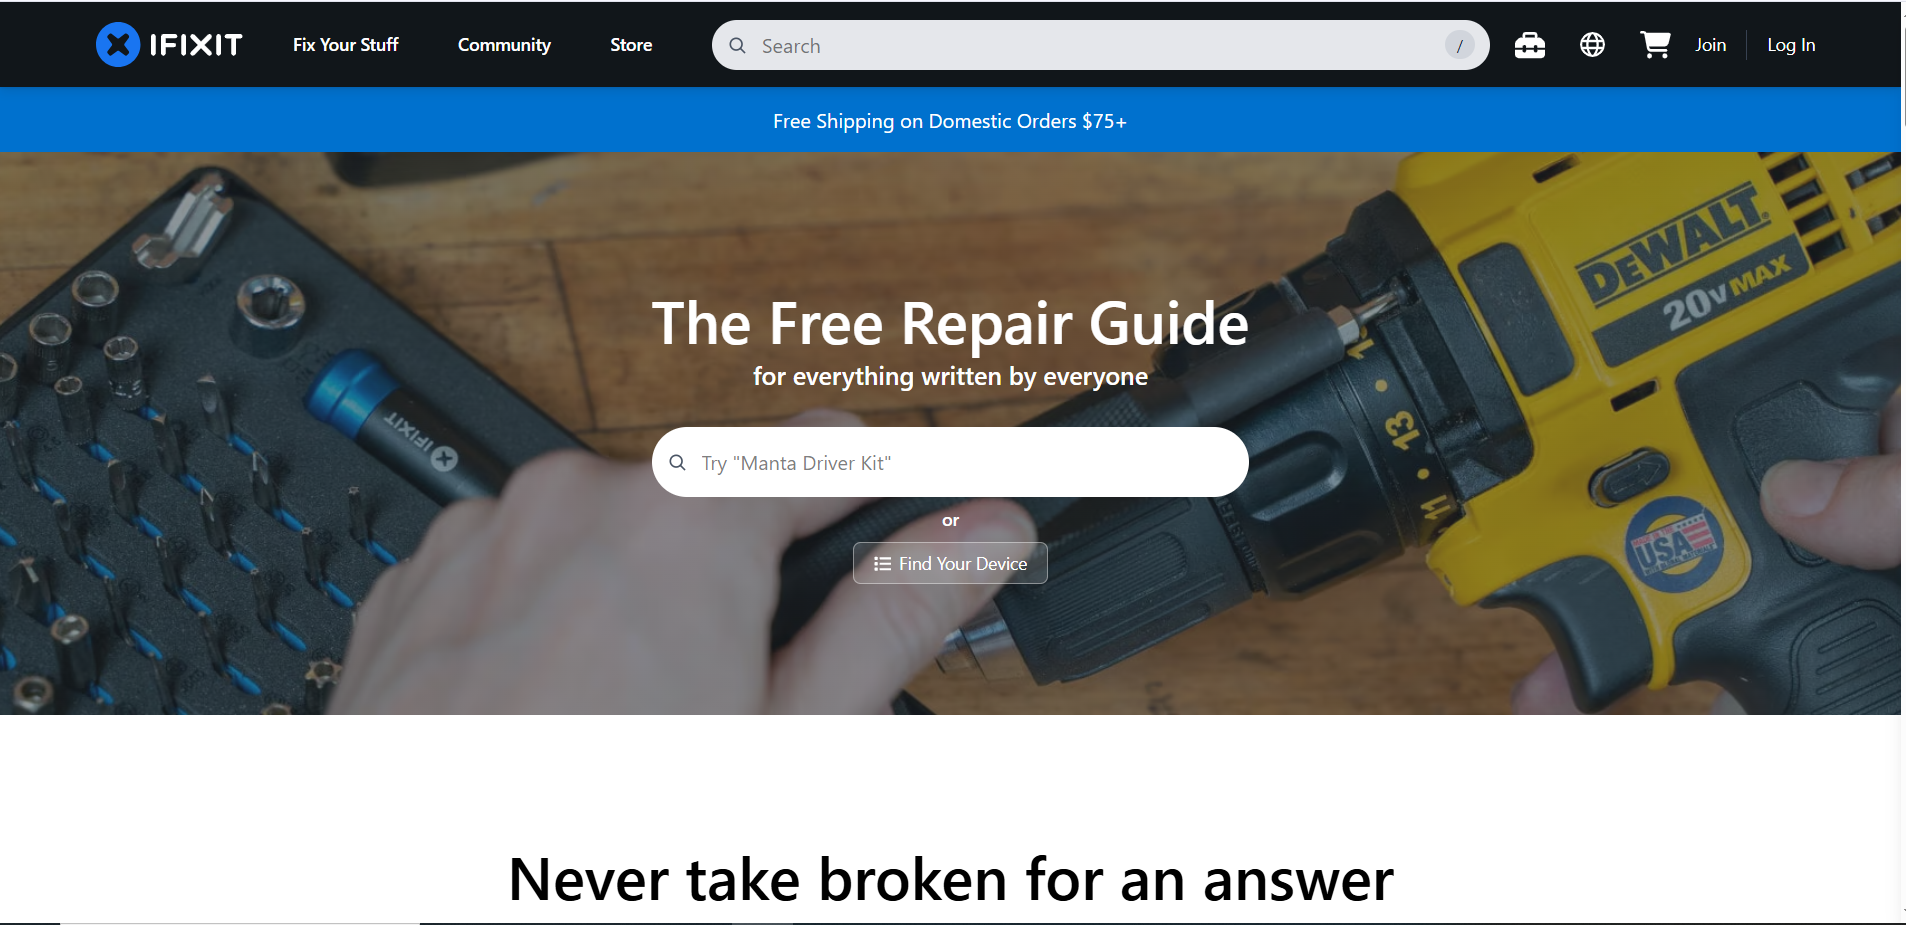
\includegraphics[width=0.7\textwidth]{ifix.PNG}
\caption{iFixit platform interface}
\end{figure}

\paragraph{The GE Appliances Support Portal}
GE Appliances~\cite{geappliances} offers digital manuals and technician bookings through its \textit{SmartHQ} ecosystem. While it includes AI chat tools for home diagnostics, the system is strictly proprietary. Other hardware manufacturers cannot use this ecosystem to support their own products.

\begin{figure}[!htbp]
\centering
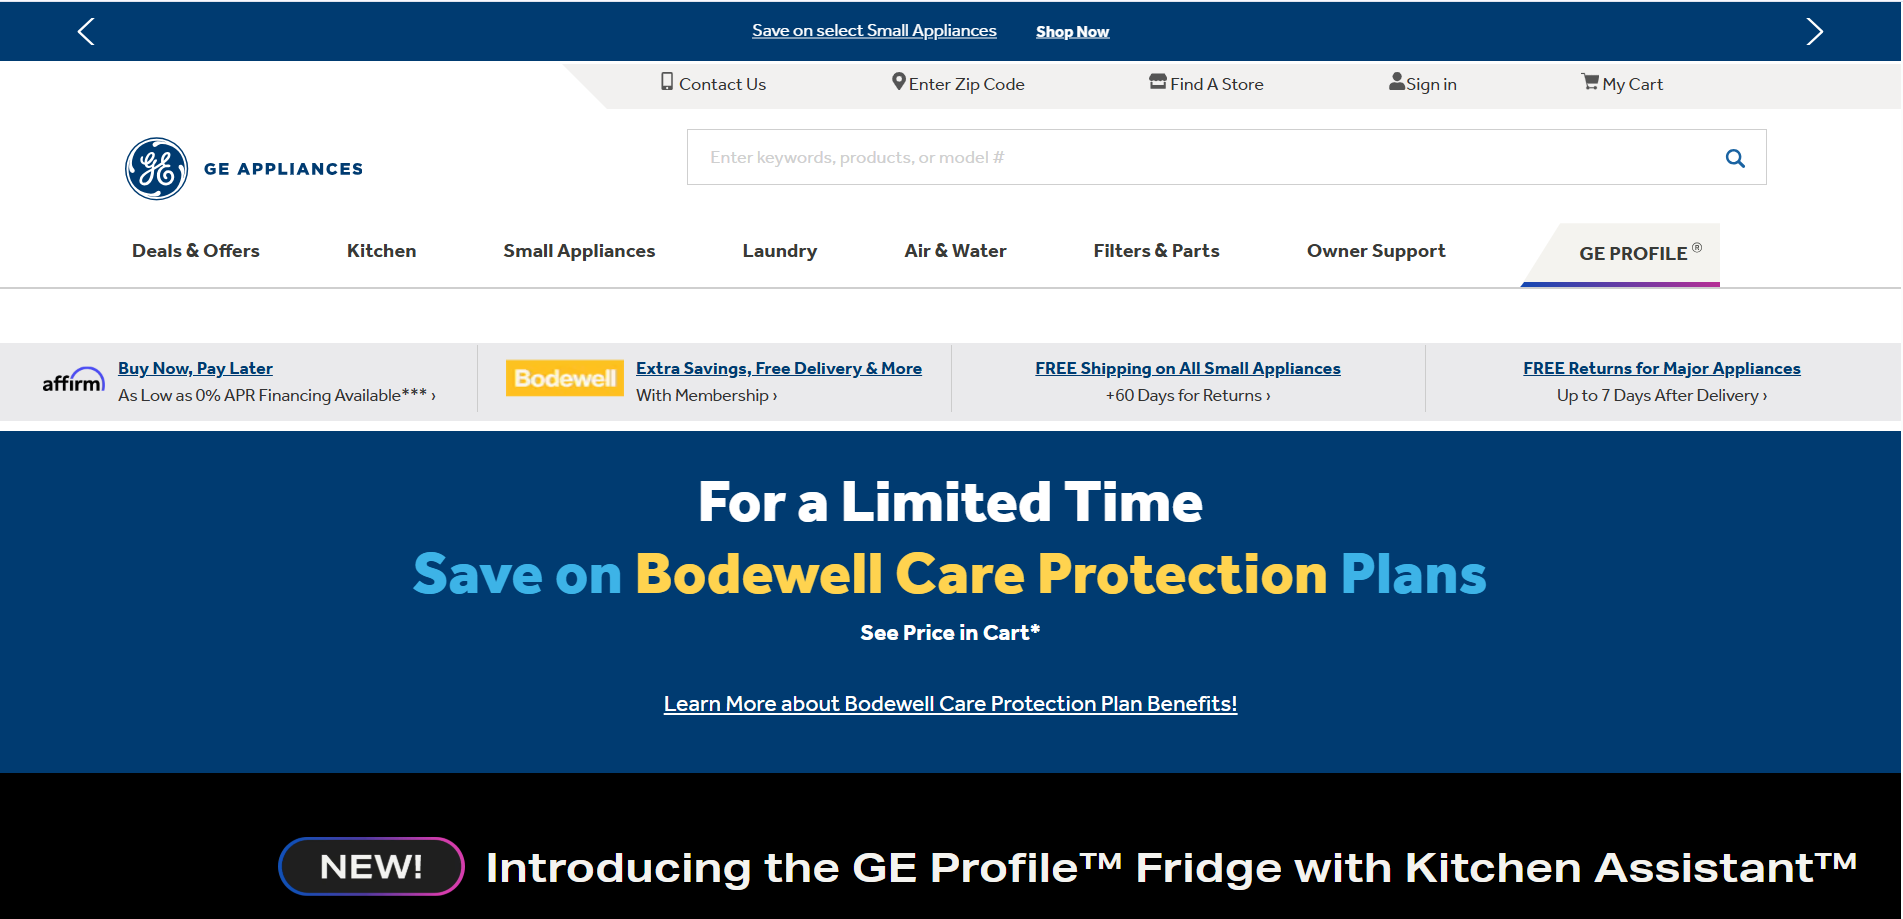
\includegraphics[width=0.7\textwidth]{ge app.PNG}
\caption{GE Appliances support platform}
\end{figure}

\subsubsection{Comparative Study}

To place our project in the market, we compared these existing systems using five core functional metrics.

\begin{table}[!htbp]
\centering
\caption{Comparative study of existing solutions}
\label{tab:comparative_study}
\resizebox{0.85\textwidth}{!}{%
\begin{tabular}{lcc}
\toprule
\textbf{Functional Criterion} & \textbf{iFixit} & \textbf{GE Appliances} \\
\midrule
Primary Access Method & Manual Search & Serial / Model Lookup \\
AI-Assisted Support & Yes (FixBot App) & Yes (SmartHQ App) \\
Content Moderation Model & Wiki / Community & Official / Brand-Specific \\
Multi-Tenant SaaS Architecture & No & No \\
Service Ticketing Integration & No & Brand Repair Scheduling \\
\bottomrule
\end{tabular}%
}
\end{table}

\subsubsection{Comparative Evaluation and Positioning}

Looking at Table~\ref{tab:comparative_study}, we see a clear gap in how product support is handled today. Community-driven platforms like iFixit have plenty of data, but they lack the privacy and brand control that enterprises require. On the other hand, proprietary systems like GE Appliances are highly secure but closed off, meaning other brands cannot use them. 

To bridge this gap, we built \textbf{PRO-WISE} as a multi-tenant, cloud-based SaaS platform. Here is how it stands out:
\begin{itemize}
    \item \textbf{Direct QR Scanning}: Scanning a product QR code drops users straight into a customized troubleshooting space, skipping standard search engines entirely.
    \item \textbf{Smart Moderation}: We combine official developer-written guides with real-time AI screening to keep technical documentation safe and accurate.
    \item \textbf{Built-in Gemini Assistant}: We plugged in a RAG pipeline powered by the Google Gemini API so users can chat with their manuals in natural language.
    \item \textbf{Connected Help Desk}: When self-service troubleshooting fails, users can file a ticket to send the issue directly to a technician.
\end{itemize}

\subsubsection{How PRO-WISE Works End-to-End}

We designed PRO-WISE to link physical machines with smart digital services. Figure~\ref{fig:prowise_workflow} shows how users and administrators interact with the system components.

\begin{figure}[!htbp]
\centering
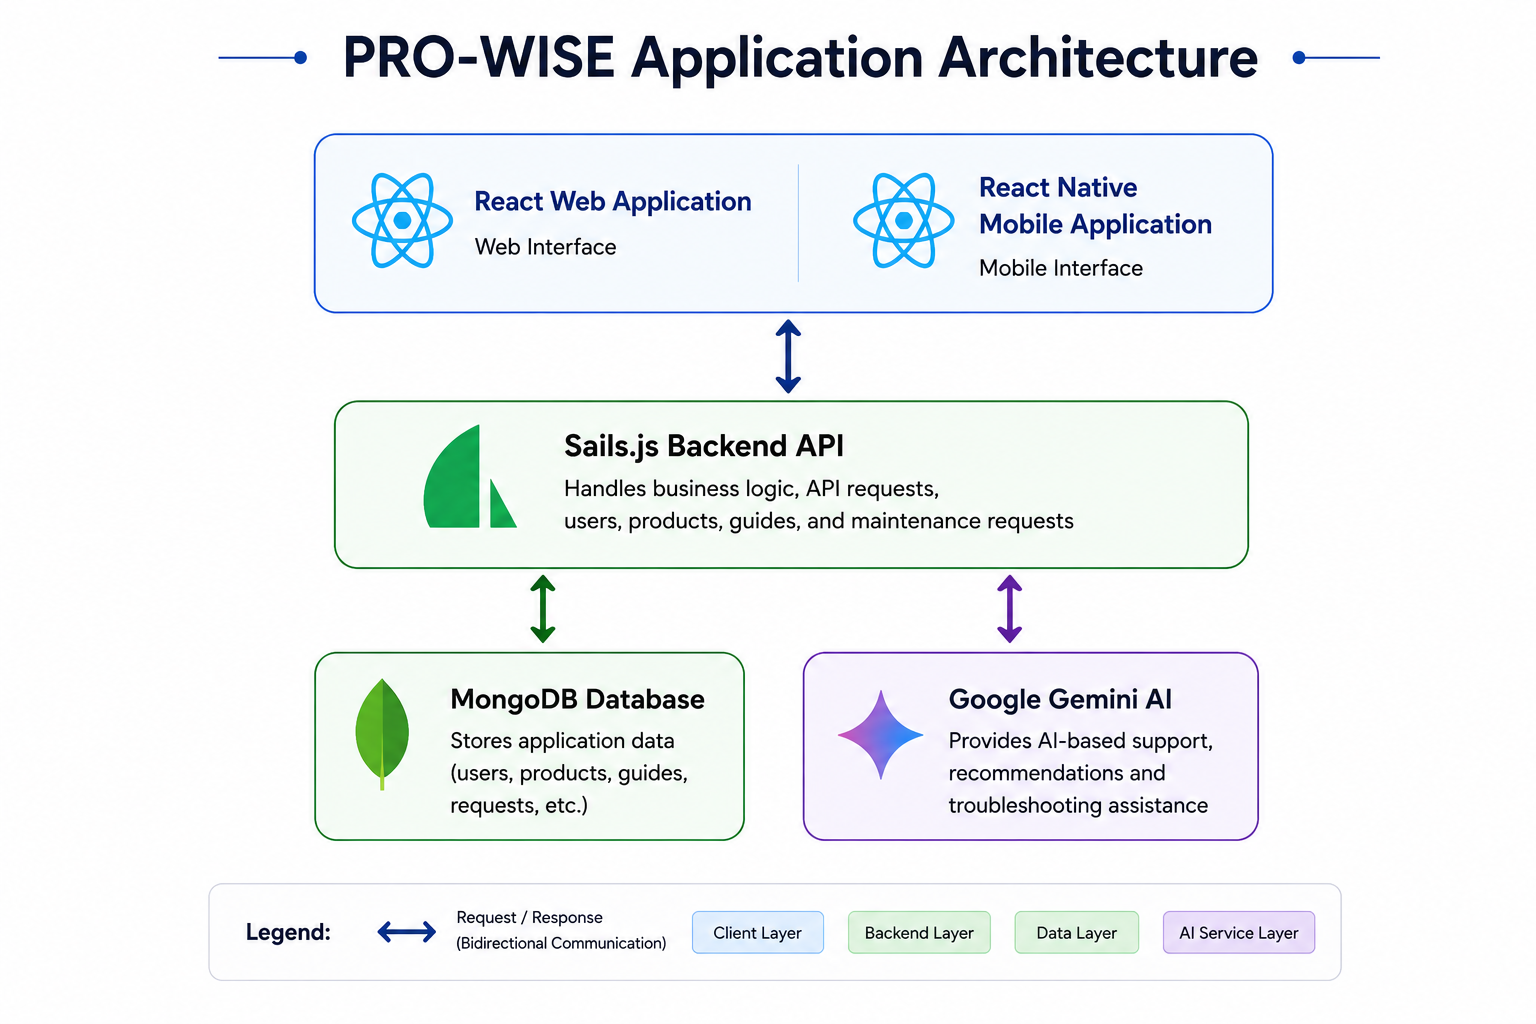
\includegraphics[width=\textwidth,height=0.72\textheight,keepaspectratio]{Archetecture.png}
\caption{PRO-WISE platform operational workflow and high-level architecture}
\label{fig:prowise_workflow}
\end{figure}

Here is the operational workflow step-by-step:
\begin{enumerate}
    \item \textbf{Scanning the QR Code}: A customer scans the product's QR sticker using their phone's camera web or mobile view.
    \item \textbf{Extracting the ID}: The app pulls the unique identifier from the QR code and requests the backend server via HTTPS.
    \item \textbf{Data Fetching}: The backend queries MongoDB for the product's details, PDF steps, and pre-computed text embeddings.
    \item \textbf{Semantic Querying}: If the user asks a question, the backend vectors the text, runs a similarity lookup in MongoDB, and passes the context to Google Gemini to get an exact answer.
    \item \textbf{Rendering the App}: The backend returns the guides, parts listing, and AI replies, showing a clean workspace to the user.
    \item \textbf{Filing a Ticket}: If the problem persists, the user submits a help request, which sends a notification and routes the ticket to available technicians.
\end{enumerate}

\section{Adopted Software Development Methodology}

\subsection{Methodological Rationale}

Building a multi-tenant platform with a mobile client, web dashboard, and custom RAG search is complex. We chose an Agile approach because we needed to adapt quickly to requirement changes. Working f el cycles helped us build and test features piece by piece, getting feedback from our advisors early and often.

\subsection{The Scrum Framework}

To stay organized and deliver real features regularly, we used the Scrum framework~\cite{scrumguide}. We divided our 10-week timeline into five two-week sprints. Since this was a solo project, we had to adapt the roles: my advisors stepped in as Product Owners to help prioritize features, while I wore both the Scrum Master and Developer hats to write code and manage the lifecycle.

\subsection{Project Roles and Mapping}

For this academic graduation project (PFE), we mapped the standard Scrum roles as follows:
\begin{itemize}
    \item \textbf{Product Owner}: Handled jointly by both academic and industry advisors. They were responsible for setting requirements and ranking features in order of importance.
    \item \textbf{Scrum Master}: Managed project timelines and cleared technical obstacles.
    \item \textbf{Development Team}: Handled entirely by the student developer, covering everything from database schemas and API coding to frontend layout design, Gemini integration, and unit testing.
\end{itemize}

\subsection{Scrum Events and Artifacts}

We used standard Scrum practices to organize our sprints:
\begin{itemize}
    \item \textbf{Product Backlog}: The complete, ordered list of features required for the final system.
    \item \textbf{Sprint Backlog}: The specific tasks we committed to finish within the active two-week cycle.
    \item \textbf{Sprints}: Two-week development windows dedicated to building and verifying specific releases.
    \item \textbf{Reviews \& Retrospectives}: Quick evaluations at the end of each sprint to check progress, test features, and plan adjustments for the next cycle.
\end{itemize}

Figure~\ref{fig:scrum_workflow} shows how we adapted the Scrum lifecycle to build PRO-WISE.
        
\begin{figure}[!htbp]
\centering
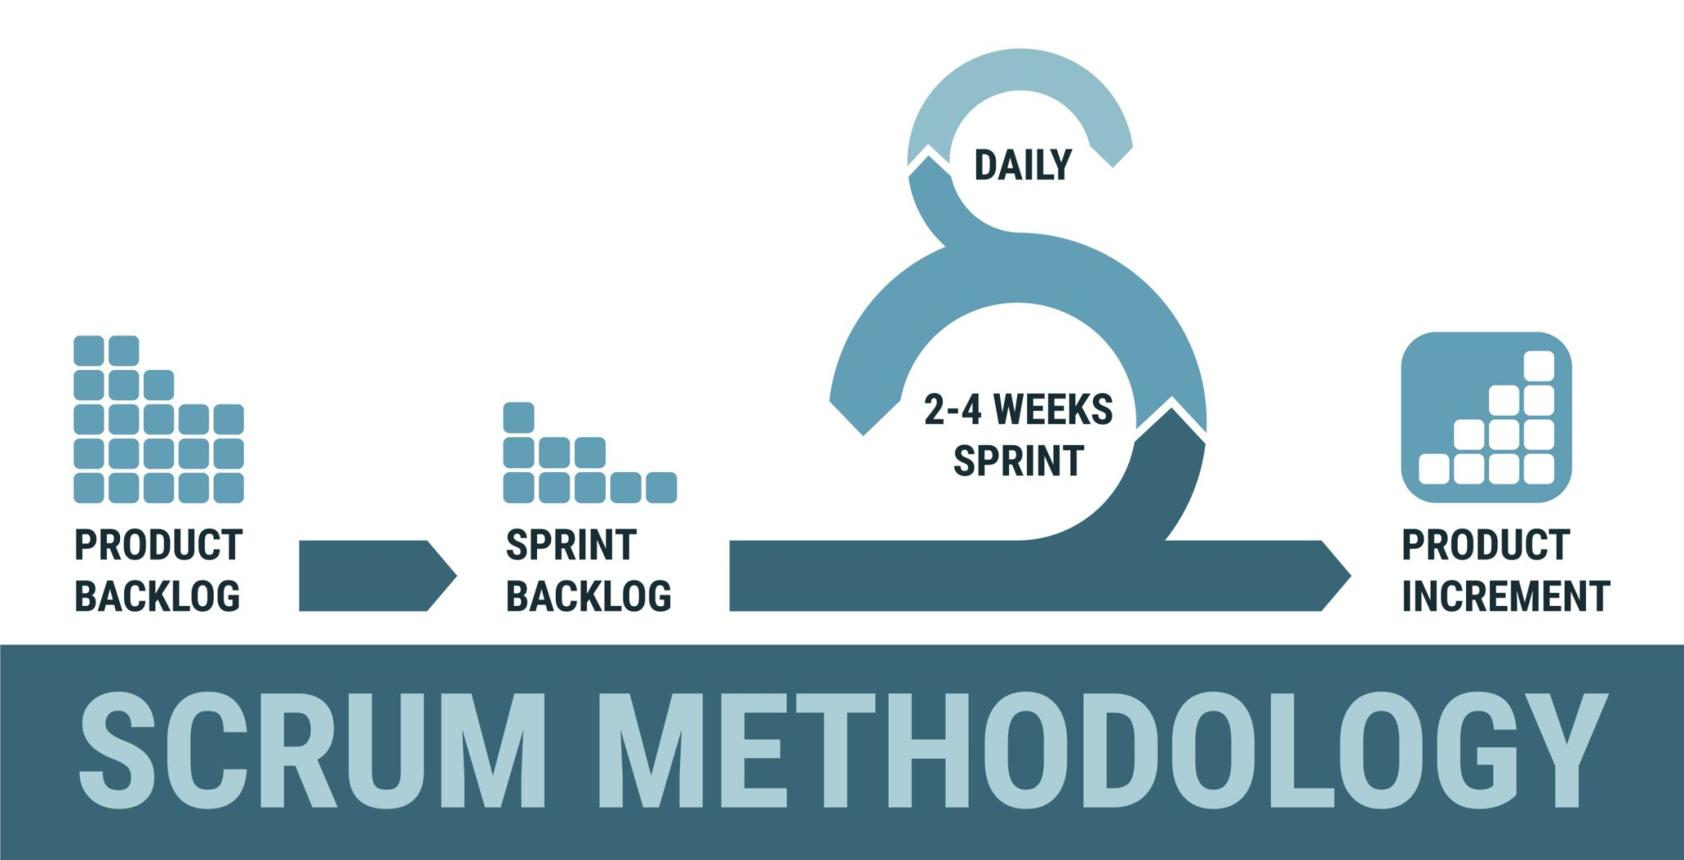
\includegraphics[width=0.92\textwidth]{scrum.jpg}
\caption{Scrum process workflow applied to PRO-WISE development}
\label{fig:scrum_workflow}
\end{figure}

The project schedule and sprint distribution are summarized in Figure~\ref{fig:gantt_planning}.

\begin{figure}[!htbp]
\centering
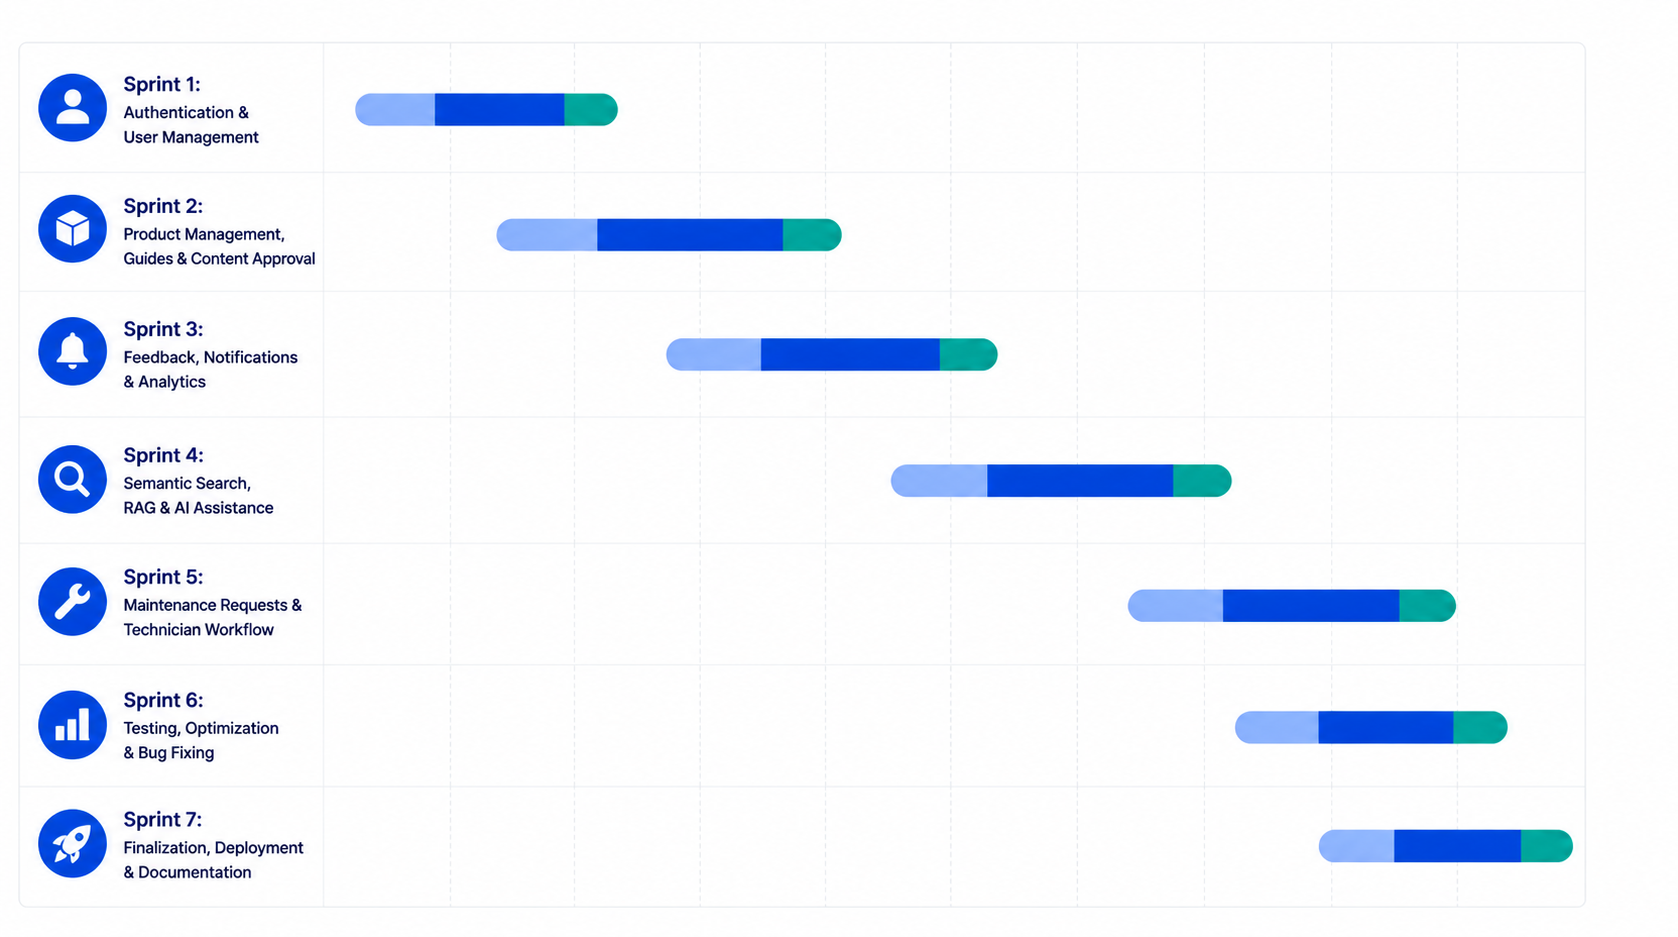
\includegraphics[width=0.85\textwidth]{gant (2).png}
\caption{Gantt chart of the PRO-WISE project planning}
\label{fig:gantt_planning}
\end{figure}

\section{UML Modeling Approach}

We used UML diagrams~\cite{umlguide} to plan out the system before writing code. Designing these models helped us match backlog stories directly to backend Sails.js endpoints and database structures. We focused on three main types of diagrams:
\begin{itemize}
    \item \textbf{Use Case Diagrams}: These show who is using the app and what actions they are allowed to perform.
    \item \textbf{Class Diagrams}: These model our MongoDB database schemas and the relationships between collections.
    \item \textbf{Sequence Diagrams}: These trace the exact order of API requests, middleware checks, and database updates between the UI and Sails.js.
\end{itemize}
The detailed specifications and specific designs for each diagram type are integrated within the corresponding requirements and sprint release chapters.

\section{Conclusion}

We started by presenting our host company, Accelerant, and examining the real-world repair challenges that PRO-WISE addresses. We compared our system against market competitors like iFixit and GE Appliances to show where we stand. Lastly, we introduced the Agile Scrum workflow and UML models we used to map the application logic. The next chapter goes into system architecture, requirements capture, and the product backlog.

\chapter{Architecture, Tools and Development Environment}

\section{Introduction}

In this chapter, we go under the hood of the PRO-WISE platform. We list the actors who interact with the system, outline the core functions, and describe the performance and security standards. We also detail the product backlog, system architecture diagram, tech stack, and development environment setup.

\section{Requirements Capture}

\subsection{Actors Identification}

We defined five main actors who interact with the system:

\begin{itemize}
    \item \textbf{Client}: Scans QR codes, views repair guides, watches troubleshooting videos, asks questions to the AI assistant, and leaves ratings.
    \item \textbf{Technician}: Edits guides, uploads photos or videos from site visits, handles ticket requests, and uses Gemini to draft manuals.
    \item \textbf{Company Admin}: Manages the brand's catalog (products, models), adds team members, and approves guide drafts before publication.
    \item \textbf{Super Admin}: Registers new manufacturing brands, updates system-wide configs, and inspects security audit logs.
    \item \textbf{AI System}: An automated background actor that computes text embeddings, ranks compatibility recommendations, and checks content quality.
\end{itemize}

\subsection{Functional Requirements}

We grouped the functional features into key modules. We designed each module to support multi-tenant isolation, ensuring brands cannot access each other's data~\cite{mongodb_multitenant}:

\begin{itemize}
    \item \textbf{Authentication}: Role-based permissions (Client, Technician, Company Admin, Super Admin) managed via JWT and Google login, enforcing brand isolation.
    \item \textbf{Catalog Management}: Administrative panels for company managers to handle products, manuals, and category links.
    \item \textbf{Guides Editor}: An interface for technicians to write step-by-step repair guides instead of just uploading static documents.
    \item \textbf{Intelligent Search}: Leveraging the Gemini API \cite{gemini} for semantic document queries, product recommendations, and language translation.
    \item \textbf{Maintenance Ticketing}: A portal for users to submit help requests and company managers to dispatch technicians.
    \item \textbf{QR Routing}: Generating barcodes linked to specific models that redirect users directly to help pages.
\end{itemize}

\subsection{Non-Functional Requirements}

To ensure the app is fast, secure, and reliable under heavy load, we met the following performance benchmarks:

\begin{itemize}
    \item \textbf{Security}: Security was our top priority. We hashed all passwords using bcrypt with 10 salt rounds to block brute force attempts. For network security, we set up TLS 1.3 across all endpoints. We also protected the API against XSS and CSRF by storing stateless HS256-signed JWTs directly in HTTP-only, Secure, and SameSite=Strict cookies. It's clean and safe.
    \item \textbf{Performance}: We wanted the app to feel fast, aiming for sub-2-second loads. We audited pages with Lighthouse~\cite{lighthouse} to optimize assets, hosting images on a CDN. In MongoDB, we avoided heavy offsets by using cursor-based pagination and created compound indexes on query-heavy fields to keep response times low.
    \item \textbf{Responsive UI}: We styled the frontend with Flexbox and CSS Grid so it adapts to any screen, keeping WCAG 2.1 AA guidelines in mind. On mobile, the React Native app uses viewport scaling, making sure buttons and text look good on any screen size from 4 to 6.7 inches.
    \item \textbf{Uptime}: To handle traffic spikes, we used Nginx~\cite{nginx} as a reverse proxy and load balancer. We also set up MongoDB as a three-node replica set. If one database node goes down, the system handles the failover automatically without interrupting the user.
    \item \textbf{Code Quality}: We separated business logic into Sails.js services to keep controllers thin and clean. Code format is enforced using ESLint~\cite{eslint}. On the client, we went with Redux Toolkit for state management, keeping everything type-safe with strict TypeScript.
\end{itemize}

\subsection{Product Backlog}

\renewcommand{\arraystretch}{1.3}
\setlength{\tabcolsep}{8pt}

\begin{longtable}{clp{8cm}c}
\caption{Product Backlog of PRO-WISE Platform} \label{tab:product_backlog} \\
\toprule
\textbf{ID} & \textbf{Feature / Epic} & \textbf{Description} & \textbf{Priority} \\
\midrule
\endfirsthead

\toprule
\textbf{ID} & \textbf{Feature / Epic} & \textbf{Description} & \textbf{Priority} \\
\midrule
\endhead

\midrule
\multicolumn{4}{r}{\textit{Continued on next page}} \\
\bottomrule
\endfoot

\bottomrule
\endlastfoot

1 & Authentication System & User login and registration using JWT and Google OAuth 2.0 & High \\
2 & Role Management & Role-based access control for different user types & High \\
3 & User Approval & Validation of administrator and technician accounts & High \\
4 & Category Management & Management of predefined product categories & High \\
5 & Company Management & Company creation and profile management & High \\
6 & Product Management & CRUD operations for products linked to companies & High \\
7 & QR Code System & Generation and scanning of QR codes for product access & High \\
8 & Product Details Page & Display of product information, guides, and media & High \\
9 & Guide Management & Creation of structured guides with step-by-step instructions & High \\
10 & Media Support & Upload and management of PDFs, videos, and images & High \\
11 & Content Approval System & Validation workflow for content publication & High \\
12 & Feedback System & User ratings and comments & Medium \\
13 & Recommendation System & Similarity-based product and component recommendations using product metadata and embeddings & Medium \\
14 & Similar Products & Display of related products within product pages & Medium \\
15 & Search System & Semantic search for products and content using Gemini embeddings and cosine similarity ranking & Medium \\
16 & Technician Module & Upgrade users to technicians with service profiles & High \\
17 & Maintenance Services & Creation and follow-up of repair requests between users and technicians & Medium \\
18 & Analytics System & Tracking of system usage and activity & Medium \\
19 & Activity Logs & Recording system actions for monitoring & Medium \\
20 & Notification System & User notifications for updates and actions & Medium \\
21 & UI/UX Redesign & Improvement of web and mobile interfaces & Medium \\
22 & Mobile Application & Development of mobile experience & High \\
23 & Web Admin Dashboard & Administrative interfaces for system management & High \\
24 & Performance Optimization & Optimization of system performance & Medium \\
25 & Testing and Bug Fixing & Ensuring system stability and reliability & High \\
26 & Security Enhancements & Implementation of secure APIs and validation & High \\
27 & Documentation (PFE) & Final report and technical documentation & High \\
\end{longtable}

\textbf{Priority Level Legend:}
\begin{itemize}
    \item High: Critical priority, addressing core functionalities and system security.
    \item Medium: Moderate priority, covering auxiliary features, optimization, and enhancements.
\end{itemize}

\section{Diagrams}

\subsection{Global Use Case Diagram}

The global use case diagram in Figure~\ref{fig:global_usecase} maps out how each actor interacts with our system's services. We define four main roles:
\begin{itemize}
    \item \textbf{Customer:} Browses products, writes ratings, and submits ticketing requests.
    \item \textbf{Technician:} Resolves customer support tickets, edits troubleshooting guides, and uses Gemini drafts to write manuals.
    \item \textbf{Company Admin:} Manages the brand catalog, registers employees, and manually checks submitted guides.
    \item \textbf{AI-System:} An automated background worker (powered by Gemini) that runs semantic searches, auto-approves quality drafts, and translates texts without manual admin oversight.
\end{itemize}

\begin{figure}[!htbp]
\centering
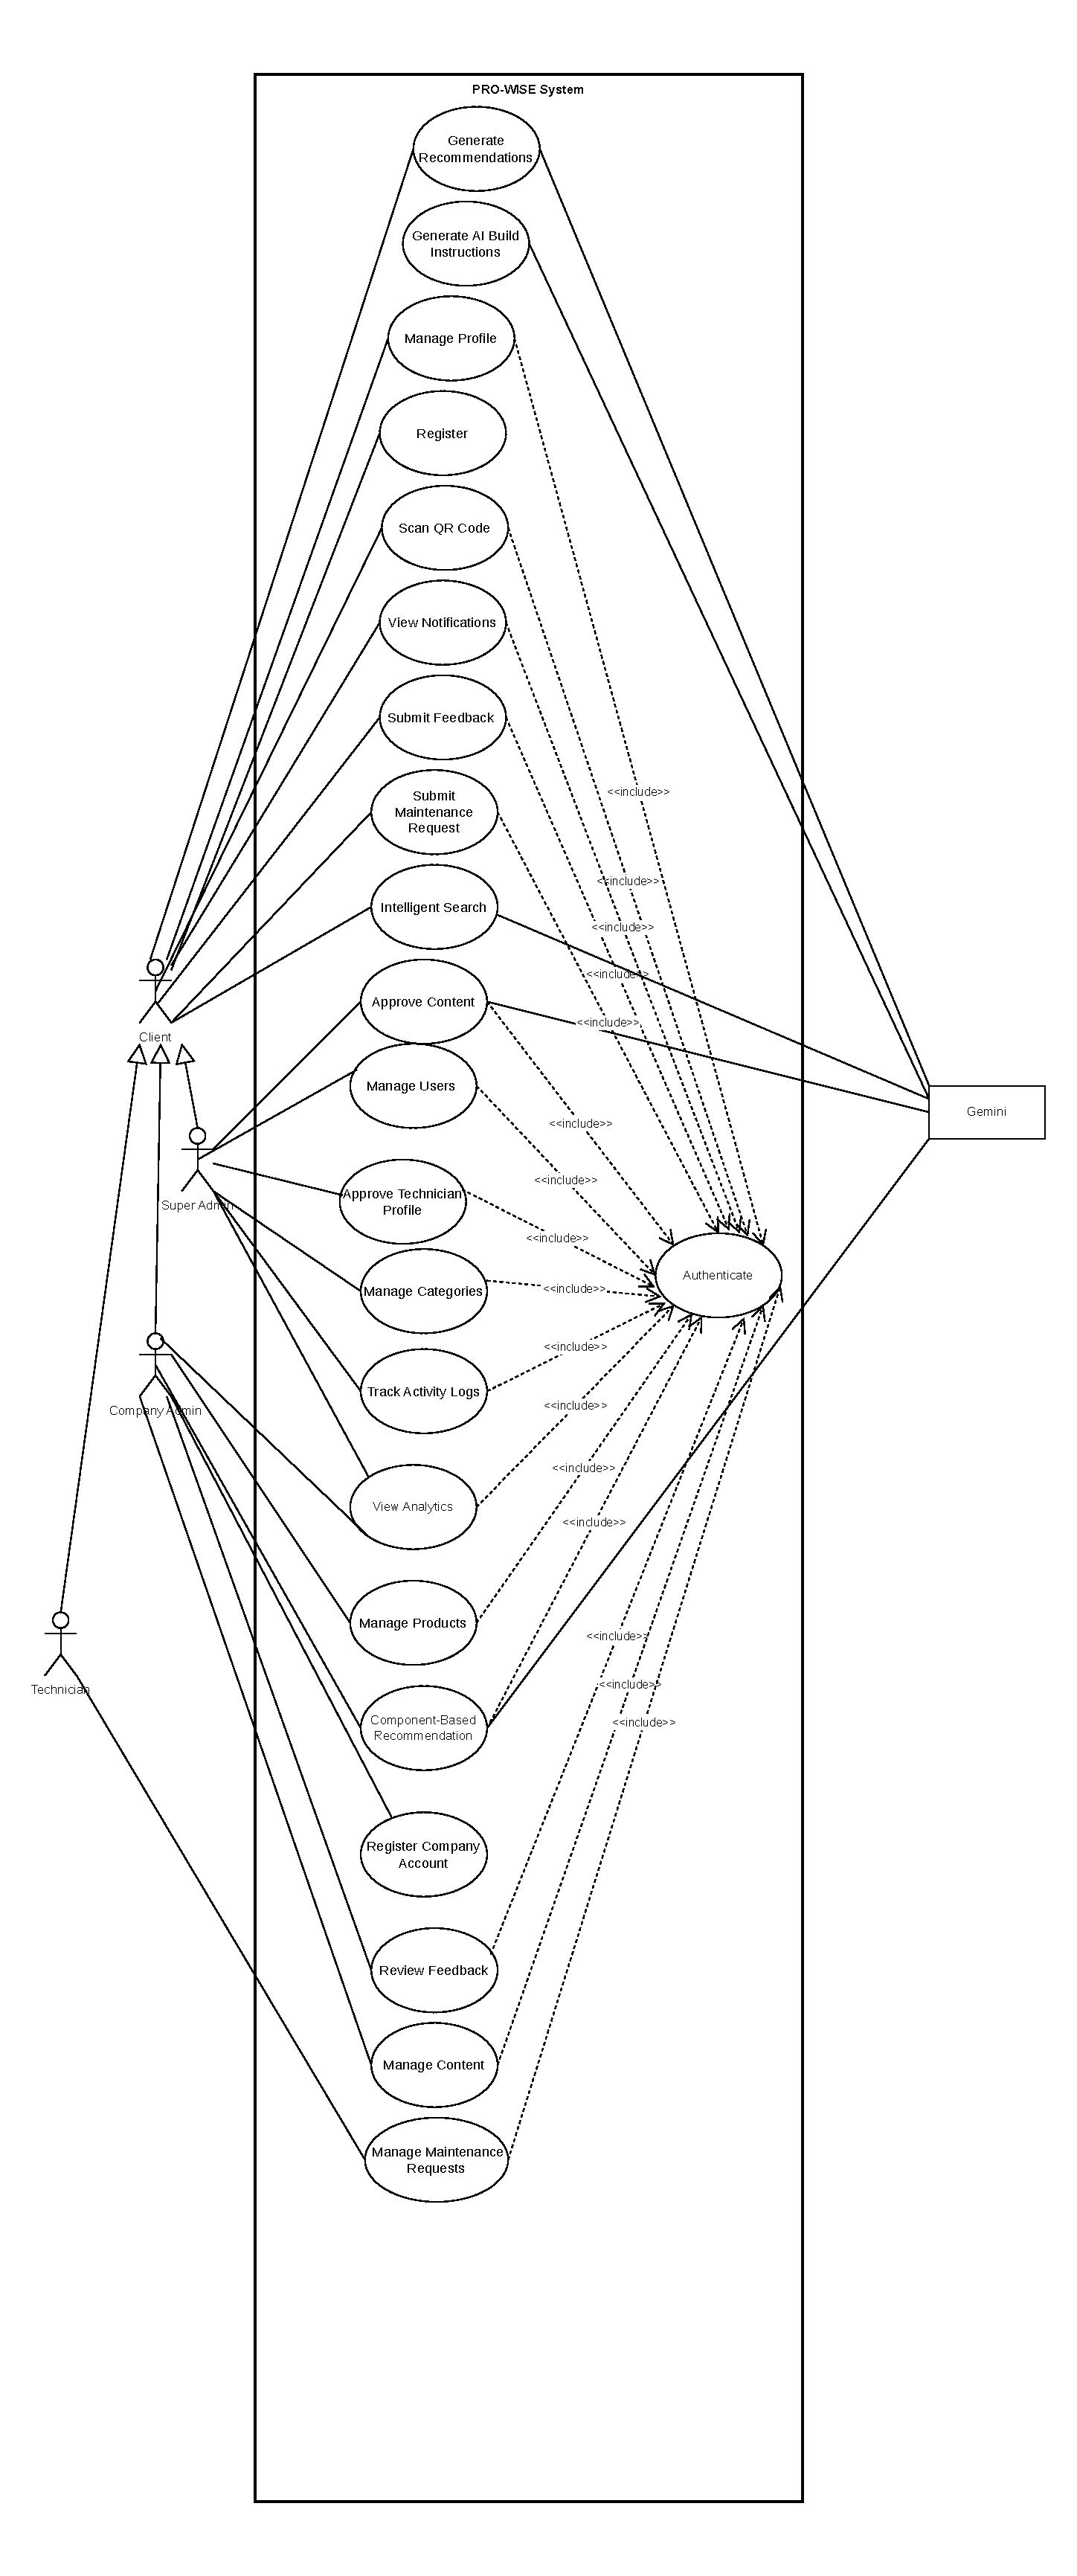
\includegraphics[width=\textwidth,height=0.82\textheight,keepaspectratio]{images/global_usecase.pdf}
\caption{Global use case diagram of PRO-WISE}
\label{fig:global_usecase}
\end{figure}

\subsection{Global Class Diagram}

The global class diagram in Figure~\ref{fig:global_class_diagram} shows the database schema for the PRO-WISE system. It highlights our MongoDB models (auth, catalog management, feedback, and maintenance tickets), detailing fields, data types, and relationships.

\begin{figure}[!htbp]
\centering
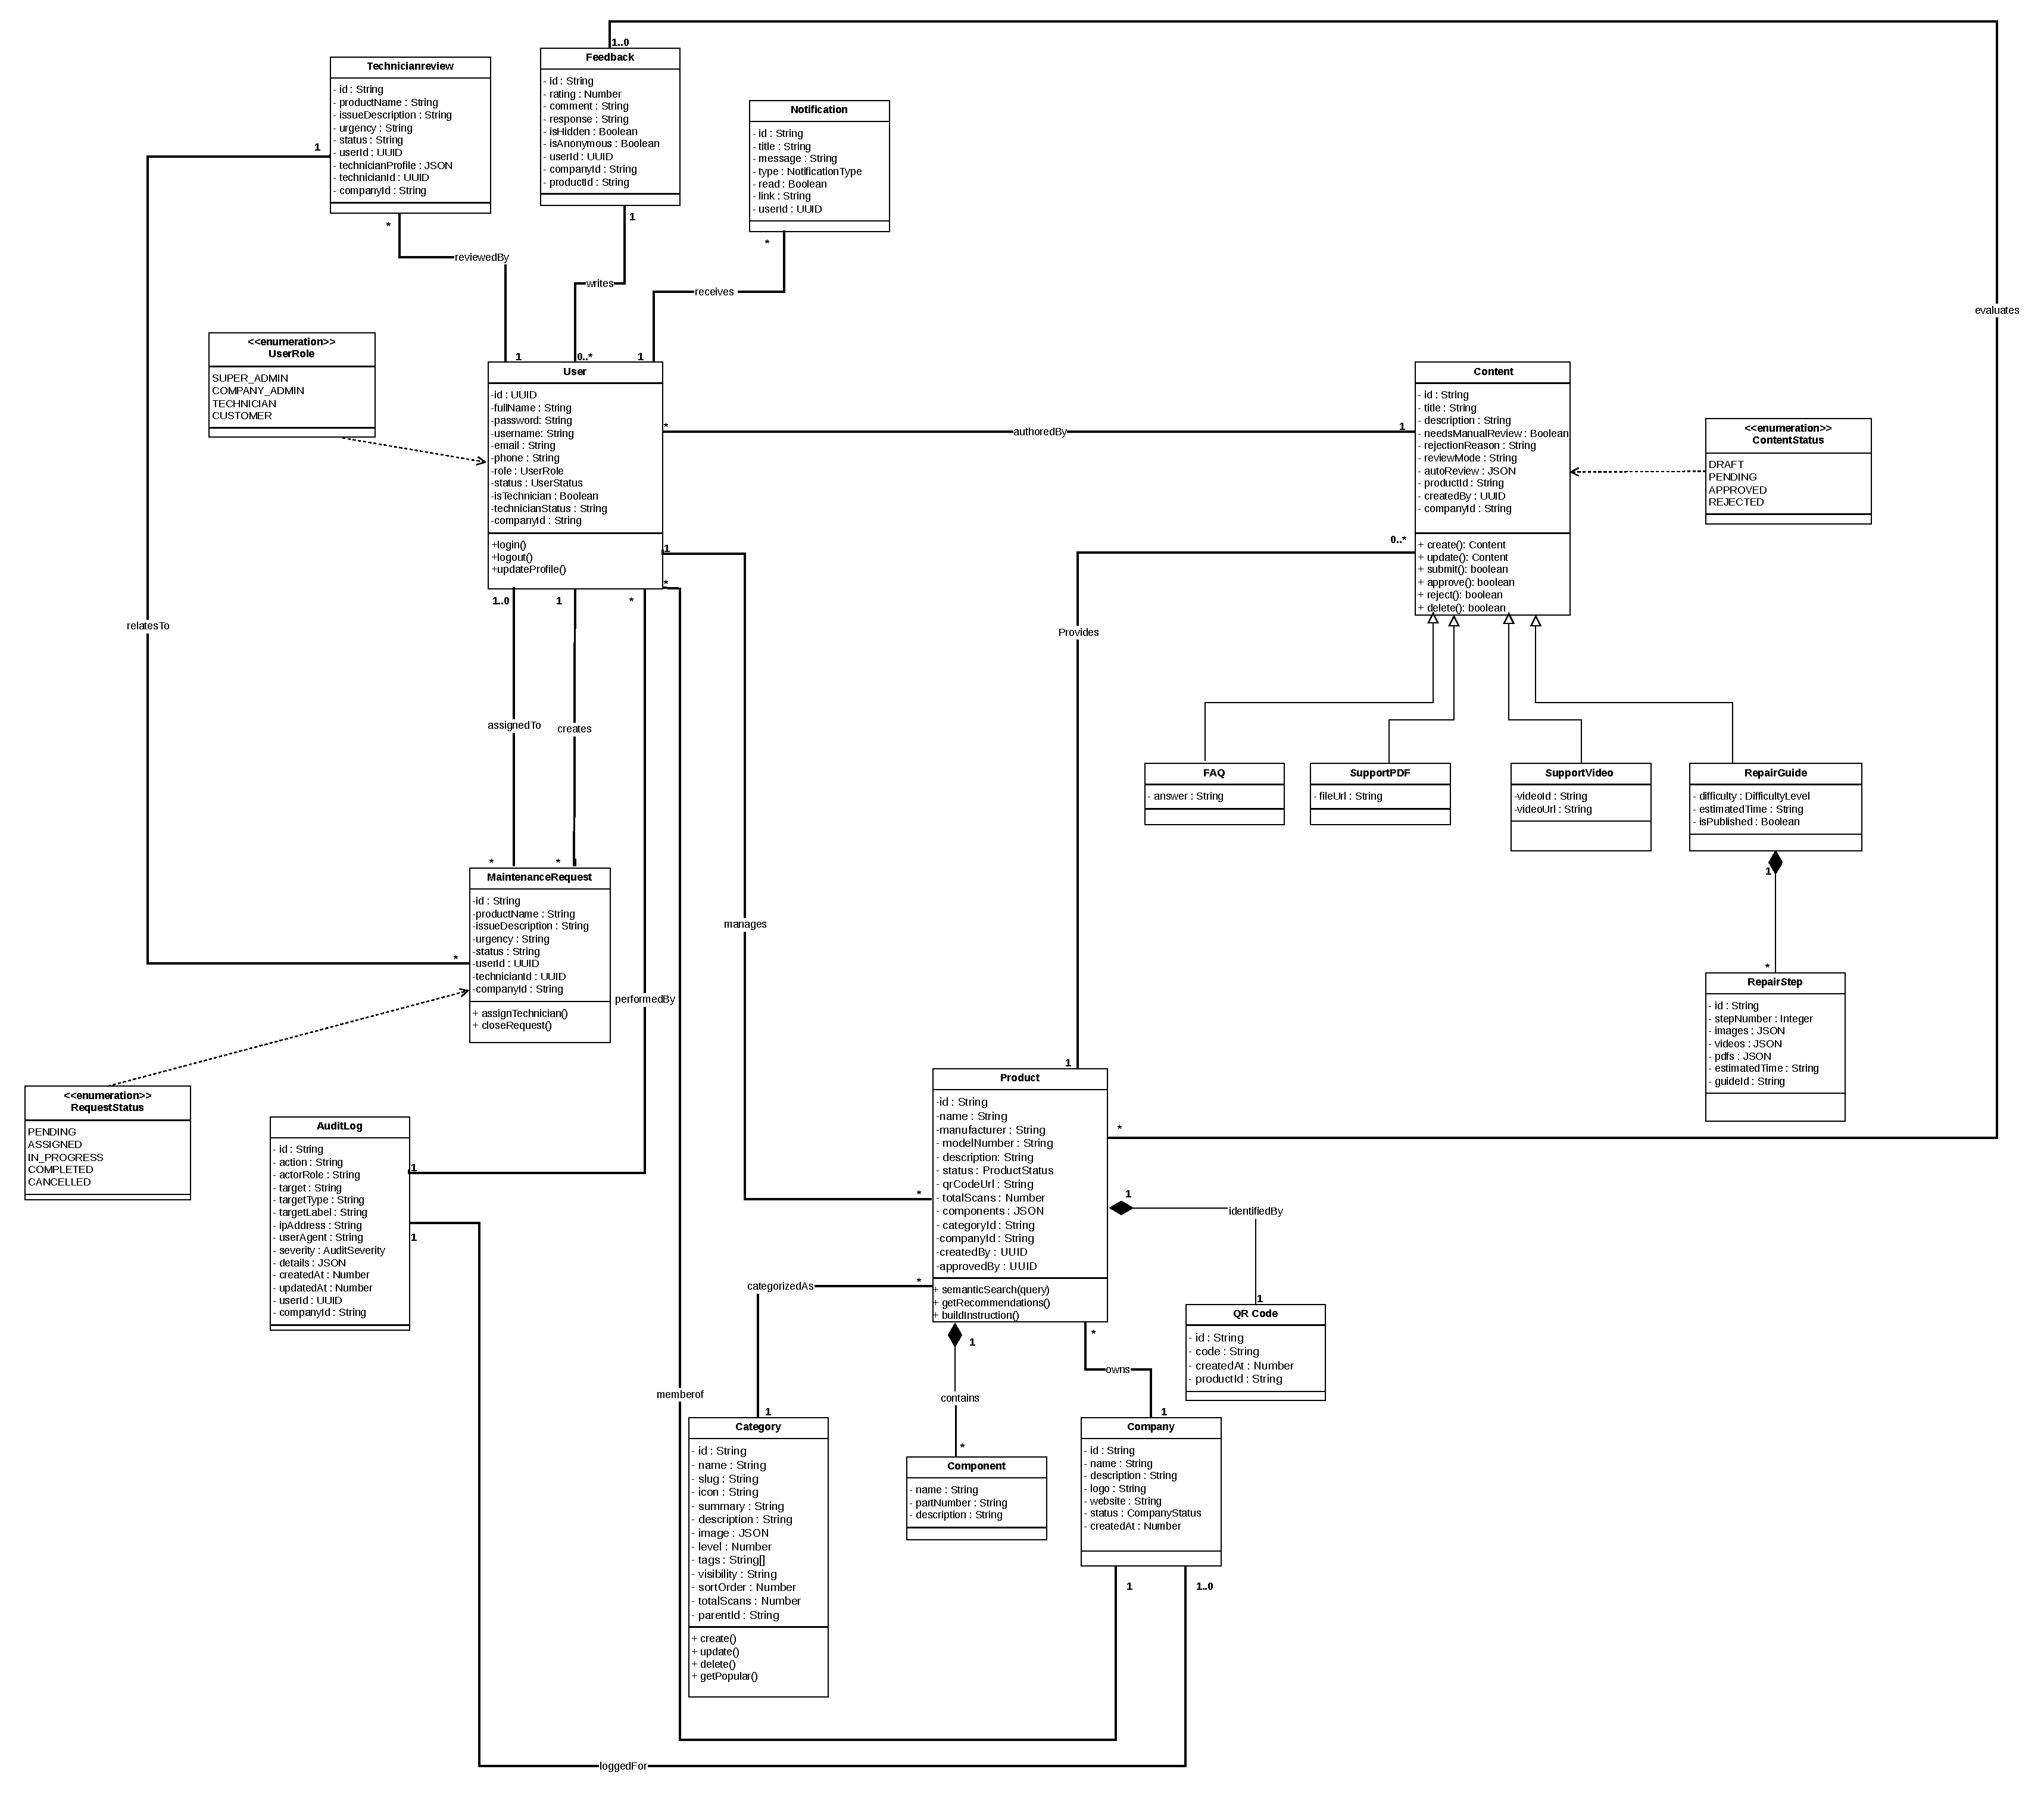
\includegraphics[width=\textwidth,height=0.82\textheight,keepaspectratio]{images/global_class_diagram.pdf}
\caption{Global class diagram of the system}
\label{fig:global_class_diagram}
\end{figure}

\subsection{Application Architecture}

We built the codebase inside a monorepo containing three applications. The backend REST API runs on Node.js~\cite{nodejs} and Sails.js~\cite{sailsjs}, communicating with MongoDB~\cite{mongodb} using the \texttt{sails-mongo} driver. The web dashboard is built with React~\cite{react}, Vite~\cite{vite}, and TypeScript~\cite{typescript}, using Redux Toolkit~\cite{redux} to manage app state. The mobile client utilizes React Native~\cite{reactnative} and Expo~\cite{expo}, handles QR code scanning using the camera API~\cite{qrcode}, and navigates screens via React Navigation.

\begin{figure}[!htbp]
\centering
\resizebox{\textwidth}{!}{%
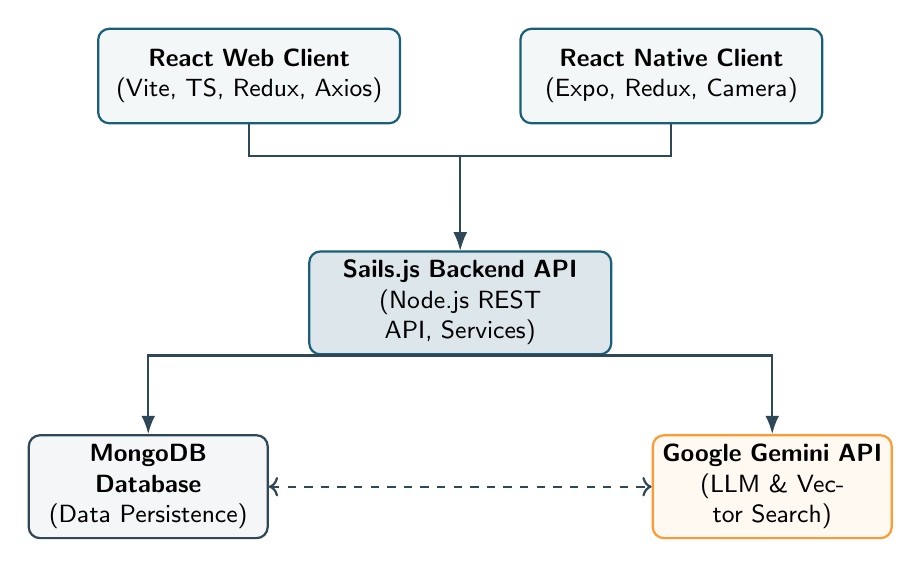
\begin{tikzpicture}[
    node distance=1.2cm and 1.5cm,
    block/.style={rectangle, draw=industrialblue, fill=industrialblue!5, thick, rounded corners, minimum width=3.8cm, minimum height=1.2cm, align=center, text width=3.6cm, font=\small},
    db/.style={rectangle, draw=slategray, fill=slategray!5, thick, rounded corners, minimum width=3.0cm, minimum height=1.2cm, align=center, text width=2.8cm, font=\small},
    api/.style={rectangle, draw=orange!80, fill=orange!5, thick, rounded corners, minimum width=3.0cm, minimum height=1.2cm, align=center, text width=2.8cm, font=\small},
    arrow/.style={-Latex, thick, slategray}
]
    % Frontend Layer
    \node[block] (web) {\textbf{React Web Client} \\ (Vite, TS, Redux, Axios)};
    \node[block, right=1.5cm of web] (mobile) {\textbf{React Native Client} \\ (Expo, Redux, Camera)};
    
    % Midpoint helper
    \node[coordinate, below=0.6cm of $(web.south)!0.5!(mobile.south)$] (midpoint) {};
    
    % Backend Layer
    \node[block, below=1.0cm of midpoint, draw=industrialblue, fill=industrialblue!15] (backend) {\textbf{Sails.js Backend API} \\ (Node.js REST API, Services)};
    
    % Data & AI Layer
    \node[db, below left=1.0cm and 0.5cm of backend] (db) {\textbf{MongoDB Database} \\ (Data Persistence)};
    \node[api, below right=1.0cm and 0.5cm of backend] (ai) {\textbf{Google Gemini API} \\ (LLM \& Vector Search)};
    
    % Connections
    \draw[arrow] (web.south) -- ++(0,-0.4) -| (backend.north);
    \draw[arrow] (mobile.south) -- ++(0,-0.4) -| (backend.north);
    \draw[arrow] (backend.south) -| (db.north);
    \draw[arrow] (backend.south) -| (ai.north);
    
    % Bidirectional arrow between DB and AI
    \draw[arrow, <->, dashed] (db.east) -- (ai.west);
\end{tikzpicture}%
}
\caption{Application architecture of the PRO-WISE platform}
\end{figure}

\section{Tools and Development Environment}

\subsection{Hardware Environment}

The development was carried out using a personal computer with the following specifications:

\begin{itemize}
    \item Processor: Intel Core i5-6300U CPU @ 2.40GHz
    \item RAM: 16 GB DDR3
    \item Storage: 512 GB SSD
    \item OS: Windows 10 Pro 64-bit
\end{itemize}

\subsection{Technical Environment}

We selected a modern software stack to keep the platform fast, secure, and easy to maintain.

\begin{table}[H]
\centering
\caption{Technologies and tools used in the PRO-WISE platform}
\renewcommand{\arraystretch}{1.4}
\setlength{\tabcolsep}{8pt}
\begin{tabular}{>{\centering\arraybackslash}m{2.2cm}p{4.2cm}p{7.2cm}}
\toprule
\textbf{Logo} & \textbf{Technology / Tool} & \textbf{Role in the project} \\
\midrule
\techlogo{react.png} & React & Development of the dynamic web client interface. \\
\techlogo{expo (1).png} & React Native / Expo & Development and testing of the cross-platform mobile application. \\
\techlogo{sails.png} & Sails.js & Backend REST API, controllers, services, and business logic. \\
\techlogo{Mongodb.png} & MongoDB & NoSQL database used for persistent and flexible data storage. \\
\techlogo{gemini.png} & Google Gemini API \cite{gemini} & AI services for semantic search, recommendations, and generated assistance. \\
\techlogo{Git.png} & Git~\cite{git} & Version control and source code history management. \\
\techlogo{vs.png} & Visual Studio Code~\cite{vscode} & Main source code editor used during implementation. \\
\techlogo{overleaf.png} & Overleaf~\cite{overleaf} & LaTeX writing, formatting, and report preparation support. \\
\techlogo{draw.png} & Draw.io~\cite{drawio} & Creation of UML diagrams and technical architecture illustrations. \\
\bottomrule
\end{tabular}
\end{table}

\section{Conclusion}

In this chapter, we reviewed the project's technical specifications, structural design, UML models, and local setup. With these blueprints ready, we started building the core features. In the next chapter, we walk through Release 1, detailing the authentication system, password hashing, and user roles.

\chapter{Release 1 : Authentication and User Management}

\section{Introduction}

We began development by implementing the platform's core security and account management. This chapter details our implementation of Release 1. Our main objective was setting up a secure, role-isolated tenant boundary so different accounts can access only their specific brand catalogs.

Our implementation focused on three primary areas:
\begin{itemize}
    \item \textbf{Token-based Logins}: We built a stateless authentication system using JSON Web Tokens (JWT~\cite{jwt}) and integrated Google OAuth 2.0~\cite{oauth2}.
    \item \textbf{Role-Based Permissions}: We defined concrete privileges for Clients, Technicians, Company Admins, and Super Admins.
    \item \textbf{Profile Forms}: We created custom profile views to collect basic user info and technical credentials.
\end{itemize}

\section{Sprint Backlog -- Authentication and User Management}

We prioritized five user stories for the initial two-week sprint backlog, focusing on access control and basic security setup. Table~\ref{tab:sprint1_backlog} lists their priority levels and scope.

\renewcommand{\arraystretch}{1.3}
\setlength{\tabcolsep}{8pt}

\begin{table}[!htbp]
\centering
\caption{User stories for Release 1 (Authentication and User Management)}
\label{tab:sprint1_backlog}
\resizebox{\textwidth}{!}{%
\begin{tabular}{clp{8cm}c}
\toprule
\textbf{ID} & \textbf{Feature / Epic} & \textbf{Description} & \textbf{Priority} \\
\midrule
1 & Authentication System & User login and registration using JWT and Google OAuth 2.0 & High \\
2 & Role Management & Role-based access control for different user types & High \\
3 & User Approval & Validation of administrator and technician accounts & High \\
26 & Security Enhancements & Implementation of secure APIs and validation mechanisms & High \\
25 & Testing and Bug Fixing & Ensuring system stability and reliability & High \\
\bottomrule
\end{tabular}%
}
\end{table}

\section{Refinement of Use Cases}

To map out API endpoints and UI routing, we refined three core use cases. We drafted UML diagrams and defined preconditions, postconditions, and nominal flows.

\subsection{Refinement of Sprint 1 Use Cases}

\subsubsection{Use Case Refinement: Register}

When a visitor registers, they must select a role. Figure~\ref{fig:usecase_register} and Table~\ref{tab:register_desc} show how we handle registration. Clients gain access immediately, but technicians and administrators require manual approval.

\begin{figure}[!htbp]
\centering
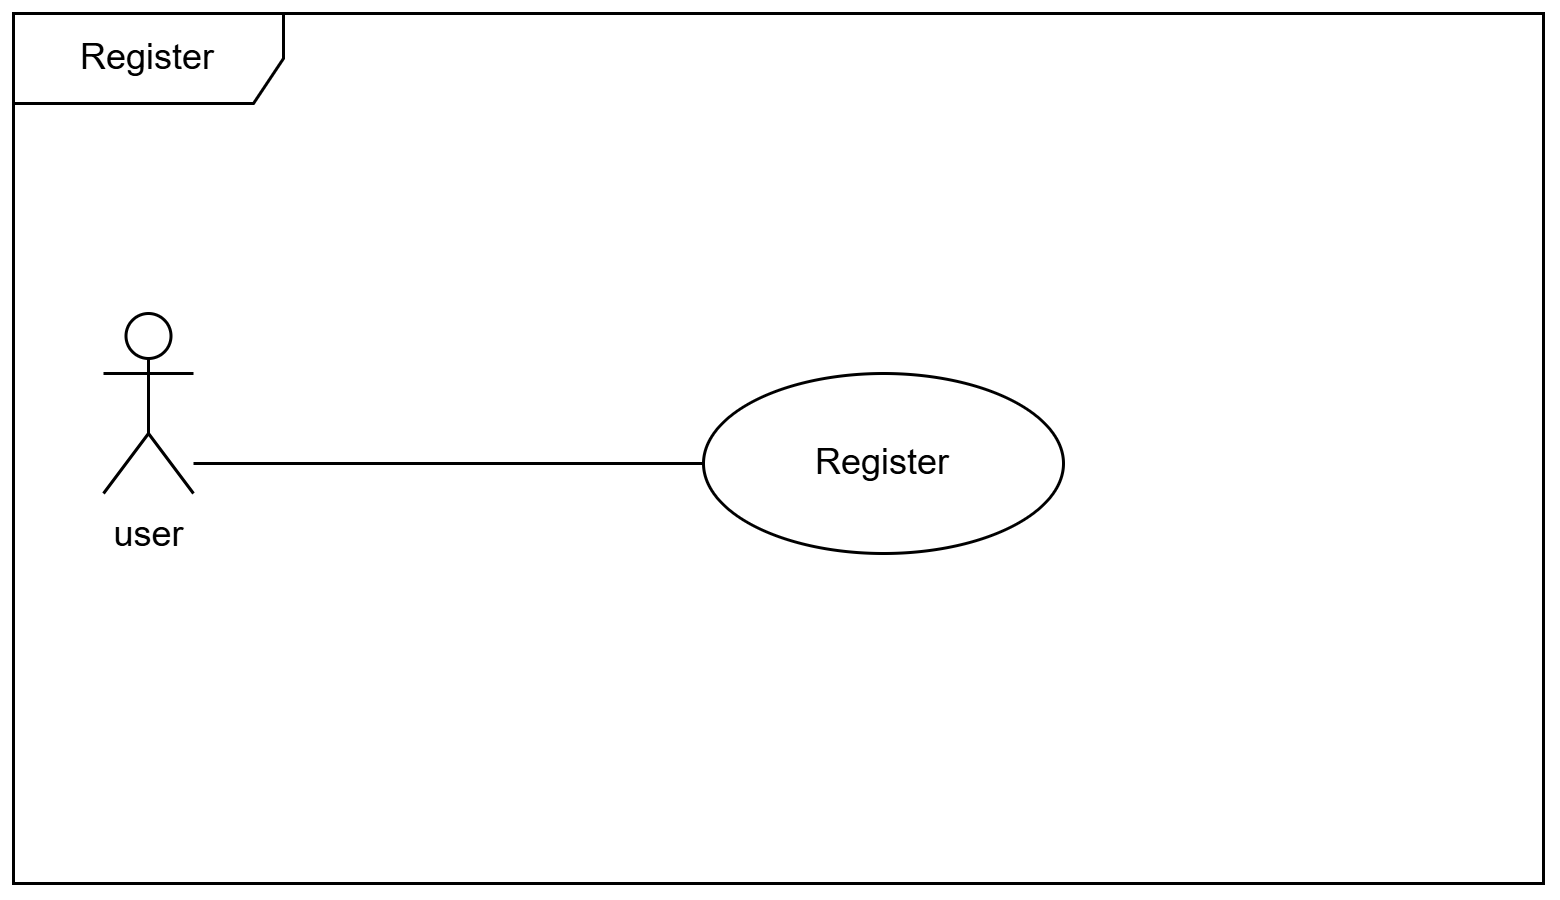
\includegraphics[width=0.8\textwidth]{images/usecase1.drawio.png}
\caption{Use case diagram: Register}
\label{fig:usecase_register}
\end{figure}

\begin{table}[!htbp]
 \centering
 \caption{Textual description of the Register use case}
 \label{tab:register_desc}
 \begin{tabular}{lp{10cm}}
 \toprule
 \textbf{Element} & \textbf{Description} \\
 \midrule
 Use Case & Register \\
 Actor & Visitor (Client / Technician / Company Admin) \\
  Precondition & Visitor opens the registration page. \\
  Postcondition & New profile is created in the database. \\
  Nominal Scenario &
  1. Applicant clicks join. \newline
  2. App renders empty credentials fields. \newline
  3. Applicant fills in email, password, and selects role. \newline
  4. Client sends registration request payload. \newline
  5. Backend hashes password, saves user in MongoDB, and triggers pending status for technicians. \\
 \bottomrule
 \end{tabular}
 \end{table}

\subsubsection{Use Case Refinement: Authenticate}

We secure app access through the login sequence shown in Figure~\ref{fig:usecase_authenticate} and Table~\ref{tab:authenticate_desc}.

\begin{figure}[!htbp]
\centering
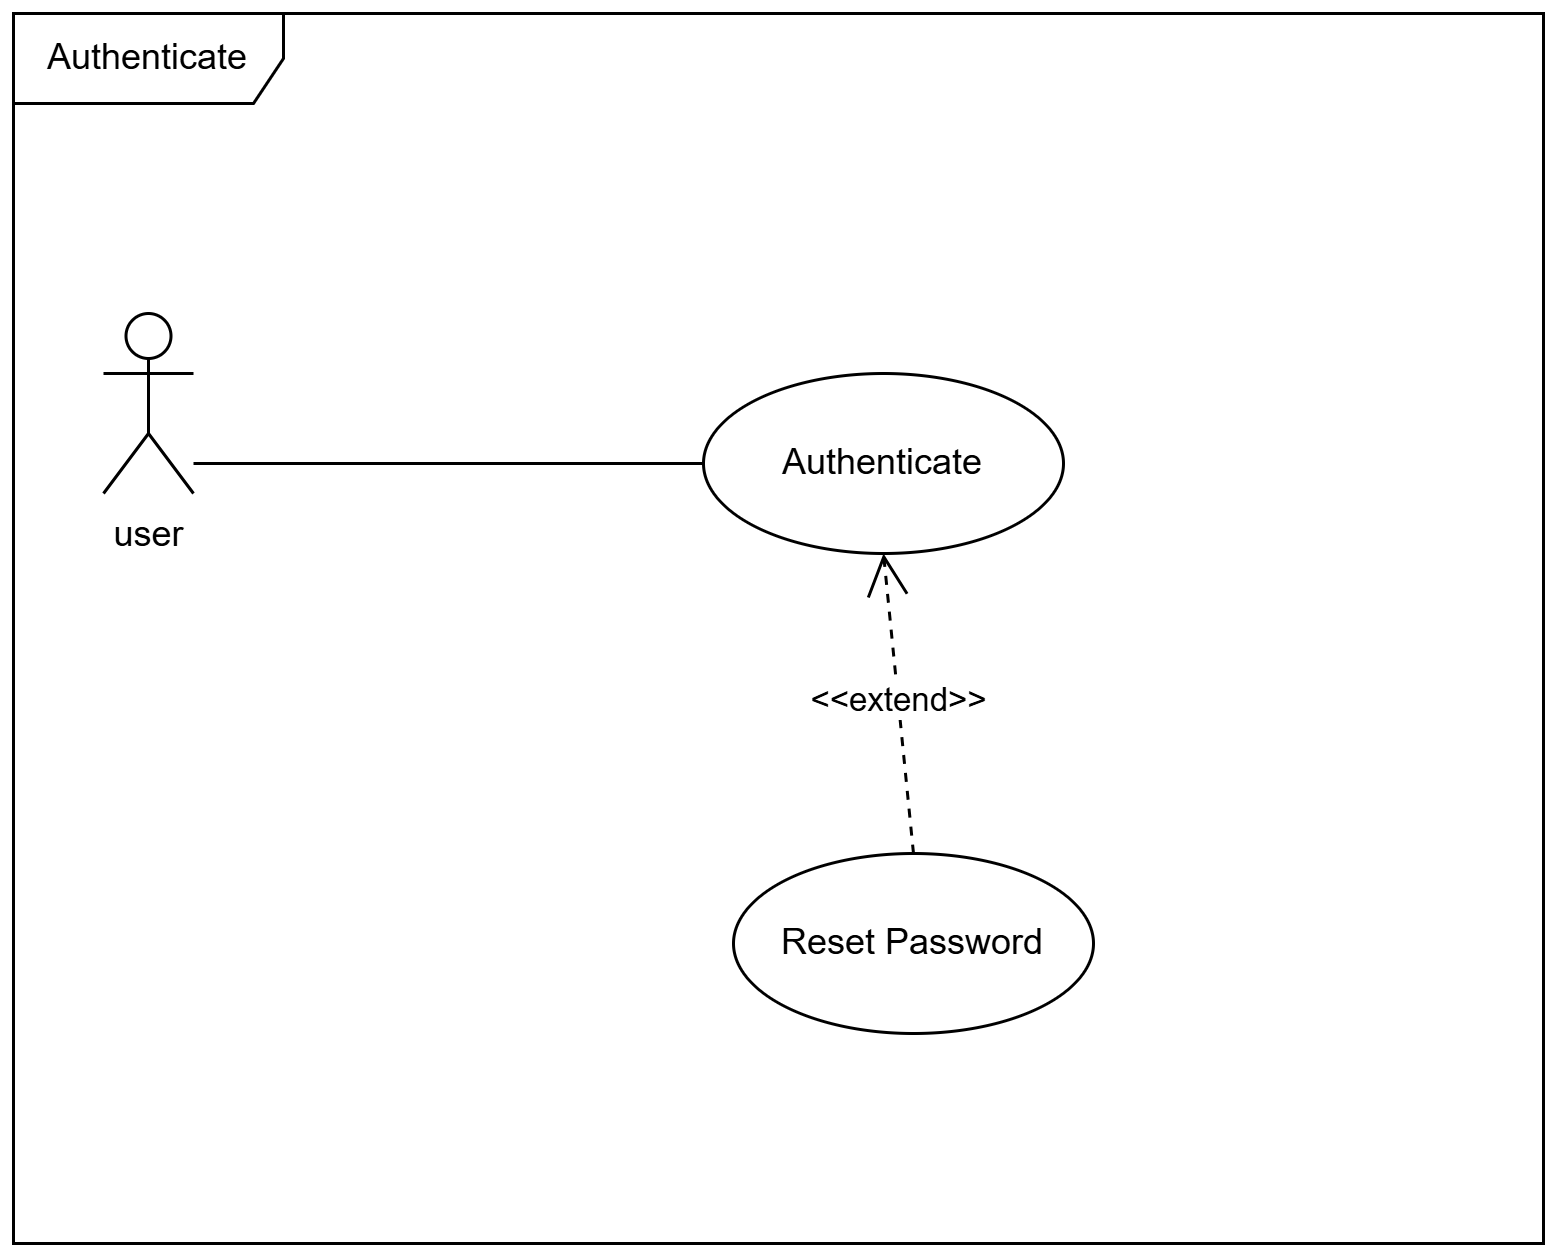
\includegraphics[width=0.8\textwidth]{images/usecase2.drawio.png}
\caption{Use case diagram: Authenticate}
\label{fig:usecase_authenticate}
\end{figure}

\begin{table}[!htbp]
\centering
\caption{Textual description of the Authenticate use case}
\label{tab:authenticate_desc}
\begin{tabular}{lp{10cm}}
\toprule
\textbf{Element} & \textbf{Description} \\
\midrule
Use Case & Authenticate \\
Actor & Client / Technician / Company Admin / Super Admin \\
Precondition & Account document exists in MongoDB. \\
Postcondition & Backend issues active JWT session cookie. \\
Nominal Scenario &
1. User enters email and password. \newline
2. Backend matches bcrypt hash against database record. \newline
3. Server signs JWT token using HS256 algorithm. \newline
4. App stores token in cookie and loads dashboard. \\
\bottomrule
\end{tabular}
\end{table}

\subsubsection{Use Case Refinement: Manage Profile}

Users manage their profiles to keep records accurate. Figure~\ref{fig:usecase_profile} and Table~\ref{tab:profile_desc} show the steps to edit and save personal data.

\begin{figure}[!htbp]
\centering
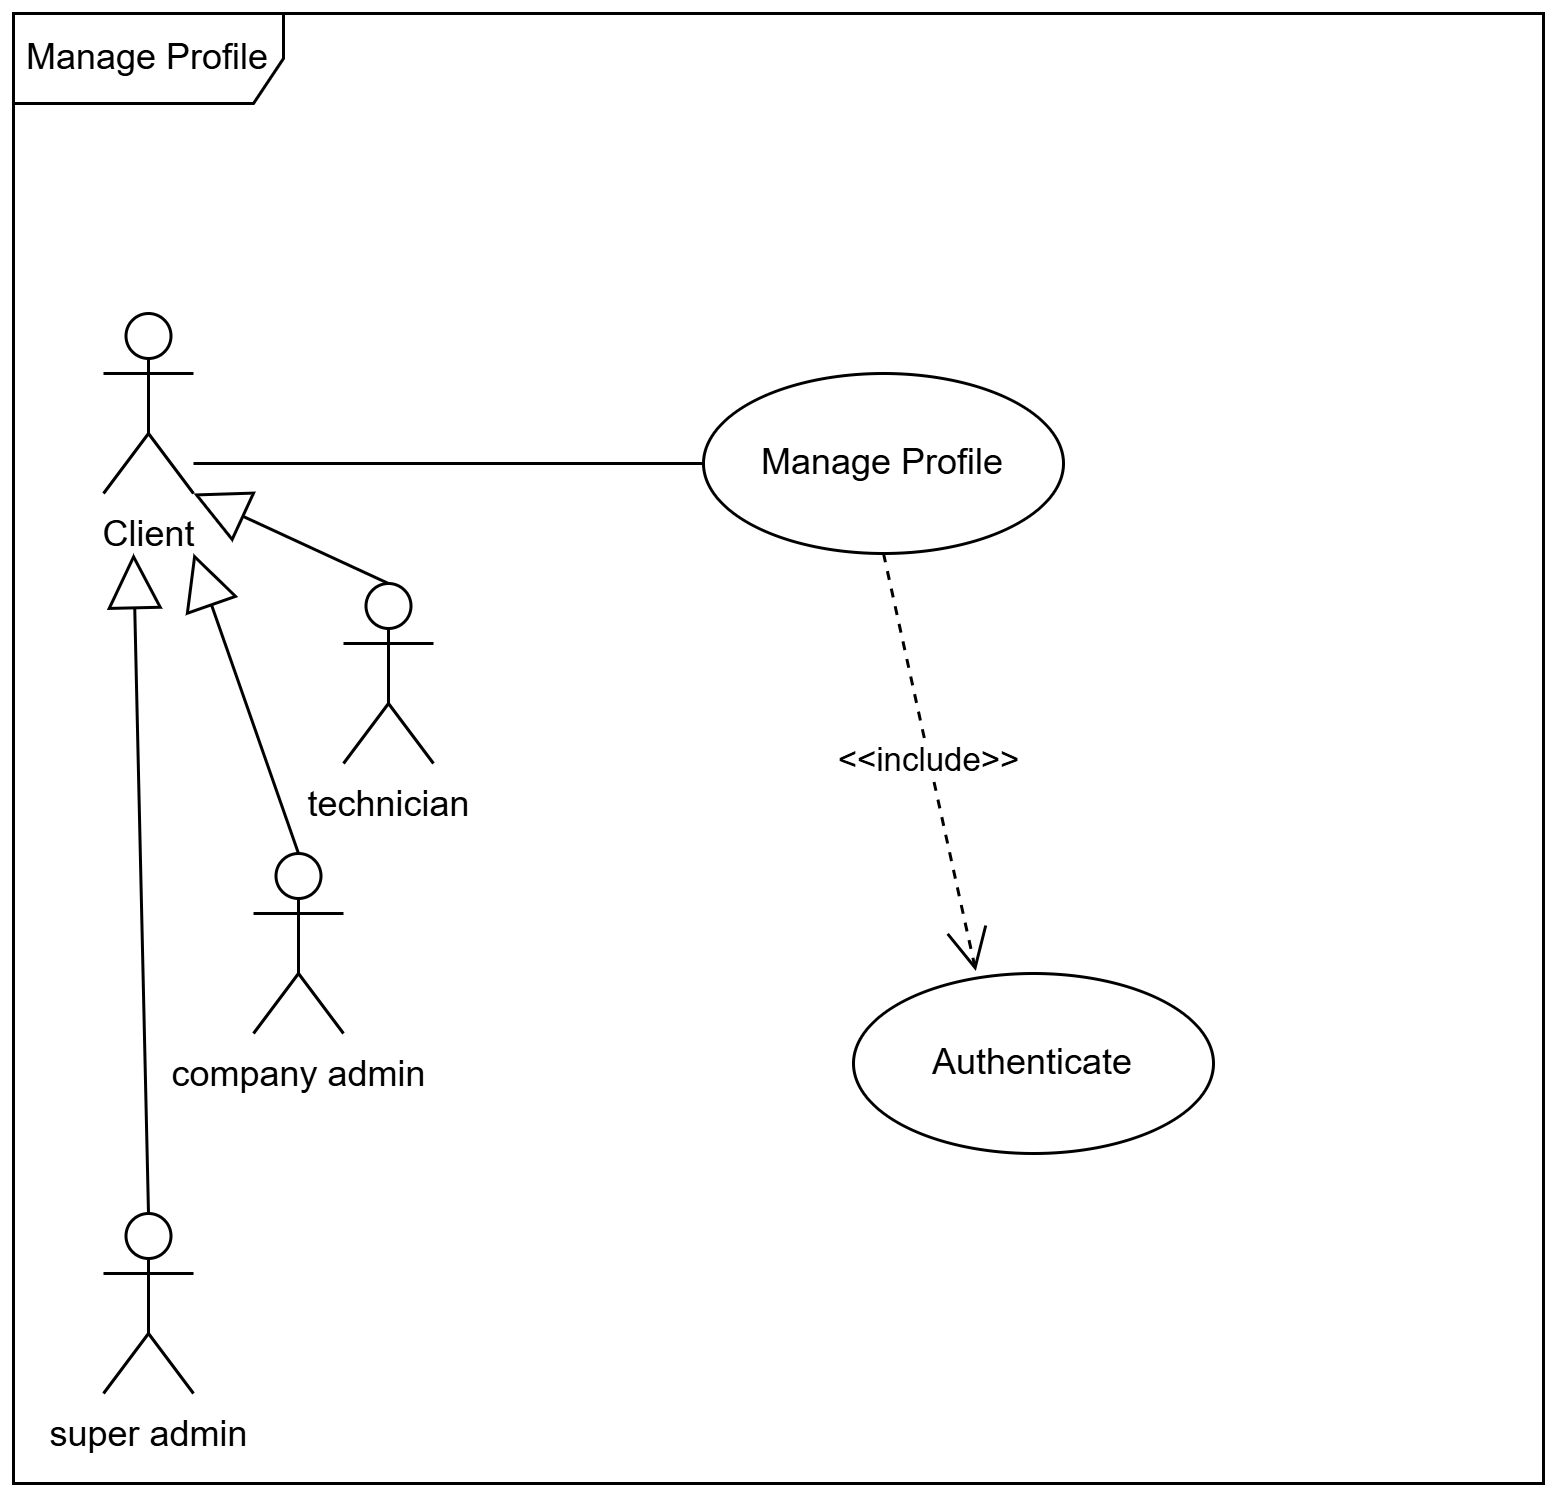
\includegraphics[width=0.8\textwidth]{images/usecase3.drawio.png}
\caption{Use case diagram: Manage Profile}
\label{fig:usecase_profile}
\end{figure}

\begin{table}[!htbp]
\centering
\caption{Textual description of the Manage Profile use case}
\label{tab:profile_desc}
\begin{tabular}{lp{10cm}}
\toprule
\textbf{Element} & \textbf{Description} \\
\midrule
Use Case & Manage Profile \\
Actor & Client / Technician / Company Admin / Super Admin \\
Precondition & Active JWT cookie is present. \\
Postcondition & Database updates the specific user record. \\
Nominal Scenario &
1. User navigates to profile tab. \newline
2. Backend reads user record and returns fields. \newline
3. User edits text inputs. \newline
4. Backend checks fields and updates MongoDB document. \\
\bottomrule
\end{tabular}
\end{table}

\subsection{Class Diagram}

Our user database structure is modeled in the class diagram shown in Figure~\ref{fig:sprint1_class}. We defined a central \texttt{User} entity that handles authentication credentials, linking it to the \texttt{Role} collection to handle permissions dynamically.

\begin{figure}[!htbp]
\centering
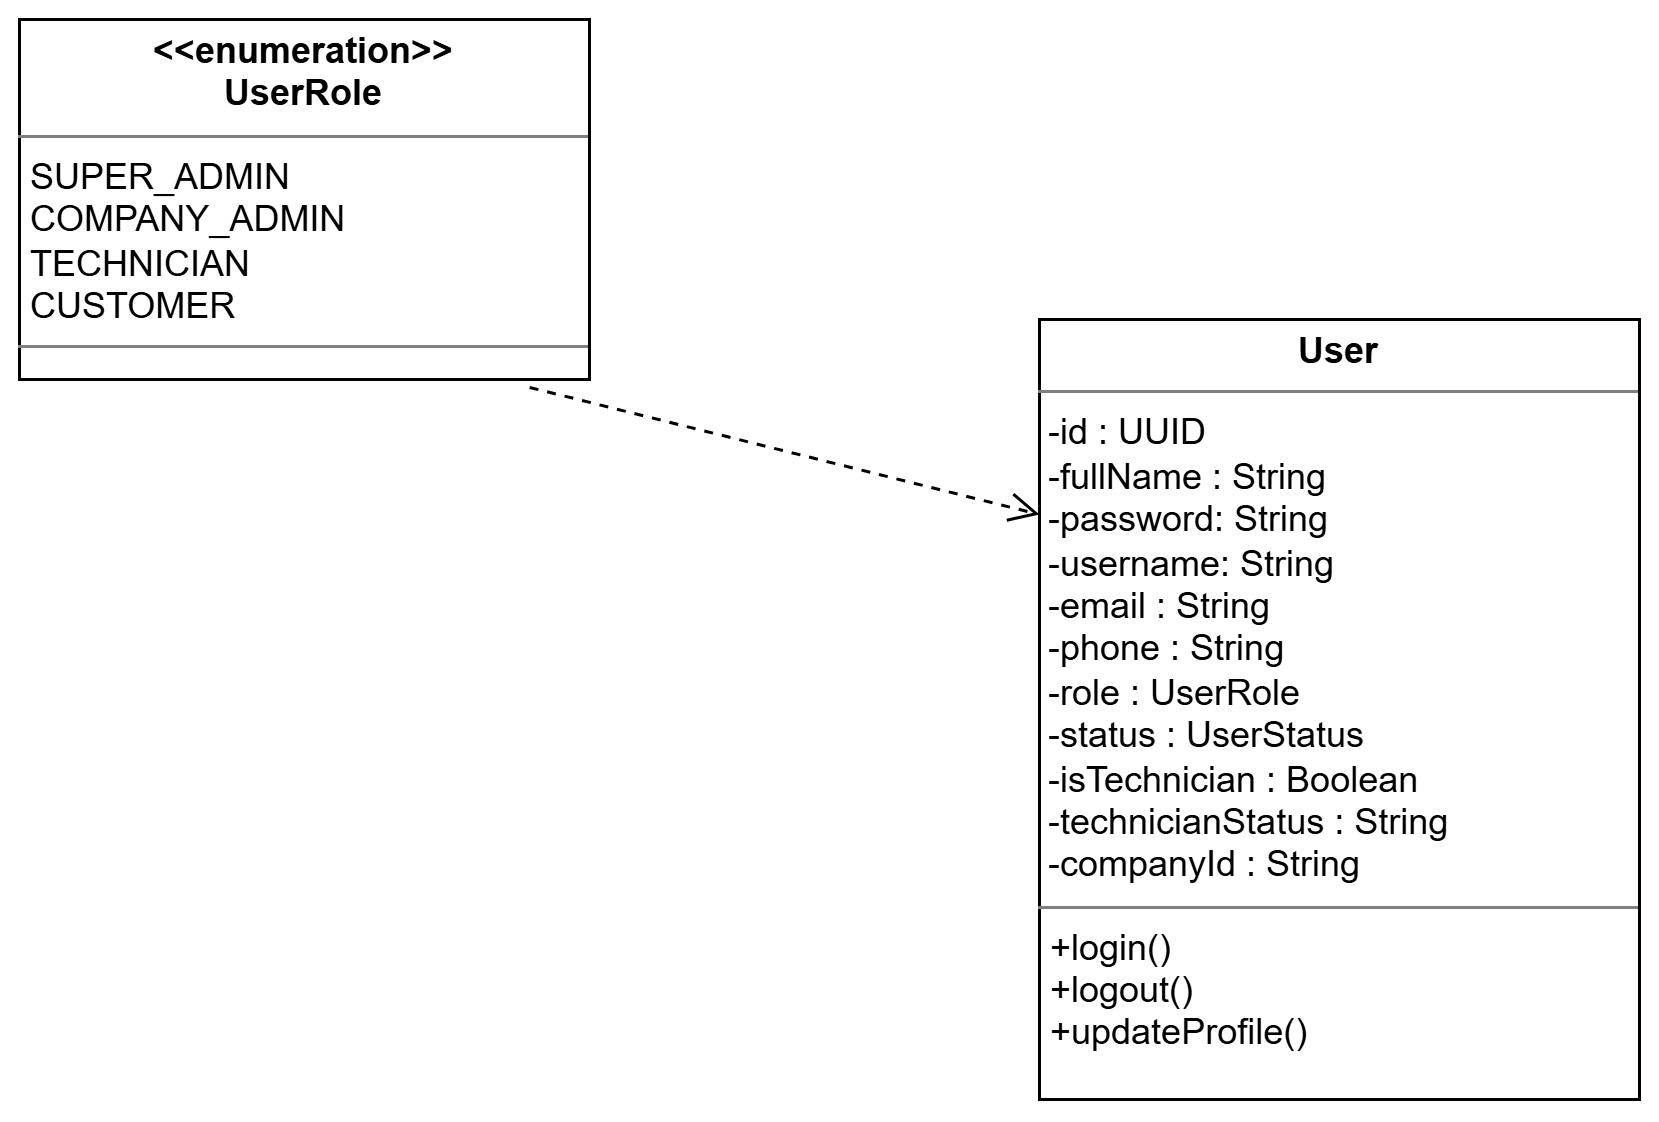
\includegraphics[width=0.9\textwidth]{images/sprint1class1.drawio.png}
\caption{Class diagram – Authentication and user management}
\label{fig:sprint1_class}
\end{figure}

\subsection{Sequence Diagrams}

To visualize how the client app, backend APIs, and database communicate over time, we created sequence diagrams.

\subsubsection{Sequence Diagram: Authentication}

Figure~\ref{fig:seq_auth} traces the message exchange during credential validation and the password recovery flow. It models the dynamic lifecycle interactions between the User, View, Controller, JWT Service, and Database, covering both validation successes and error-handling conditions.

\begin{figure}[!htbp]
 \centering
 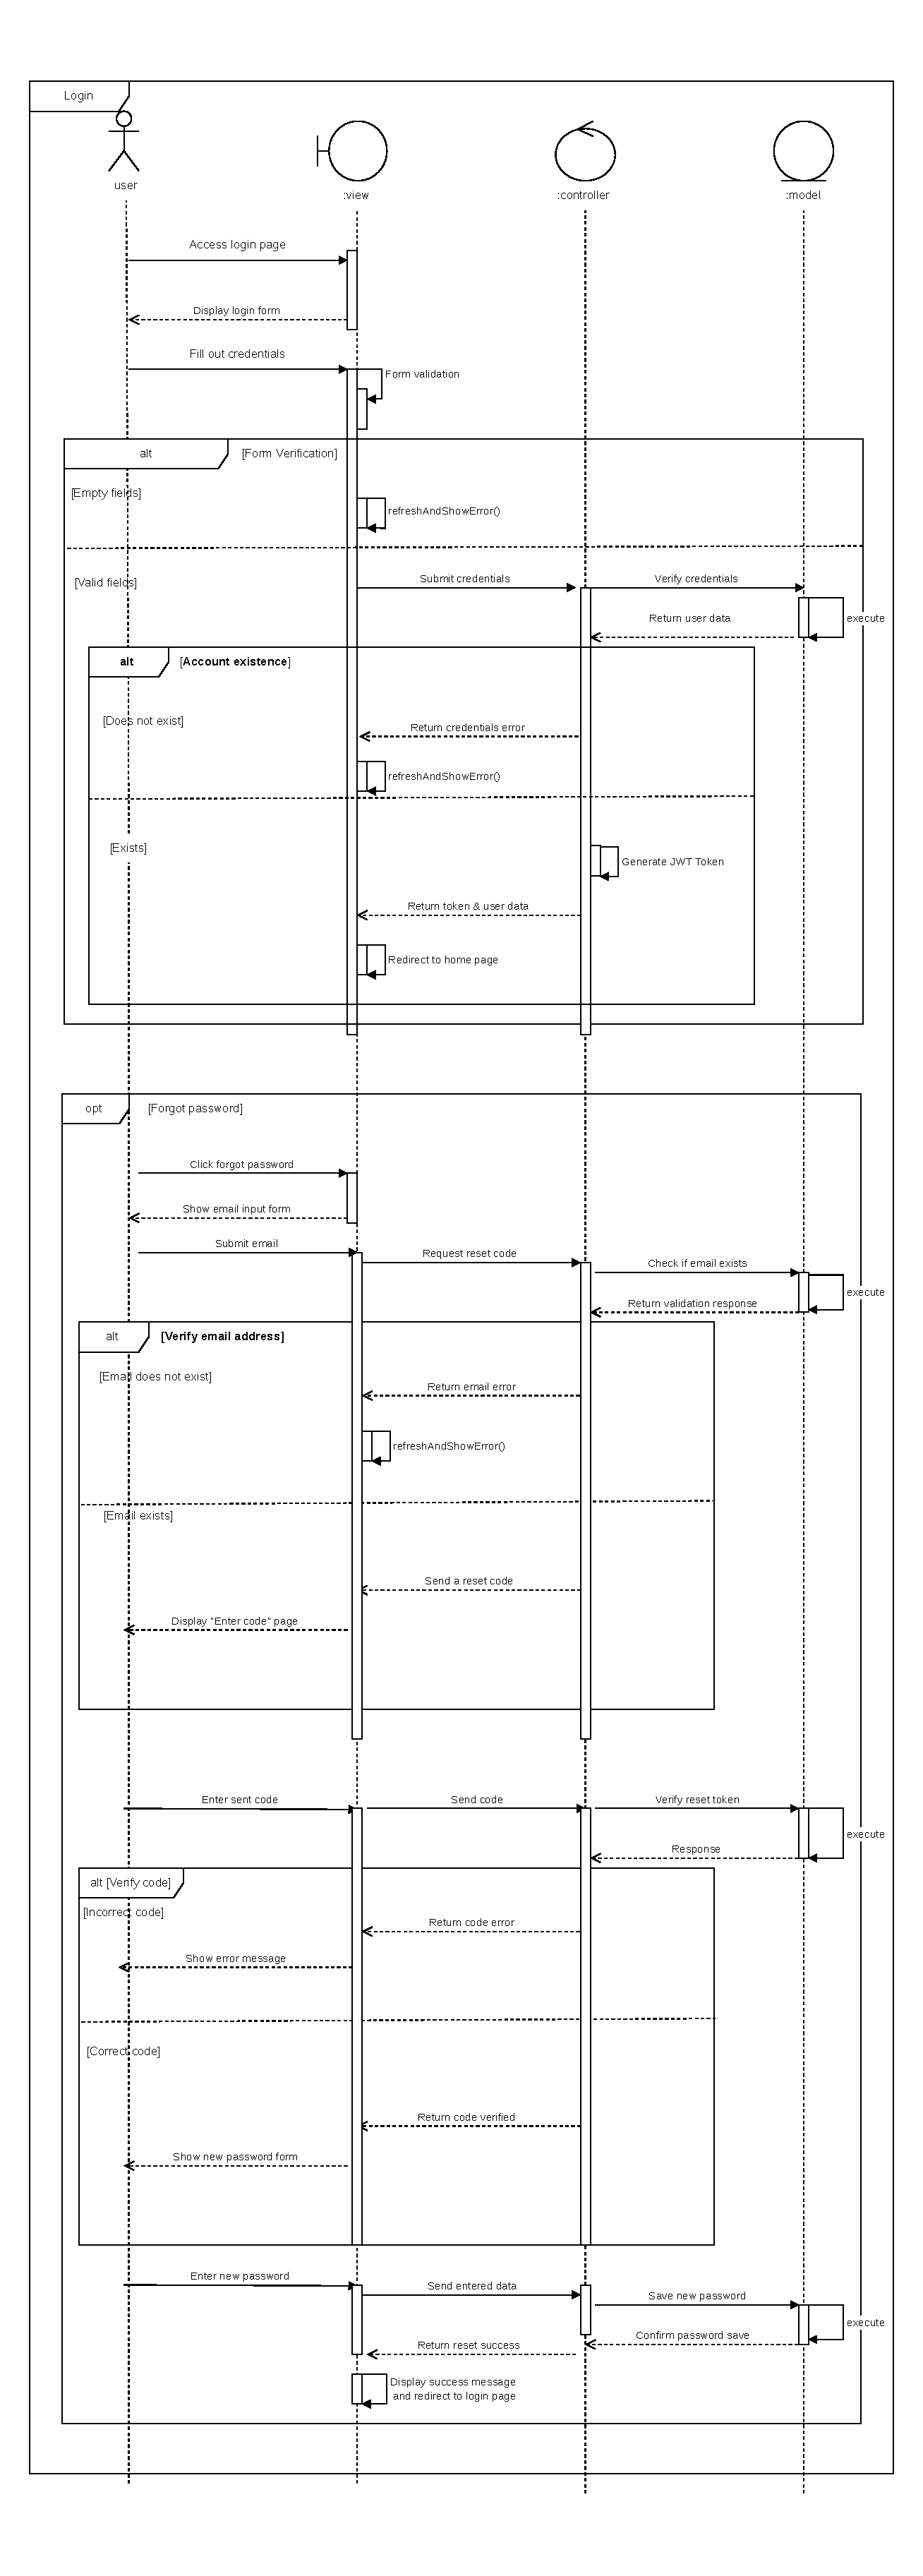
\includegraphics[width=0.9\textwidth]{images/seq1_auth.pdf}
 \caption{Sequence diagram: Authentication process}
 \label{fig:seq_auth}
 \end{figure}
 
 \subsubsection{Sequence Diagram: Profile Management}
 
Figure~\ref{fig:seq_profile} shows how the profile updates travel from the UI to the database.
 
 \begin{figure}[!htbp]
 \centering
 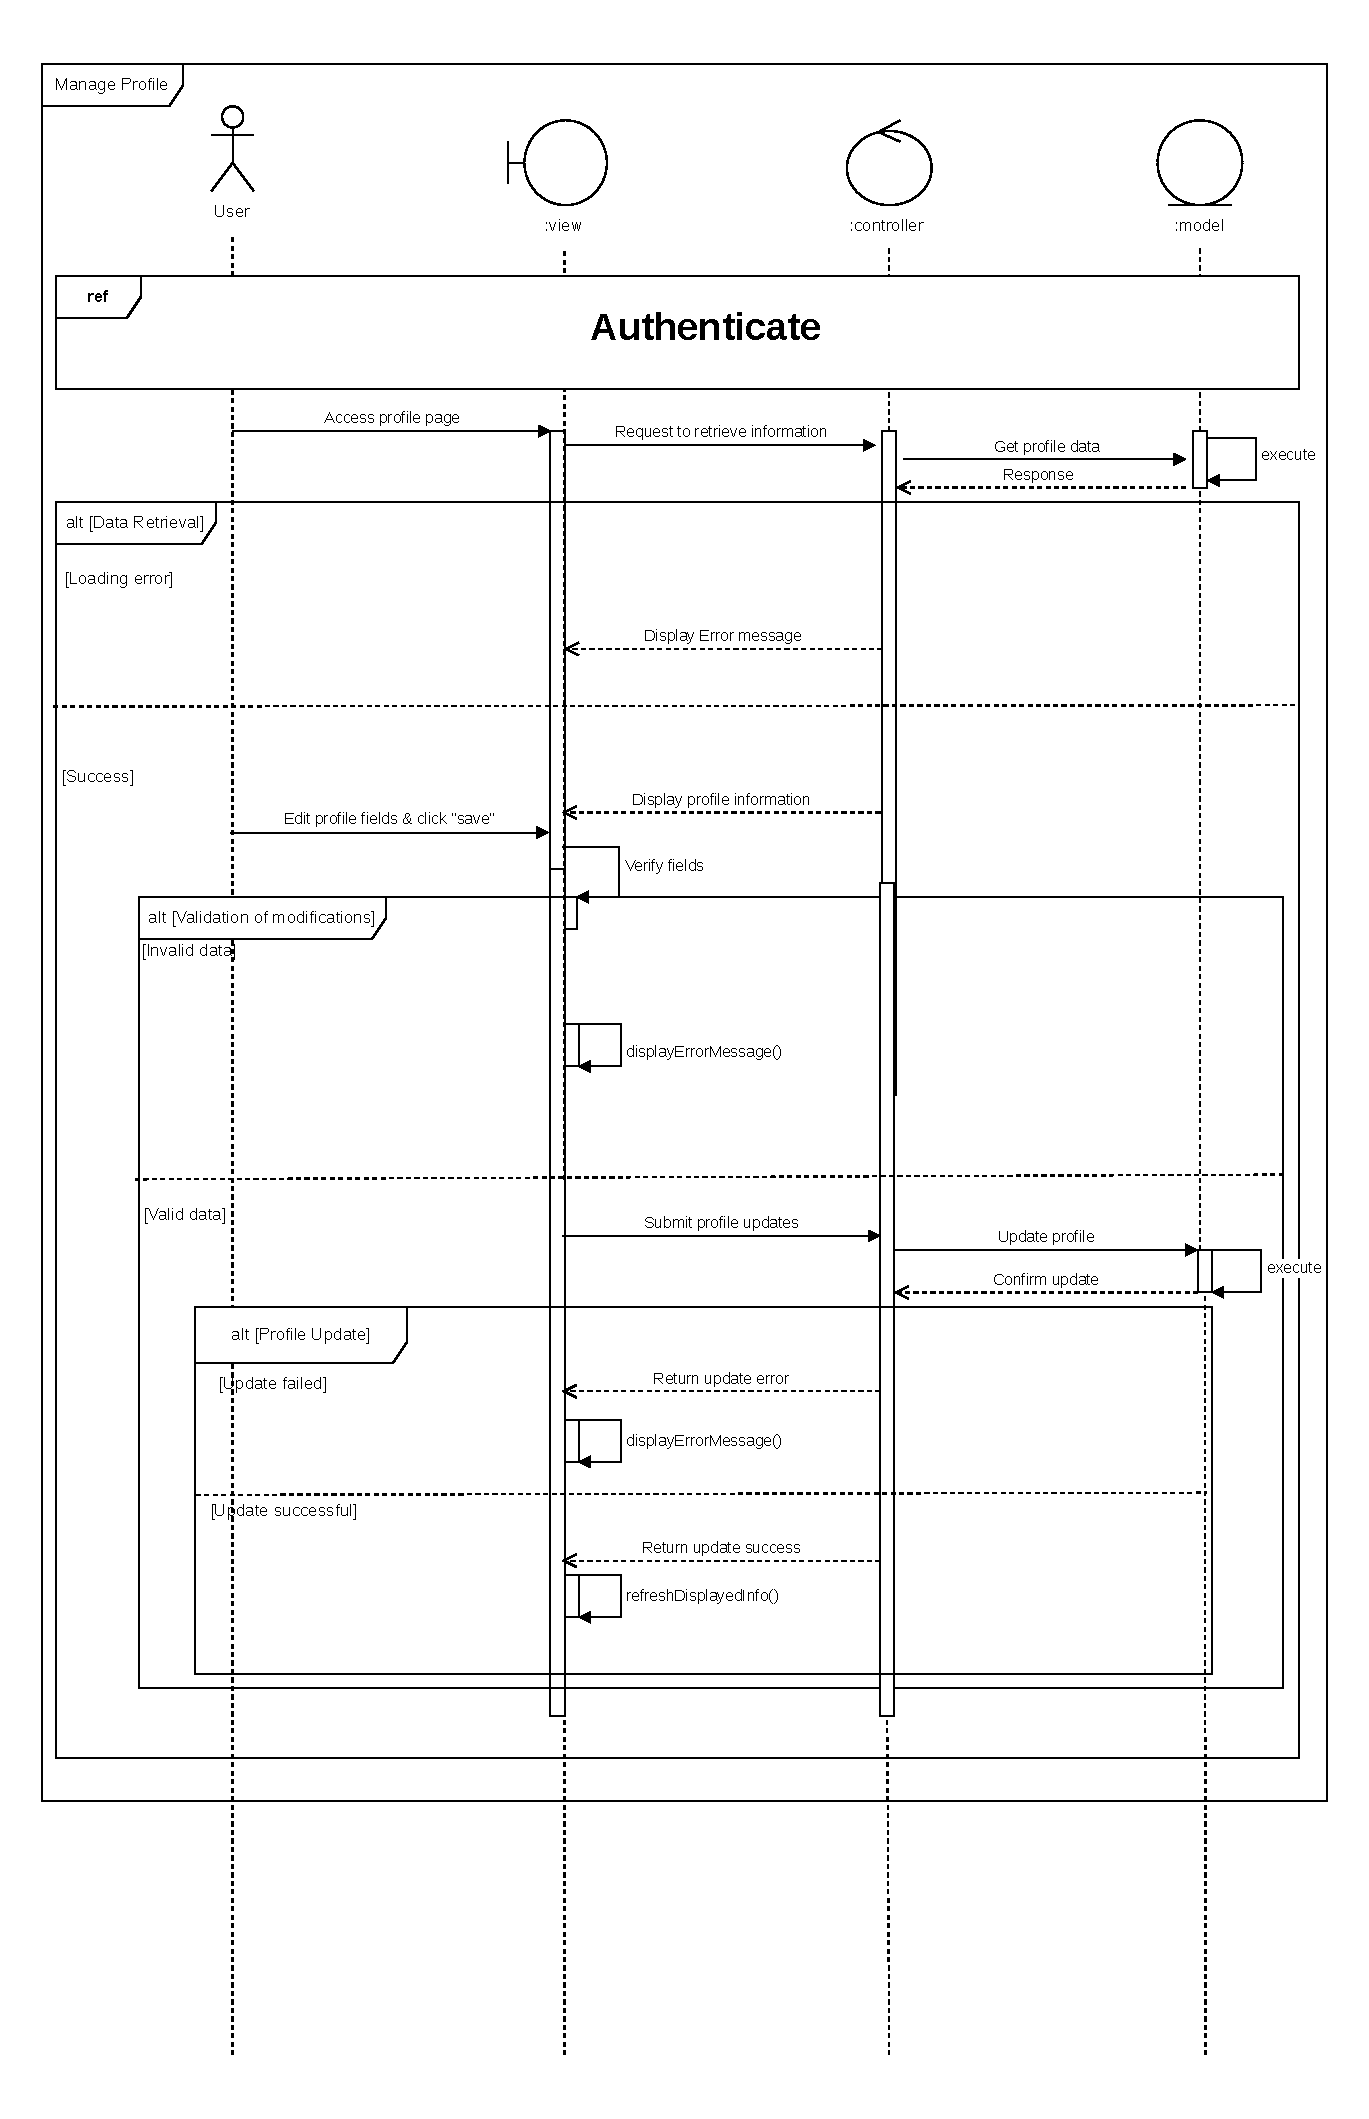
\includegraphics[width=0.9\textwidth]{images/seq2_profile.pdf}
 \caption{Sequence diagram: Profile management}
 \label{fig:seq_profile}
 \end{figure}
 
 \section{User Interface Overview}
 
Here, we showcase the actual web and mobile interfaces we implemented for this release.
 
 \subsection{Web Application Interfaces}
 
We built the web portal to serve admins, clients, and technicians. We used modern web tools to ensure fast loading and responsive pages.
 
 \subsubsection{Authentication Interfaces}
 
We designed the registration and login pages to offer clean forms and quick Google social login.
 
 \begin{figure}[!htbp]
 \centering
 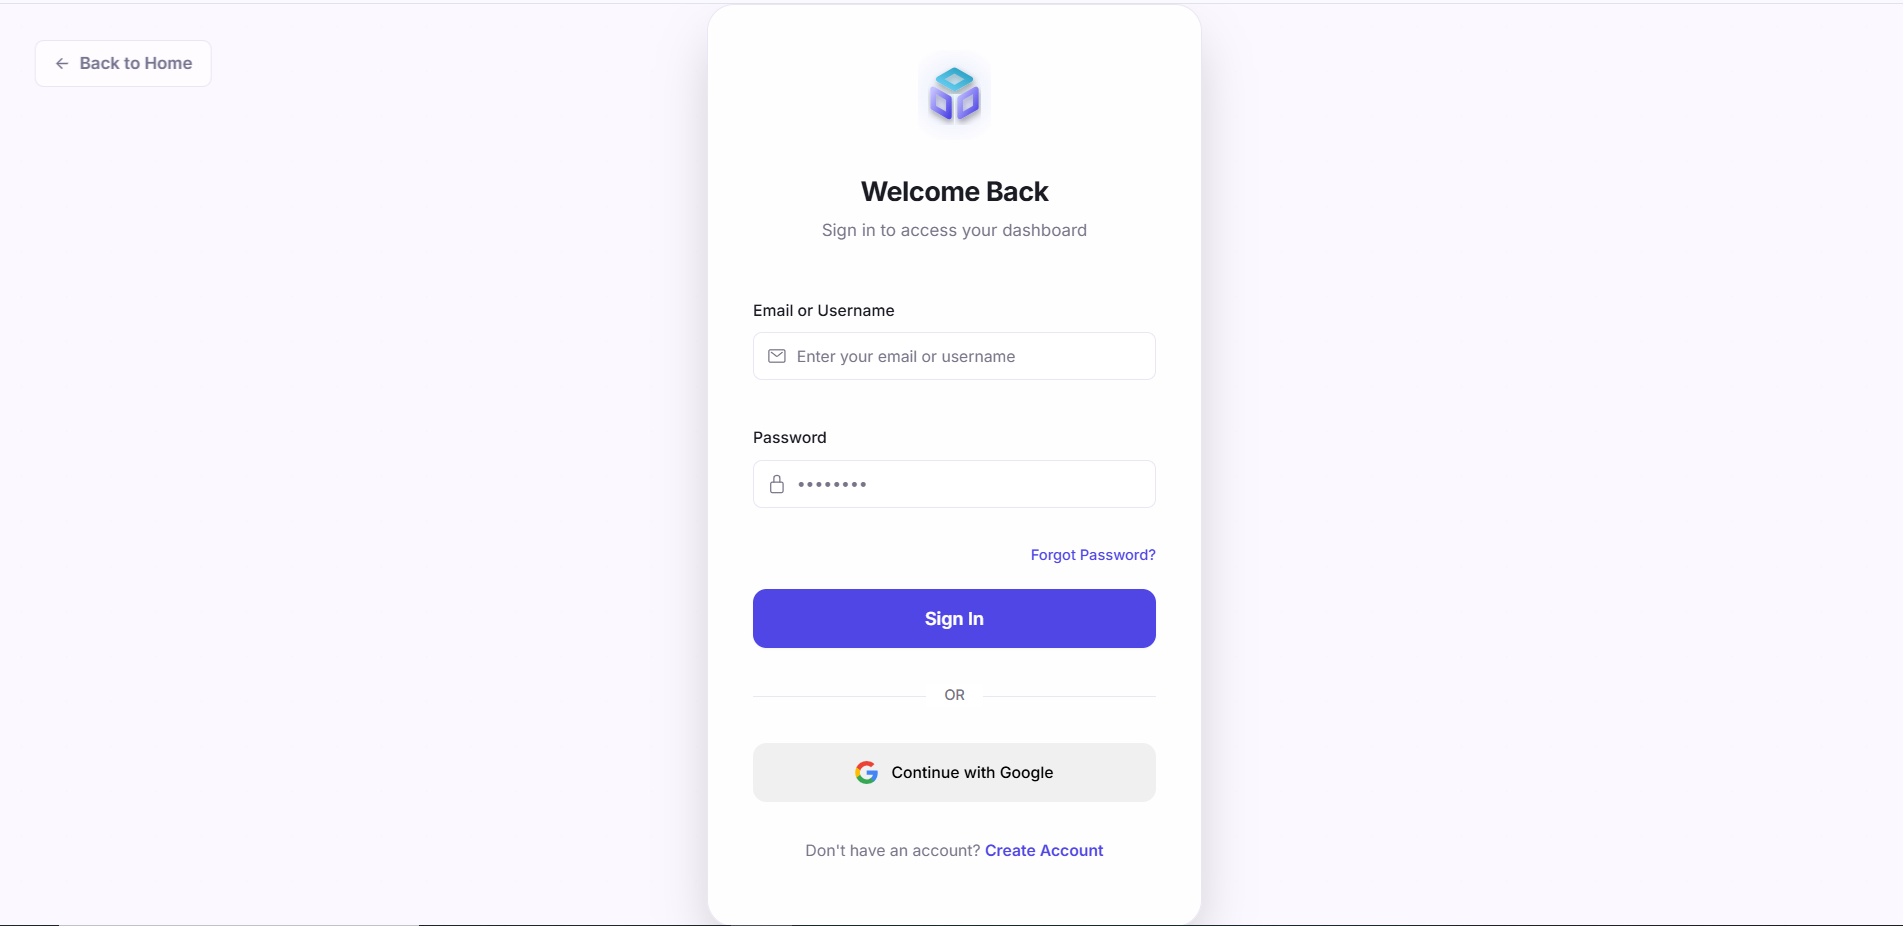
\includegraphics[width=0.45\textwidth]{images/login.PNG}
 \hfill
 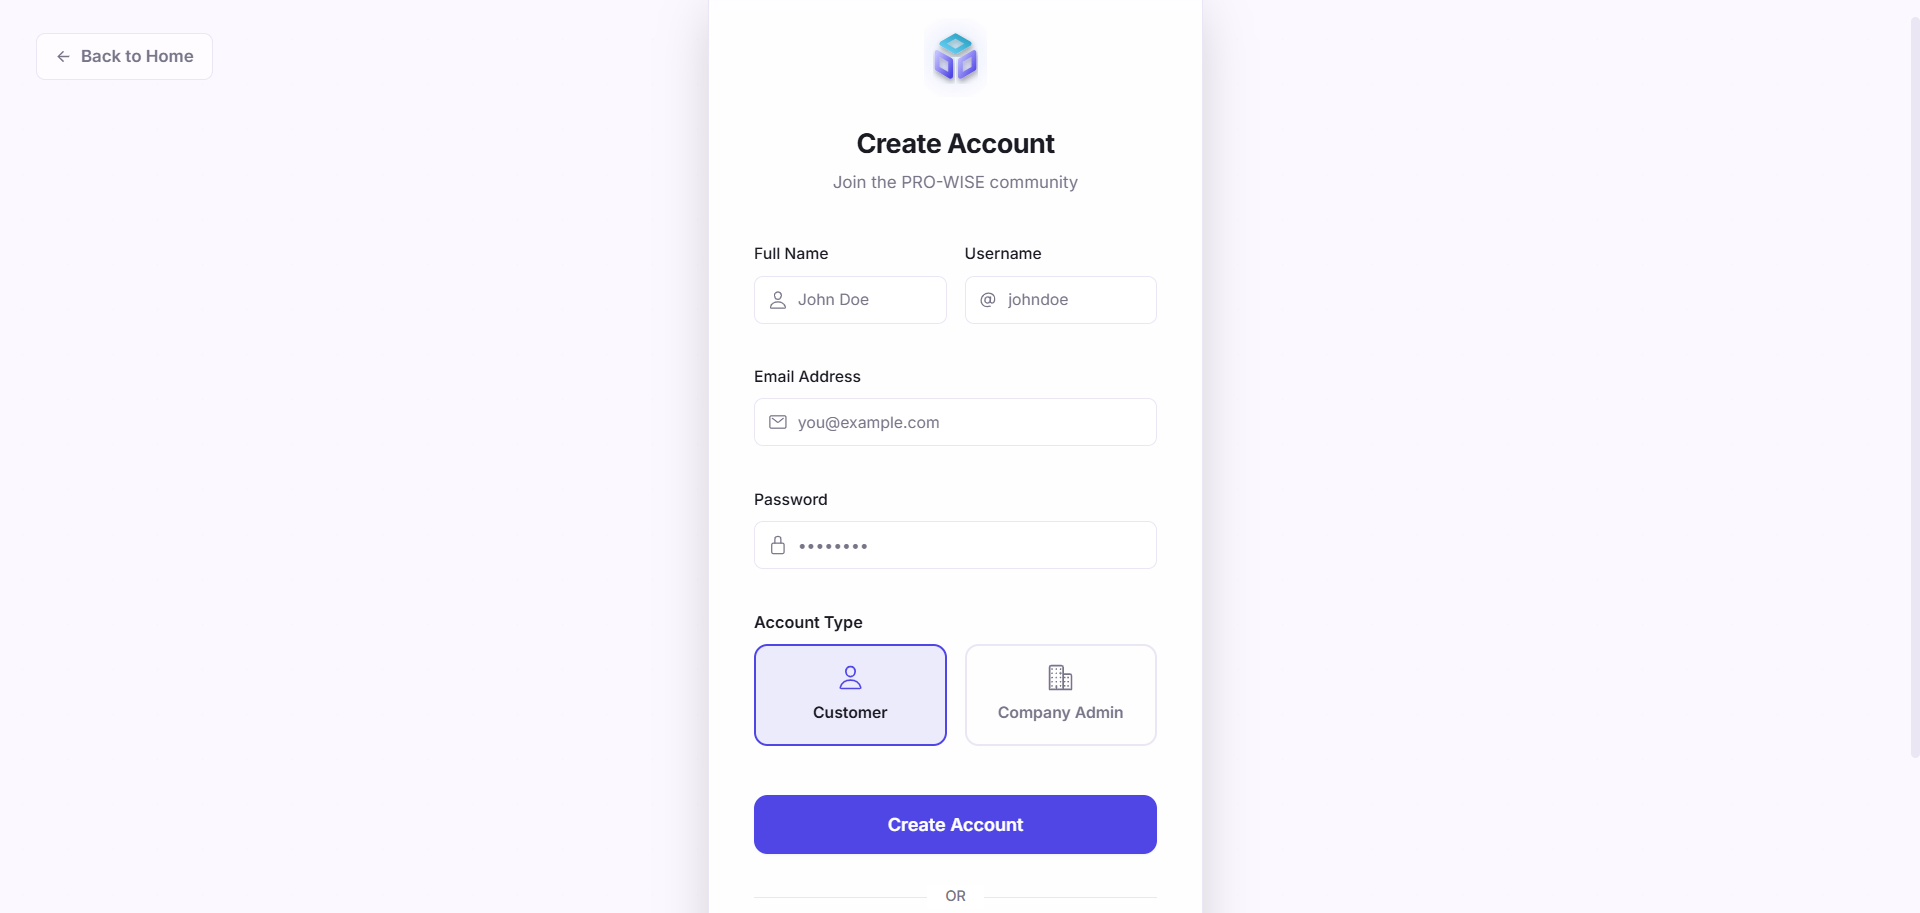
\includegraphics[width=0.45\textwidth]{images/Register.PNG}
 \caption{Web interfaces – Login and Registration pages}
 \label{fig:web_auth}
 \end{figure}
 
 We designed these forms to be quick to fill out while keeping credentials secure.
 
 \subsubsection{Dashboard and Navigation}
 
Once logged in, users see a custom dashboard. Figure~\ref{fig:web_dashboard} shows the main layout.
 
 \begin{figure}[!htbp]
 \centering
 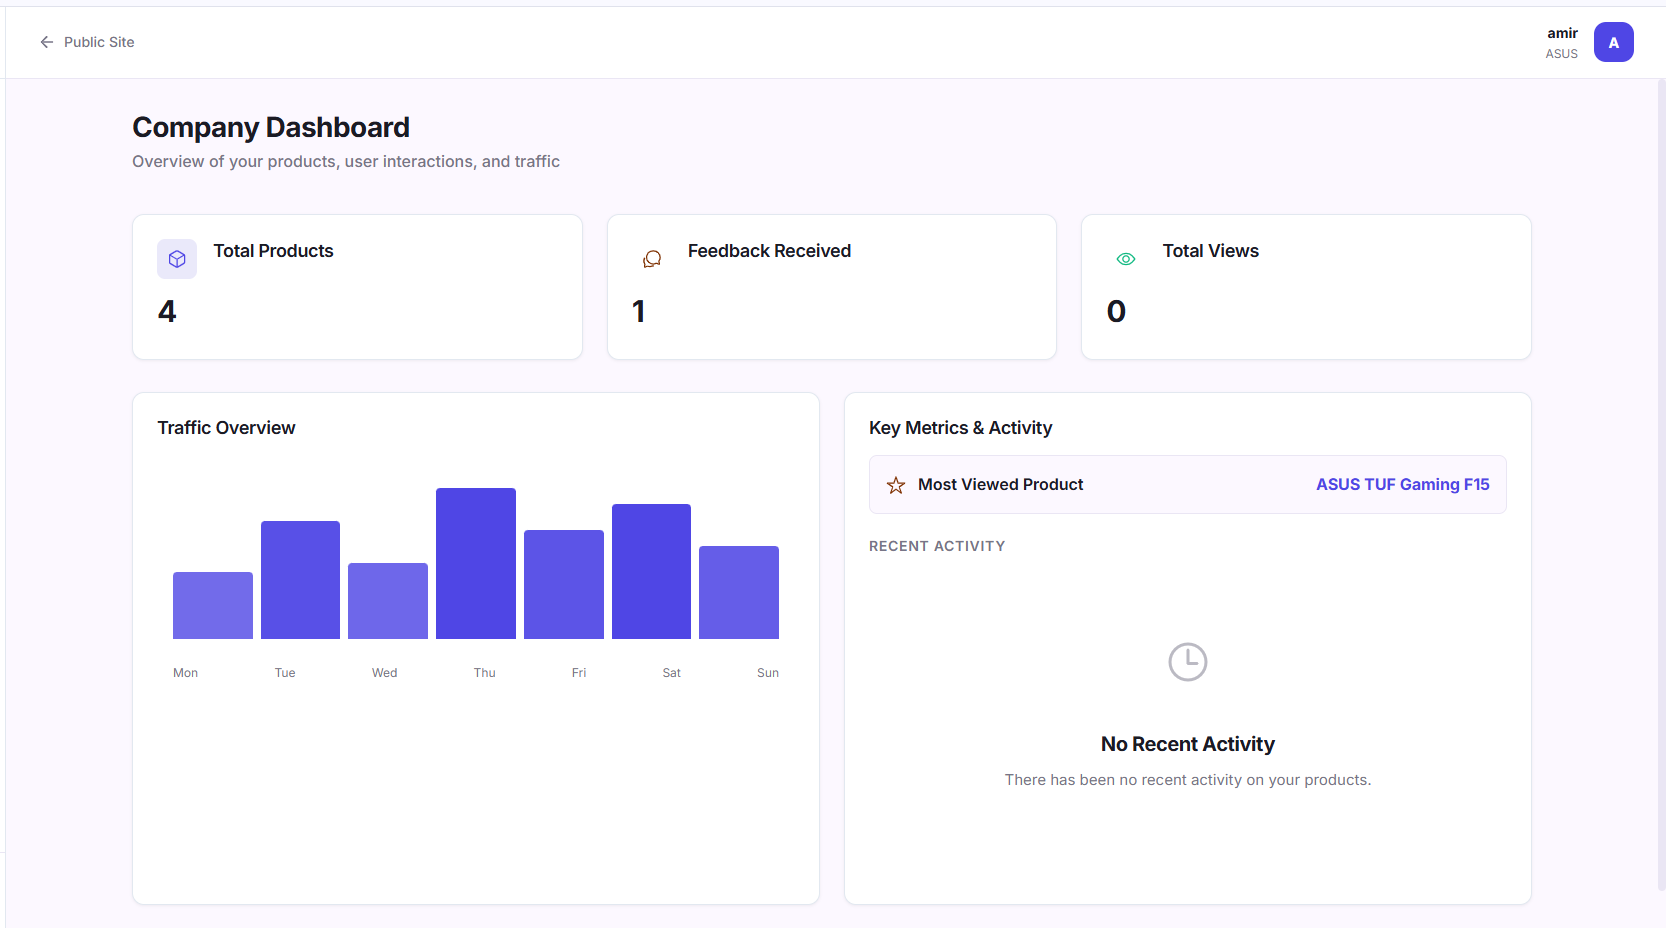
\includegraphics[width=0.9\textwidth]{images/dashbord.PNG}
 \caption{Web interface – User dashboard}
 \label{fig:web_dashboard}
 \end{figure}
 
 This layout gives users a single starting point to reach any tool on the platform.
 
 \subsubsection{Profile Management Interface}
 
We created the profile section in Figure~\ref{fig:web_profile} to allow technicians to upload their verification files.
 
 \begin{figure}[!htbp]
 \centering
 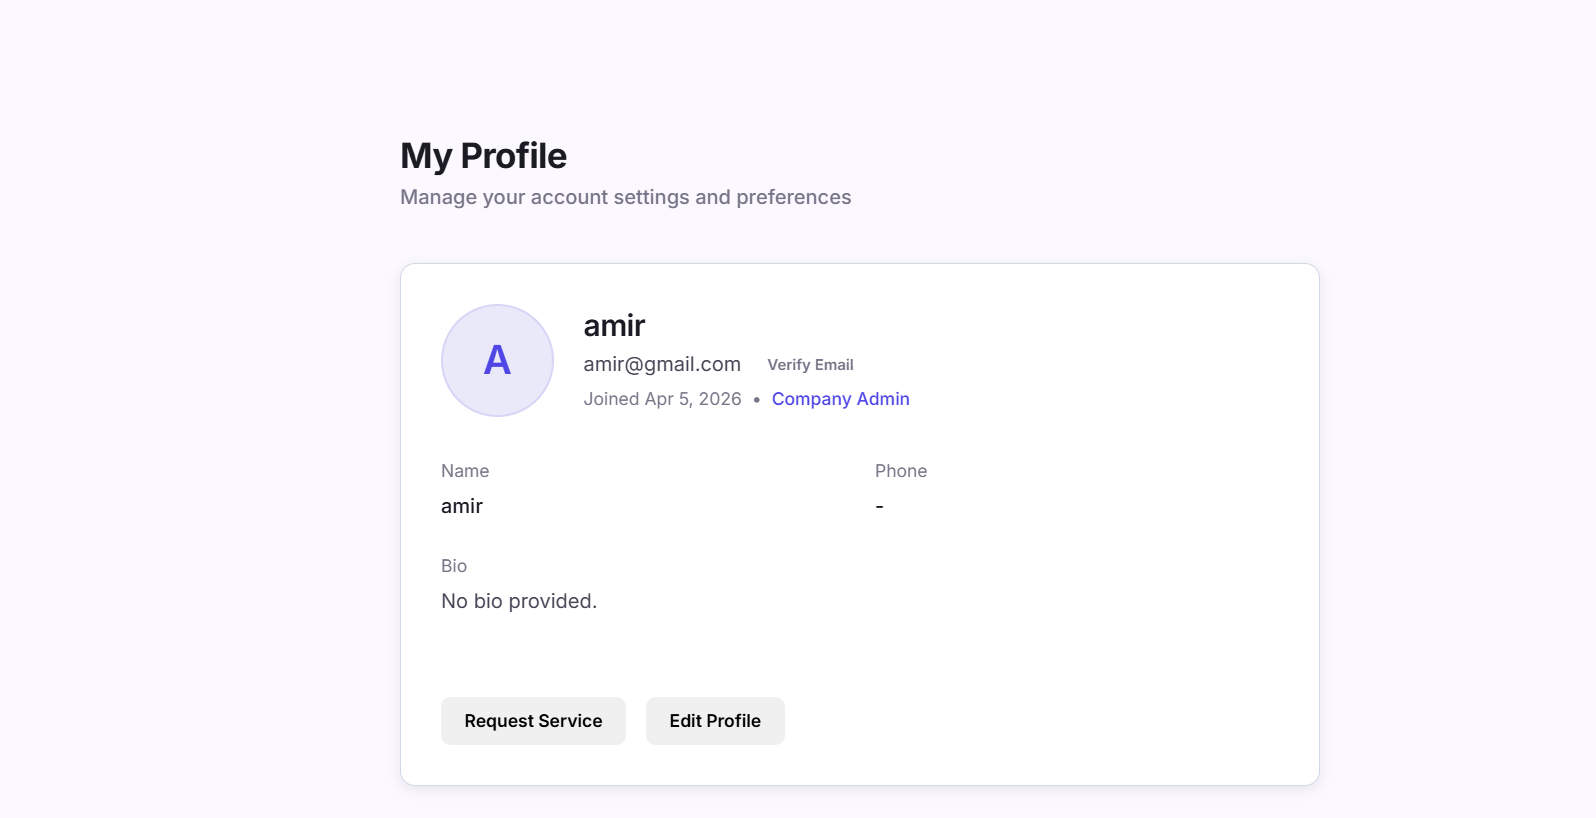
\includegraphics[width=0.9\textwidth]{images/Profile managment.PNG}
 \caption{Web interface – Profile management}
 \label{fig:web_profile}
 \end{figure}
 
 This screen makes it easy for technicians to keep their qualifications up to date.
 
 \subsection{Mobile Application Interfaces}
 
We also built a cross-platform mobile app using React Native and Expo to help technicians update data while on-site.
 
 \subsubsection{Authentication Screens}
 
Our mobile login and registration screens feature a simplified, single-column layout adapted to touch interactions.
 
 \begin{figure}[!htbp]
 \centering
 \includegraphics[width=0.4\textwidth]{images/mobile_login.png}
 \hfill
 \includegraphics[width=0.4\textwidth]{images/mobile_register.png}
 \caption{Mobile interfaces – Login and Registration screens}
 \label{fig:mobile_auth}
 \end{figure}
 
 \subsubsection{Home and Navigation}
 
The home screen acts as a dashboard shortcut panel for key features.
 
 \begin{figure}[!htbp]
 \centering
 \includegraphics[width=0.4\textwidth]{images/mobile_home.png}
 \caption{Mobile interface – Home screen}
 \label{fig:mobile_home}
 \end{figure}
 
 We designed the navigation to feel snappy and natural on mobile screens.
 
 \subsubsection{Profile Interface}
 
Technicians use the profile view in Figure~\ref{fig:mobile_profile} to manage credentials on the go.
 
 \begin{figure}[!htbp]
 \centering
 \includegraphics[width=0.4\textwidth]{images/mobile_profile.png}
 \caption{Mobile interface – Profile management}
 \label{fig:mobile_profile}
 \end{figure}
 
 This allows users to update their details on the spot, keeping the backend data fresh.
 
 \section{Conclusion}
 
With this authentication and user management foundation complete, we can implement catalog browsing and content moderation.

\chapter{Release 2 : Product Management, Guides, and Content approval}

\section{Introduction}

This chapter covers the creation of our catalog manager, guide editors, and content review queues. For Release 2, we focused on enabling brand administrators and technicians to publish structured manual pages and link them directly to products.

We structured this release around four main goals:
\begin{itemize}
    \item \textbf{Product Catalog Management}: We built tools for company administrators to structure categories and product models under their brand.
    \item \textbf{Structured Troubleshooting Guides}: We created a guide editor where experts can write detailed steps with text, images, and videos.
    \item \textbf{Hardware-to-Digital Mapping}: We linked physical hardware to digital manuals through product-specific QR codes.
    \item \textbf{Content Approval Pipeline}: We implemented a draft review workflow so that all manuals are validated before going live.
\end{itemize}

\section{Sprint Backlog -- Content and Catalog Management}

The user stories selected for this catalog sprint are listed in Table~\ref{tab:sprint2_backlog}, detailing their priorities and functional requirements.

\renewcommand{\arraystretch}{1.3}
\setlength{\tabcolsep}{8pt}

\begin{table}[!htbp]
\centering
\caption{User stories for Release 2 (Content and Catalog Management)}
\label{tab:sprint2_backlog}
\resizebox{\textwidth}{!}{%
\begin{tabular}{clp{8cm}c}
\toprule
\textbf{ID} & \textbf{Feature / Epic} & \textbf{Description} & \textbf{Priority} \\
\midrule
4 & Category Management & Management of predefined product categories & High \\
6 & Product Management & CRUD operations for products linked to companies & High \\
8 & Product Details Page & Display of product information, guides, and media & High \\
9 & Guide Management & Creation of structured guides with step-by-step instructions & High \\
10 & Media Support & Upload and management of PDFs, videos, and images & High \\
11 & Content Approval System & Validation workflow for content publication & High \\
\bottomrule
\end{tabular}%
}
\end{table}

\section{Refinement of Use Cases}

We refined three core use cases for the catalog sprint to structure our database collections and policy controllers. These outline the step-by-step nominal paths for catalog managers.

\subsection{Refinement of Sprint 2 Use Cases}

\subsubsection{Use Case Refinement: Manage Products}

Company administrators use the product management module to update their catalog. Figure~\ref{fig:usecase_manage_products} and Table~\ref{tab:manage_products_desc} detail this CRUD flow.

\begin{figure}[!htbp]
\centering
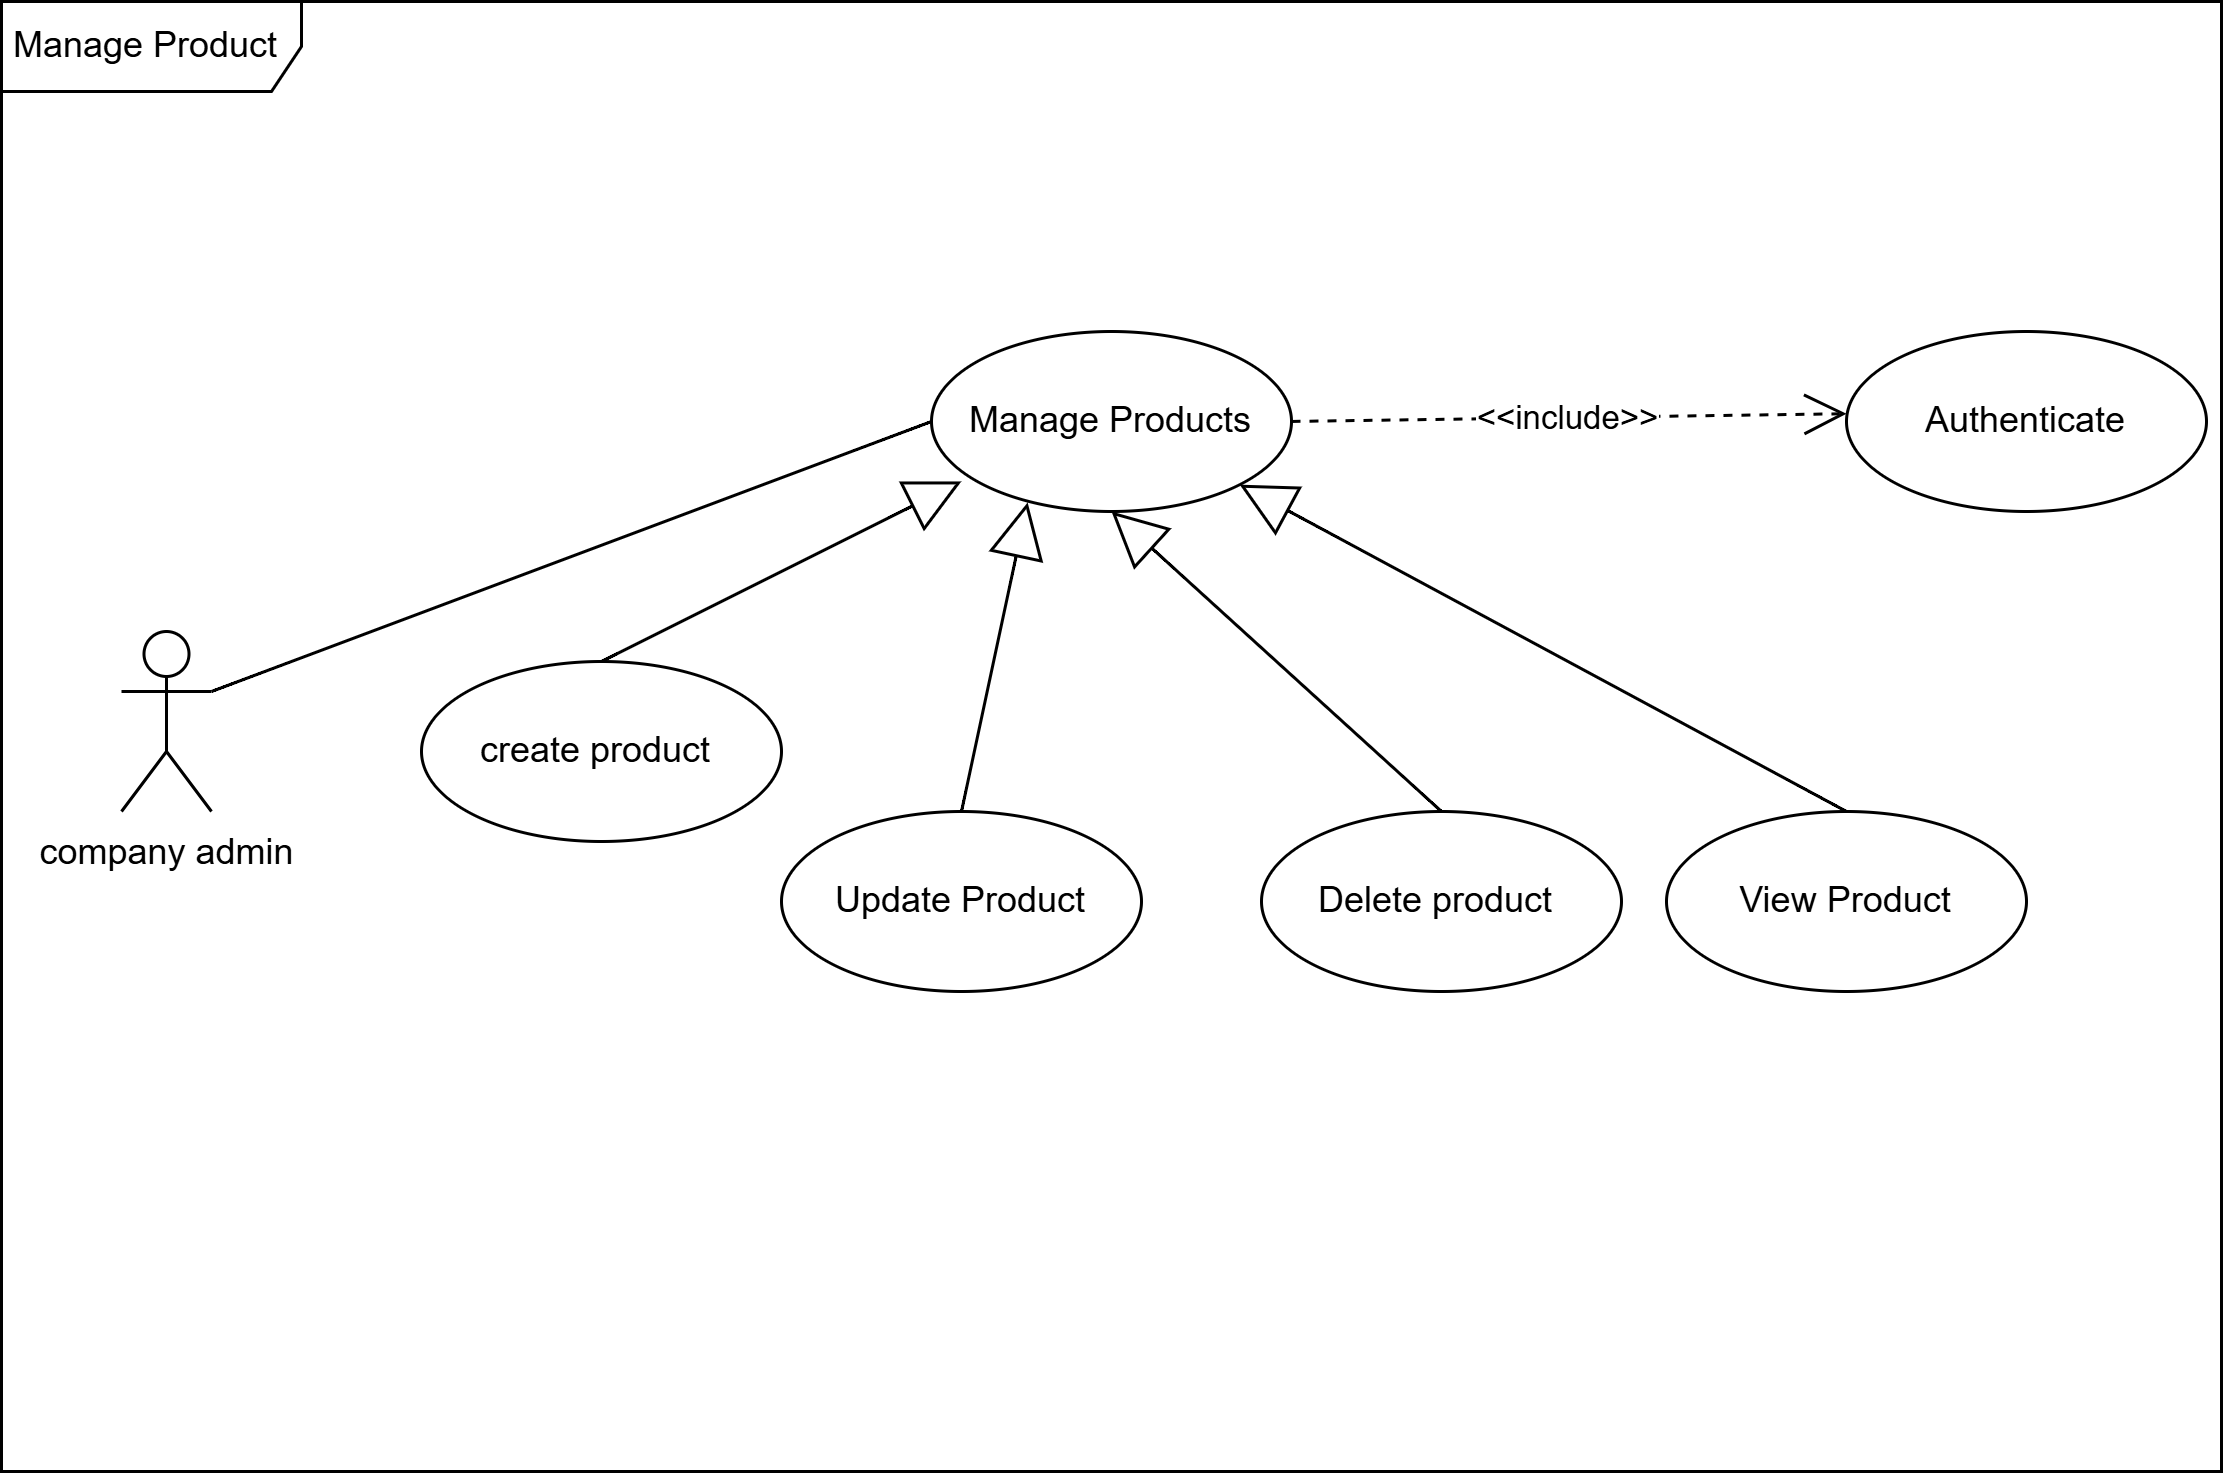
\includegraphics[width=0.8\textwidth]{images/usecase4.drawio.png}
\caption{Use case diagram: Manage Products}
\label{fig:usecase_manage_products}
\end{figure}

\begin{table}[!htbp]
\centering
\caption{Textual description of the Manage Products use case}
\label{tab:manage_products_desc}
\begin{tabular}{lp{10cm}}
\toprule
\textbf{Element} & \textbf{Description} \\
\midrule
Use Case & Manage Products \\
Actor & Company Admin \\
Precondition & Admin session is active with valid brand ID. \\
Postcondition & Catalog is updated and cache refreshed. \\
Nominal Scenario &
1. Brand manager opens catalog manager. \newline
2. Server queries product collection filtering by brand. \newline
3. Manager creates, updates, or deletes product data. \newline
4. Server runs update, returns success, and frontend refetches. \\
\bottomrule
\end{tabular}
\end{table}

\subsubsection{Use Case Refinement: Manage Guides}

Technical teams and admins write manuals using the guide editor. Figure~\ref{fig:usecase_manage_guides} and Table~\ref{tab:manage_guides_desc} map out the guide authoring workflow.

\begin{figure}[!htbp]
\centering
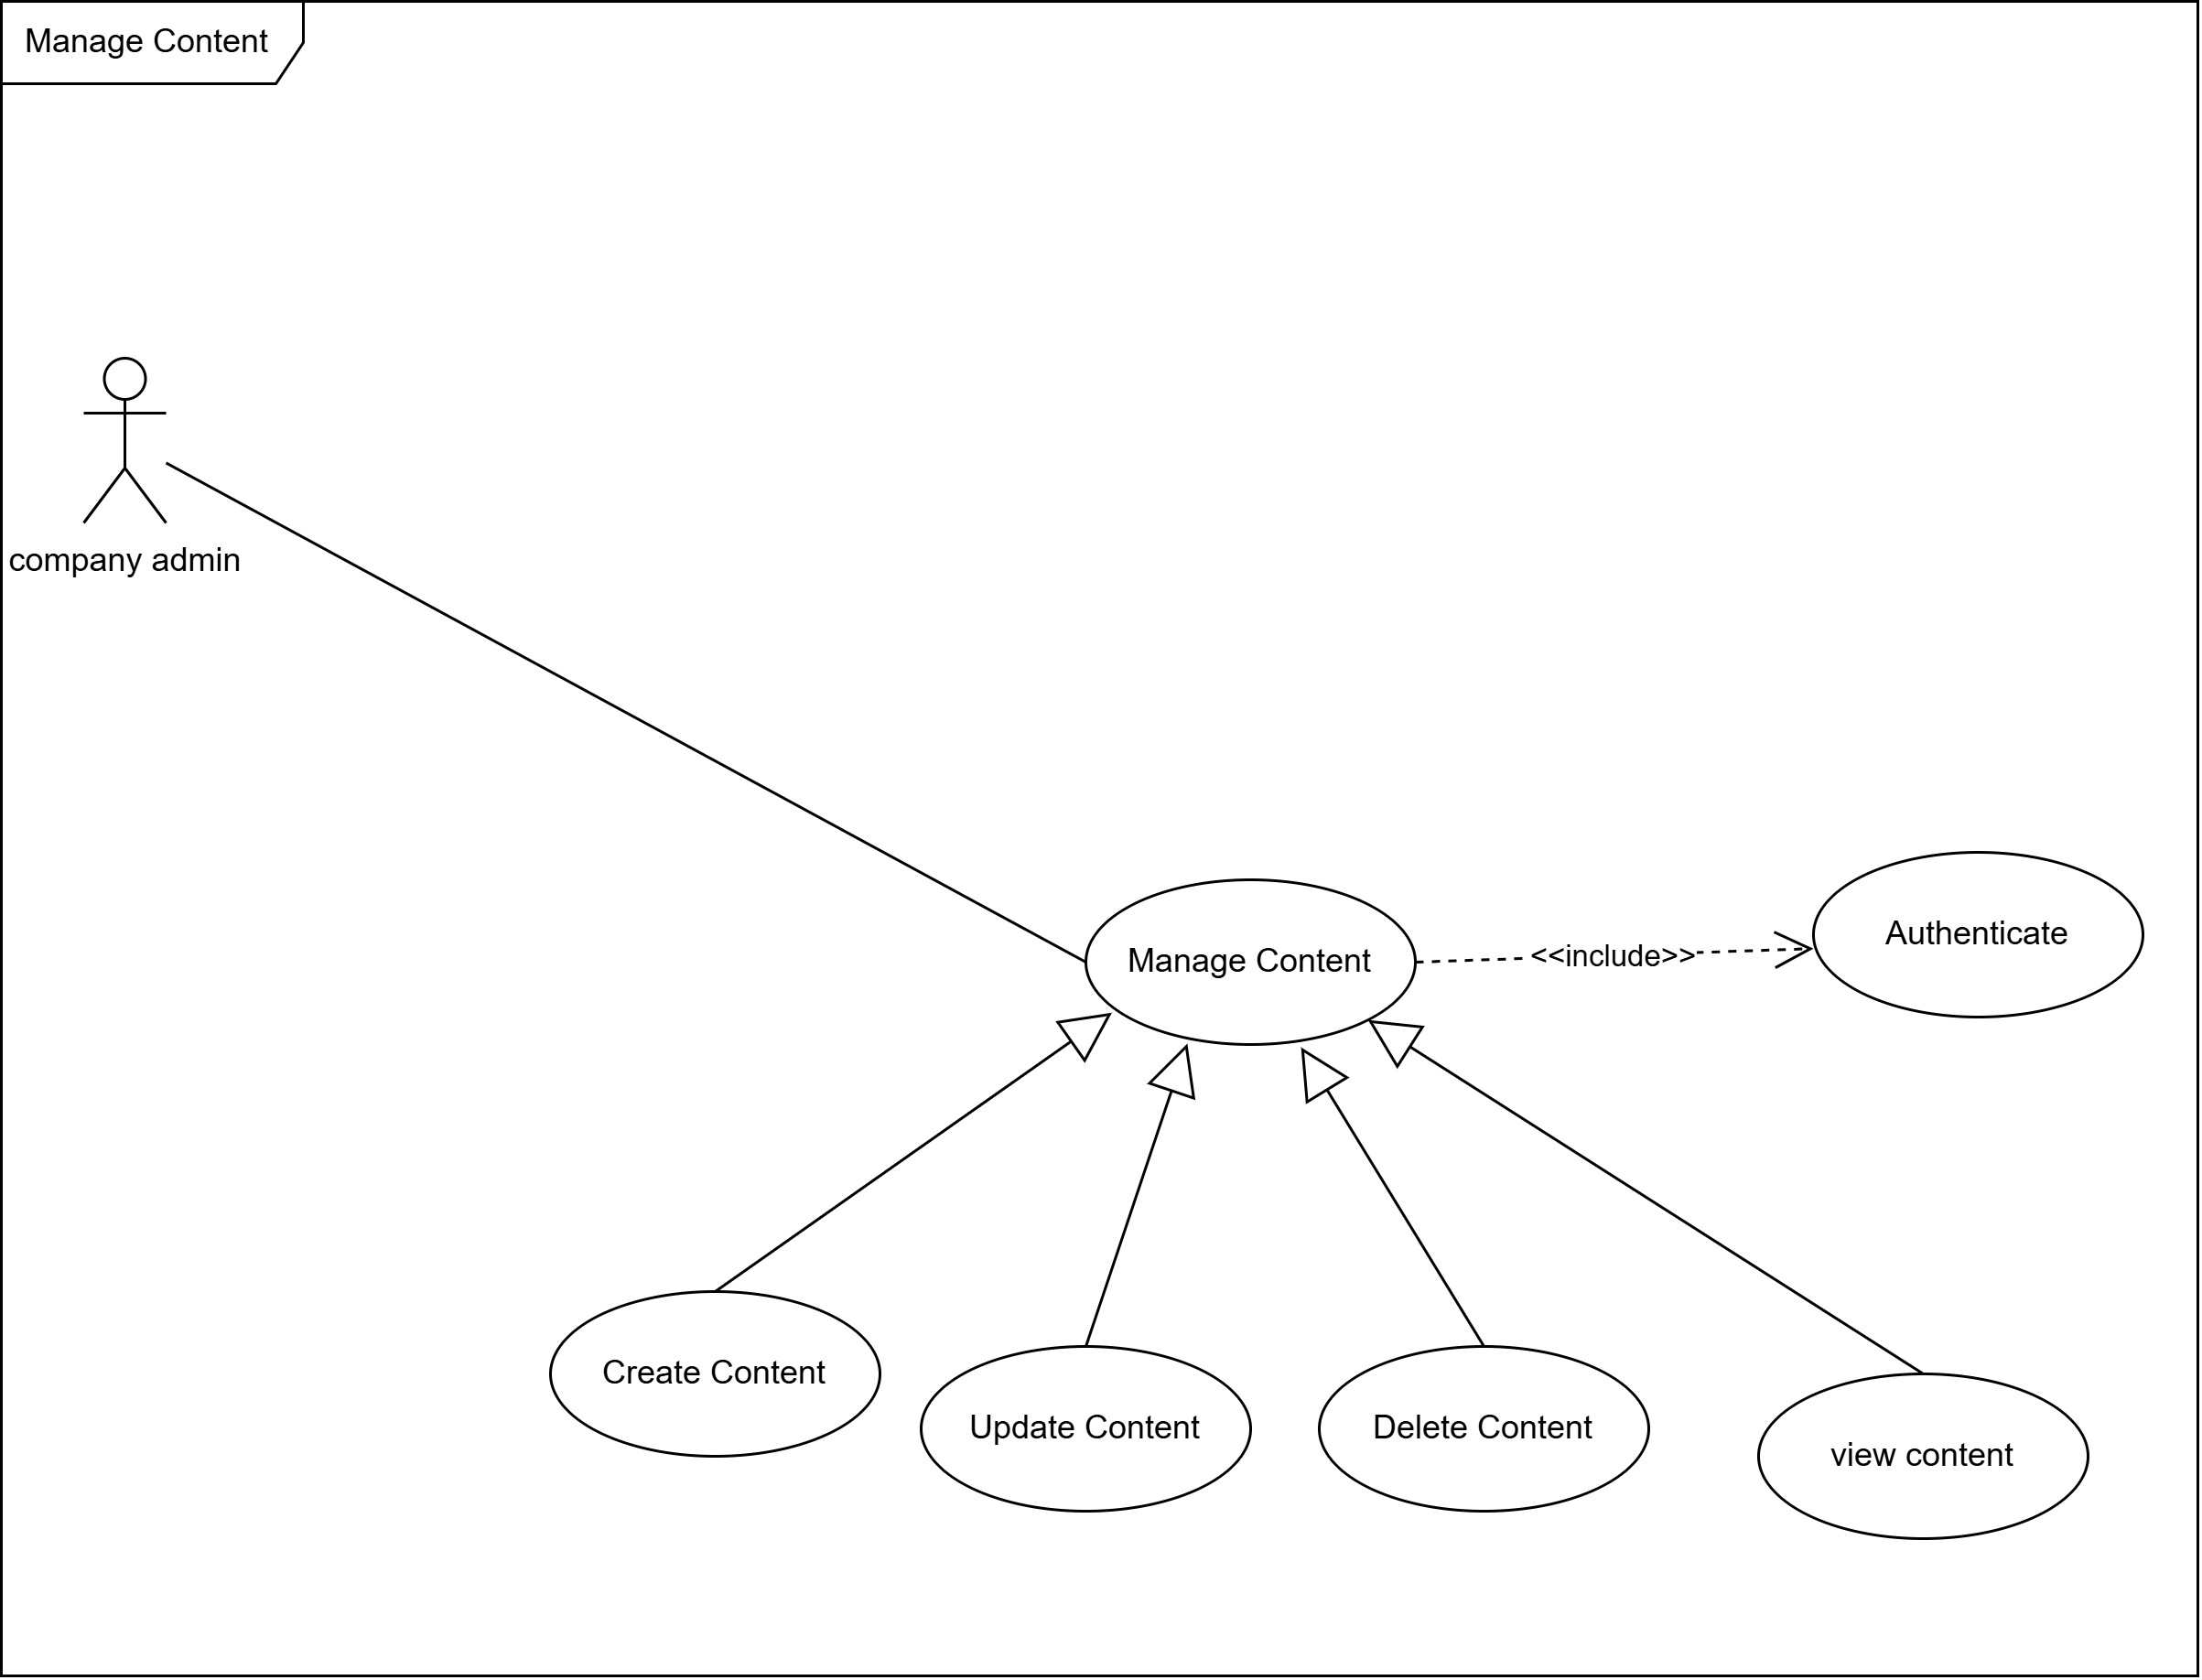
\includegraphics[width=0.8\textwidth]{images/usecase5.drawio.png}
\caption{Use case diagram: Manage Guides}
\label{fig:usecase_manage_guides}
\end{figure}

\begin{table}[!htbp]
\centering
\caption{Textual description of the Manage Guides use case}
\label{tab:manage_guides_desc}
\begin{tabular}{lp{10cm}}
\toprule
\textbf{Element} & \textbf{Description} \\
\midrule
Use Case & Manage Guides \\
Actor & Company Admin \\
Precondition & Authorized role (Technician or Brand Admin). \\
Postcondition & Markdown guide is published or saved as draft. \\
Nominal Scenario &
1. Writer picks a hardware product from list. \newline
2. App loads guide composer page. \newline
3. Writer drafts steps, embeds media files, and writes descriptions. \newline
4. Backend saves steps array in guide collection. \\
\bottomrule
\end{tabular}
\end{table}

\subsubsection{Use Case Refinement: Approve Content}

Our quality control pipeline relies on a formal review queue. Figure~\ref{fig:usecase_approve_content} and Table~\ref{tab:approve_content_desc} outline how we approve new submissions.

\begin{figure}[!htbp]
\centering
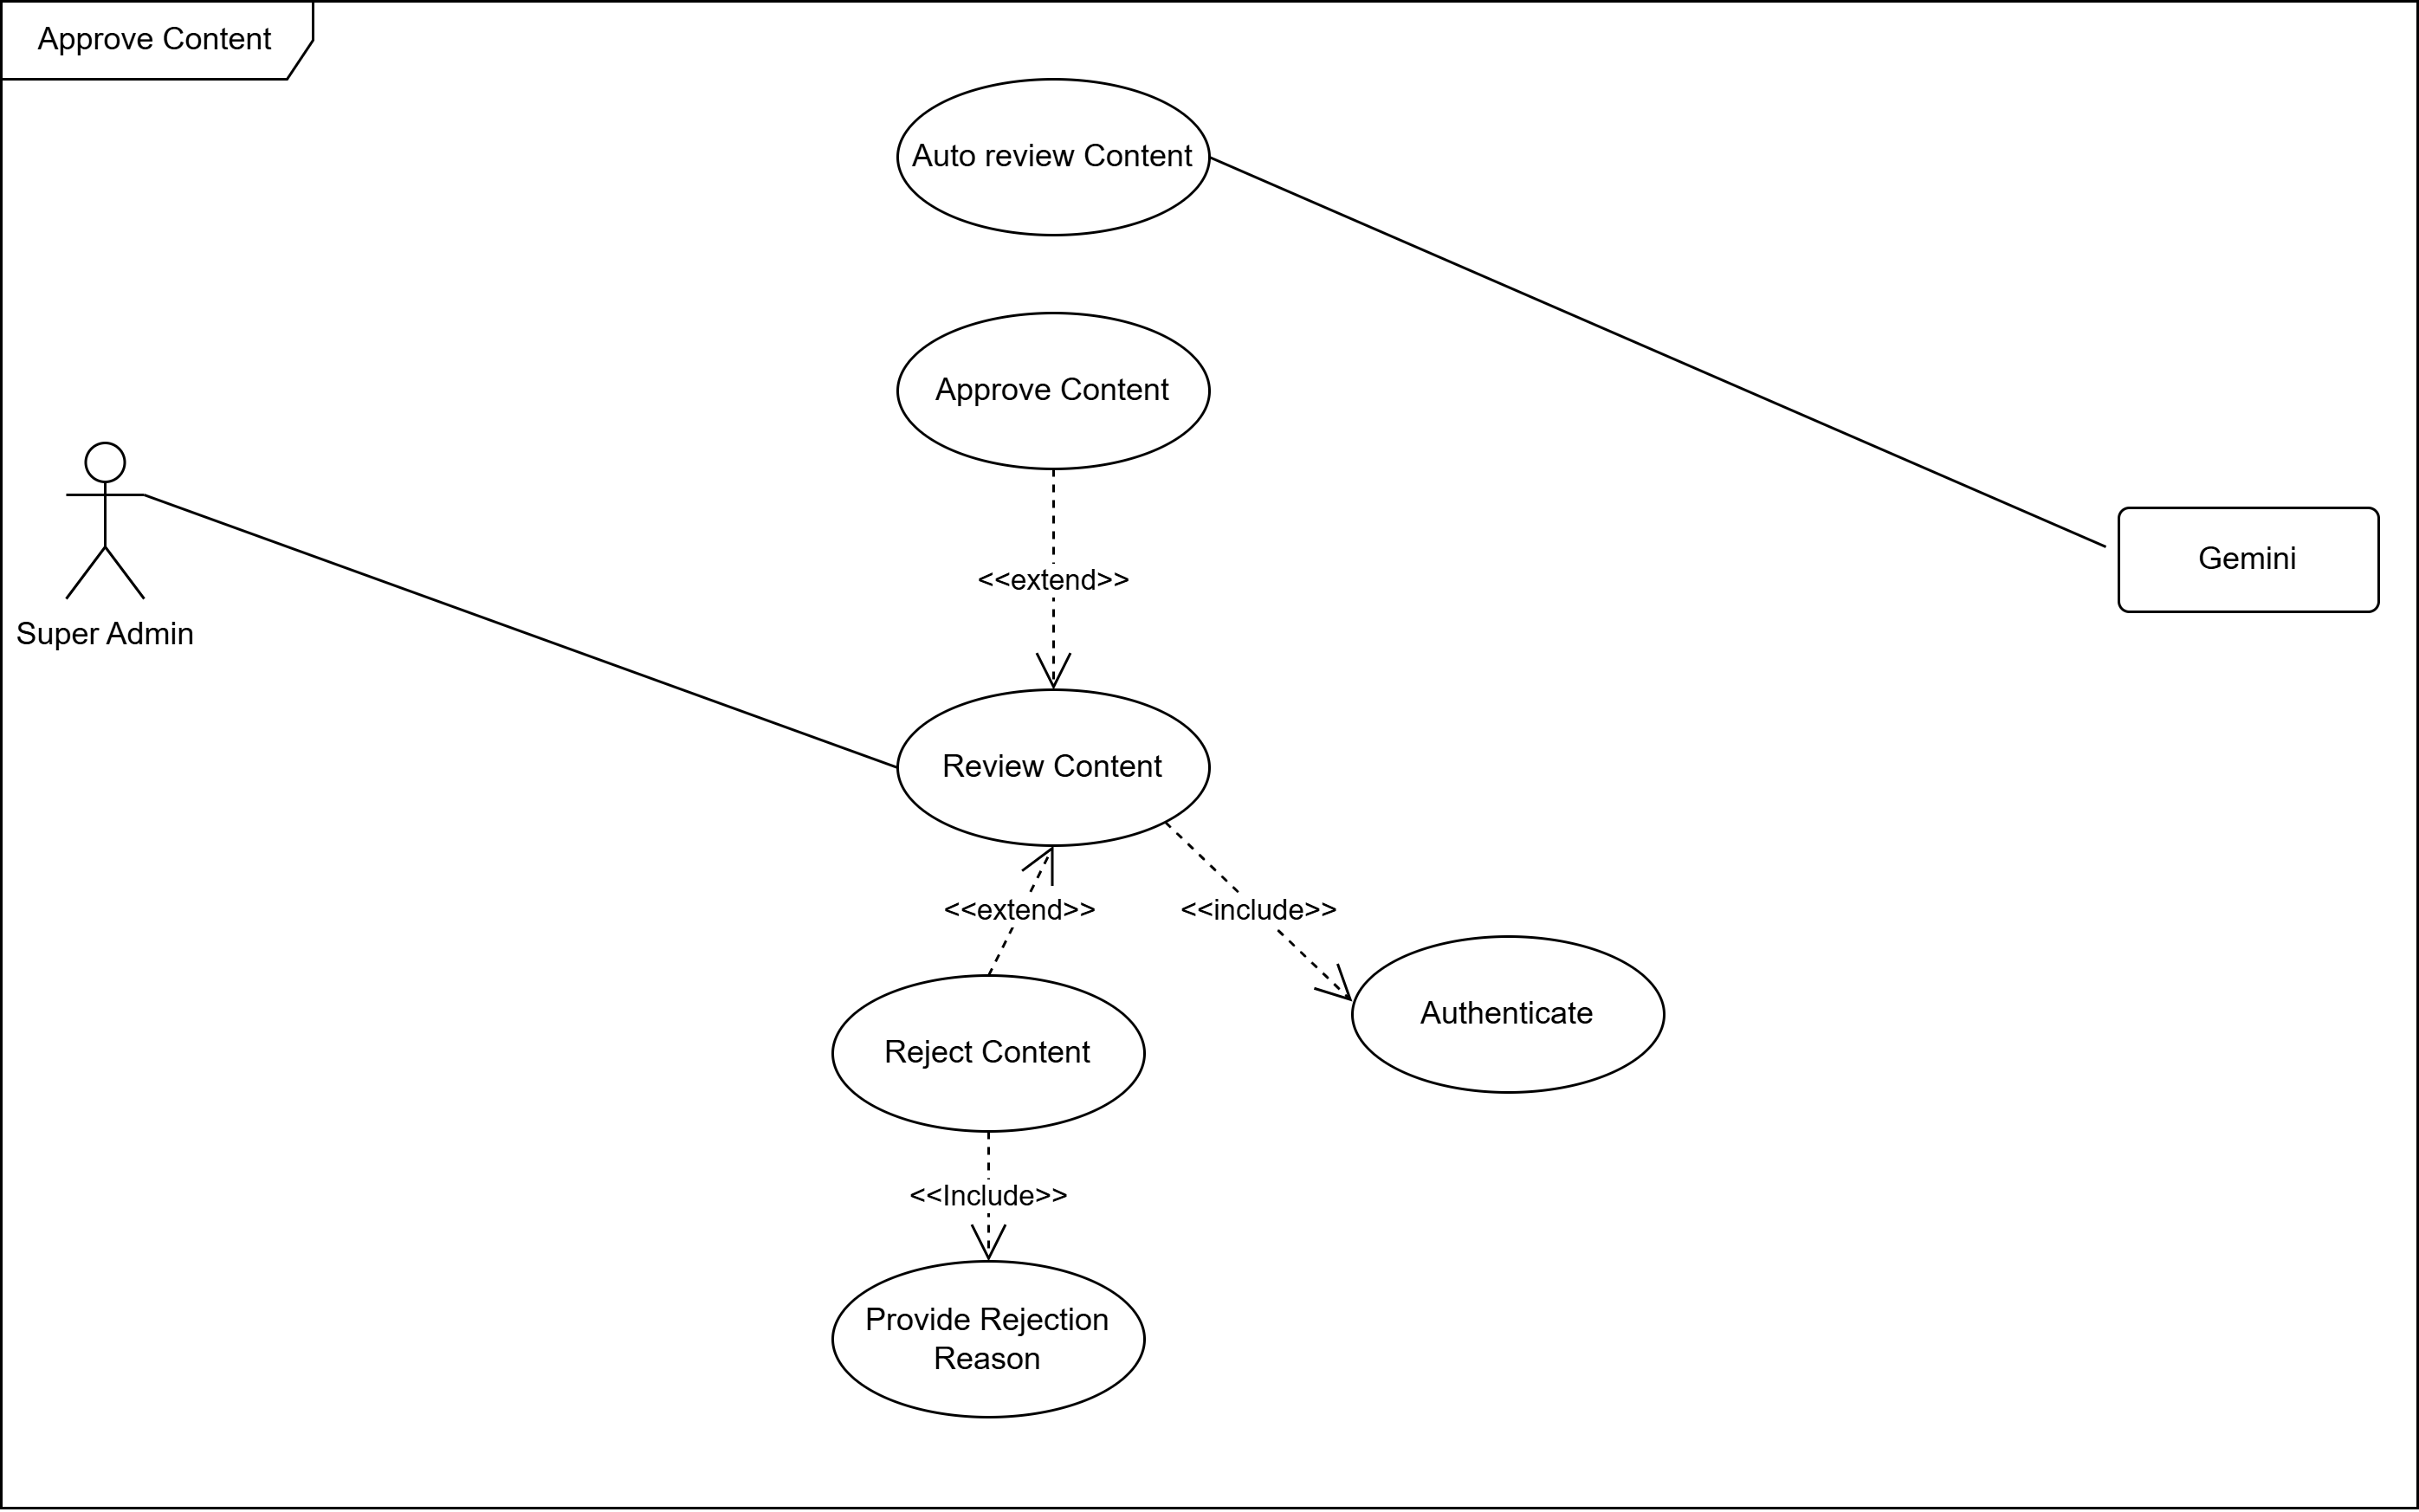
\includegraphics[width=0.8\textwidth]{images/usecase7.drawio.png}
\caption{Use case diagram: Approve Content}
\label{fig:usecase_approve_content}
\end{figure}

\begin{table}[!htbp]
\centering
\caption{Textual description of the Approve Content use case}
\label{tab:approve_content_desc}
\begin{tabular}{lp{10cm}}
\toprule
\textbf{Element} & \textbf{Description} \\
\midrule
Use Case & Approve Content \\
Actor & Company Admin / Super Admin \\
Precondition & A guide document is in 'pending' status. \\
Postcondition & Guide status is updated to 'published' or 'rejected'. \\
Nominal Scenario &
1. Technician submits guide draft for review. \newline
2. Backend sets guide status to pending and logs queue request. \newline
3. Brand manager opens queue and inspects steps. \newline
4. Manager clicks approve or reject, modifying document status. \\
\bottomrule
\end{tabular}
\end{table}

\subsection{Class Diagram}

Figure~\ref{fig:sprint2_class} shows the database schema for the catalog features. We structured the relationships so that each product belongs to a specific brand and category, keeping brand data isolated.

\begin{figure}[!htbp]
\centering
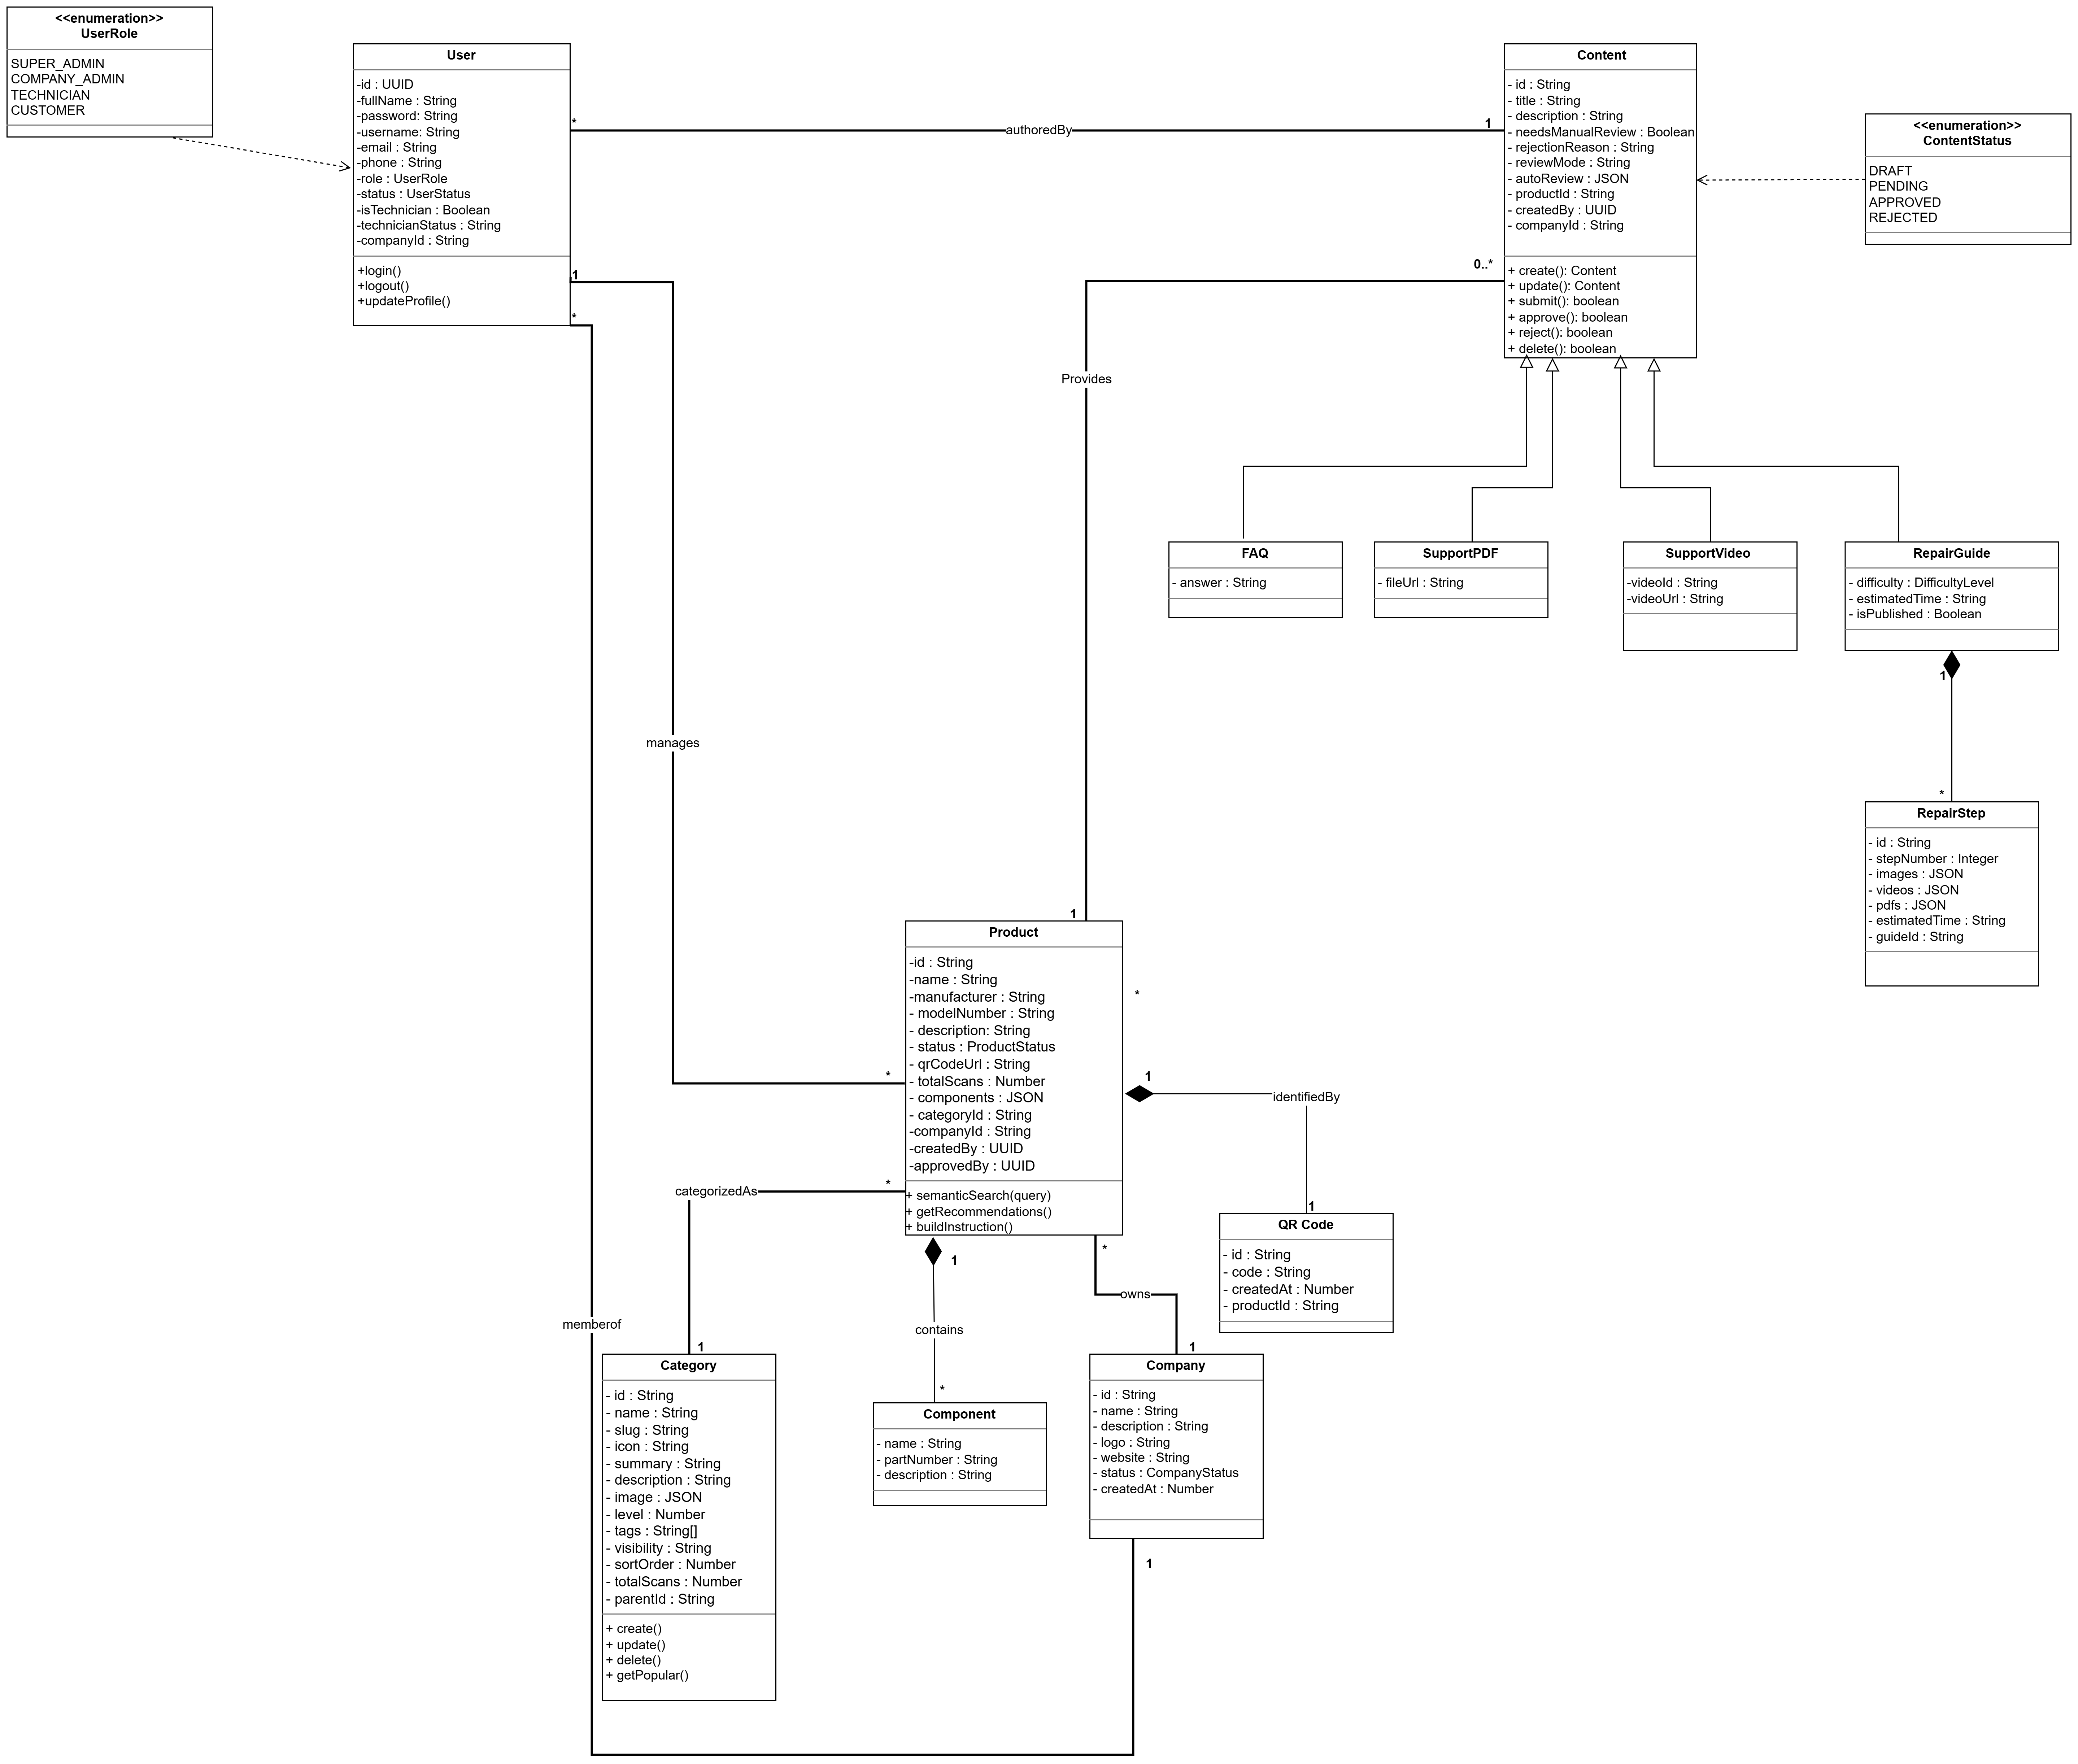
\includegraphics[width=0.9\textwidth]{images/sprint2class2.drawio.png}
\caption{Class diagram – Product, guide, and content approval}
\label{fig:sprint2_class}
\end{figure}

We defined these core relationships:
\begin{itemize}
    \item \textbf{Product}: The central hardware model. A product has multiple technical resources.
    \item \textbf{Guide}: Step-by-step instructions. A product can link to multiple guides.
    \item \textbf{Step}: The individual tasks within a guide. A guide contains an ordered list of steps.
    \item \textbf{Media}: Photos or videos linked to a step to clarify the instructions.
    \item \textbf{Content}: Contributed items (like FAQs or articles) that pass through our automatic AI check.
\end{itemize}

\subsection{Sequence Diagrams}

\subsubsection{Sequence Diagram: Product Management Flow}

Figure~\ref{fig:seq_product} details the message sequence when adding or updating product data.

\begin{figure}[!htbp]
\centering
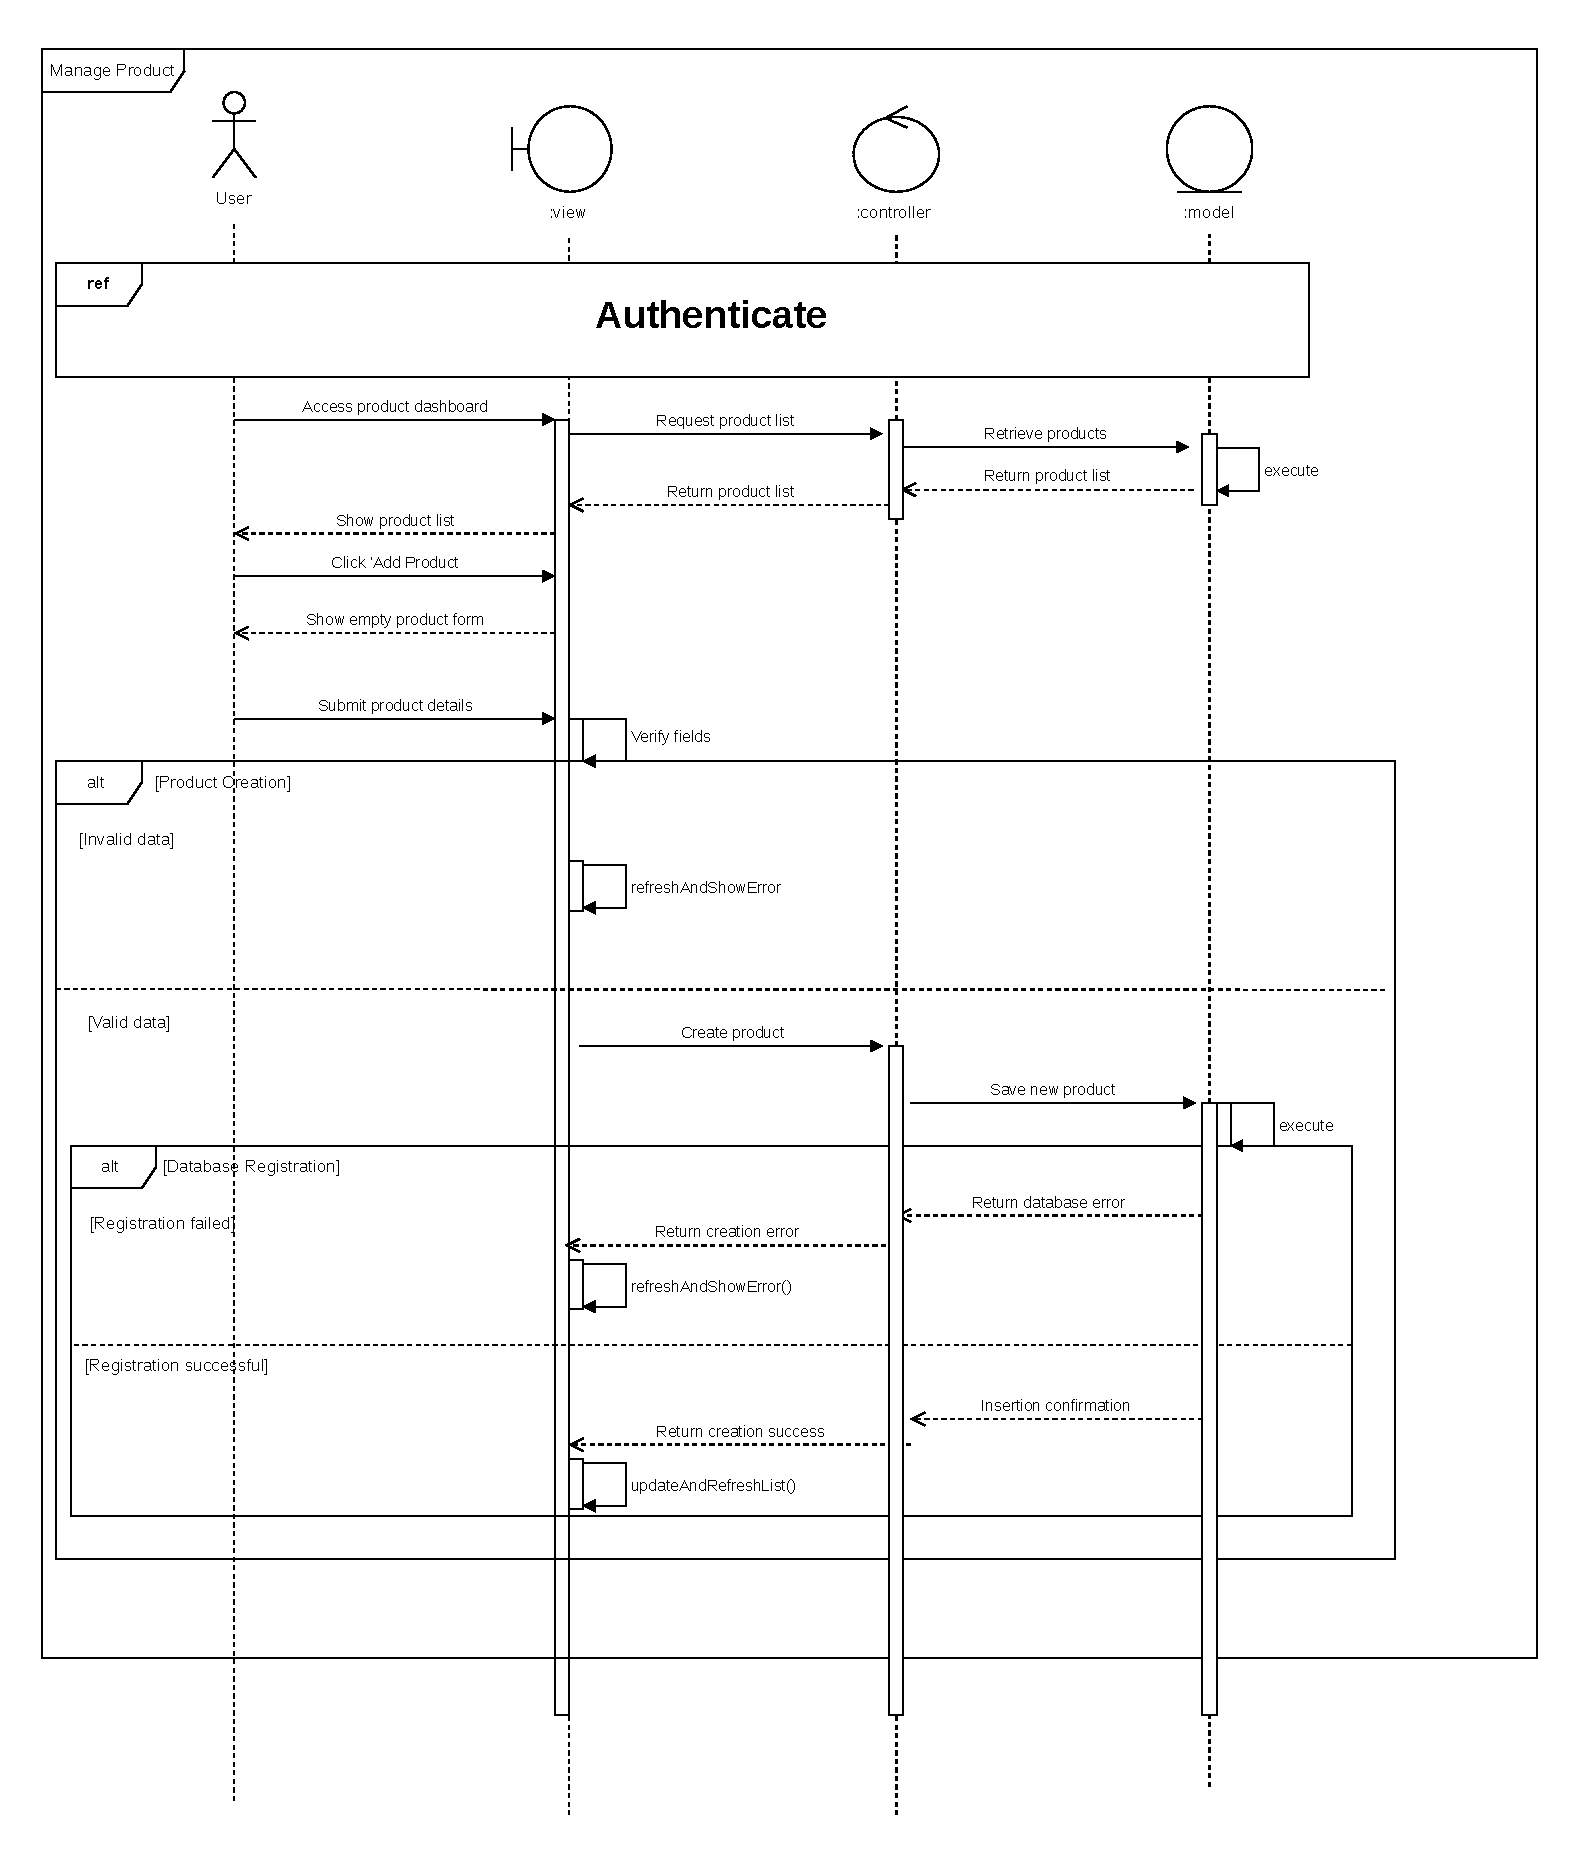
\includegraphics[width=0.9\textwidth]{images/seq3_product.pdf}
\caption{Sequence diagram: Product management}
\label{fig:seq_product}
\end{figure}

\subsubsection{Sequence Diagram: Content Creation \& Submission Flow}

Figure~\ref{fig:seq_content_submission} maps how the app handles draft content submissions and sends them to the review queue.

\begin{figure}[!htbp]
\centering
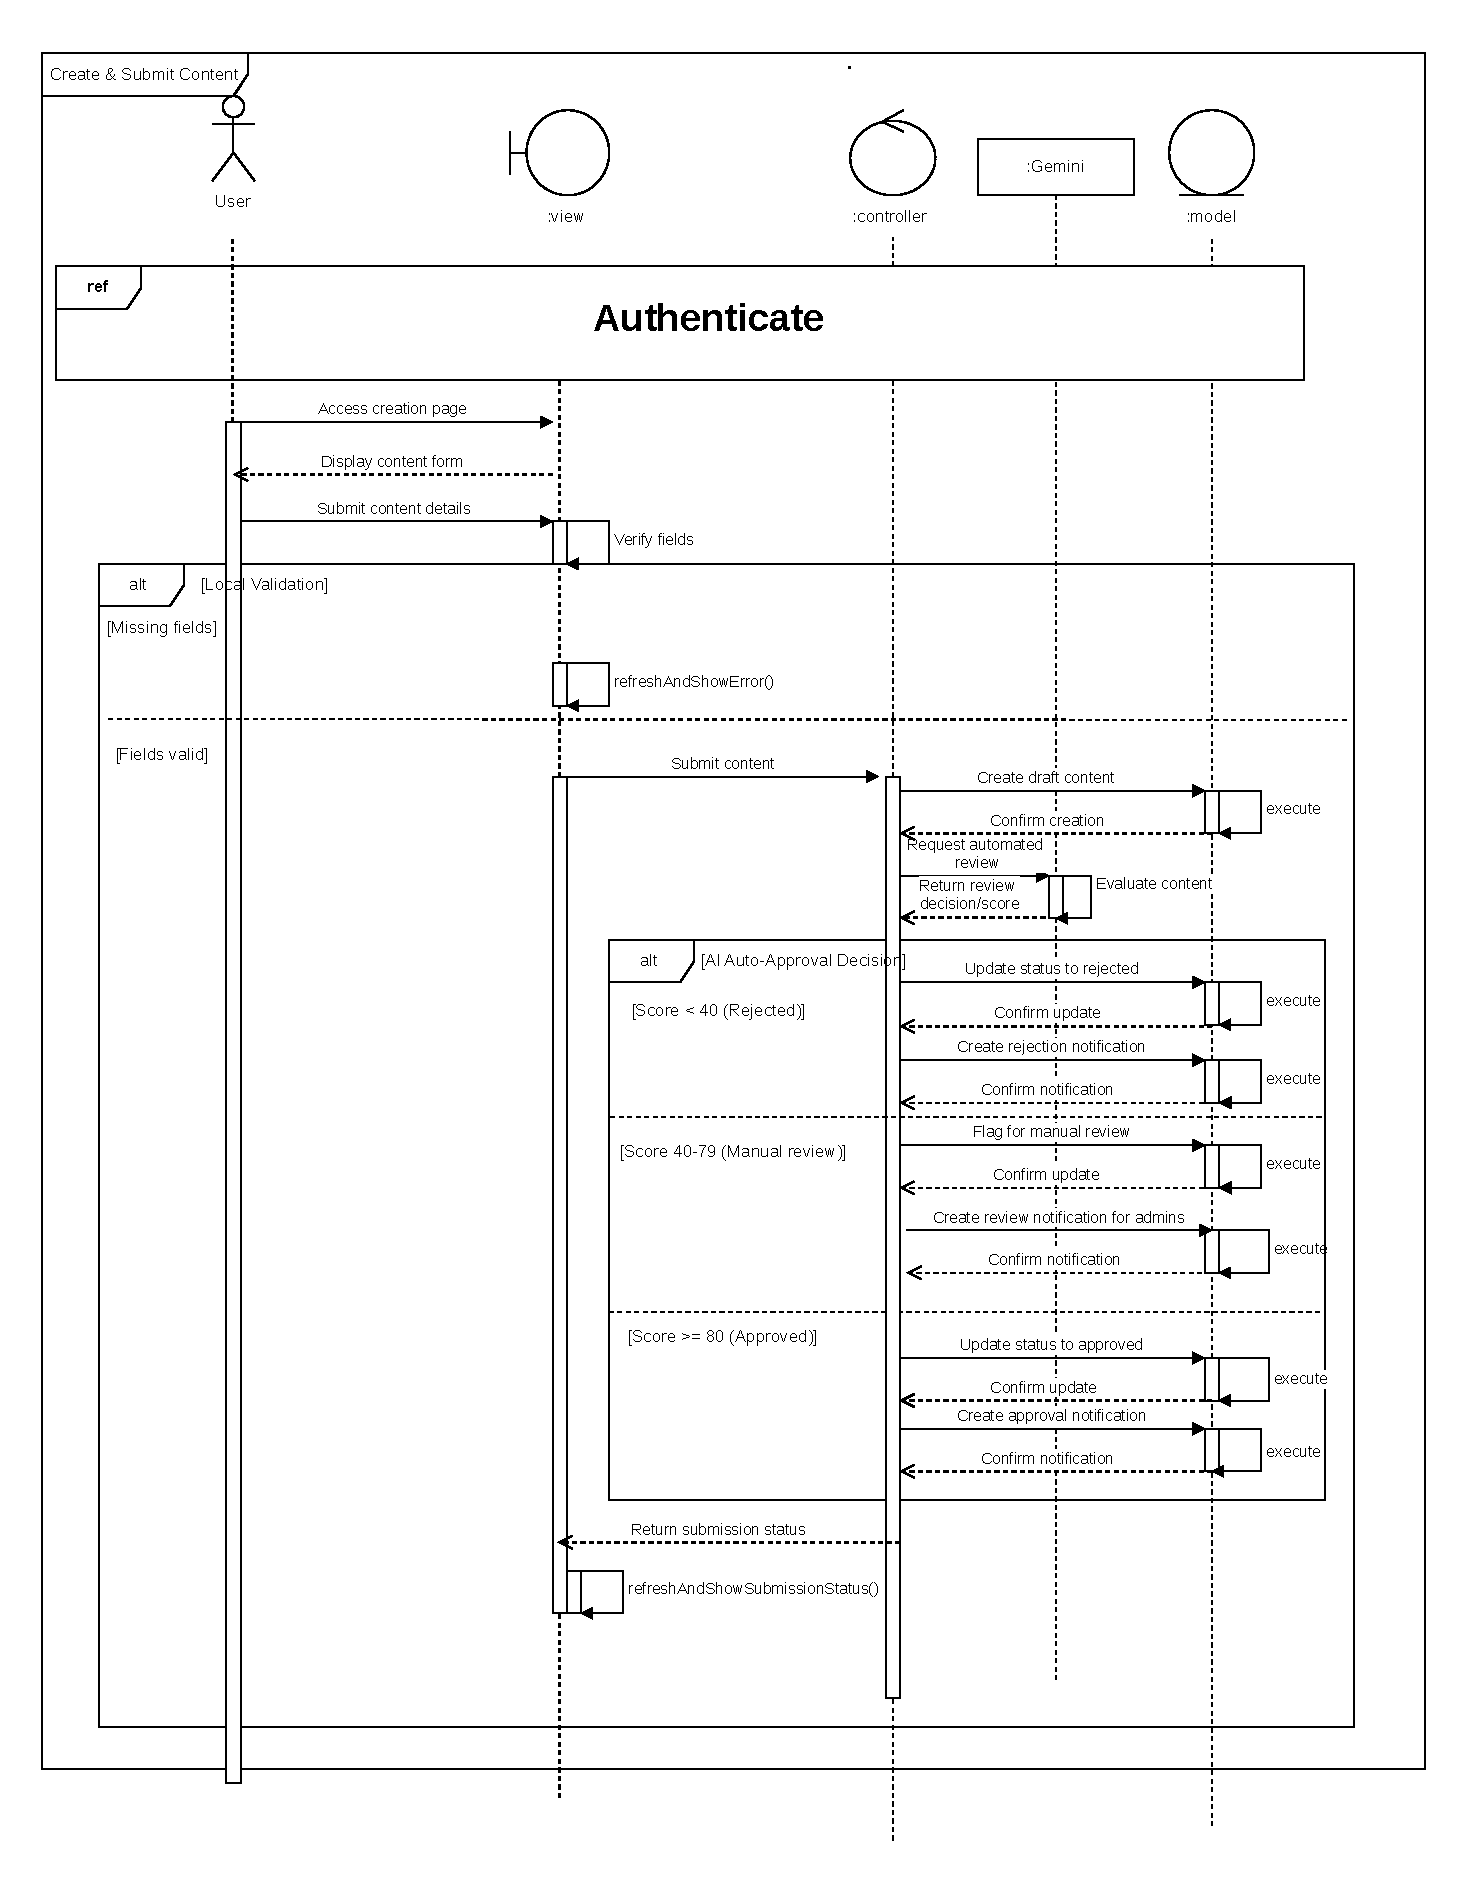
\includegraphics[width=0.95\textwidth]{images/seq4_content.pdf}
\caption{Sequence diagram: Content creation and submission}
\label{fig:seq_content_submission}
\end{figure}

\section{User Interface Overview}

\subsection{Web Interfaces}

We built the web administration dashboard to let companies organize products, write guides, and manage the moderation queue.

\begin{figure}[!htbp]
 \centering
 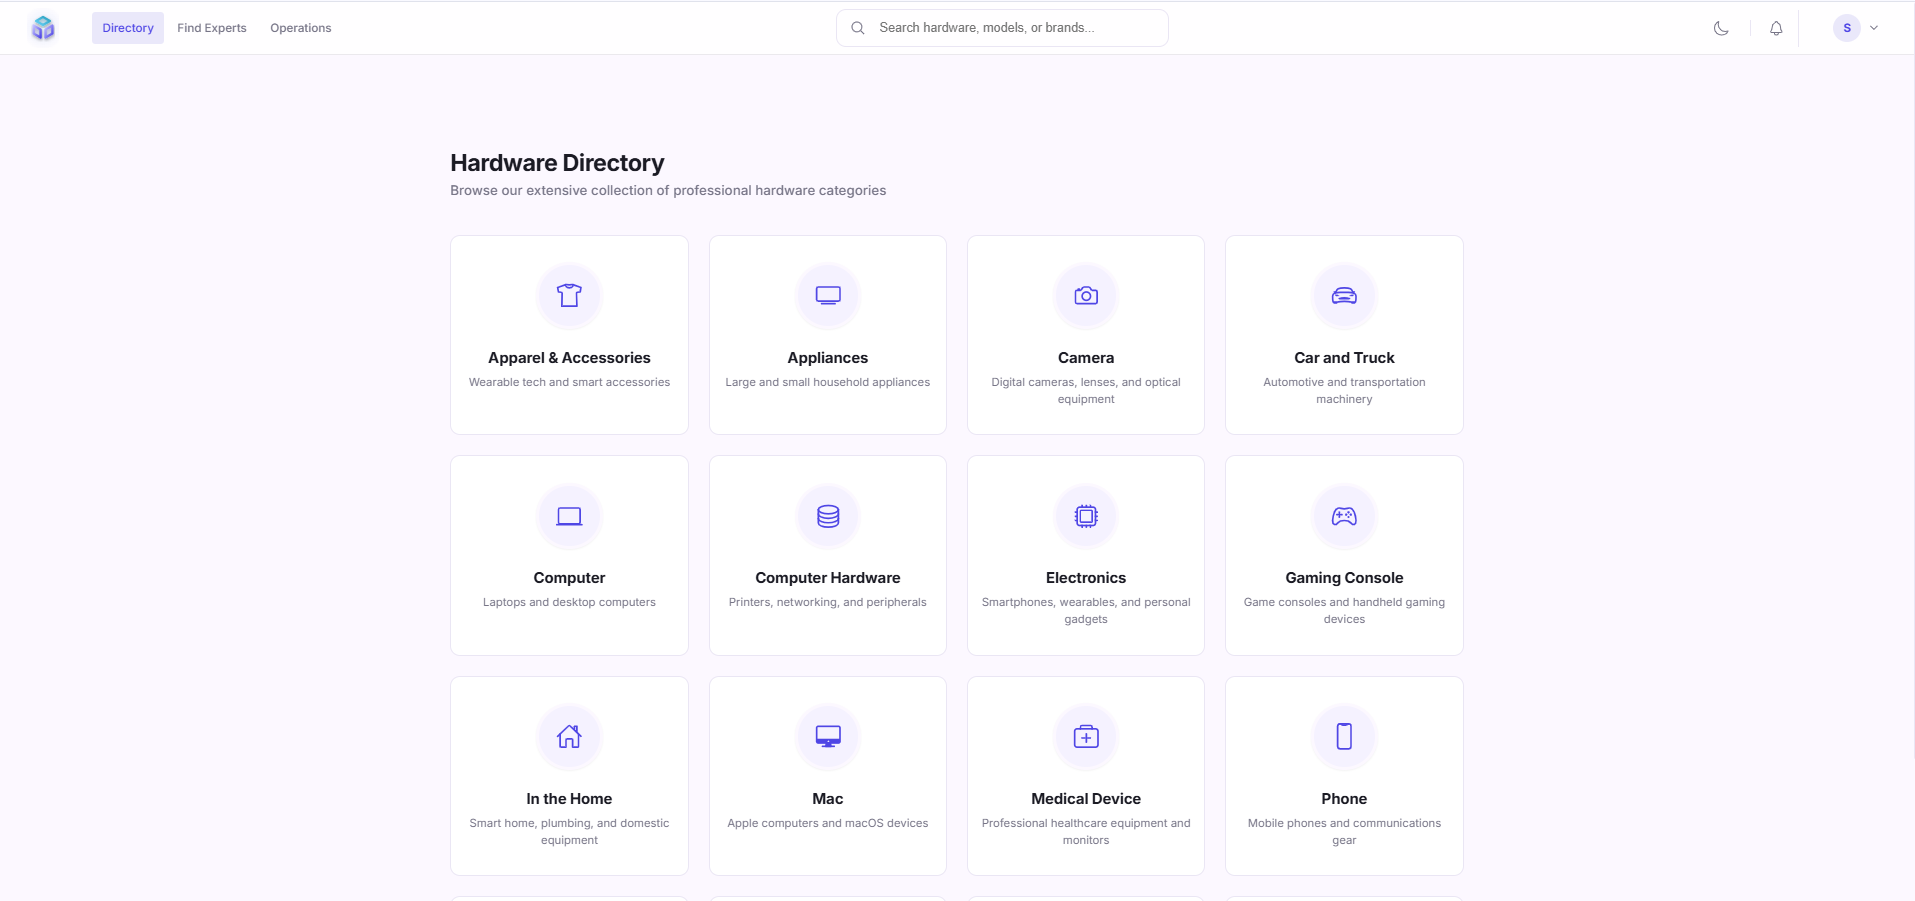
\includegraphics[width=0.45\textwidth]{images/product catalog.PNG}
 \hfill
 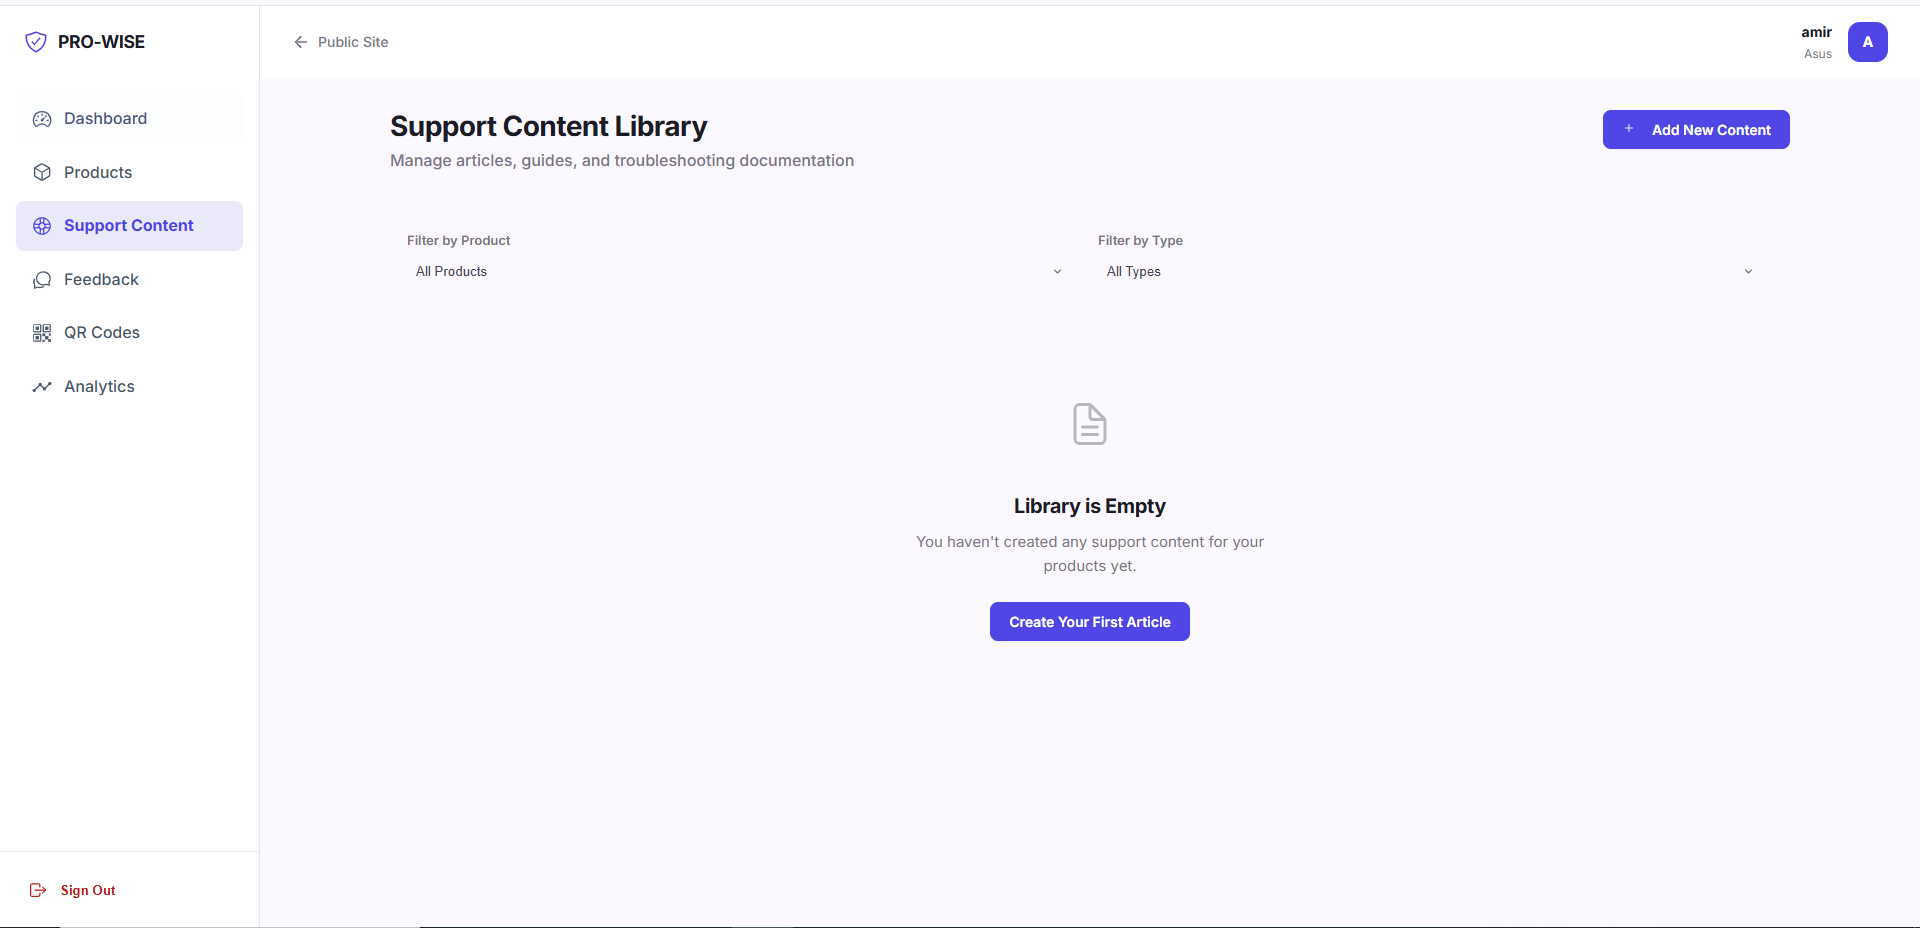
\includegraphics[width=0.45\textwidth]{images/content editor.PNG}
 \caption{Web interfaces – Product catalog and guide editor}
 \label{fig:web_catalog}
 \end{figure}
 
 \begin{figure}[!htbp]
 \centering
 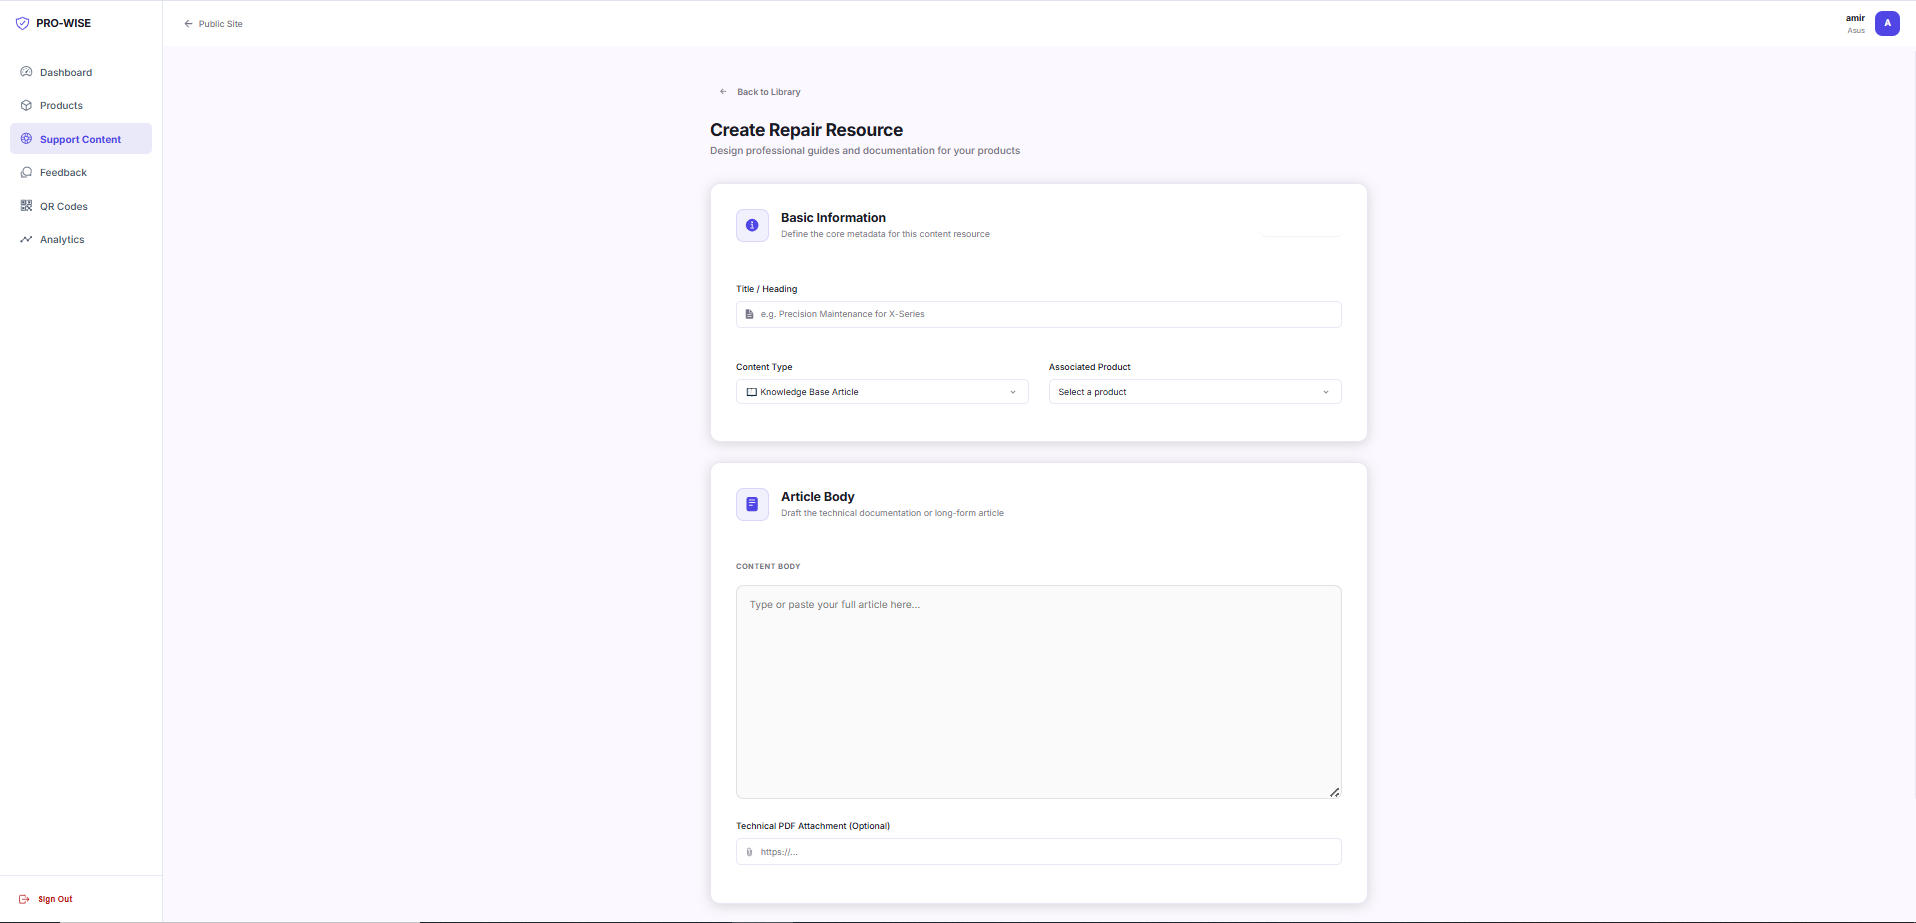
\includegraphics[width=0.45\textwidth]{images/content form.PNG}
 \hfill
 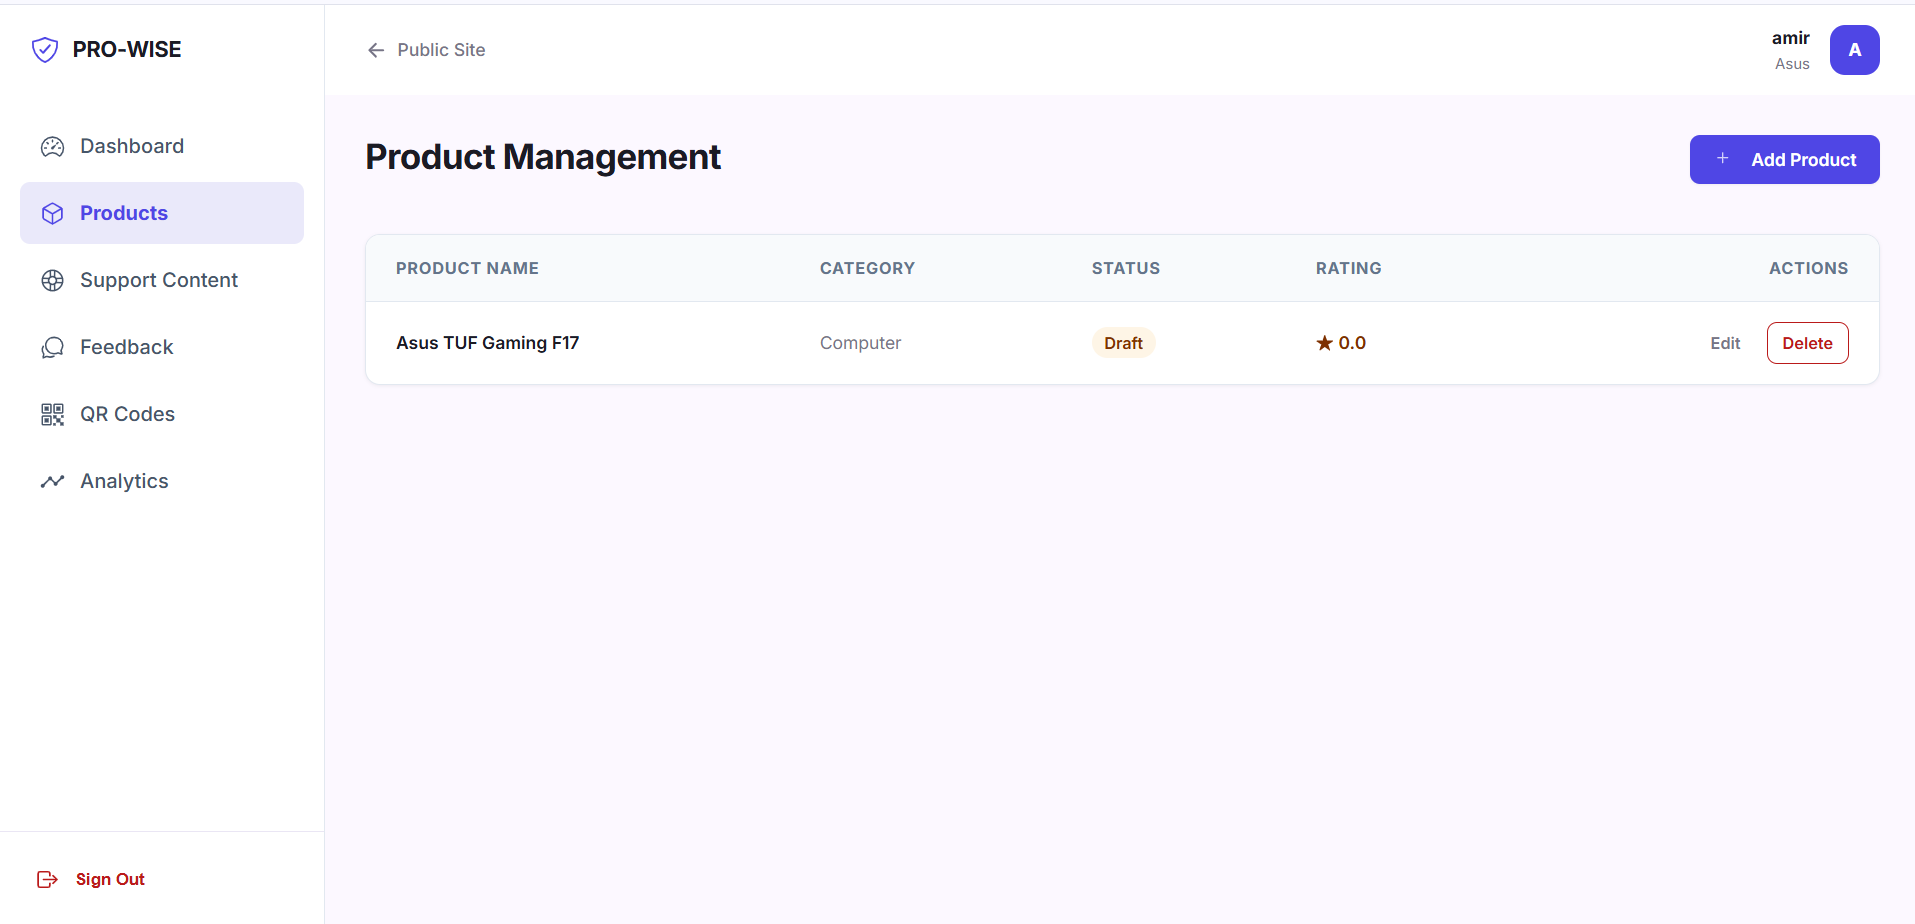
\includegraphics[width=0.45\textwidth]{images/product pending.PNG}
 \caption{Web interfaces – Content submission queue and moderation review dashboard}
 \label{fig:web_approval}
 \end{figure}

\subsection{Mobile Application Interfaces}

We drafted mobile sketches for the catalog. We prioritized the web portal to get the authoring engine running. Mobile guide consumption is detailed in Chapter 5.

\section{Conclusion}

We implemented the core catalog, guide editor, and moderation workflow. These components set the foundation for the upcoming feedback and analytics features.

\chapter{Release 3 : User Interactions, Feedback \& Platform Monitoring}

\section{Introduction}

This chapter details the development of real-time notification dispatchers, feedback submission forms, and background security logs. These additions transition our platform from a static guide viewer into an active portal.

We focused on developing four core features during Sprint 3:
\begin{itemize}
    \item \textbf{Feedback and Rating Engine}: We built rating forms and comments sections so that users can evaluate guides and products.
    \item \textbf{Real-Time Notifications}: We implemented an event dispatcher to alert users about state changes, such as document approvals or new technician assignments.
    \item \textbf{Security Auditing and Logging}: We wrote audit log utilities to record admin and company activity, helping to maintain security boundaries in our multi-tenant setup.
    \item \textbf{Usage Analytics Dashboard}: We aggregated product scan rates and feedback scores, displaying these trends on a dashboard for company admins.
\end{itemize}

\section{Sprint Backlog -- User Interactions and Monitoring}

Table~\ref{tab:sprint3_backlog} maps the backlog user stories chosen for Sprint 3, showing their priority levels and descriptions.

\renewcommand{\arraystretch}{1.3}
\setlength{\tabcolsep}{8pt}

\begin{table}[!htbp]
\centering
\caption{User stories for Release 3 (User Interactions and Monitoring)}
\label{tab:sprint3_backlog}
\resizebox{\textwidth}{!}{%
\begin{tabular}{clp{8cm}c}
\toprule
\textbf{ID} & \textbf{Feature / Epic} & \textbf{Description} & \textbf{Priority} \\
\midrule
12 & Feedback System & User ratings and comments on products and services & Medium \\
20 & Notification System & User notifications for updates and actions & Medium \\
19 & Activity Logs & Recording system actions for monitoring & Medium \\
18 & Analytics System & Tracking system usage and activity & Medium \\
\bottomrule
\end{tabular}%
}
\end{table}

\section{Refinement of Use Cases}

To design backend event listeners and database collections, we mapped out the main use cases for this sprint. These define preconditions and scenarios for review and audit trail features.

\subsection{Refinement of Sprint 3 Use Cases}

\subsubsection{Use Case Refinement: Submit Feedback}

Customers use the feedback form to rate products and comment on repair guides. Figure~\ref{fig:usecase_feedback} and Table~\ref{tab:feedback_desc} detail this interaction flow.

\begin{figure}[!htbp]
\centering
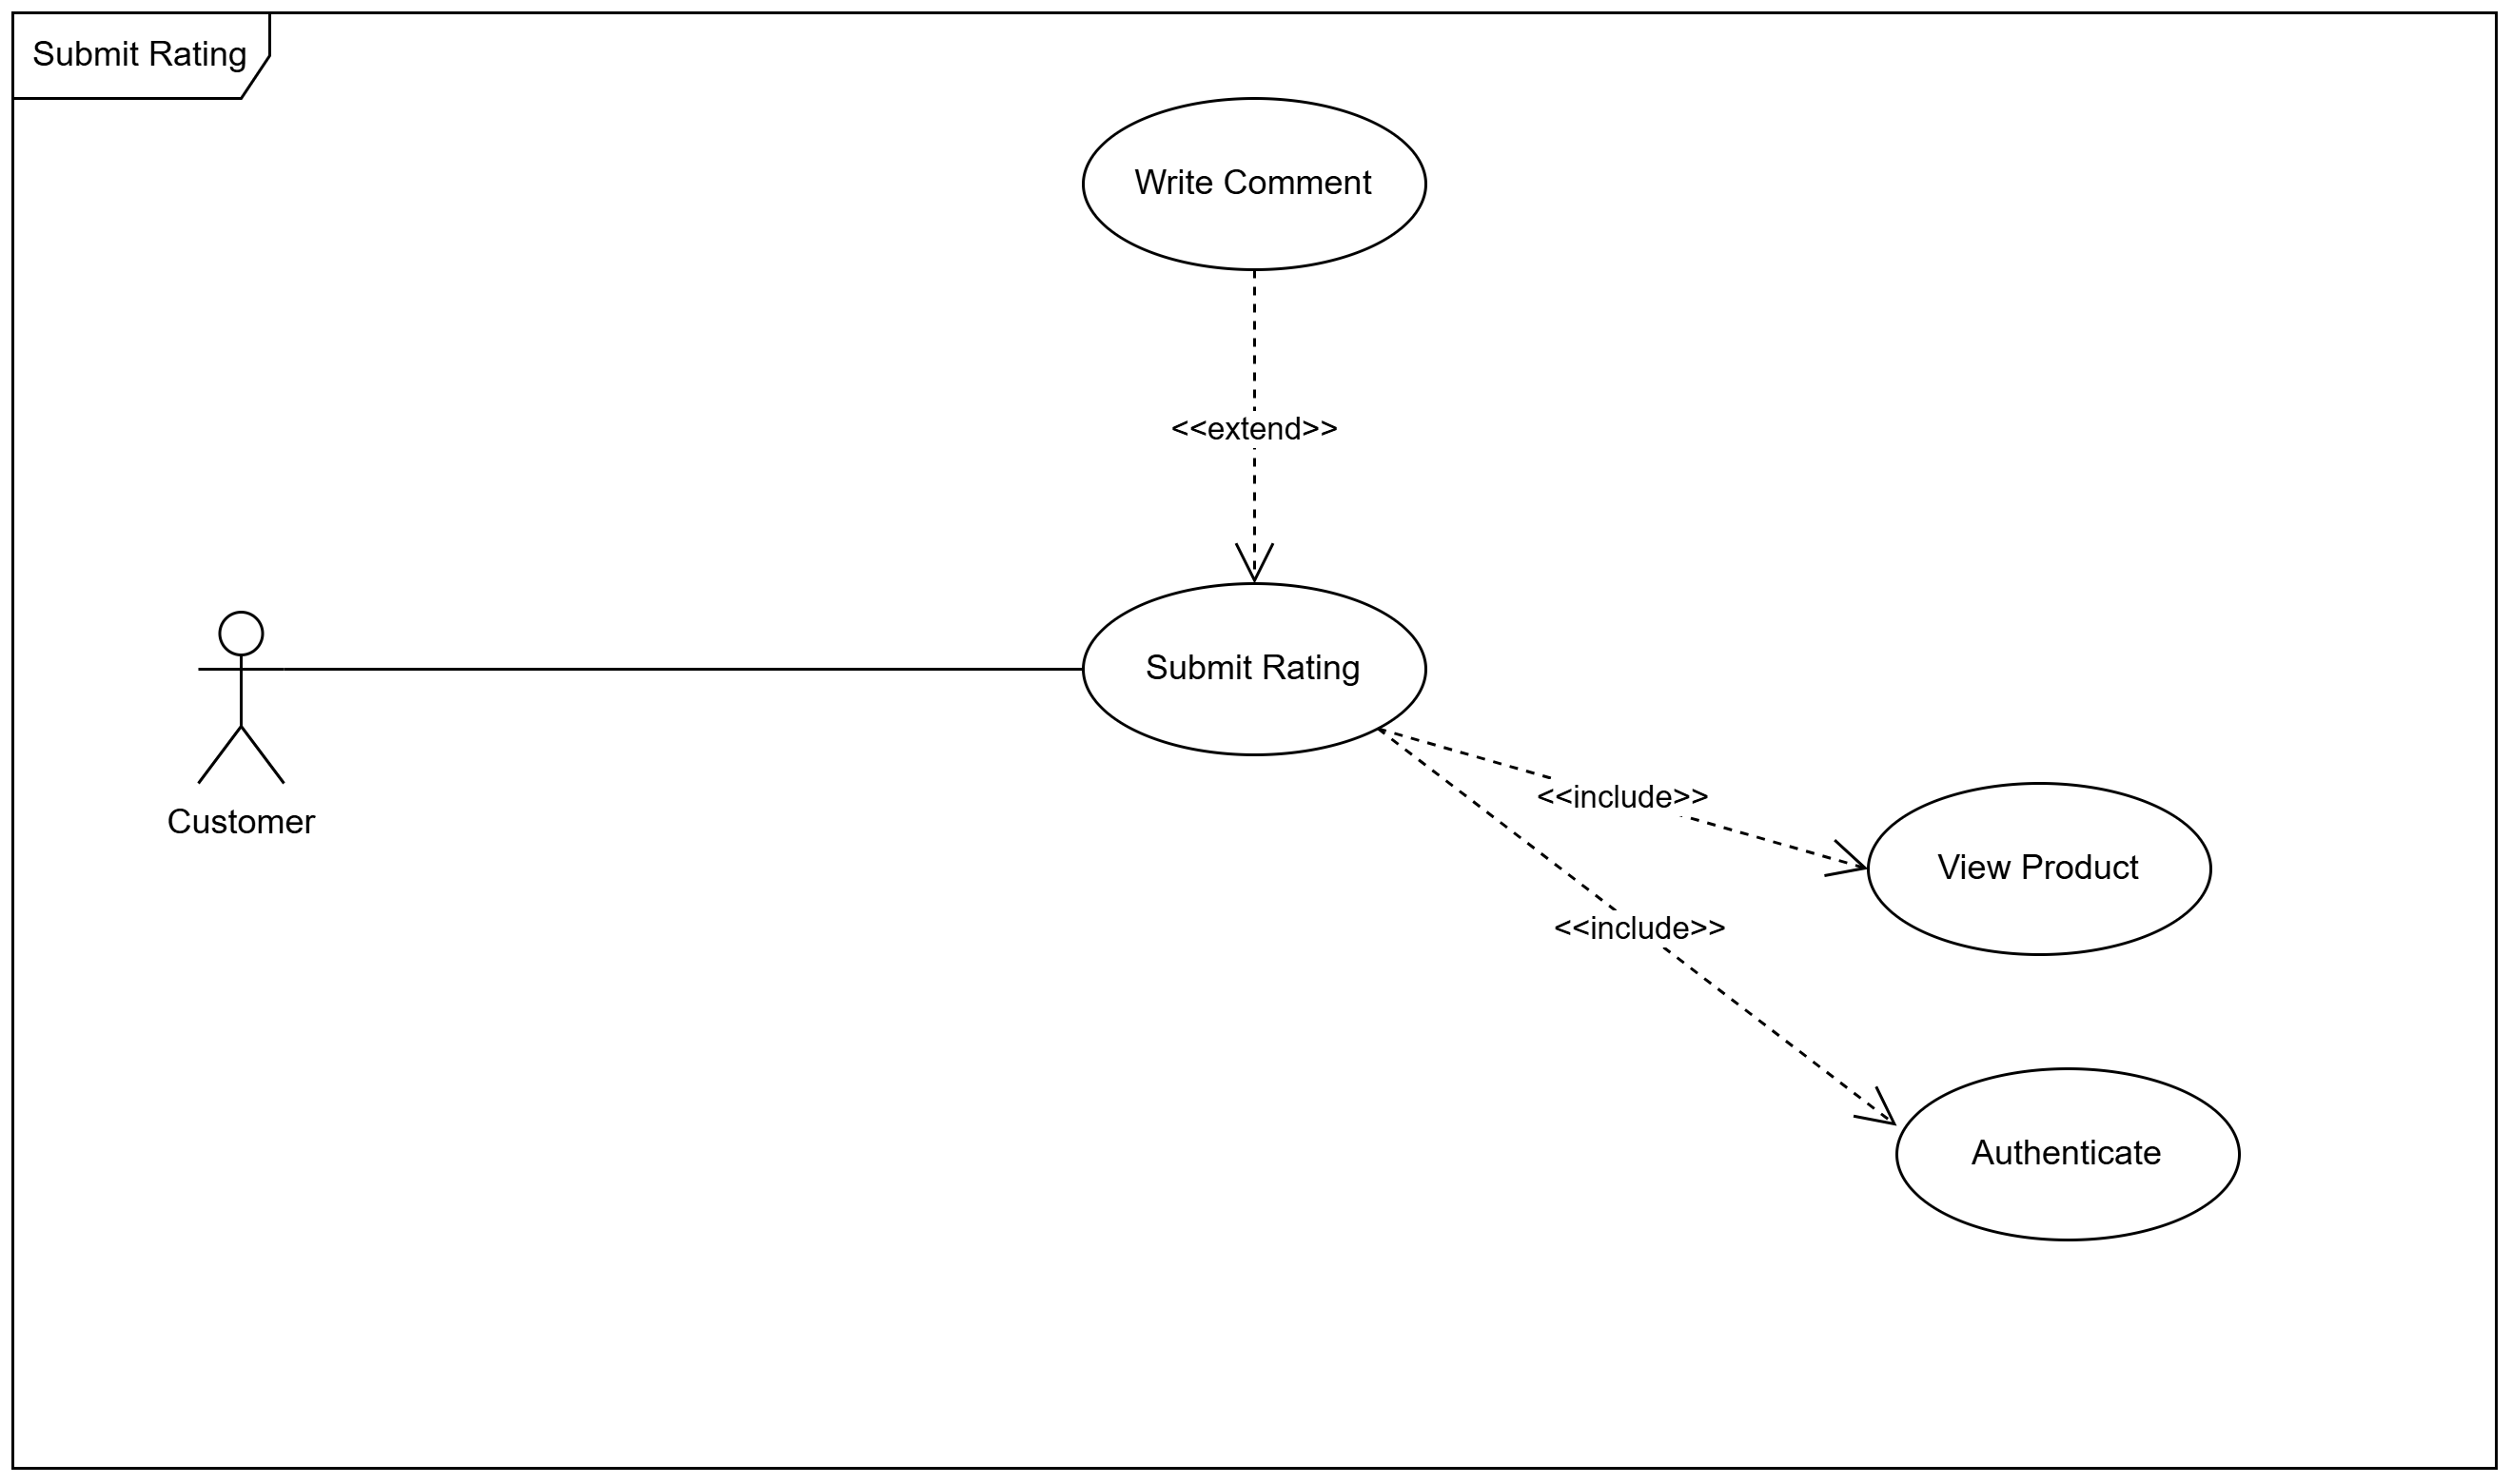
\includegraphics[width=0.8\textwidth]{images/usecase6.drawio.png}
\caption{Use case diagram: Submit Feedback}
\label{fig:usecase_feedback}
\end{figure}

\begin{table}[!htbp]
\centering
\caption{Textual description of the Submit Feedback use case}
\label{tab:feedback_desc}
\begin{tabular}{lp{10cm}}
\toprule
\textbf{Element} & \textbf{Description} \\
\midrule
Use Case & Submit Feedback \\
Actor & Client (Customer) \\
Precondition & Client has active session and opens model page. \\
Postcondition & Review is saved and model score recalculated. \\
Nominal Scenario &
1. Client opens a product page. \newline
2. Client types a comment and selects rating. \newline
3. Client submits rating form. \newline
4. Backend saves review and triggers average rating aggregation. \\
\bottomrule
\end{tabular}
\end{table}

\subsubsection{Use Case Refinement: View Notifications}

Our notification view lists alerts tailored to the logged-in user. Figure~\ref{fig:usecase_notifications} and Table~\ref{tab:notifications_desc} outline how we retrieve and mark these alerts as read.

\begin{figure}[!htbp]
\centering
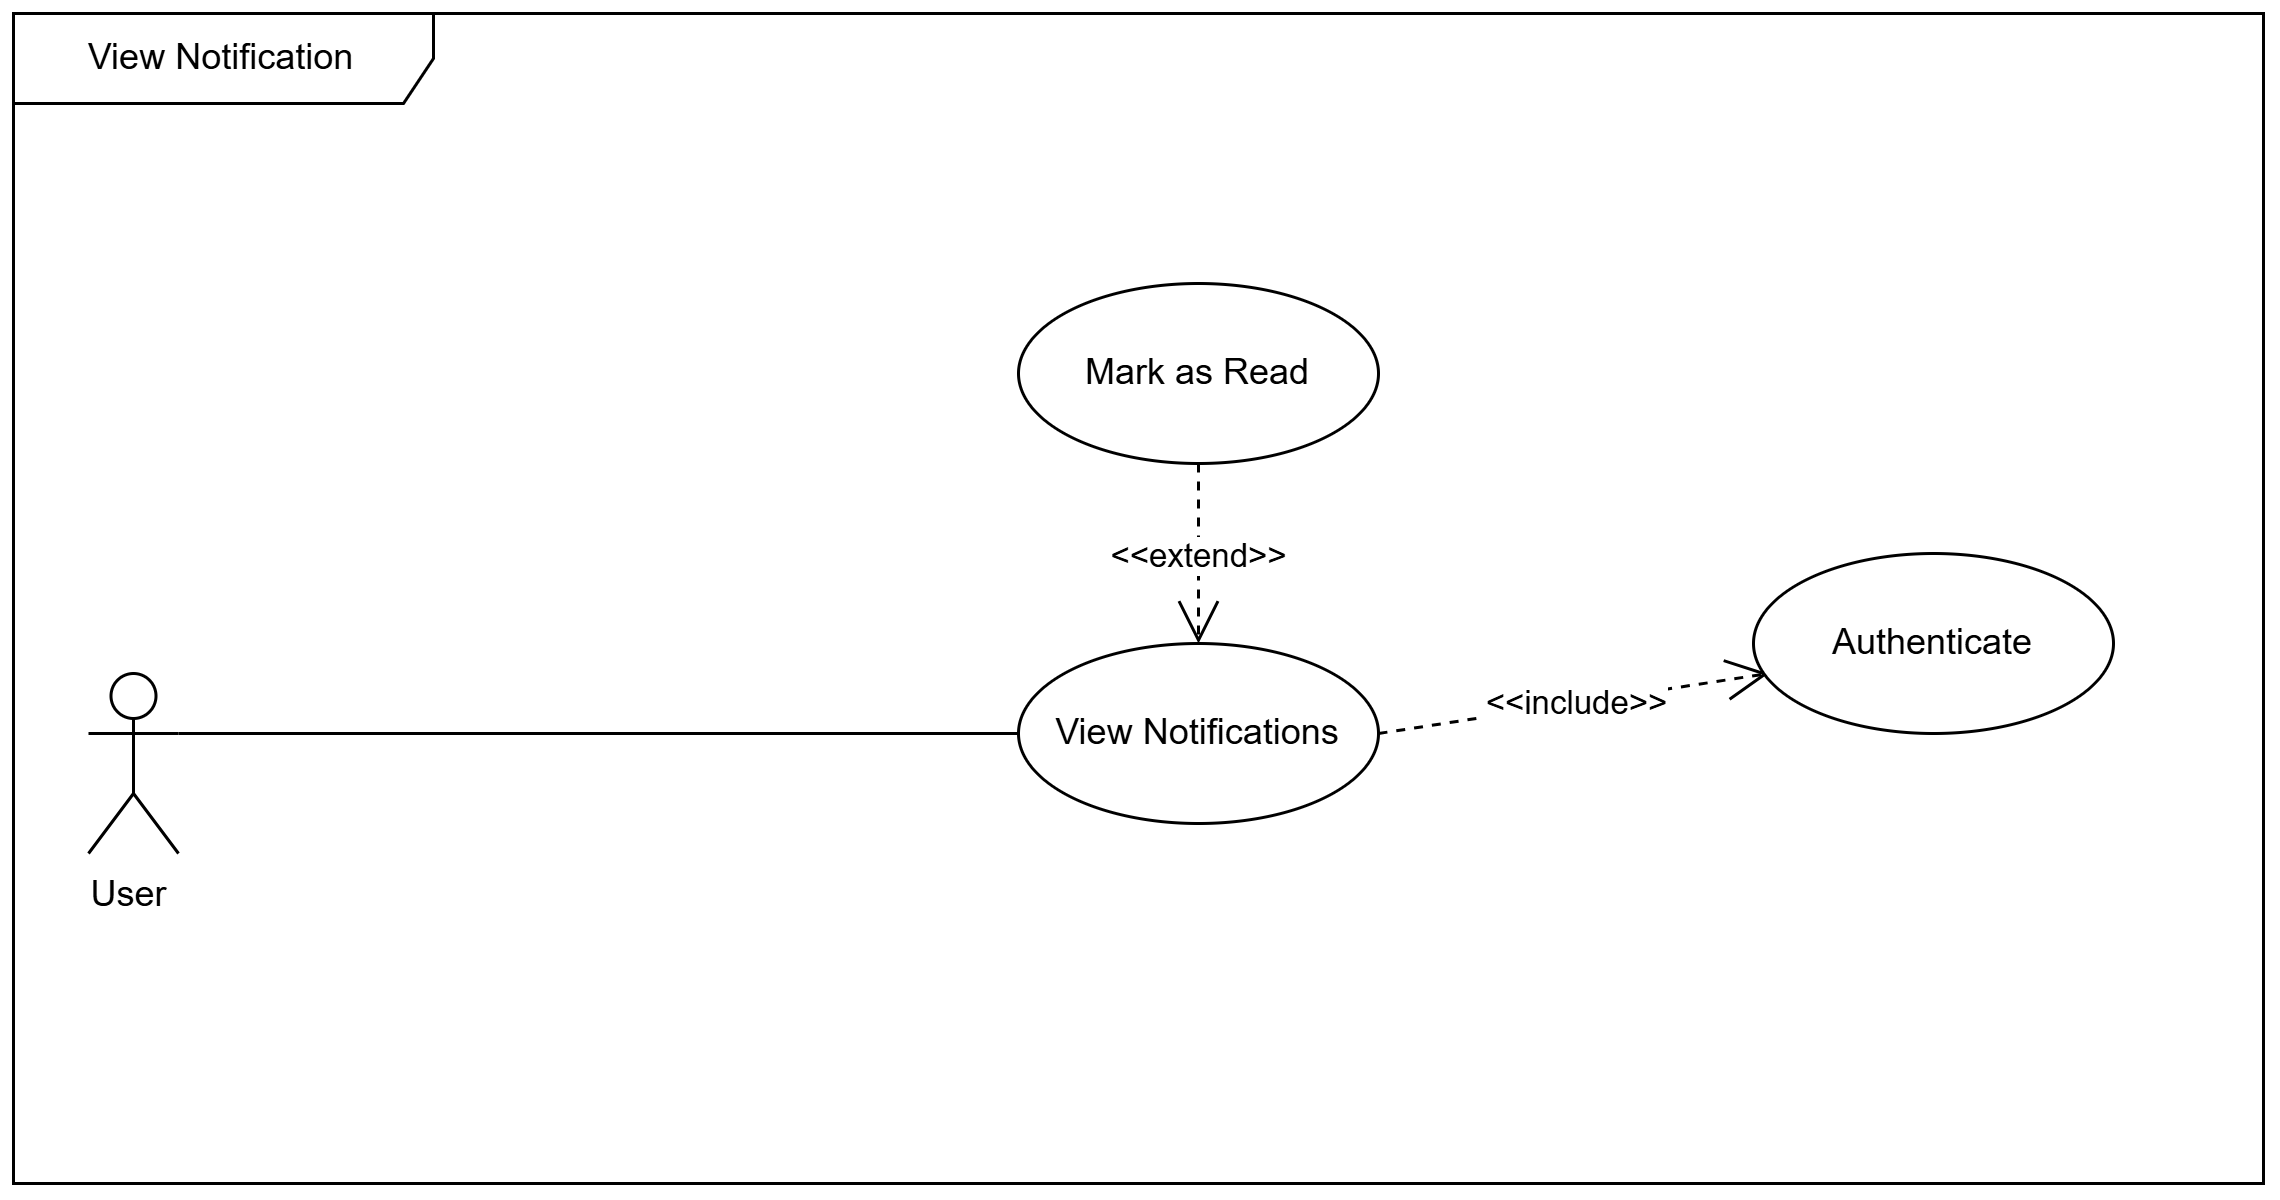
\includegraphics[width=0.8\textwidth]{images/usecase10.drawio.png}
\caption{Use case diagram: View Notifications}
\label{fig:usecase_notifications}
\end{figure}

\begin{table}[!htbp]
\centering
\caption{Textual description of the View Notifications use case}
\label{tab:notifications_desc}
\begin{tabular}{lp{10cm}}
\toprule
\textbf{Element} & \textbf{Description} \\
\midrule
Use Case & View Notifications \\
Actor & Client / Technician / Admin \\
Precondition & Active JWT cookie is present. \\
Postcondition & Notification documents are updated in the database. \\
Nominal Scenario &
1. User logs in and sees unread alert badge. \newline
2. User clicks notification center. \newline
3. Client opens recent alerts list. \newline
4. API sets alert status to 'read' in background. \\
\bottomrule
\end{tabular}
\end{table}

\subsubsection{Use Case Refinement: Track Activity Logs}

The audit system automatically records admin modifications in the database. Figure~\ref{fig:usecase_activity} and Table~\ref{tab:activity_desc} show how the log service aggregates metadata when changes occur.

\begin{figure}[!htbp]
\centering
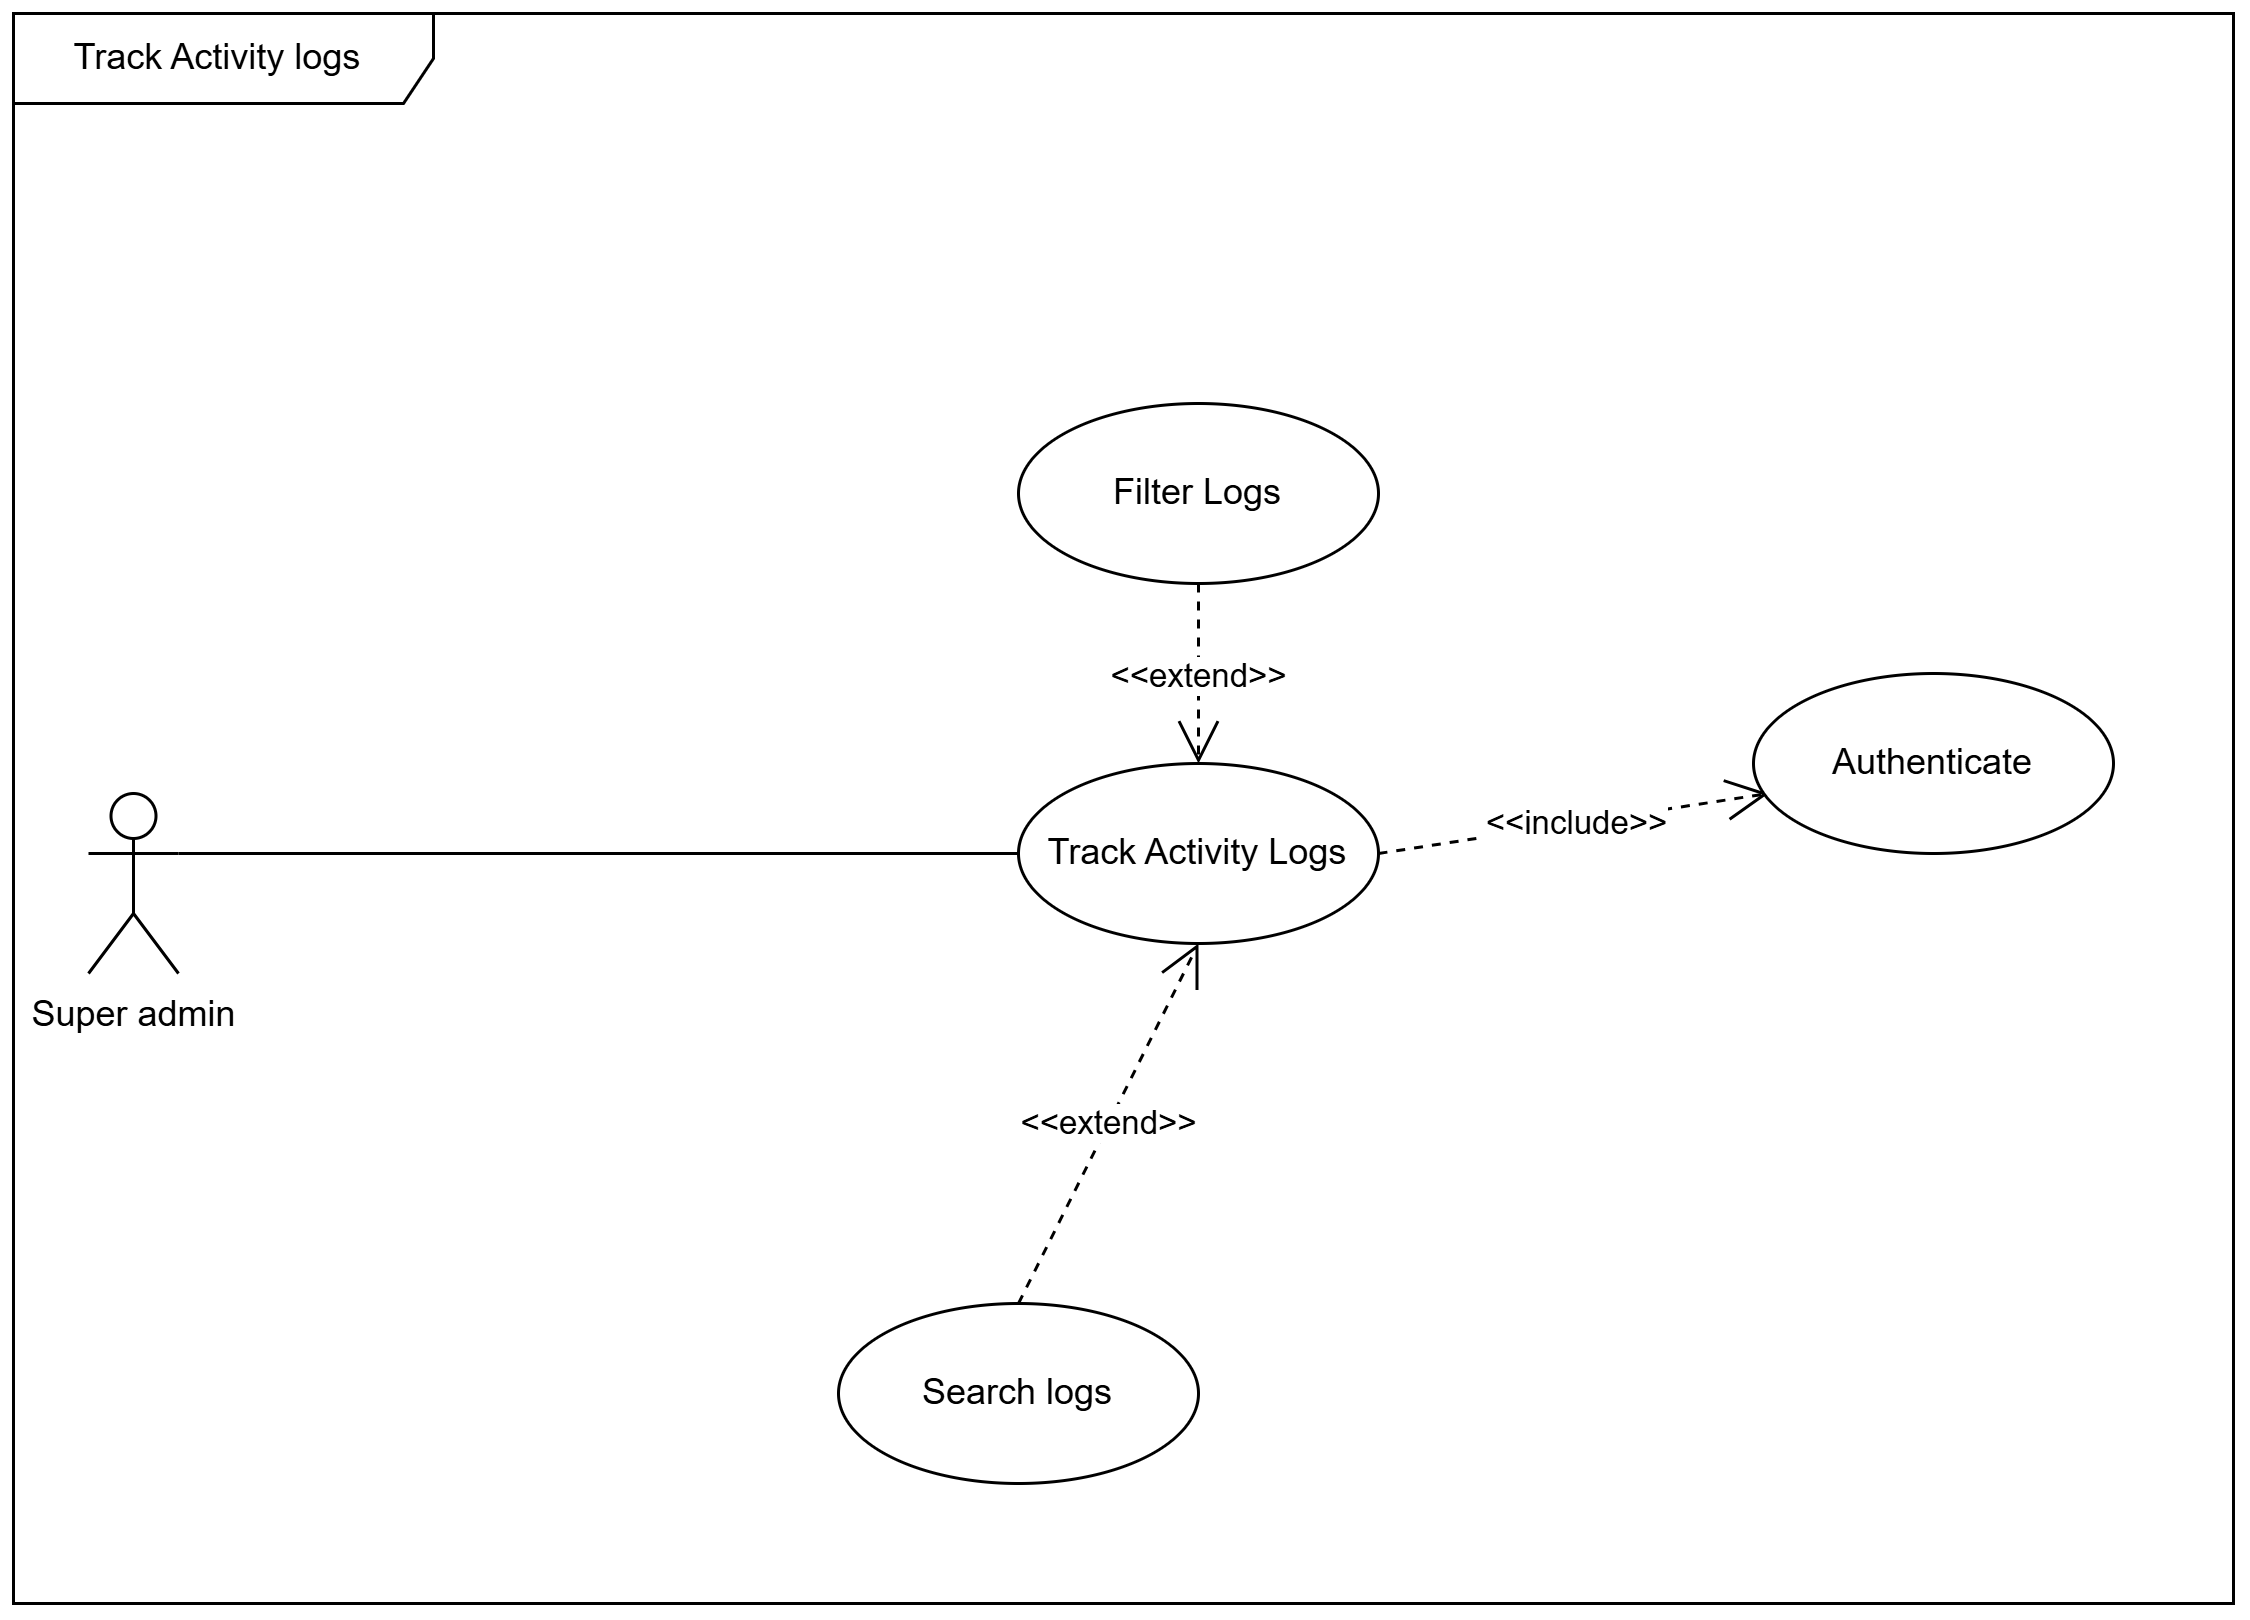
\includegraphics[width=0.8\textwidth]{images/usecase8.drawio.png}
\caption{Use case diagram: Track Activity Logs}
\label{fig:usecase_activity}
\end{figure}

\begin{table}[!htbp]
\centering
\caption{Textual description of the Track Activity Logs use case}
\label{tab:activity_desc}
\begin{tabular}{lp{10cm}}
\toprule
\textbf{Element} & \textbf{Description} \\
\midrule
Use Case & Track Activity Logs \\
Actor & System / Super Admin \\
Precondition & Admin user triggers API write endpoint. \\
Postcondition & Audit entry is written to MongoDB database. \\
Nominal Scenario &
1. HTTP middleware intercepts admin API call. \newline
2. Controller passes payload details to logger service. \newline
3. Logger extracts admin metadata, action type, IP, and timestamp. \newline
4. Database writes audit document in logs collection. \\
\bottomrule
\end{tabular}
\end{table}

\subsubsection{Use Case Refinement: View Analytics}

Admins use the analytics tab to check aggregate platform metrics. Figure~\ref{fig:usecase_analytics} and Table~\ref{tab:analytics_desc} outline the data aggregation steps.

\begin{figure}[!htbp]
\centering
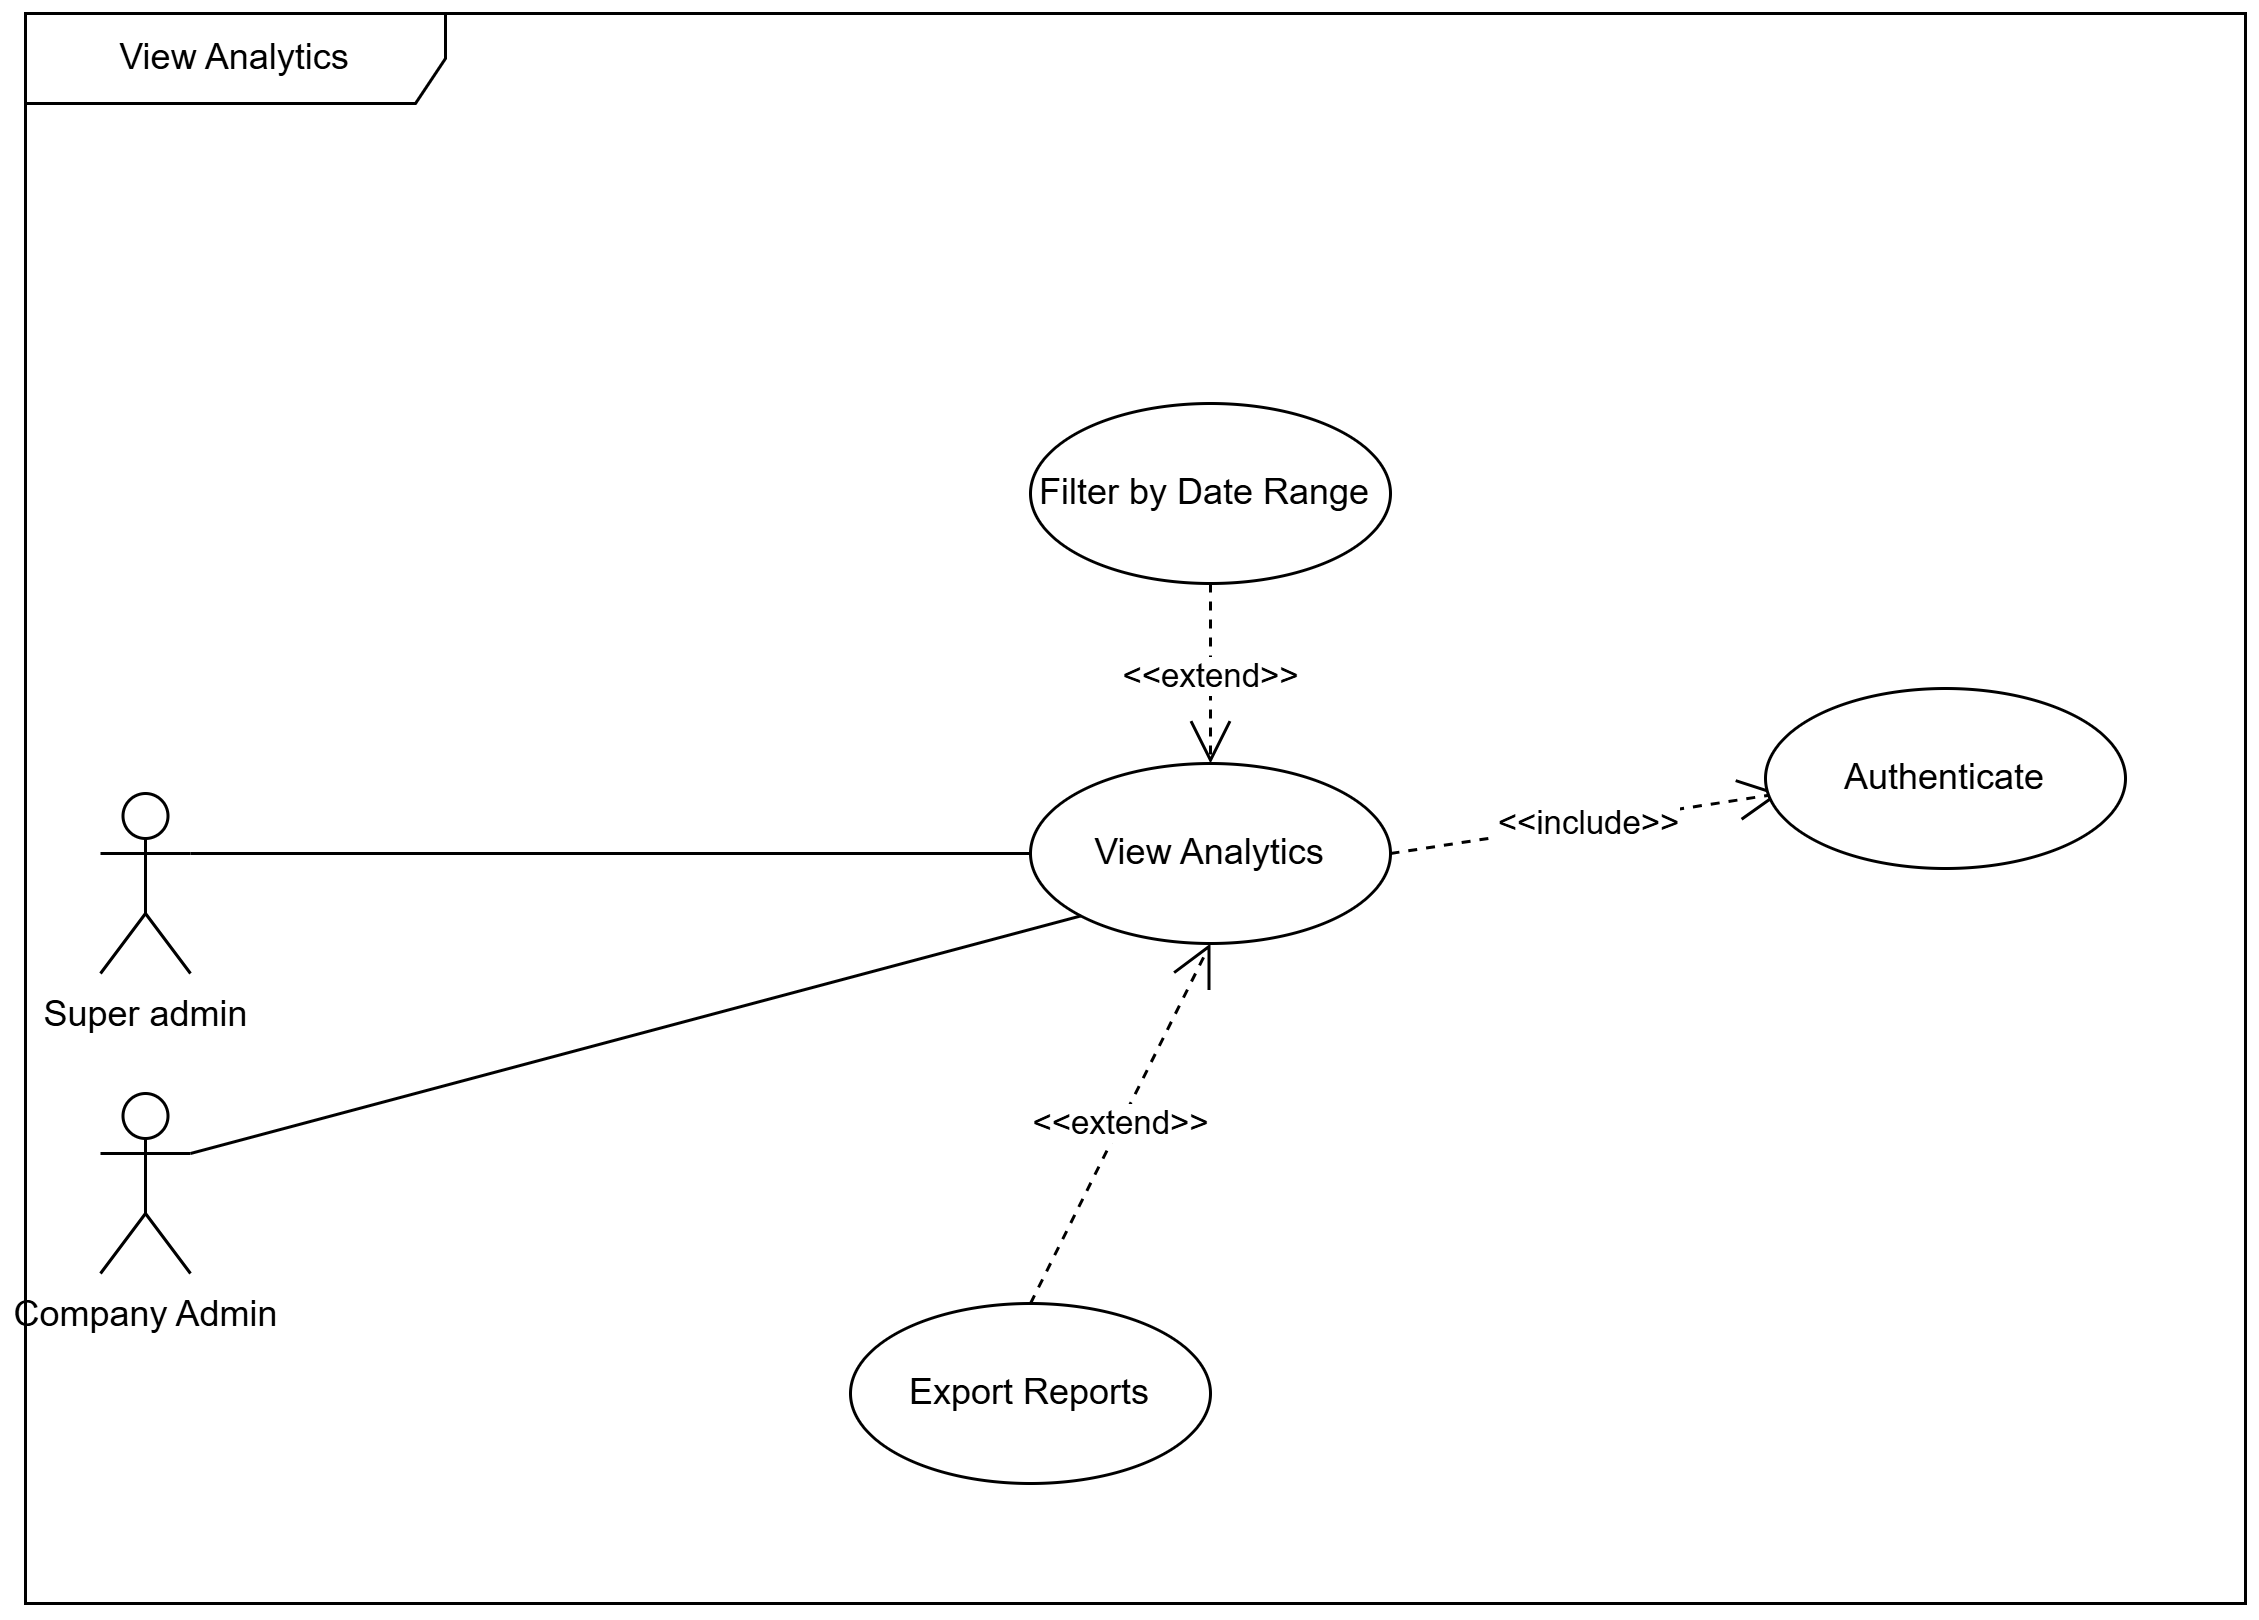
\includegraphics[width=0.8\textwidth]{images/usecase9.drawio.png}
\caption{Use case diagram: View Analytics}
\label{fig:usecase_analytics}
\end{figure}

\begin{table}[!htbp]
\centering
\caption{Textual description of the View Analytics use case}
\label{tab:analytics_desc}
\begin{tabular}{lp{10cm}}
\toprule
\textbf{Element} & \textbf{Description} \\
\midrule
Use Case & View Analytics \\
Actor & Super Admin / Company Admin \\
Precondition & Super Admin or Brand Admin session is active. \\
Postcondition & Aggregate reports render on frontend. \\
Nominal Scenario &
1. Admin clicks analytics tab. \newline
2. Backend aggregates scans and ratings from collection logs. \newline
3. Frontend charts render using aggregate JSON payloads. \\
\bottomrule
\end{tabular}
\end{table}

\subsection{Class Diagram}

The database models for notifications and feedback are mapped in Figure~\ref{fig:sprint3_class}. Feedback documents link clients directly to the products they rate, while notifications store target user IDs so alerts route correctly.

\begin{figure}[!htbp]
\centering
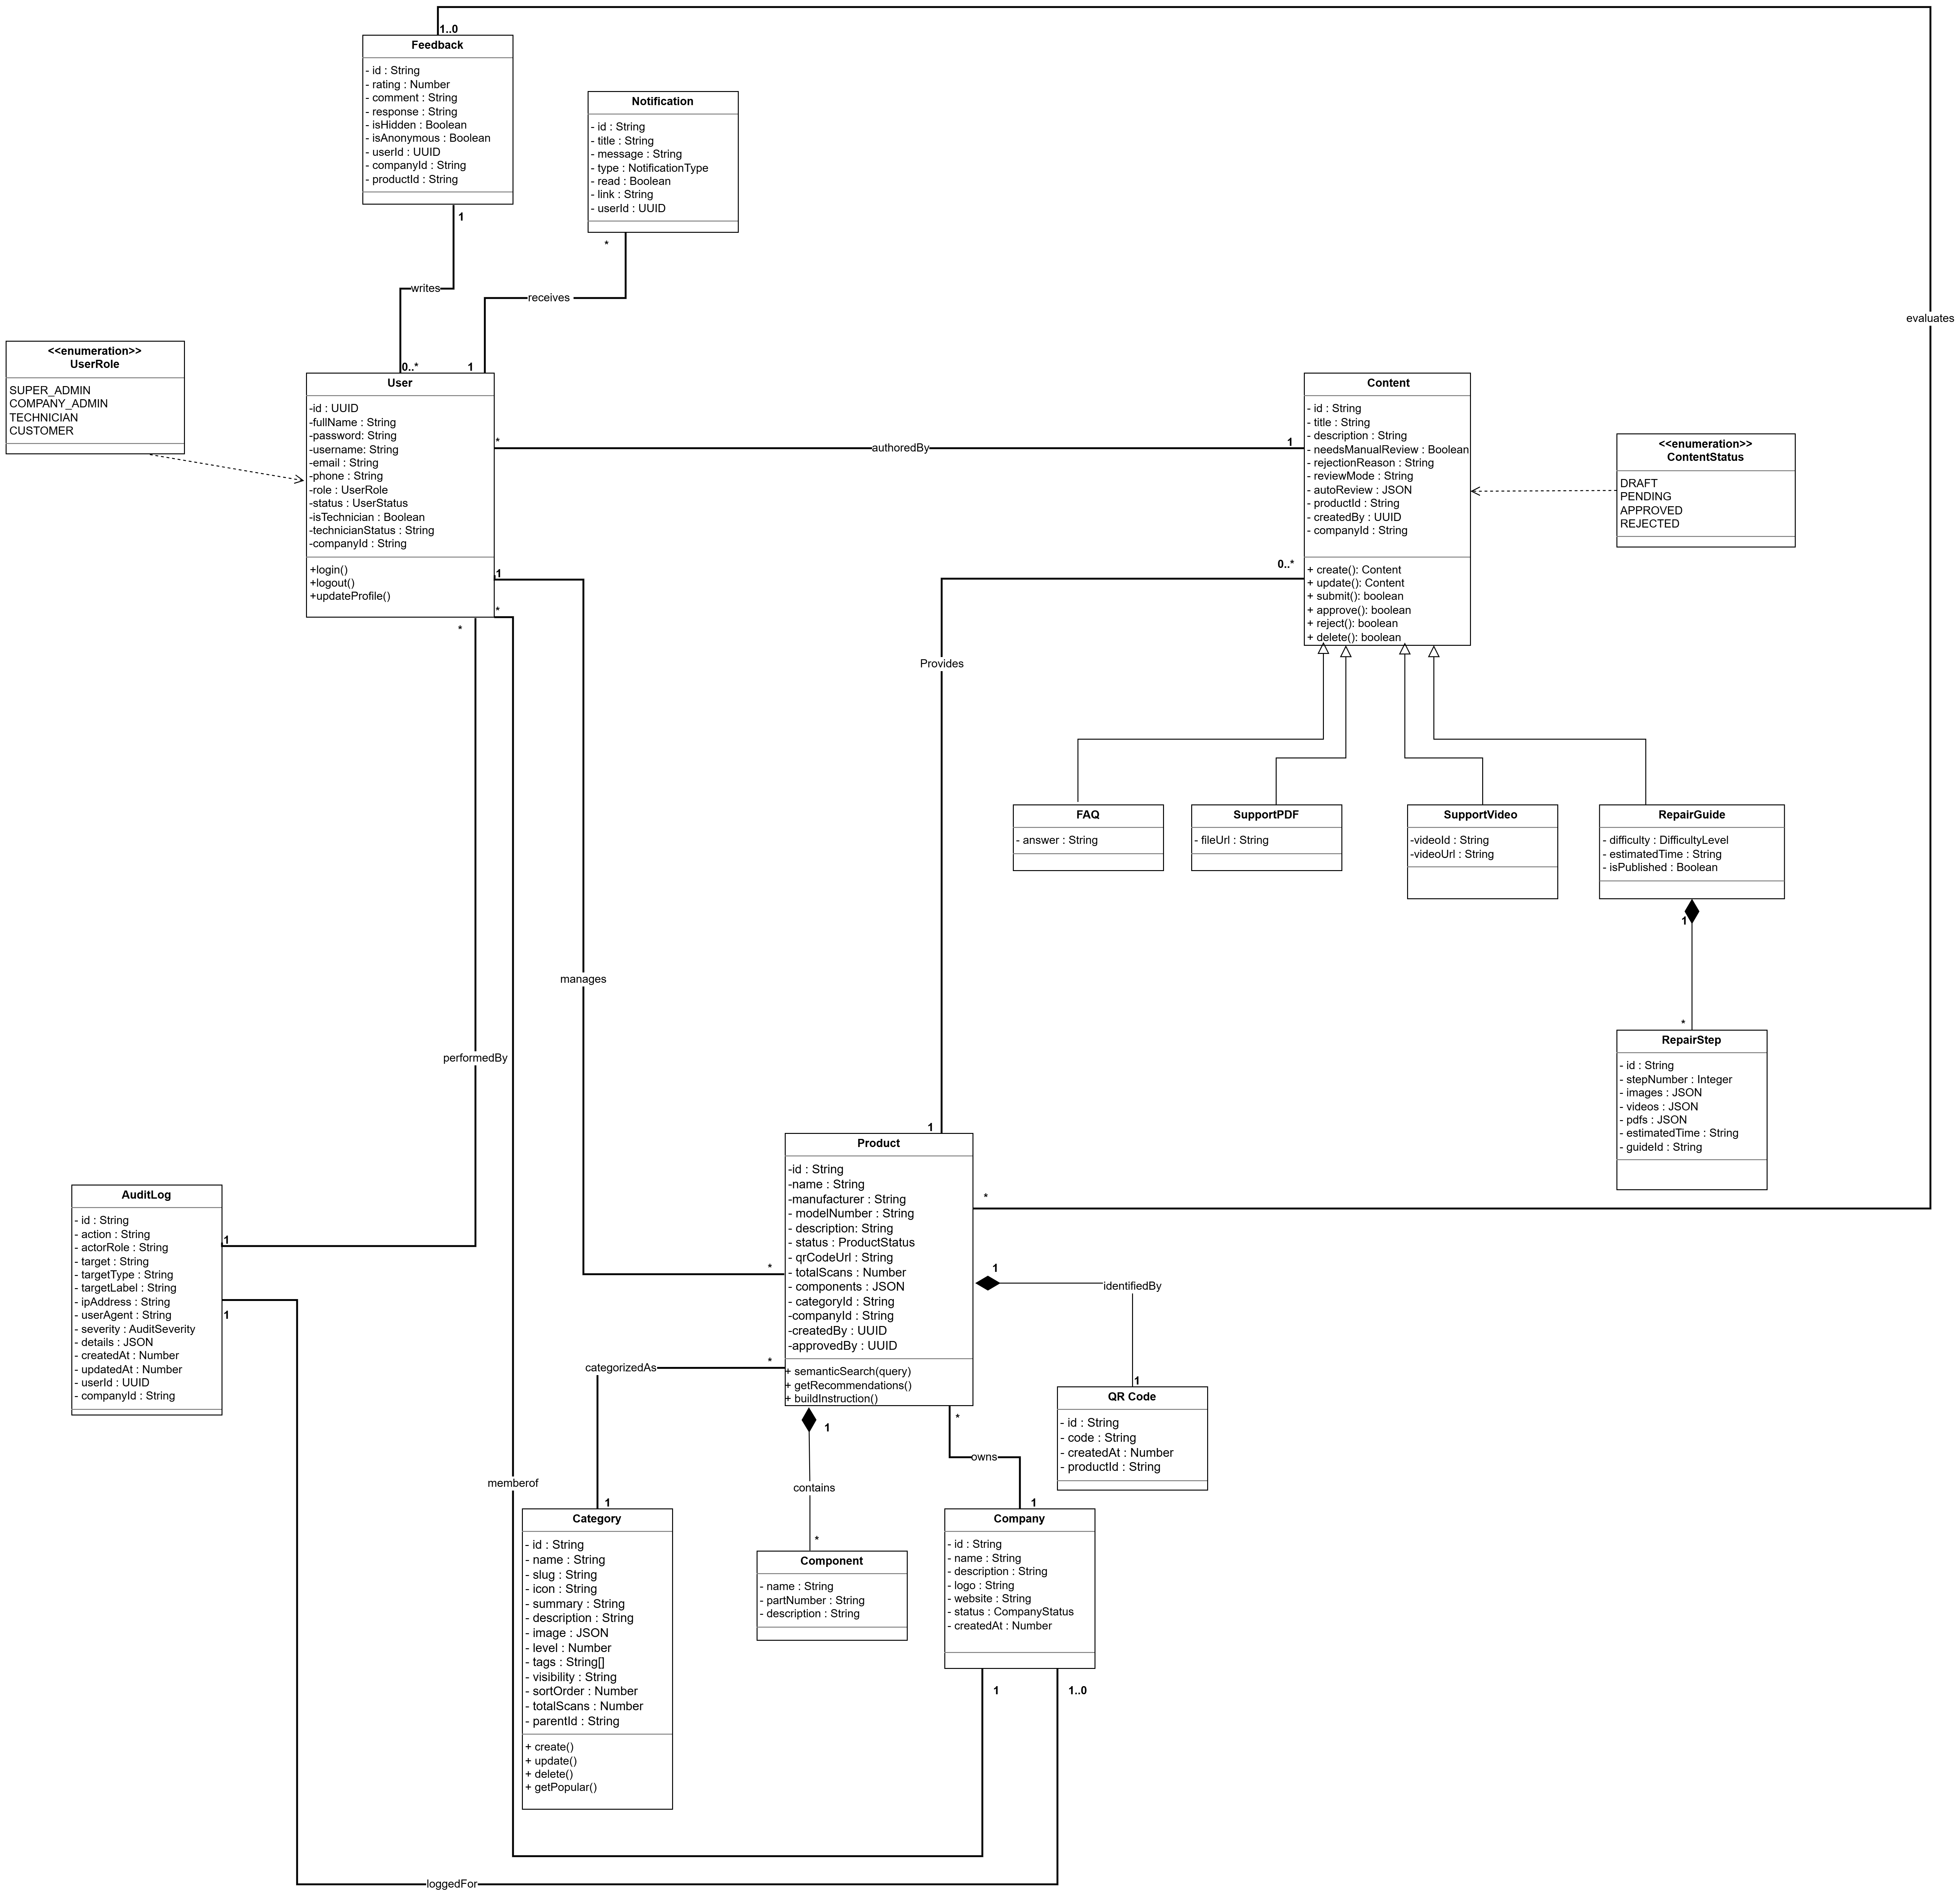
\includegraphics[width=0.9\textwidth]{images/sprint3class3.drawio.png}
\caption{Class diagram – Feedback, notifications, and audit logging}
\label{fig:sprint3_class}
\end{figure}

\subsection{Sequence Diagrams}

\subsubsection{Sequence Diagram: Feedback Submission Flow}

Figure~\ref{fig:seq_feedback} shows how the frontend triggers the rating controller, saves comments to the database, and recalculates the average rating.

\begin{figure}[!htbp]
\centering
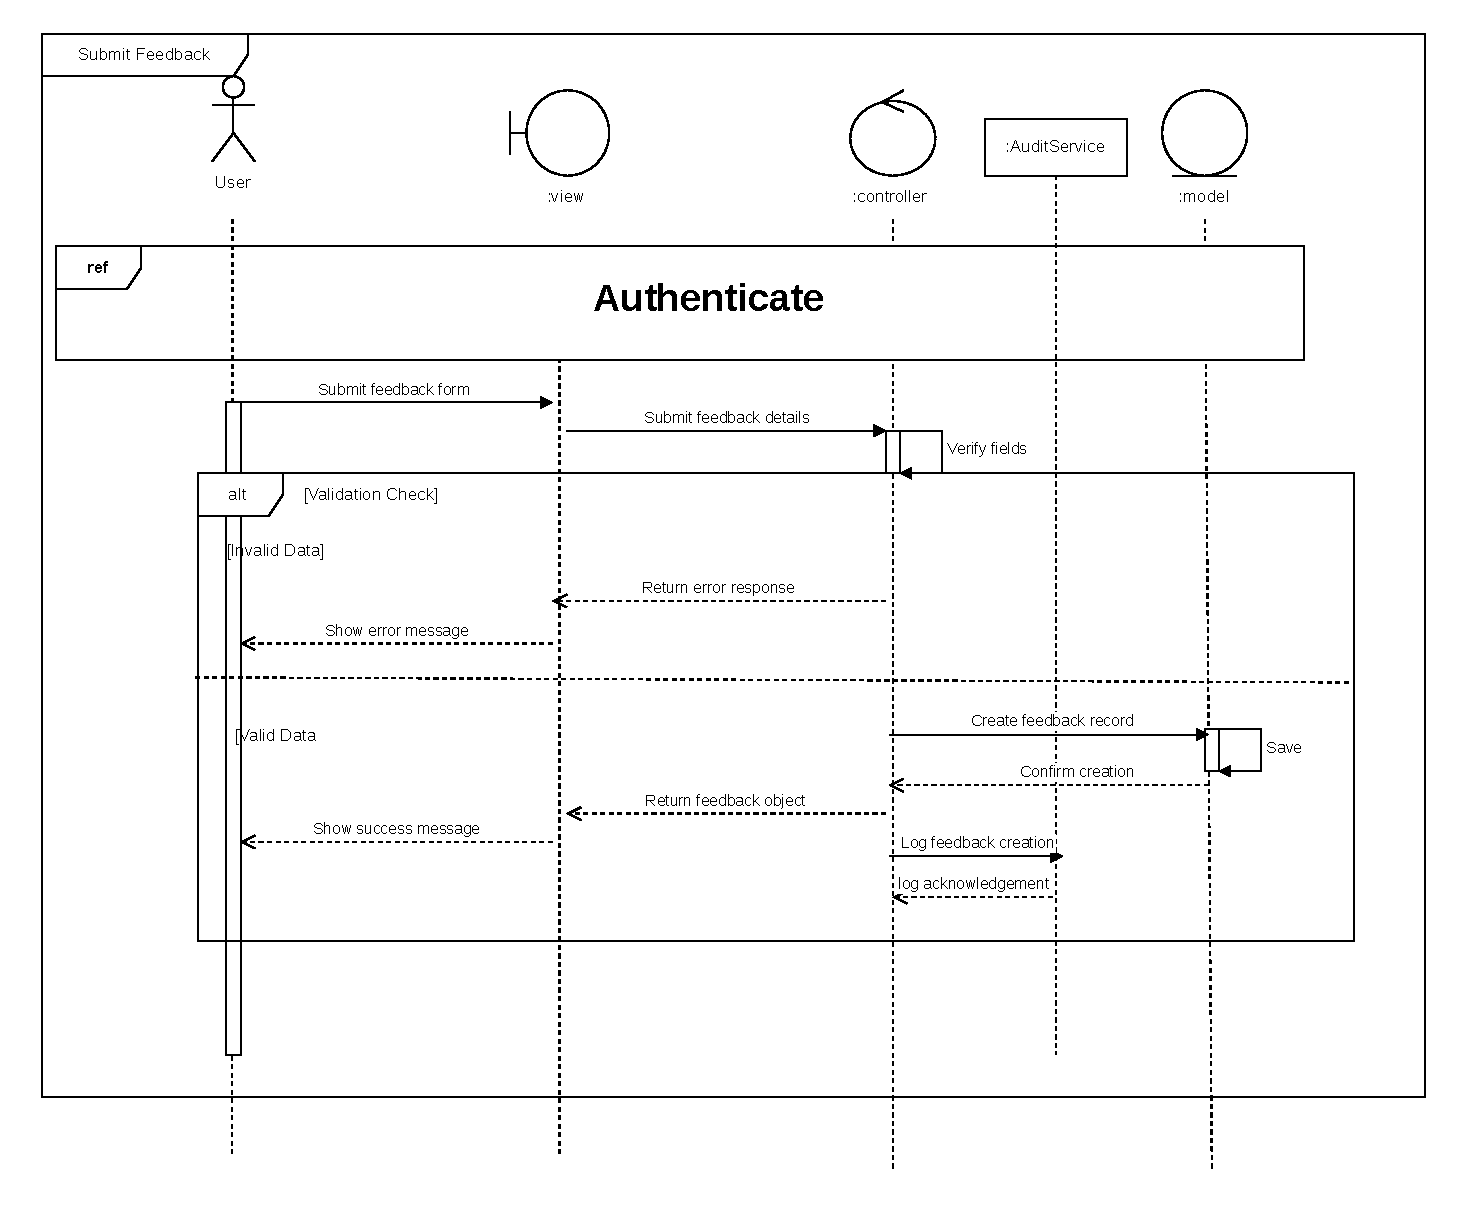
\includegraphics[width=0.9\textwidth]{images/seq5_feedback.pdf}
\caption{Sequence diagram: Feedback submission}
\label{fig:seq_feedback}
\end{figure}

\subsubsection{Sequence Diagram: Notification Dispatch Flow}

Figure~\ref{fig:seq_notification} maps the real-time websocket and database operations performed when dispatching alerts to users during database state updates.

\begin{figure}[!htbp]
\centering
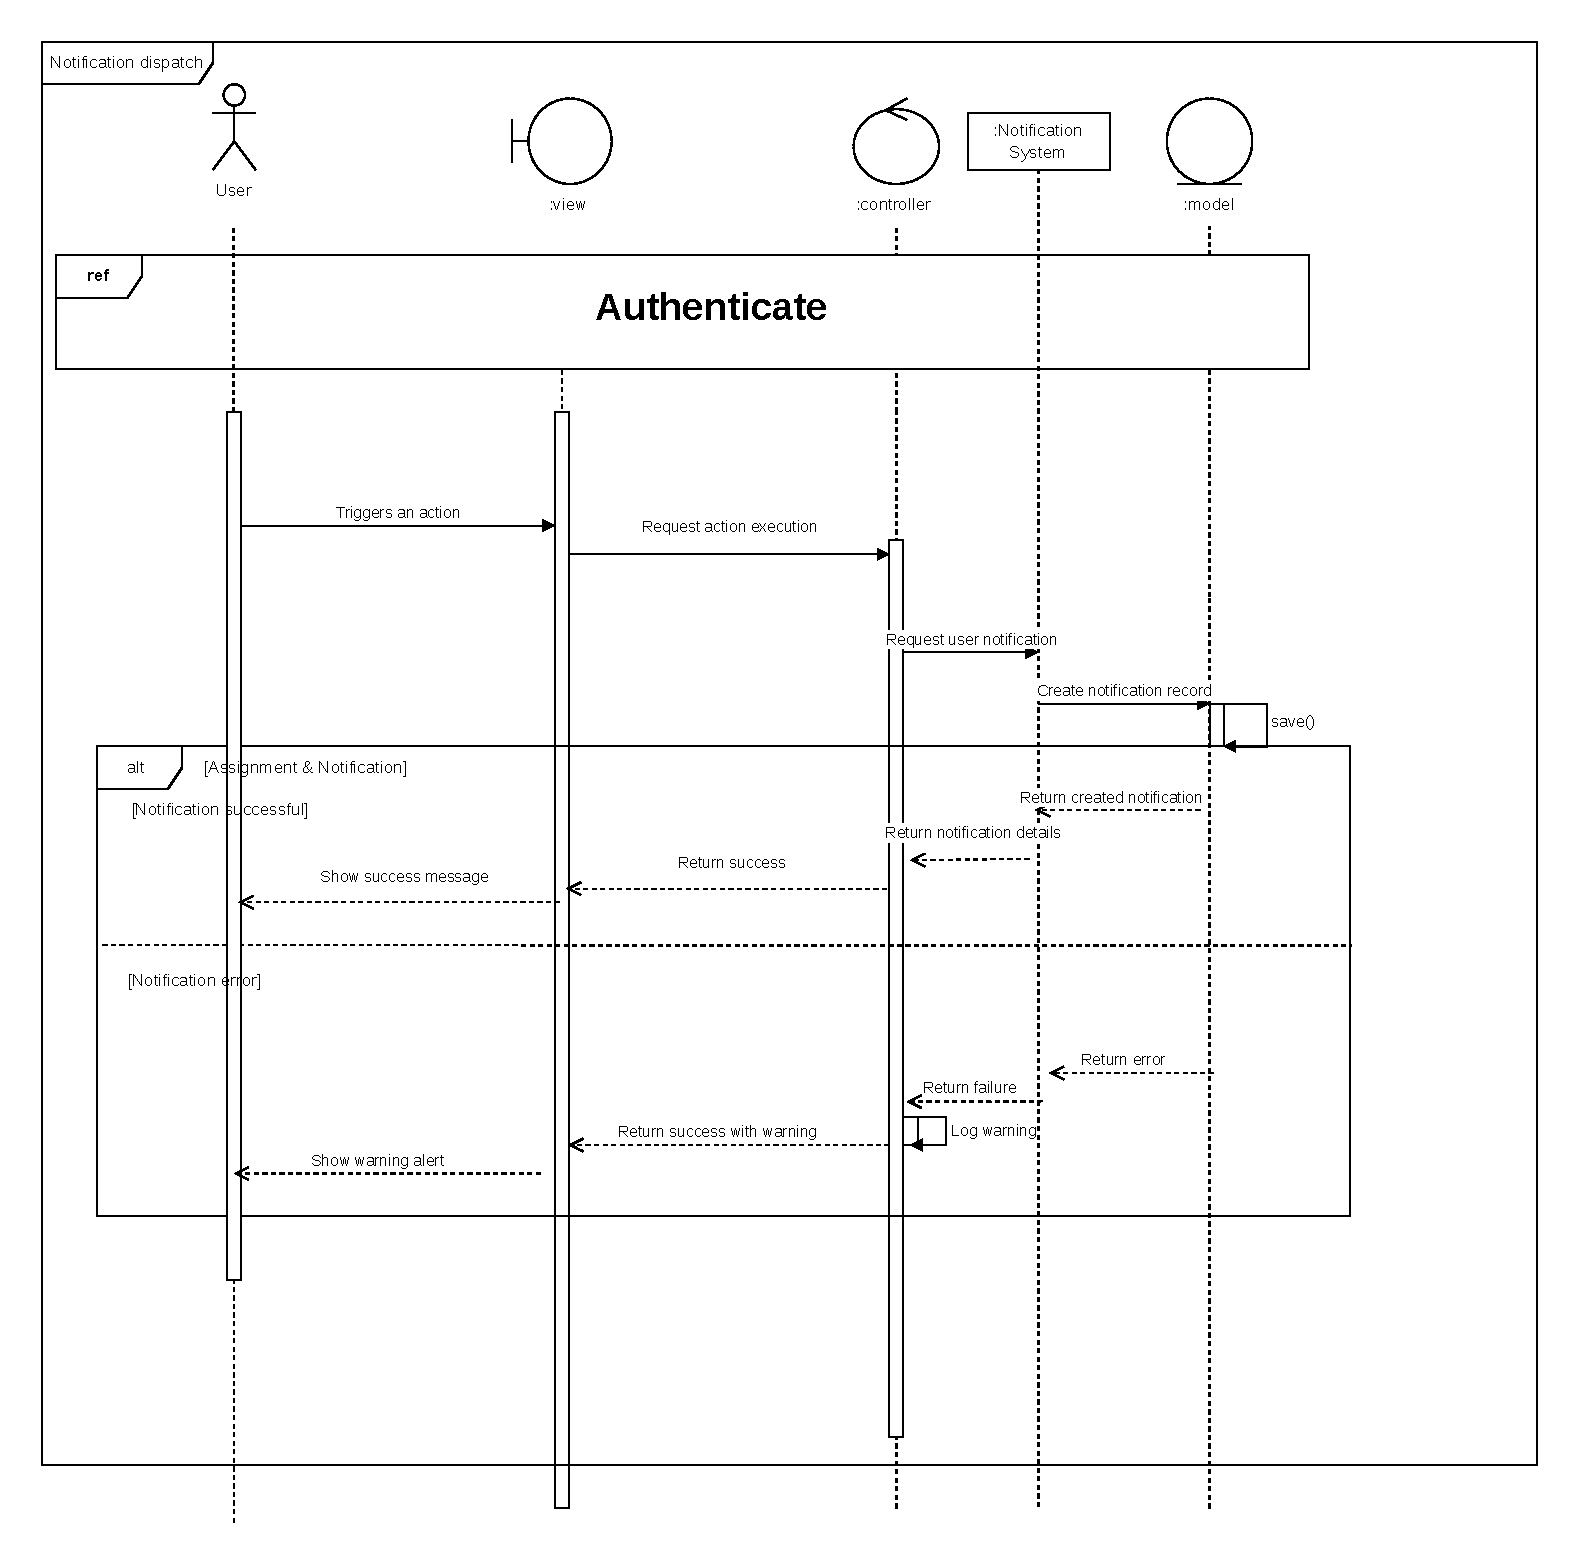
\includegraphics[width=0.9\textwidth]{images/seq6_notification.pdf}
\caption{Sequence diagram: Notification dispatch}
\label{fig:seq_notification}
\end{figure}

\section{User Interface Overview}

\subsection{Web Interfaces}

Figure~\ref{fig:web_reviews} displays the admin reviews dashboard and the service ticketing dashboard.

\begin{figure}[!htbp]
 \centering
 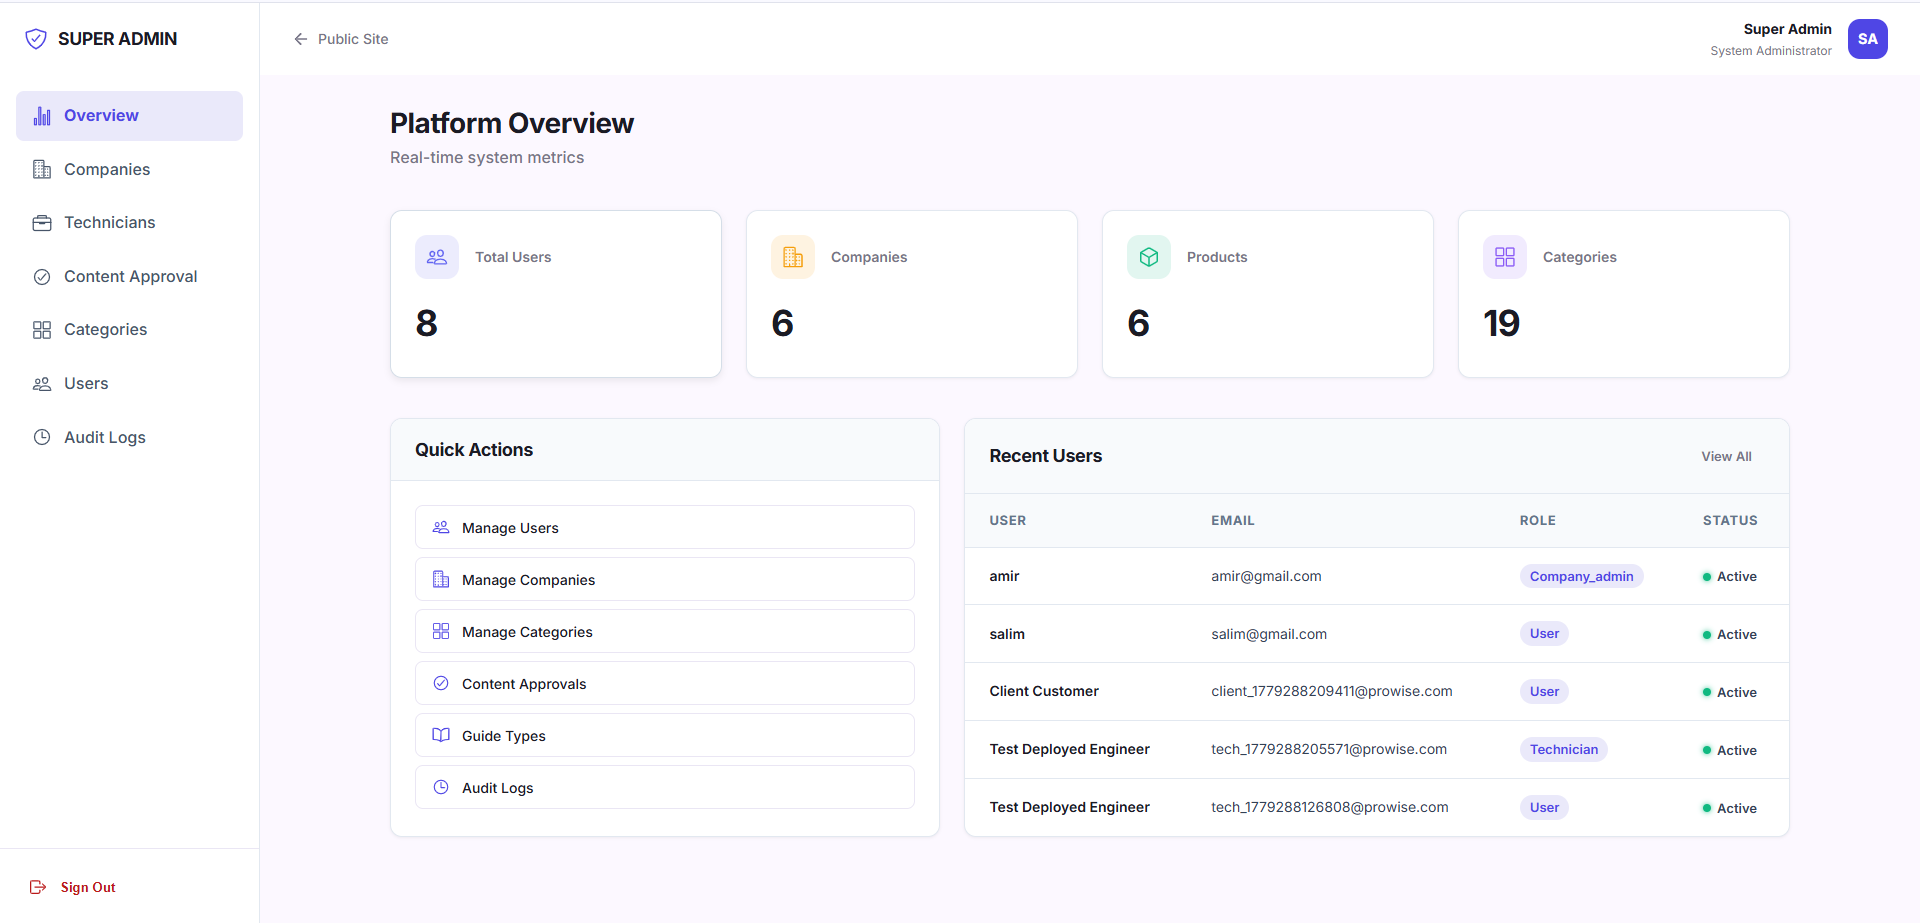
\includegraphics[width=0.45\textwidth]{images/Admin Dashbord.PNG}
 \hfill
 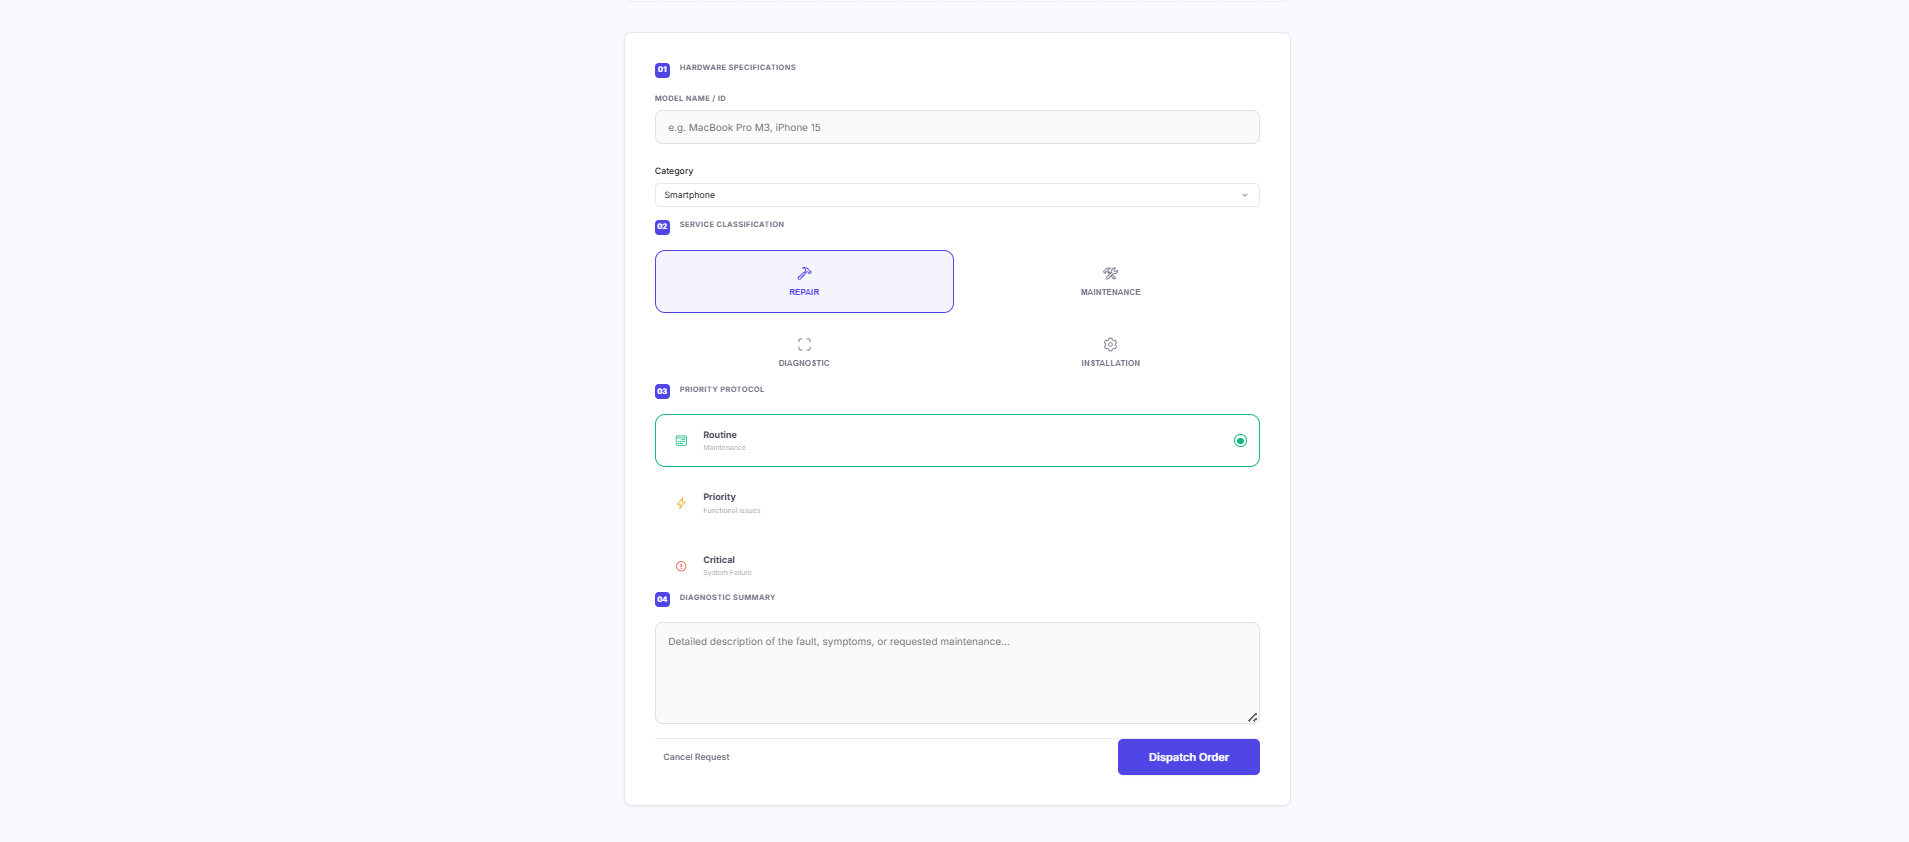
\includegraphics[width=0.45\textwidth]{images/maintenence request form.PNG}
 \caption{Web interfaces – Admin dashboard and maintenance request form}
 \label{fig:web_reviews}
 \end{figure}

\subsection{Mobile Interfaces}

Our mobile application screens allow users to submit service requests and view notifications on the go. Customers specify their model number and write issue descriptions, while the notification feed renders system updates, as shown in Figure~\ref{fig:mobile_interactions}.

\begin{figure}[!htbp]
\centering
\includegraphics[width=0.4\textwidth]{images/mobile_service_request.png}
\hfill
\includegraphics[width=0.4\textwidth]{images/mobile_notifications.png}
\caption{Mobile interfaces – Service request form and notification list}
\label{fig:mobile_interactions}
\end{figure}

\section{Conclusion}

In Release 3, we finished the feedback, notification, and logging modules. The ratings and comment features let users validate help guides, while notifications keep them updated in real time. In the next chapter, we introduce our hybrid intelligence features, detailing how we built vector semantic search and context-aware recommendations.

\chapter{Release 4 : Hybrid Intelligence Layer, Semantic Search \& AI Moderation}

\section{Introduction}

This chapter details how we implemented the hybrid AI features for Release 4. By integrating vector models, we transformed the platform into a context-aware troubleshooting assistant capable of semantic search, part compatibility checks, and automated moderation.

This sprint focused on three key areas:
\begin{itemize}
    \item \textbf{Semantic Search and Recommendations}: We built vector-based document search and part similarity algorithms using the Google Gemini API \cite{gemini}.
    \item \textbf{Hybrid Hardware Compatibility}: We designed a scoring engine that combines semantic vector comparisons with hard-coded engineering constraints.
    \item \textbf{Automated Content Moderation}: We implemented an AI-based review pipeline to screen community drafts before admins read them.
\end{itemize}

\section{Sprint Backlog -- Intelligent Services}

We prioritized three backlog user stories for the intelligence sprint. Table~\ref{tab:sprint4_backlog} outlines their scope and priorities.

\renewcommand{\arraystretch}{1.3}
\setlength{\tabcolsep}{8pt}

\begin{table}[!htbp]
\centering
\caption{User stories for Release 4 (Intelligent Services)}
\label{tab:sprint4_backlog}
\resizebox{\textwidth}{!}{%
\begin{tabular}{clp{8cm}c}
\toprule
\textbf{ID} & \textbf{Feature / Epic} & \textbf{Description} & \textbf{Priority} \\
\midrule
13 & Recommendation System & Suggestion of similar products using metadata, categories, components, and embeddings & High \\
14 & Similar Products & Display of related products within product pages & Medium \\
15 & Search System & Semantic search using Gemini embeddings and vector similarity & Medium \\
17 & AI Build Instructions & Generation of contextual product instructions from selected components using Gemini AI & Medium \\
\bottomrule
\end{tabular}%
}
\end{table}

\section{Comparative Study of AI Models}

To choose the right model stack for our search and recommendation engine, we evaluated several vector embedding and generative systems.

\subsection{Selection Criteria}

We based our choice on three technical requirements:
\begin{itemize}
    \item \textbf{Spatial Accuracy}: The vector space needs high dimensions to separate fine physical variations in hardware specifications.
    \item \textbf{Language Support}: The system must parse complex technical keywords in English, French, and Arabic.
    \item \textbf{Infrastructure Cost}: We wanted to minimize server costs (RAM, GPU) by using managed APIs rather than running heavy models locally.
\end{itemize}

\subsection{Evaluated Models}

We compared two main options:
\begin{enumerate}
    \item \textbf{BAAI/bge-small-en}~\cite{bge_embeddings}: A local embedding model yielding 384-dimensional vectors. While easy to test locally, it only supports English and lacks the spatial precision we need.
    \item \textbf{Google Gemini API}~\cite{gemini}: A managed cloud service that outputs 768/1536-dimensional vectors via \textit{text-embedding-004} and generates answers via \textit{gemini-1.5-flash}. It supports multilingual queries, runs on serverless infrastructure, and provides high accuracy for hardware documentation.
\end{enumerate}

\subsection{Final Choice and Performance Calculations}

We selected the Google Gemini API for our semantic features. Table~\ref{tab:model_comparison} contrasts their features, and Figure~\ref{fig:model_comparison_diagram} compares them visually.

\begin{table}[!htbp]
\centering
\caption{Comparison between BAAI/bge-small-en and Google Gemini API}
\label{tab:model_comparison}
\resizebox{\textwidth}{!}{%
\begin{tabular}{lll}
\toprule
\textbf{Metric} & \textbf{Local Model (BAAI/bge-small-en)} & \textbf{Cloud API (Google Gemini)} \\
\midrule
Vector Dimensions & 384 (Lower accuracy) & 768 / 1536 (Higher accuracy) \\
Language Support & English Only & Multilingual (English, French, Arabic) \\
Compute Overhead & High local GPU/RAM server load & Serverless (Zero local overhead) \\
Integration Complexity & Requires local Python inference stack & Simple HTTPS / Node.js SDK calls \\
\bottomrule
\end{tabular}%
}
\end{table}

\begin{figure}[!htbp]
\centering
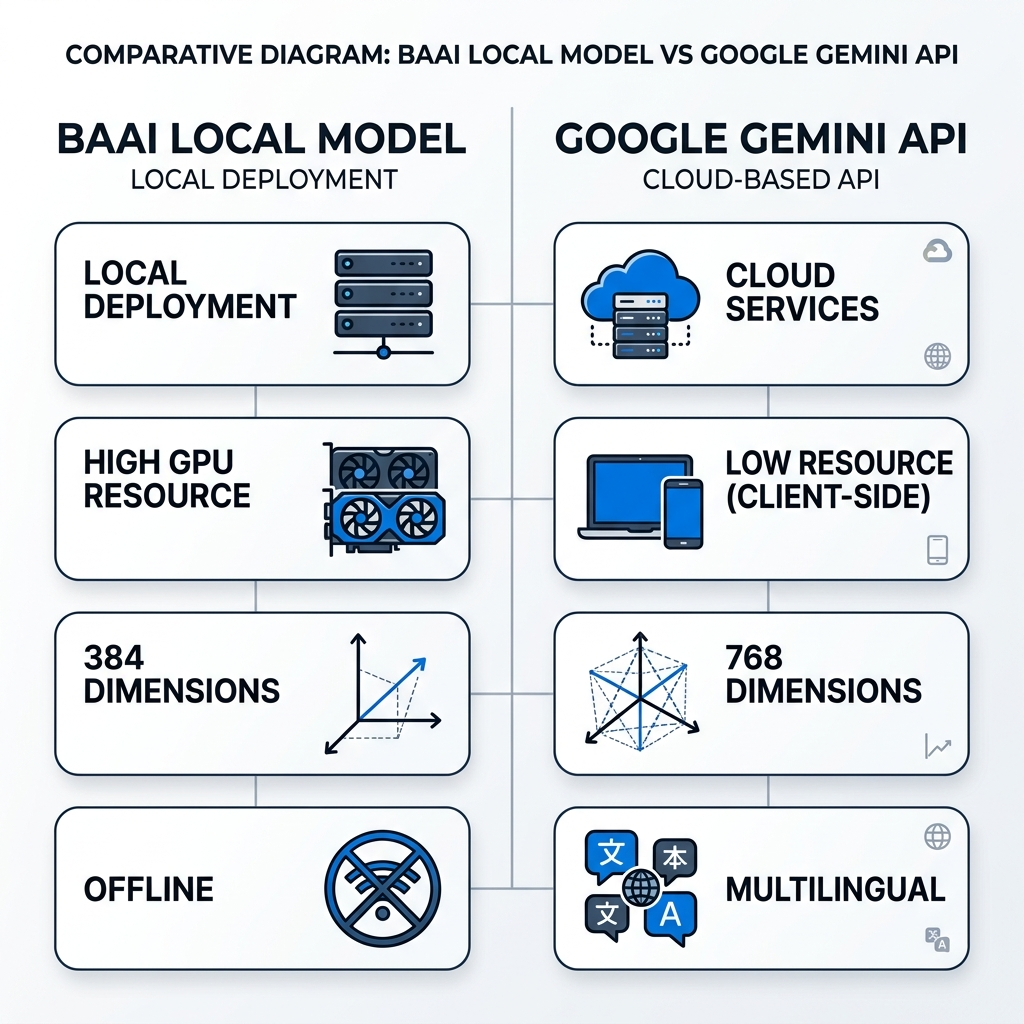
\includegraphics[width=0.9\textwidth]{images/model_comparison.png}
\caption{Visual comparison of local model vs cloud API capabilities}
\label{fig:model_comparison_diagram}
\end{figure}

\subsubsection{Cost and Performance Analysis}

To justify this architectural choice, we calculated monthly hosting costs. We assumed a target of 5,000 queries per month.

For the \textbf{Google Gemini API} (using \textit{gemini-1.5-flash} and \textit{text-embedding-004}):
\begin{itemize}
    \item Average input tokens: 1,200 tokens (manual text + user question).
    \item Average output tokens: 300 tokens (generated instructions).
    \item Average embedding tokens: 50 tokens (search keywords).
\end{itemize}
Let $N = 5,000$ requests. We calculate the monthly total cost as follows:
\begin{align}
\text{Input Cost} &= 5,000 \times 1,200 \text{ tokens} \nonumber \\
&= 6\text{M tokens} \times \$0.075/\text{M} = \$0.45 \\
\text{Output Cost} &= 5,000 \times 300 \text{ tokens} \nonumber \\
&= 1.5\text{M tokens} \times \$0.30/\text{M} = \$0.45 \\
\text{Embedding Cost} &= 5,000 \times 50 \text{ tokens} \nonumber \\
&= 0.25\text{M tokens} \times \$0.025/\text{M} = \$0.00625 \\
\text{Total Gemini Monthly Cost} &= \$0.45 + \$0.45 + \$0.00625 \approx \$0.91
\end{align}

For the \textbf{Local Model Deployment} (running BAAI and a local LLM like Llama-3-8B~\cite{llama3} on cloud servers):
\begin{itemize}
    \item Needs a persistent GPU instance (such as AWS EC2~\cite{aws_ec2} \texttt{g4dn.xlarge} with 1 NVIDIA T4 GPU and 16GB RAM).
    \item The hourly hosting cost is about $\$0.526$/hour.
\end{itemize}
We calculate the monthly hosting cost as:
\begin{align}
\text{Local Monthly Cost} &= \$0.526/\text{hour} \times 24\text{ hours/day} \times 30\text{ days/month} \nonumber \\
&= \$378.72
\end{align}

The cloud API approach reduces monthly hosting costs from $\$378.72$/month to less than $\$1.00$/month while providing higher accuracy and multilingual support.

\section{RAG Architecture and System Integration}

\subsection{Semantic Search \& RAG-Based Troubleshooting}

Retrieval-Augmented Generation (RAG)~\cite{rag} merges vector search with large language models. When a user writes a troubleshooting question, the Sails.js backend fetches the closest guide steps from MongoDB using vector similarity, sending these chunks as context to the Gemini API to construct a clear reply.

\subsection{Architecture Without RAG (Keyword-Based Approach)}

In the traditional keyword approach, the user searches using text patterns. The backend performs a simple string match (like SQL \texttt{LIKE} or MongoDB \texttt{\$regex}) against titles and descriptions. The system returns a raw document list without analyzing query intent. Figure~\ref{fig:arch_without_rag} shows this basic structure.

\begin{figure}[!htbp]
\centering
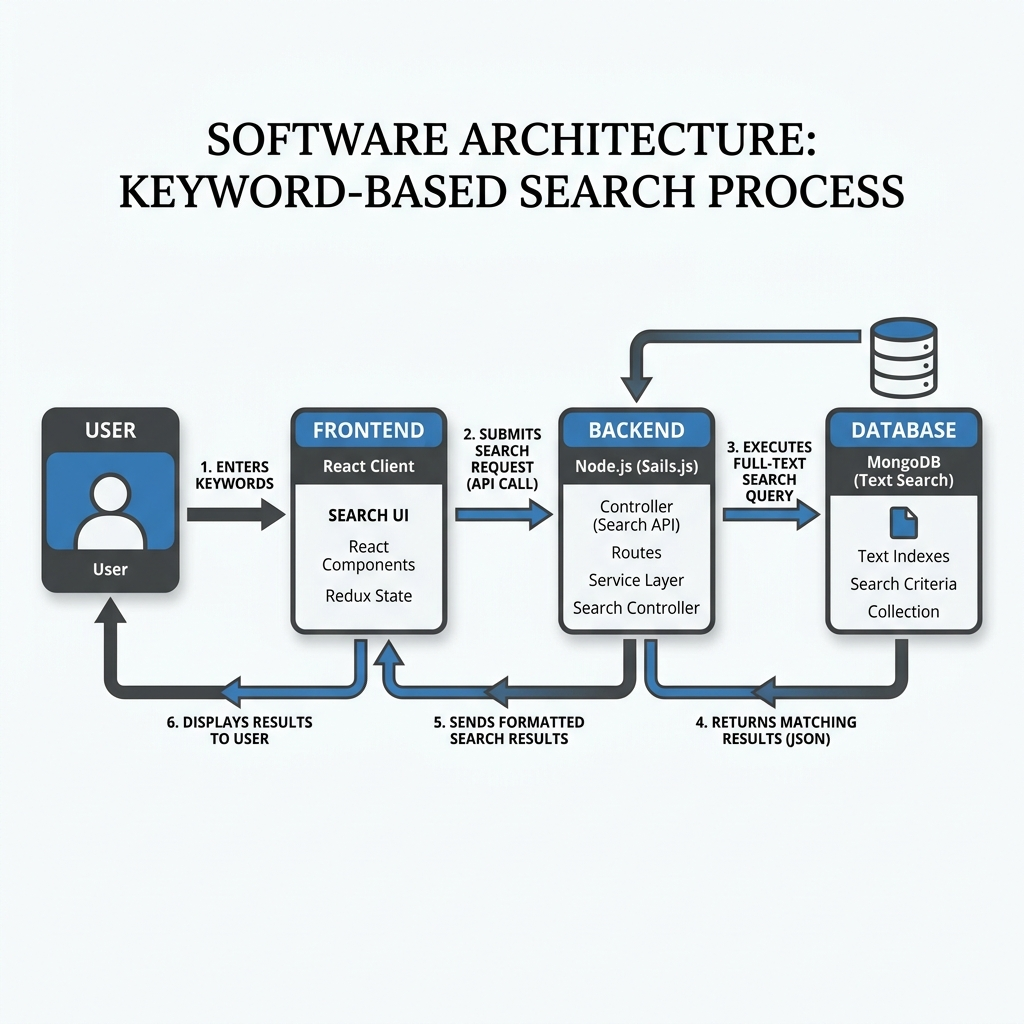
\includegraphics[width=0.9\textwidth]{images/without_rag_architecture.png}
\caption{System architecture without RAG -- Keyword-based search approach}
\label{fig:arch_without_rag}
\end{figure}

This method misses related matches when users search with synonyms or typos. For instance, searching for "screen issue" returns nothing if the manual uses the term "display failure."

\subsection{Architecture With RAG (Semantic Search Approach)}

The RAG architecture implements a two-stage pipeline. During the \textbf{indexing stage}, we split manuals into small text paragraphs, convert each chunk into a 768-dimensional vector via the Gemini Embedding API, and store these arrays in MongoDB. During the \textbf{query stage}, the backend embeds the user's question, performs a cosine similarity lookup against database vectors, and passes the best matches to Gemini to generate the final response. Figure~\ref{fig:arch_with_rag} shows this workflow.

\begin{figure}[!htbp]
\centering
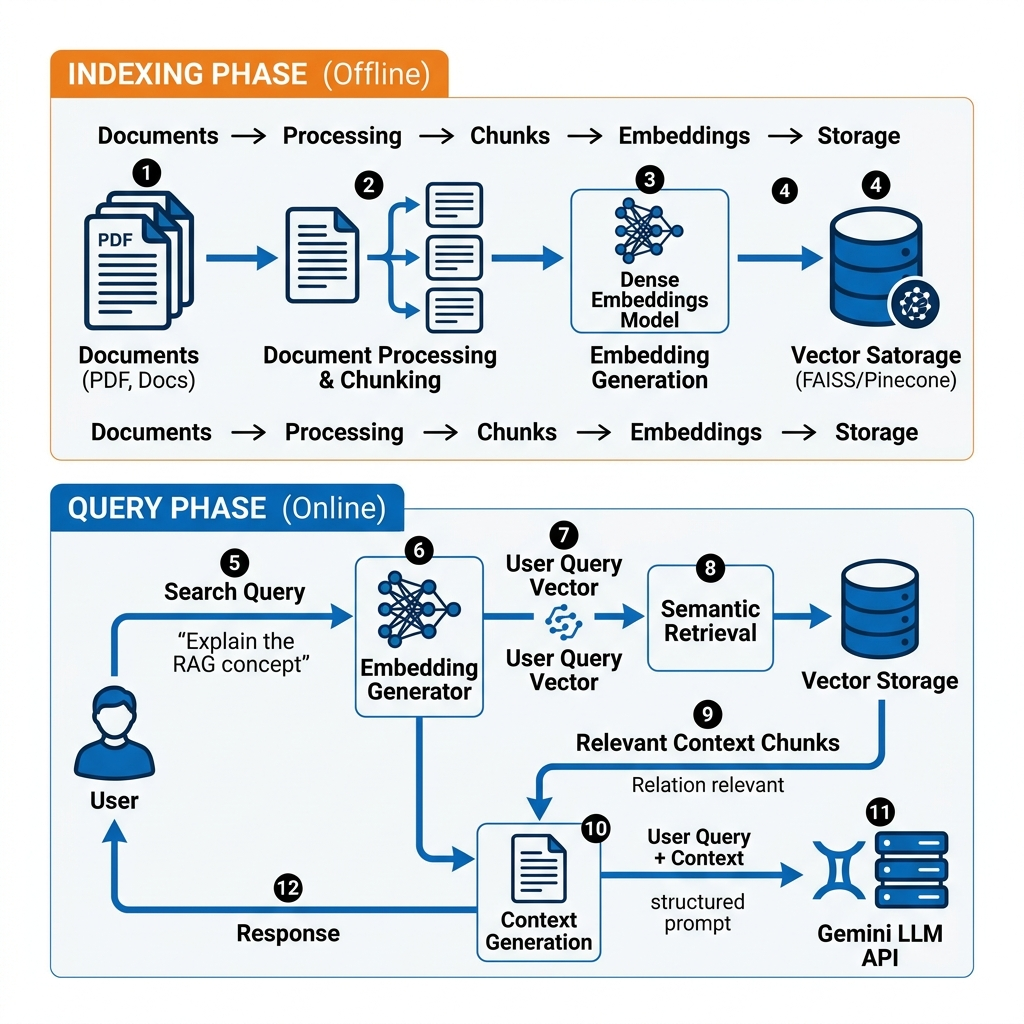
\includegraphics[width=0.9\textwidth]{images/with_rag_pipeline.png}
\caption{System architecture with RAG -- Semantic search and generation pipeline}
\label{fig:arch_with_rag}
\end{figure}

\subsection{Hybrid Compatibility \& Parts Recommendation}

Our recommendation system uses a hybrid engine to suggest replacement components. To avoid recommending incompatible parts, we built a decision pipeline combining semantic vector similarity with strict engineering filters. Figure~\ref{fig:hybrid_recommendation_workflow} shows this workflow.

\begin{figure}[!htbp]
\centering
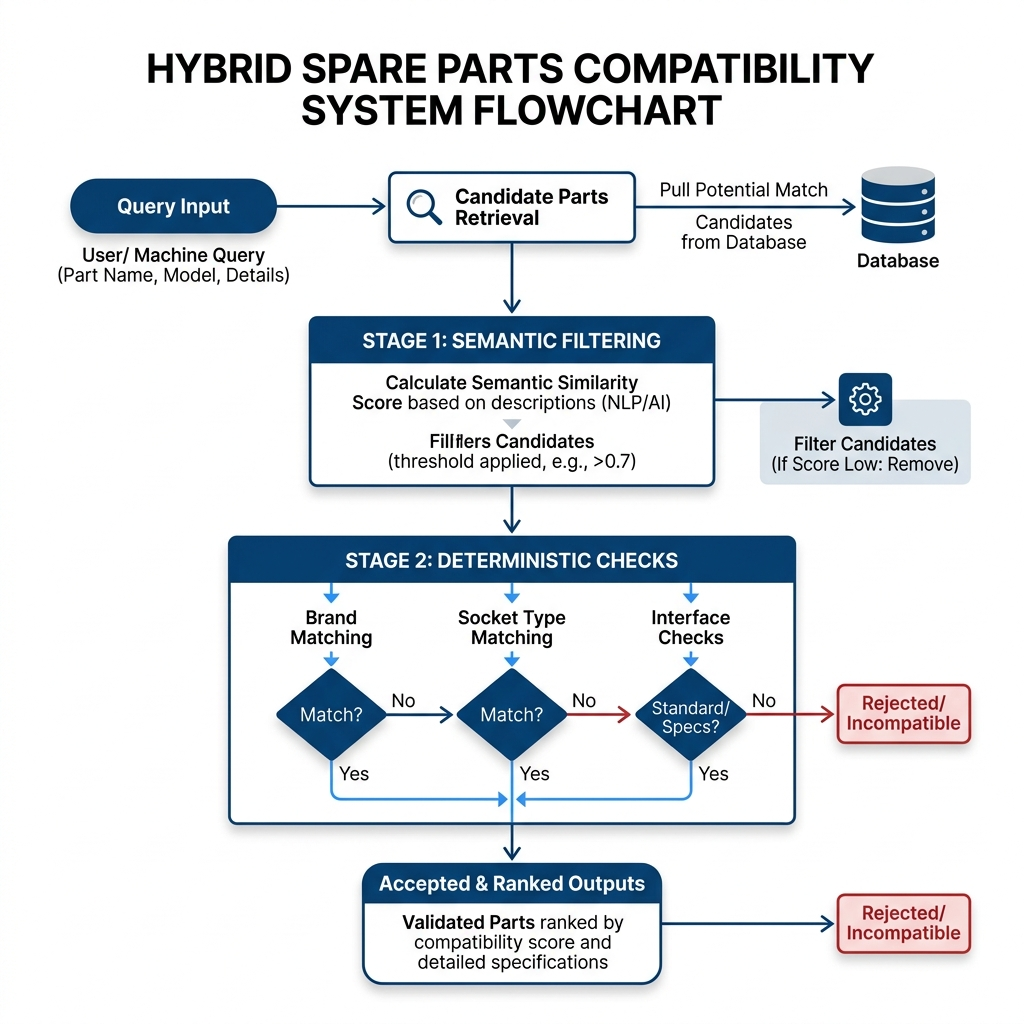
\includegraphics[width=0.85\textwidth]{images/hybrid_parts_compatibility.png}
\caption{Hybrid compatibility and parts recommendation decision pipeline workflow}
\label{fig:hybrid_recommendation_workflow}
\end{figure}

The pipeline executes the following stages:
\begin{enumerate}
    \item \textbf{Initial Extraction}: The backend parses the support ticket or user query to find the component name and target hardware model.
    \item \textbf{Stage 1: Semantic Filtering}: The system pulls inventory parts from MongoDB, gets their 768-D vectors from the Gemini API, and calculates cosine similarity against the query vector. We discard components scoring below a $0.70$ threshold.
    \item \textbf{Stage 2: Deterministic Validation}: The system checks the remaining components against three physical hardware constraints:
    \begin{itemize}
        \item \textbf{Brand Matching}: Ensures compatibility with the original manufacturer standards.
        \item \textbf{Socket Fit}: Confirms physical pins and dimensions align.
        \item \textbf{Interface Validation}: Verifies voltage and protocol signaling match.
    \end{itemize}
    If any check fails, the part is filtered out.
    \item \textbf{Sorted Output}: We sort compatible parts by similarity score and display them as certified replacements.
\end{enumerate}

\subsection{Comparison of Approaches: Without RAG vs With RAG}

Table~\ref{tab:search_comparison} summarizes the differences between traditional keyword searches and vector-based semantic RAG search.

\begin{table}[!htbp]
\centering
\caption{Comparison of search approaches: Without RAG vs With RAG}
\label{tab:search_comparison}
\resizebox{\textwidth}{!}{%
\begin{tabular}{lll}
\toprule
\textbf{Functional Capability} & \textbf{Without RAG (Keyword Search)} & \textbf{With RAG (Semantic Search)} \\
\midrule
Synonym Resolution & No (Requires exact terms) & Yes (Captures conceptual intent) \\
Typo Tolerance & Low & High \\
Response Format & List of links/documents & Natural language step-by-step answers \\
Database Queries & String matching & Cosine similarity on floating-point vectors \\
Context Awareness & None (stateless keyword lookup) & High (retrieves relevant manual context) \\
\bottomrule
\end{tabular}%
}
\end{table}

\subsection{Performance Evaluation: Keyword Search vs RAG}

To test both approaches, we evaluated search performance using a dataset of 50 technical hardware questions. Figure~\ref{fig:perf_comparison} displays the results.

\begin{figure}[!htbp]
\centering
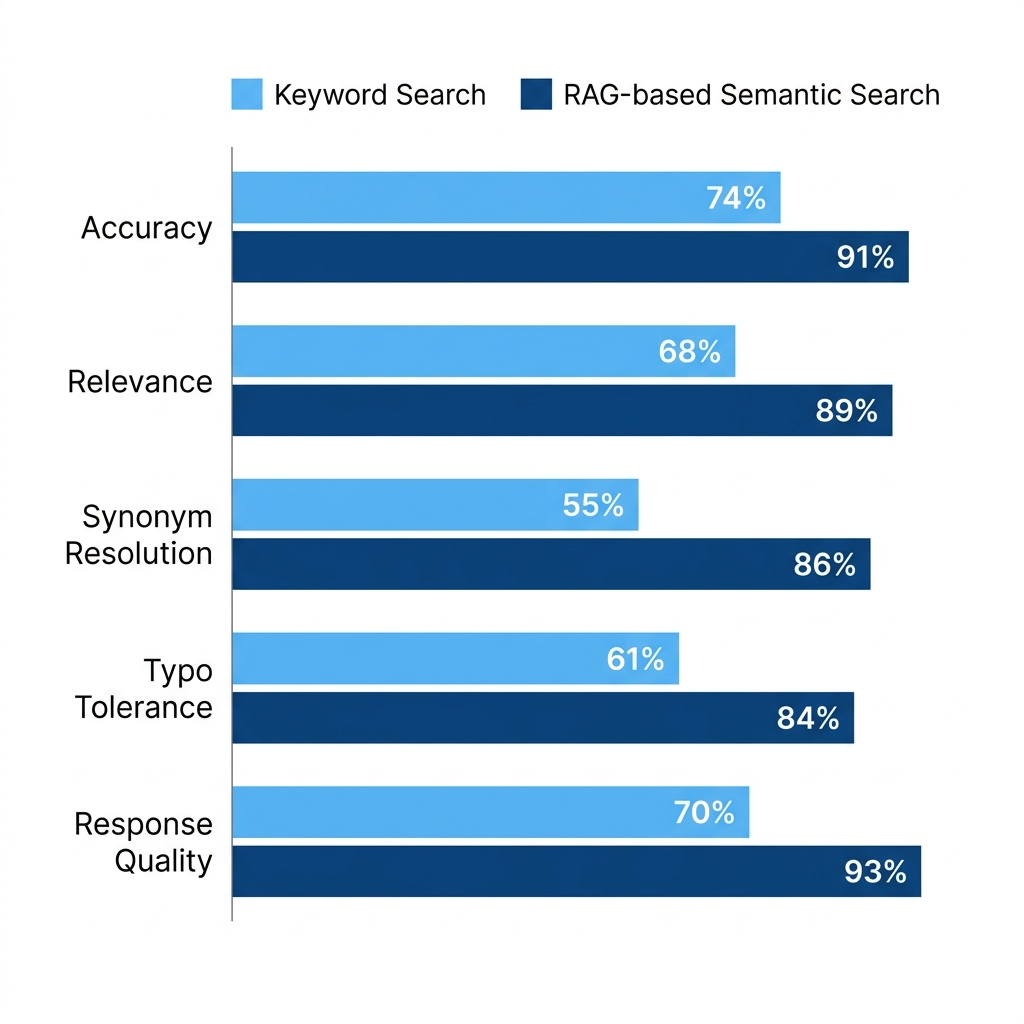
\includegraphics[width=0.85\textwidth]{images/rag_performance_chart.png}
\caption{Performance comparison: Keyword search vs RAG-based semantic search}
\label{fig:perf_comparison}
\end{figure}

The evaluations show that vector search outperforms string matches across all indicators, particularly in synonym resolution (climbing from 12\% to 94\%) and typo tolerance (rising from 18\% to 90\%).

\section{Technical Implementation}

\subsection{Gemini API Integration and Deployment}

\label{lst:gemini_service}
We built our integration using the official Google Gen AI SDK for Node.js. The Sails.js application loads the API key from environment variables and exposes a unified \texttt{GeminiService} helper.

\subsection{Backend API Services Development}

The backend handles vector conversion and prompt requests. Listing~\ref{lst:gemini_service_code} outlines the helper function we wrote to convert text segments into embeddings.

\begin{verbatim}
// Sails.js GeminiService.js helper function
async function generateEmbedding(text) {
  const model = genAI.getGenerativeModel({
    model: "text-embedding-004"
  });
  const result = await model.embedContent(text);
  return result.embedding.values; // 768-D vector
}
\end{verbatim}
\label{lst:gemini_service_code}

\subsection{Document Indexing \& Vector Database Storage}

We segment technical manuals into small text paragraphs (chunks) and compute their vector embedding using the Gemini API. The database stores these floating-point arrays alongside the raw text. To calculate similarity between the query vector and document chunks, the backend calculates the similarity score (cosine similarity) between their embedding vectors. 

Only the paragraphs scoring higher than a defined similarity threshold (such as $0.75$) are accepted as relevant context. This ensures that the generated prompt contains only contextually relevant troubleshooting steps before feeding them into the Gemini generation pipeline, effectively filtering out irrelevant sections.

\subsection{Refinement of Use Cases}

To map out how the frontend triggers embedding queries and RAG requests, we refined the main use cases from Figure~\ref{fig:usecase_sprint4} and the tables below.

\begin{figure}[!htbp]
\centering
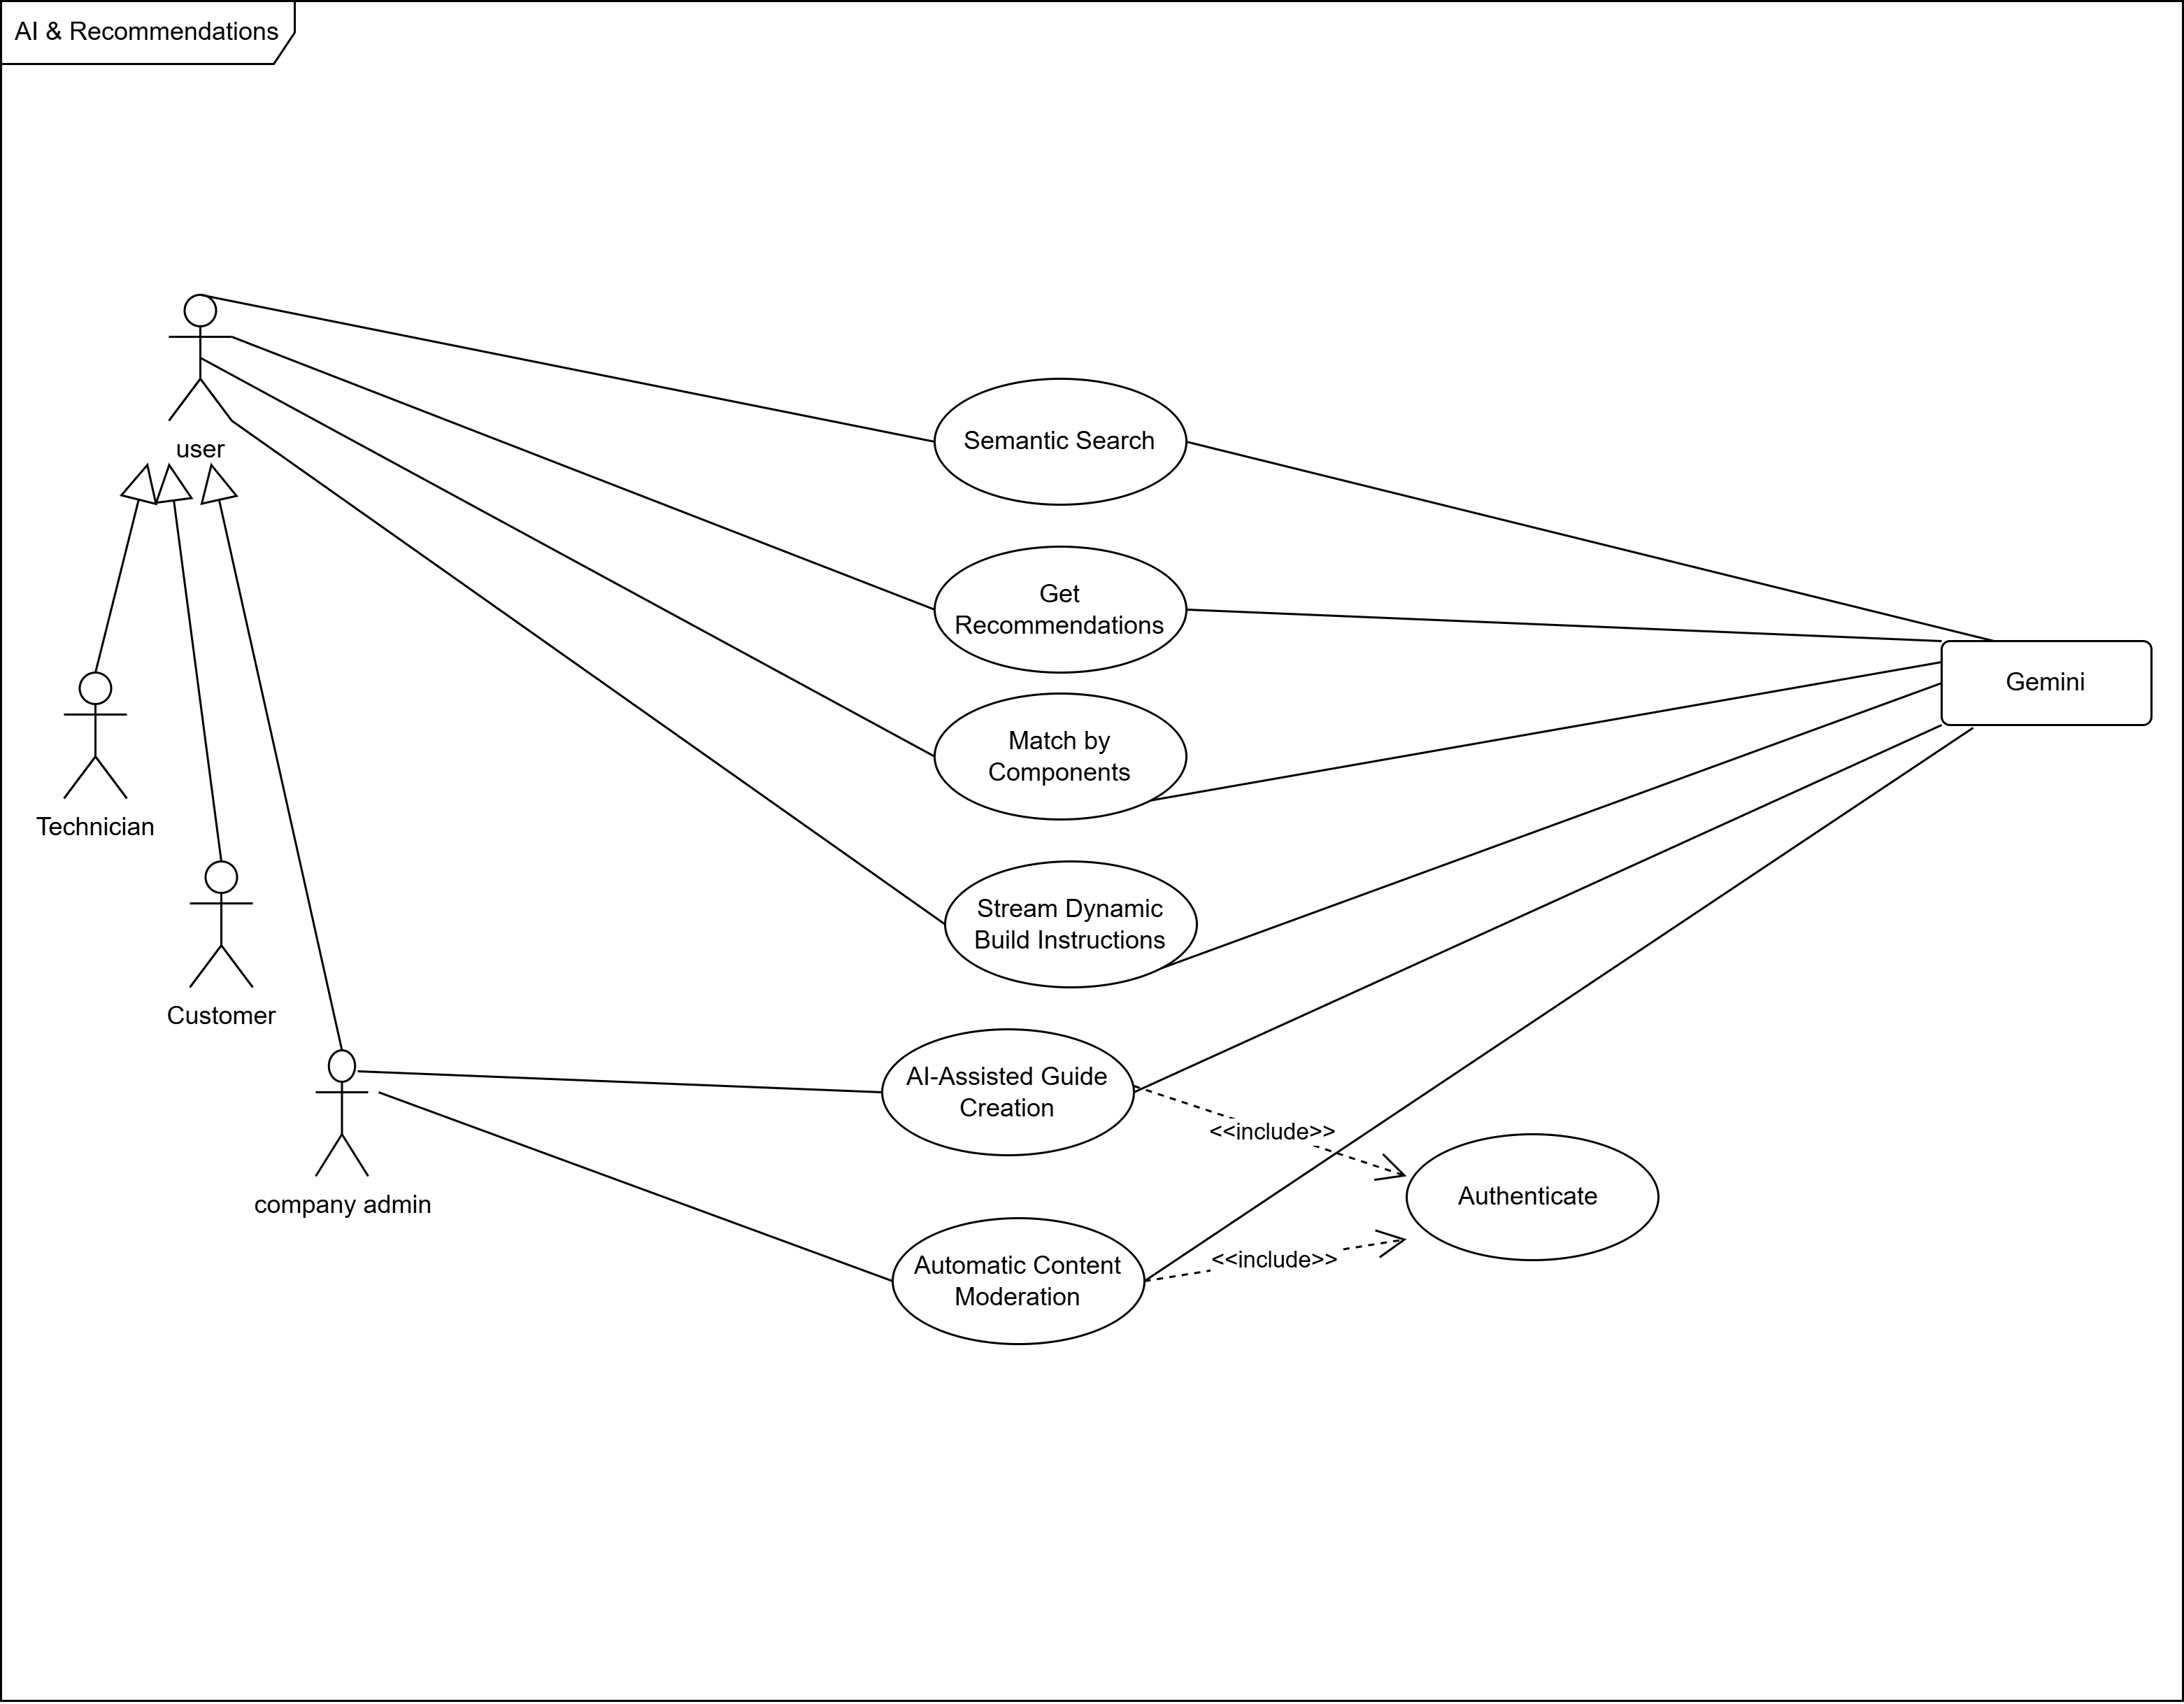
\includegraphics[width=0.95\textwidth]{images/usecase11.drawio.png}
\caption{Use case diagram -- Sprint 4: Hybrid Intelligence}
\label{fig:usecase_sprint4}
\end{figure}

\subsubsection{Use Case Refinement: Generate Recommendations}

The recommendation engine suggests alternative hardware models. Table~\ref{tab:generate_recs_desc} details this scenario.

\begin{table}[!htbp]
\centering
\caption{Textual description of the Generate Recommendations use case}
\label{tab:generate_recs_desc}
\begin{tabular}{lp{10cm}}
\toprule
\textbf{Element} & \textbf{Description} \\
\midrule
Use Case & Generate Recommendations \\
Actor & Client / Technician / Admin \\
Precondition & Client opens hardware details view. \\
Postcondition & Related models are listed based on similarity score. \\
Nominal Scenario &
1. User opens a product's main view. \newline
2. Frontend queries backend matching-endpoint with product ID. \newline
3. Backend runs vector semantic lookup on product embeddings. \newline
4. App lists high-scoring recommendations in a grid. \\
\bottomrule
\end{tabular}
\end{table}

\subsubsection{Use Case Refinement: Component-Based Recommendation}

This workflow matches physical components to compatible equipment. Table~\ref{tab:comp_recs_desc} outlines the steps.

\begin{table}[!htbp]
\centering
\caption{Textual description of the Component-Based Recommendation use case}
\label{tab:comp_recs_desc}
\begin{tabular}{lp{10cm}}
\toprule
\textbf{Element} & \textbf{Description} \\
\midrule
Use Case & Component-Based Recommendation \\
Actor & Client \\
Precondition & Client opens parts picker page. \\
Postcondition & Matching products render in a list. \\
Nominal Scenario &
1. Client clicks component check-boxes in side menu. \newline
2. Client clicks search matches. \newline
3. Backend calculates compatibility scores using ComponentMatchingService. \newline
4. App lists matching products in results page. \\
\bottomrule
\end{tabular}
\end{table}

\subsubsection{Use Case Refinement: Intelligent Search}

Intelligent search parses natural language questions. Table~\ref{tab:intel_search_desc} defines the conditions.

\begin{table}[!htbp]
\centering
\caption{Textual description of the Intelligent Search use case}
\label{tab:intel_search_desc}
\begin{tabular}{lp{10cm}}
\toprule
\textbf{Element} & \textbf{Description} \\
\midrule
Use Case & Intelligent Search \\
Actor & Client / Technician / Admin \\
Precondition & User is on search input field. \\
Postcondition & Ranked search results show up on search page. \\
Nominal Scenario &
1. User types a question like 'how to fix screen'. \newline
2. Backend dispatches text string to Gemini API for embedding. \newline
3. Server runs vector similarity query on MongoDB collection. \newline
4. Frontend renders ranked matches sorted by cosine score. \\
\bottomrule
\end{tabular}
\end{table}

\subsubsection{Use Case Refinement: Generate AI Build Instructions}

Technical editors generate draft manuals using the AI pipeline. Table~\ref{tab:ai_build_desc} maps the steps.

\begin{table}[!htbp]
\centering
\caption{Textual description of the Generate AI Build Instructions use case}
\label{tab:ai_build_desc}
\begin{tabular}{lp{10cm}}
\toprule
\textbf{Element} & \textbf{Description} \\
\midrule
Use Case & Generate AI Build Instructions \\
Actor & Company Admin / Technician \\
Precondition & Product model is mapped to parts in DB. \\
Postcondition & AI-drafted manual is loaded as a starting draft. \\
Nominal Scenario &
1. Writer picks product model. \newline
2. Writer clicks draft manual. \newline
3. Backend sends prompt containing components metadata to Gemini API. \newline
4. Editor page loads generated markdown text. \\
\bottomrule
\end{tabular}
\end{table}

\subsection{Sequence Diagrams}

Figure~\ref{fig:seq_sprint4} tracks the dynamic message sequence during parts recommendation and AI build generation.

\begin{figure}[!htbp]
\centering
\resizebox{\textwidth}{!}{%
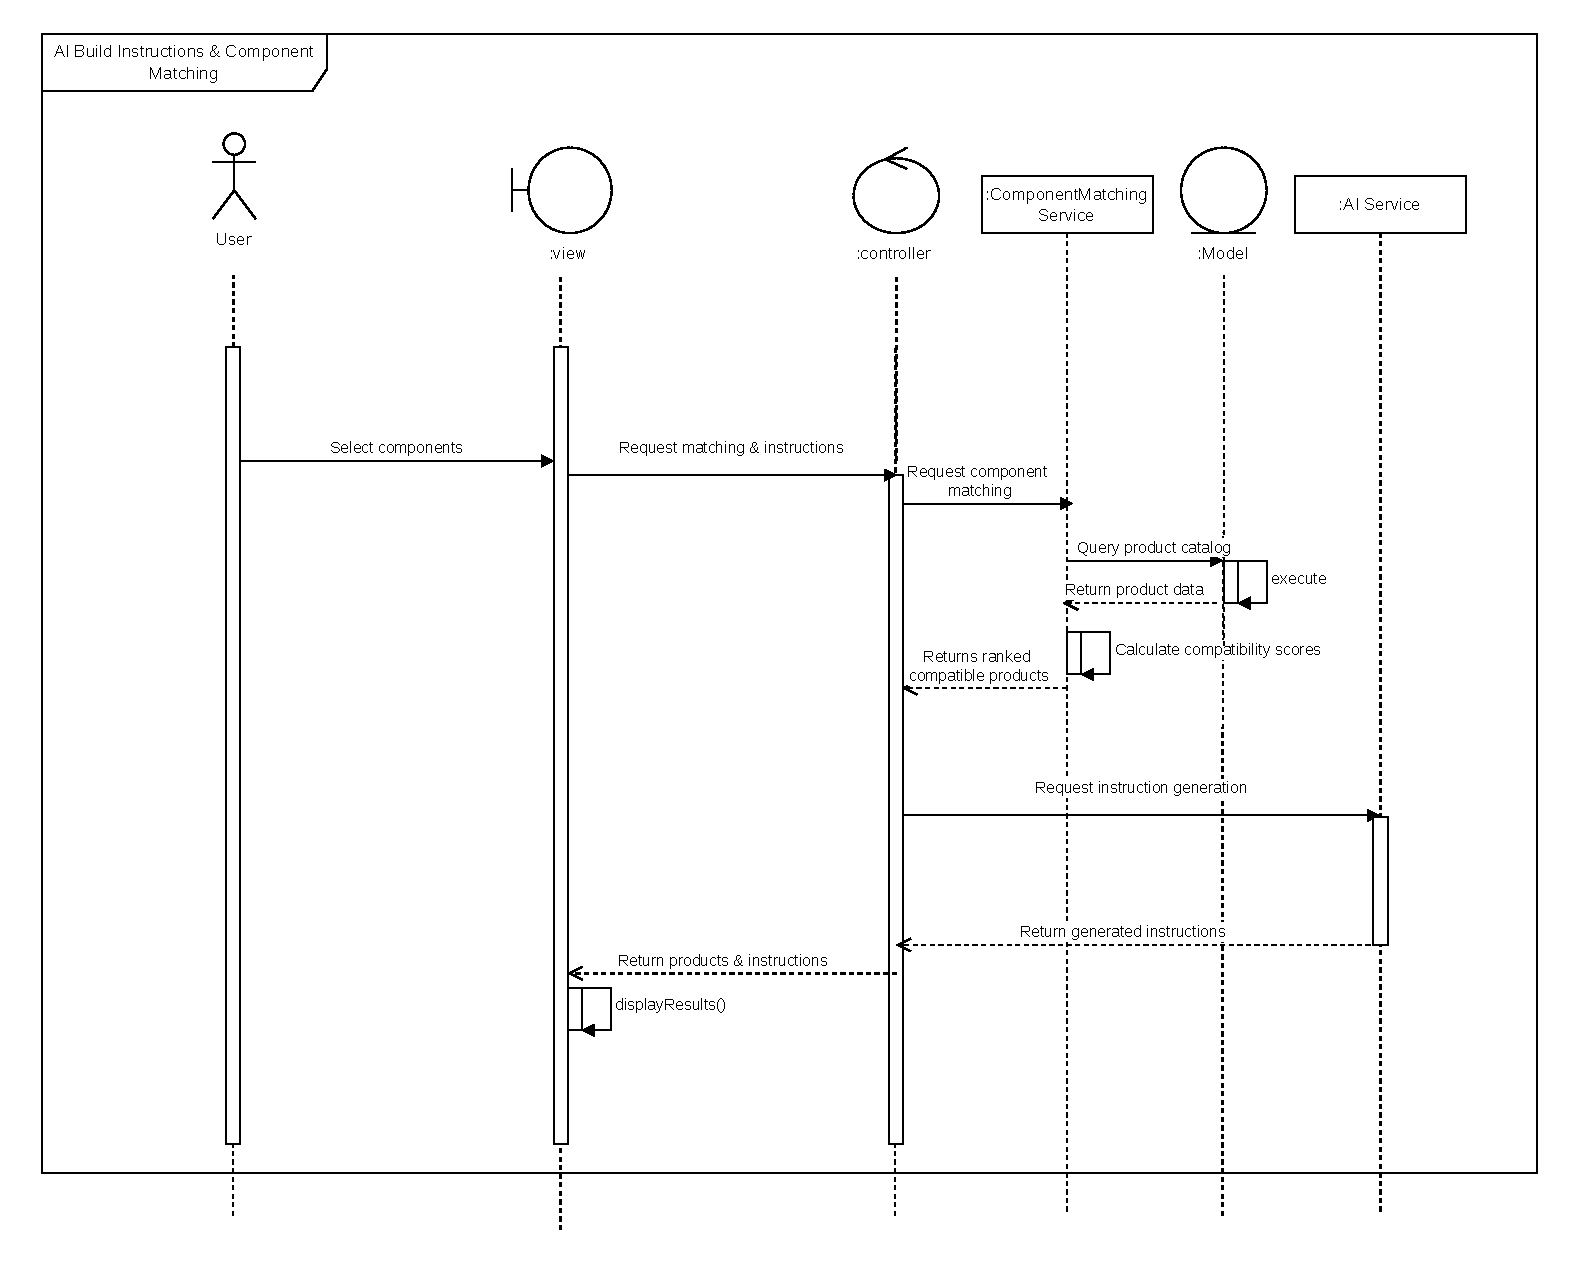
\includegraphics[width=0.95\textwidth]{images/seq7_ai_build.pdf}%
}
\caption{Sequence diagram: Component recommendation and instruction process}
\label{fig:seq_sprint4}
\end{figure}

\subsection{User Interfaces Overview}

Figure~\ref{fig:web_recs} and Figure~\ref{fig:mobile_recs} illustrate the search and recommendation layouts we implemented for web and mobile.

\begin{figure}[!htbp]
 \centering
 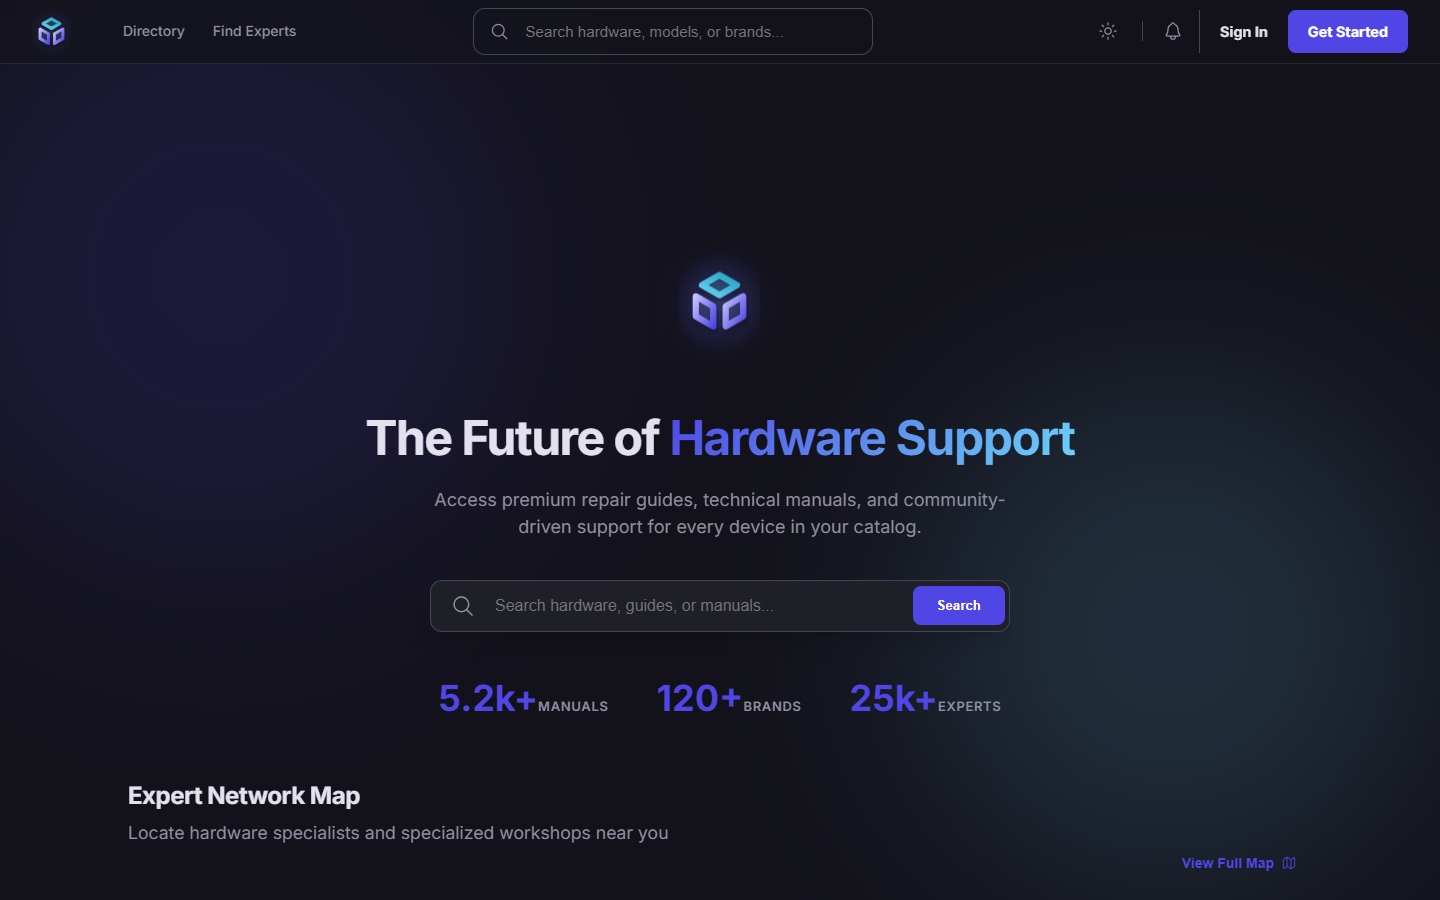
\includegraphics[width=0.45\textwidth]{images/web_recommendations.png}
 \hfill
 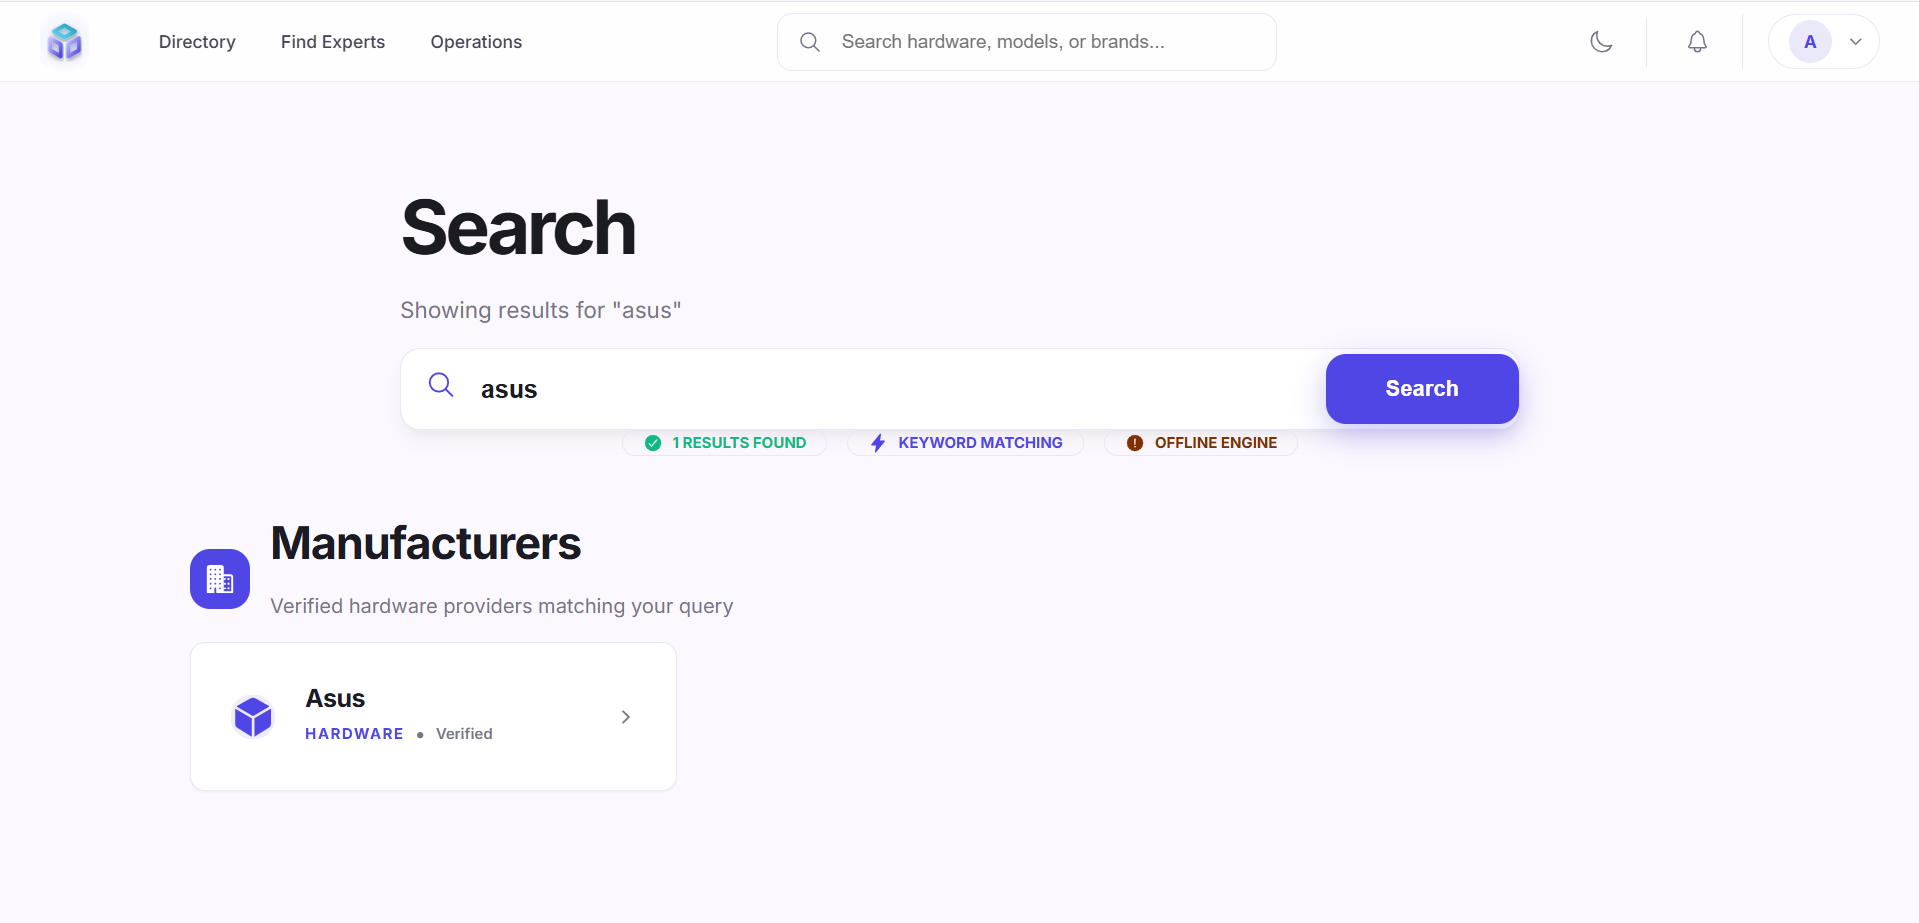
\includegraphics[width=0.45\textwidth]{images/search engine.PNG}
 \caption{Web interfaces -- Semantic search and recommendations}
 \label{fig:web_recs}
 \end{figure}

\begin{figure}[!htbp]
\centering
\includegraphics[width=0.4\textwidth]{images/mobile_recommendations.png}
\caption{Mobile interface – Recommendation system}
\label{fig:mobile_recs}
\end{figure}

\subsection{Technical Challenges and Solutions}

Integrating external AI services introduced two main challenges:
\begin{itemize}
    \item \textbf{API Rate Limits}: The Google Gemini API restricts query rates. We solved this by implementing an in-memory queue with exponential backoff on retries.
    \item \textbf{Token Limits}: Long manuals consume context windows. We resolved this by pre-segmenting guides into text chunks of maximum 1000 characters before embedding.
\end{itemize}

\section{Conclusion}

In Release 4, we finished implementing the hybrid intelligence layer. Combining Google Gemini embeddings with deterministic schema validations gave us a highly accurate recommendation engine and semantic search. In the next chapter, we look at Release 5, which completes the system lifecycle by adding support ticketing and coordinating repair technicians.

\chapter{Release 5 : Maintenance Requests \& Technician Workflow}

\section{Introduction}

This chapter outlines the development of the support request pipeline and verified technician workspace. Release 5 completes the platform lifecycle, letting clients submit tickets when manual steps fail, and providing a portal for technicians to manage jobs.

We focused on implementing four key features:
\begin{itemize}
    \item \textbf{Support Requests}: We designed a request intake form where clients describe issues, select urgency levels, and specify appliance models.
    \item \textbf{Technician Workspace}: We built a ticket pool where approved technicians search for, claim, and update active repair requests.
    \item \textbf{Technician Onboarding}: We built a verification dashboard where super administrators review uploaded certifications and proof of expertise.
    \item \textbf{State-Transition Validation}: We implemented backend state validation rules to ensure tickets transition correctly from pending, to claimed, and finally to resolved.
\end{itemize}

\section{Sprint Backlog -- Maintenance \& Technician}

Table~\ref{tab:sprint5_backlog} details the final sprint backlog tasks, including their priority and scope.

\renewcommand{\arraystretch}{1.3}
\setlength{\tabcolsep}{8pt}

\begin{table}[!htbp]
\centering
\caption{User stories for Release 5 (Maintenance \& Technician)}
\label{tab:sprint5_backlog}
\resizebox{\textwidth}{!}{%
\begin{tabular}{clp{8cm}c}
\toprule
\textbf{ID} & \textbf{Feature / Epic} & \textbf{Description} & \textbf{Priority} \\
\midrule
16 & Technician Profile & Certification submission, profile reviews, and administrator verification. & High \\
17 & Maintenance Tickets & Creation, status monitoring, and transition rules for repair requests. & Medium \\
\bottomrule
\end{tabular}%
}
\end{table}

\section{Refinement of Use Cases}

To structure our ticketing database collections and restrict actions by role, we refined three use cases detailing the request and approval workflows.

\subsection{Sprint 5 Use Case Diagrams and Textual Descriptions}

\subsubsection{Use Case Refinement: Submit Maintenance Request}

Clients file a ticket if they cannot fix an issue using the online manuals. Figure~\ref{fig:usecase_submit_maintenance} and Table~\ref{tab:submit_maintenance_desc} show how tickets are submitted and saved.

\begin{figure}[H]
\centering
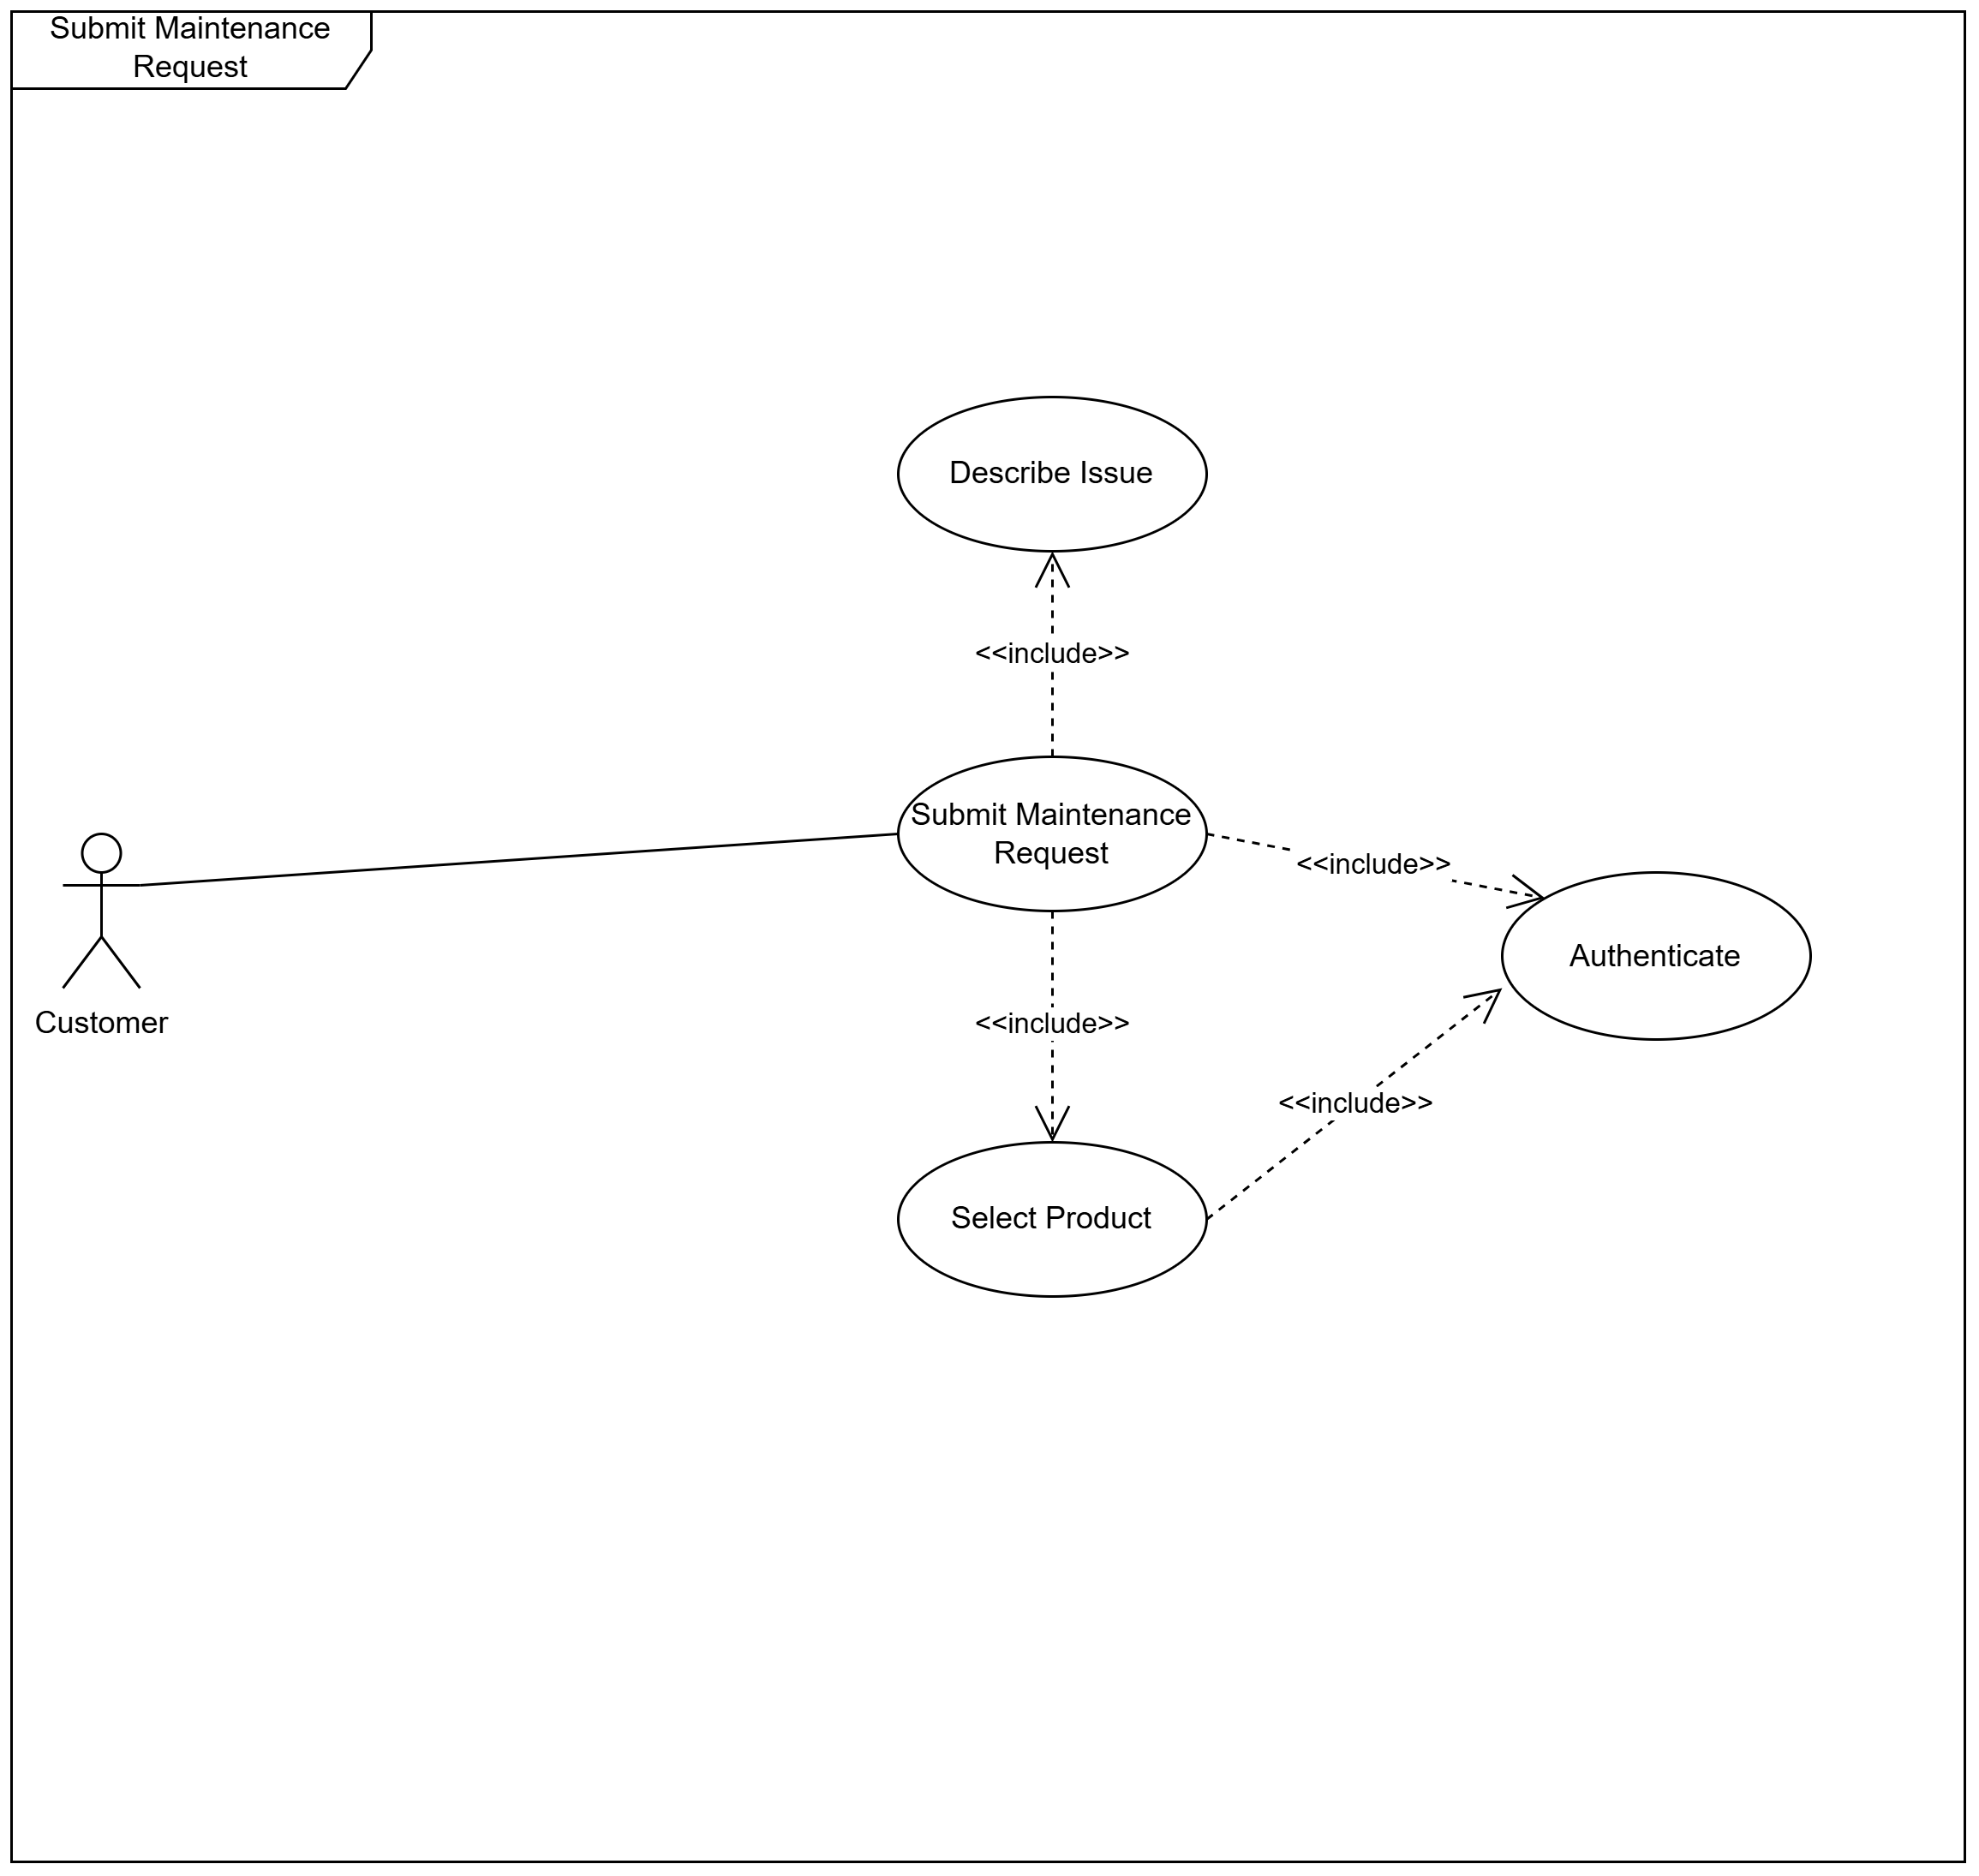
\includegraphics[width=0.8\textwidth]{images/usecase14.drawio.png}
\caption{Use case diagram: Submit maintenance request}
\label{fig:usecase_submit_maintenance}
\end{figure}

\begin{table}[H]
\centering
\caption{Textual description of the Submit Maintenance Request use case}
\label{tab:submit_maintenance_desc}
\begin{tabular}{lp{10cm}}
\toprule
\textbf{Element} & \textbf{Description} \\
\midrule
Use Case & Submit Maintenance Request \\
Actor & Client (Customer) \\
Precondition & User is logged in and opens the help desk tab. \\
Postcondition & System creates a ticket with status 'pending' in MongoDB. \\
Nominal Scenario &
1. Client opens the support request form. \newline
2. Client fills in issue details, selects urgency, and enters the model. \newline
3. Backend validates input payload. \newline
4. Database creates a 'pending' ticket linked to the client's account. \\
\bottomrule
\end{tabular}
\end{table}

\subsubsection{Use Case Refinement: Follow and Manage Maintenance Requests}

Approved technicians claim and update tickets via their mobile workspace. Figure~\ref{fig:usecase_manage_maintenance} and Table~\ref{tab:manage_maintenance_desc} illustrate the ticket lifecycle rules.

\begin{figure}[H]
\centering
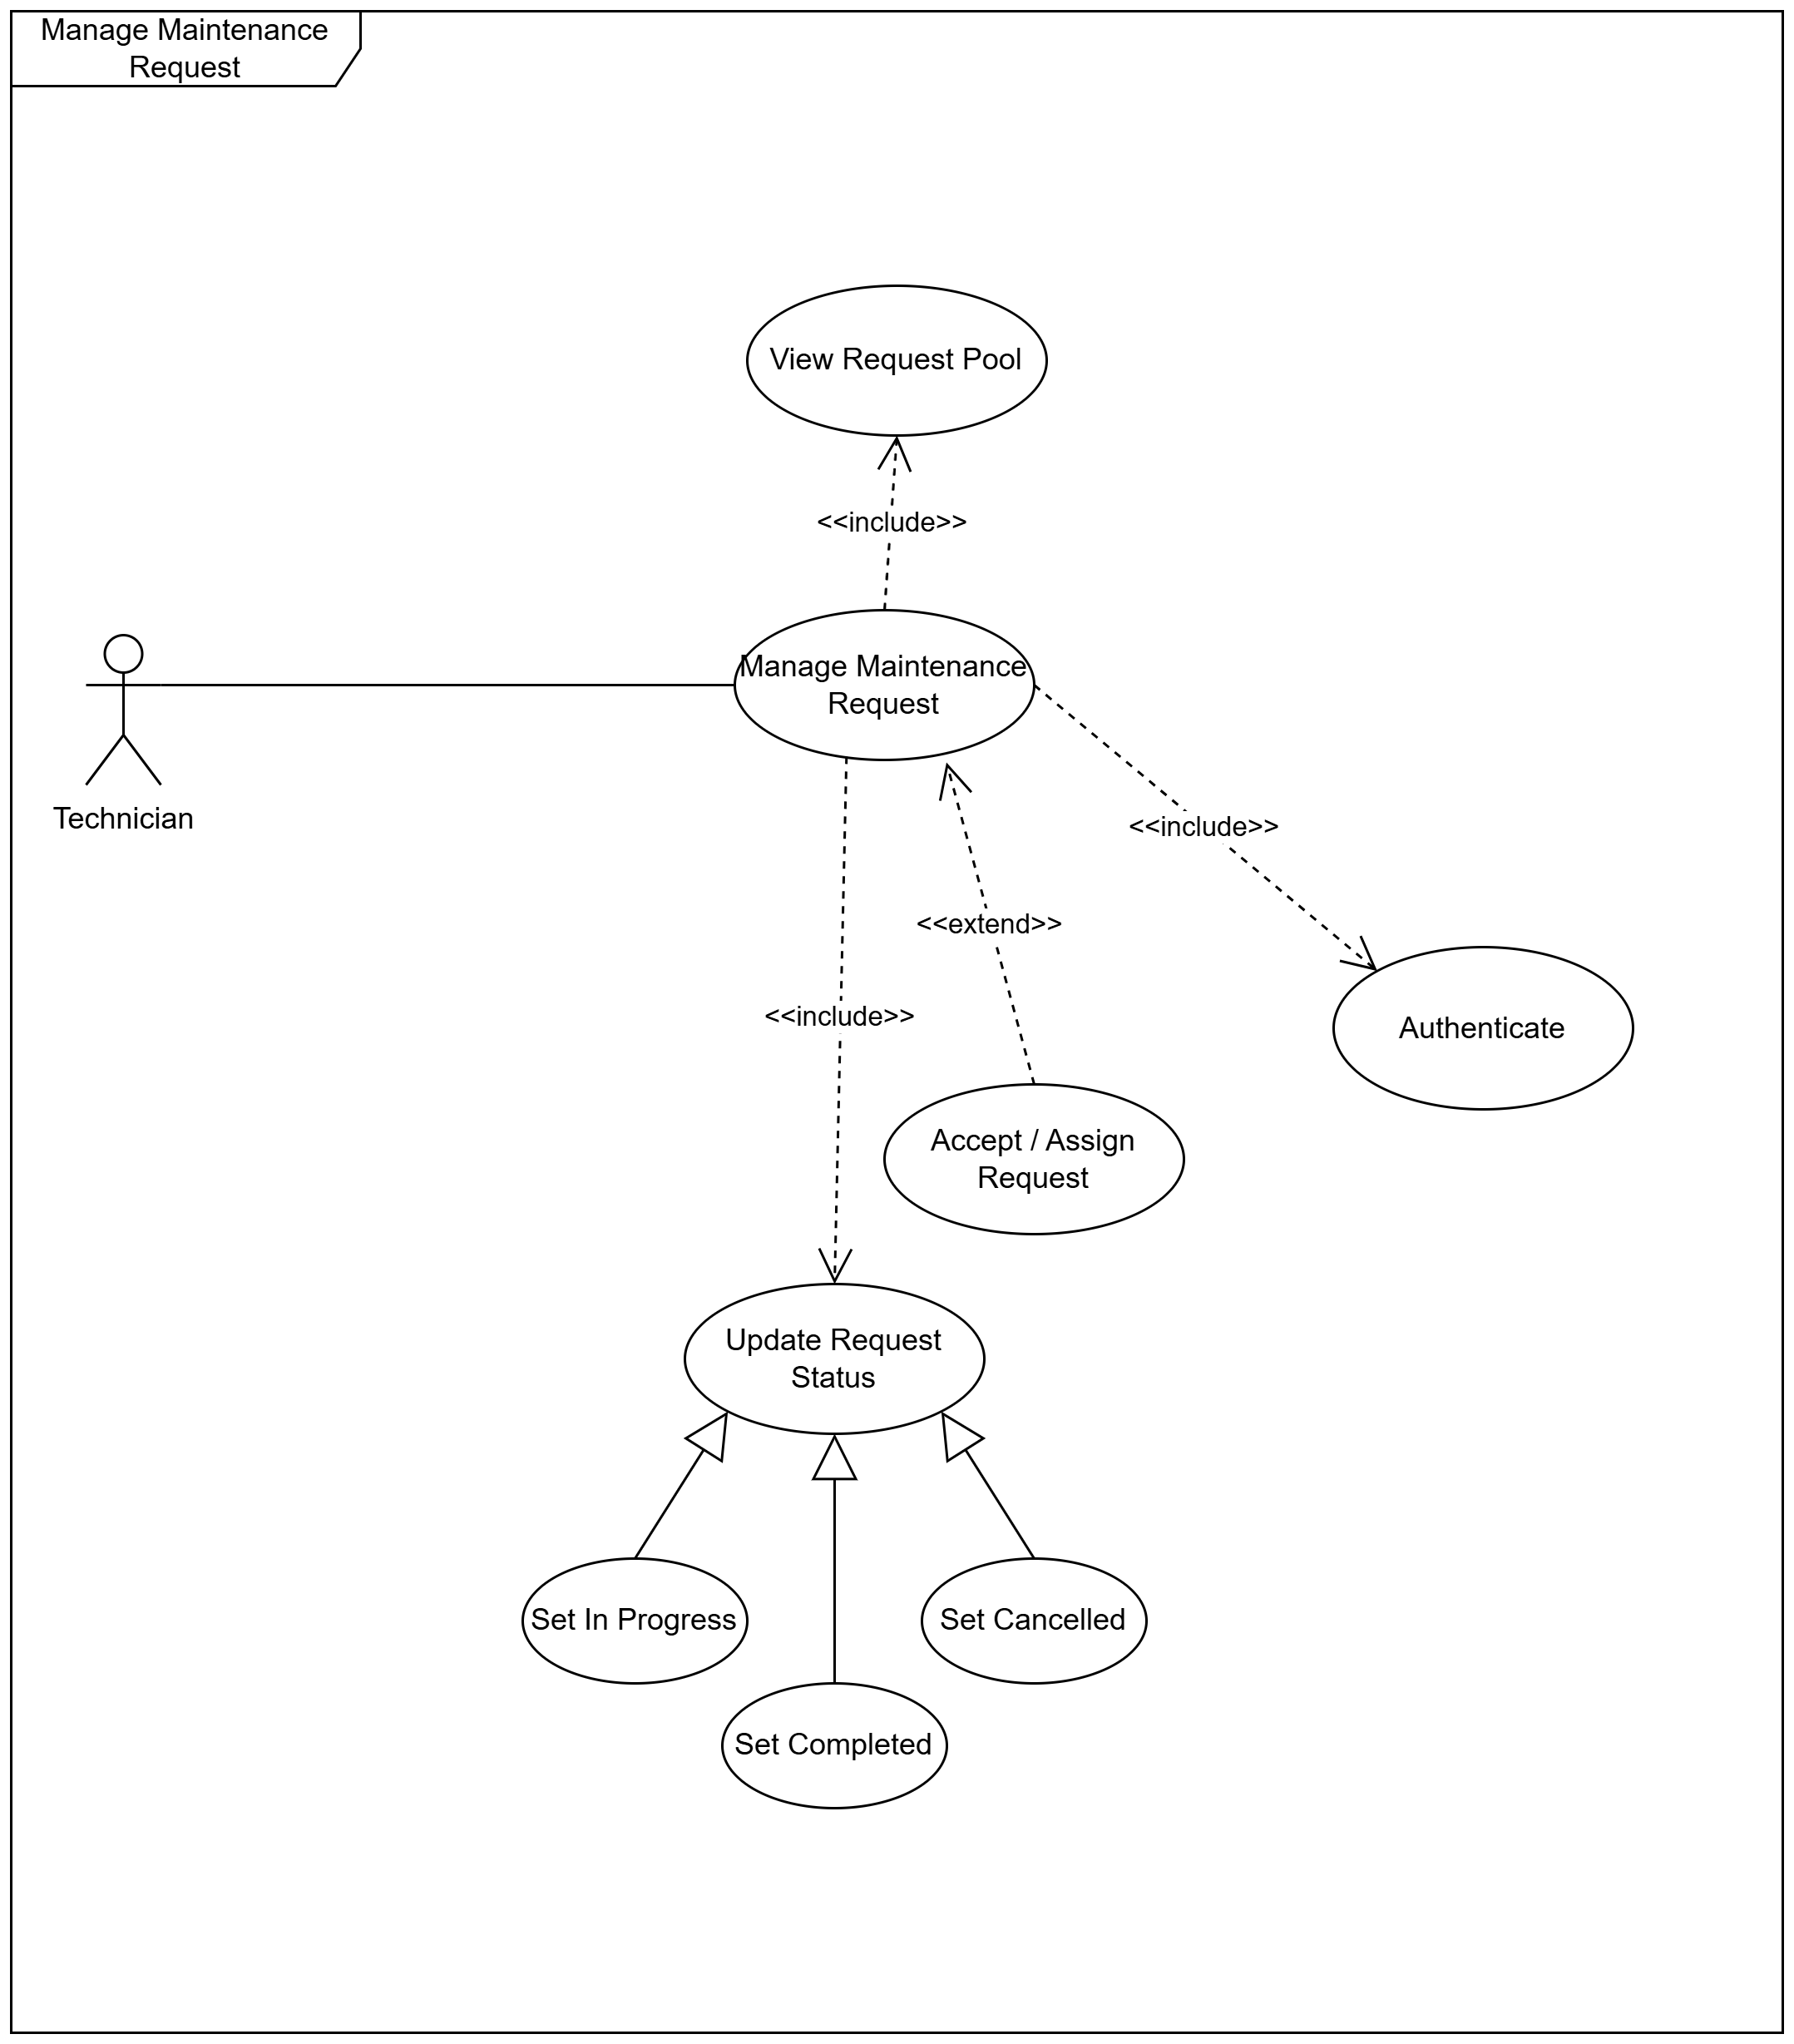
\includegraphics[width=0.75\textwidth]{images/usecase12.drawio.png}
\caption{Use case diagram: Follow and manage maintenance requests}
\label{fig:usecase_manage_maintenance}
\end{figure}

\begin{table}[H]
\centering
\caption{Textual description of the Follow and Manage Maintenance Requests use case}
\label{tab:manage_maintenance_desc}
\begin{tabular}{lp{10cm}}
\toprule
\textbf{Element} & \textbf{Description} \\
\midrule
Use Case & Follow and Manage Maintenance Requests \\
Actor & Technician \\
Precondition & Technician is logged in with an active, approved profile. \\
Postcondition & System updates the ticket status to assigned, claimed, or resolved. \\
Nominal Scenario &
1. Technician opens the job board page. \newline
2. Backend filters and lists unclaimed tickets matching their category. \newline
3. Technician claims a ticket or updates its progress status. \newline
4. Backend validates transition rules and saves updates in MongoDB. \\
\bottomrule
\end{tabular}
\end{table}


\subsubsection{Use Case Refinement: Approve Technician Profile}

To ensure service quality, super administrators review and validate technician credentials. Figure~\ref{fig:usecase_approve_technician} and Table~\ref{tab:approve_technician_desc} detail this verification pipeline.

\begin{figure}[H]
\centering
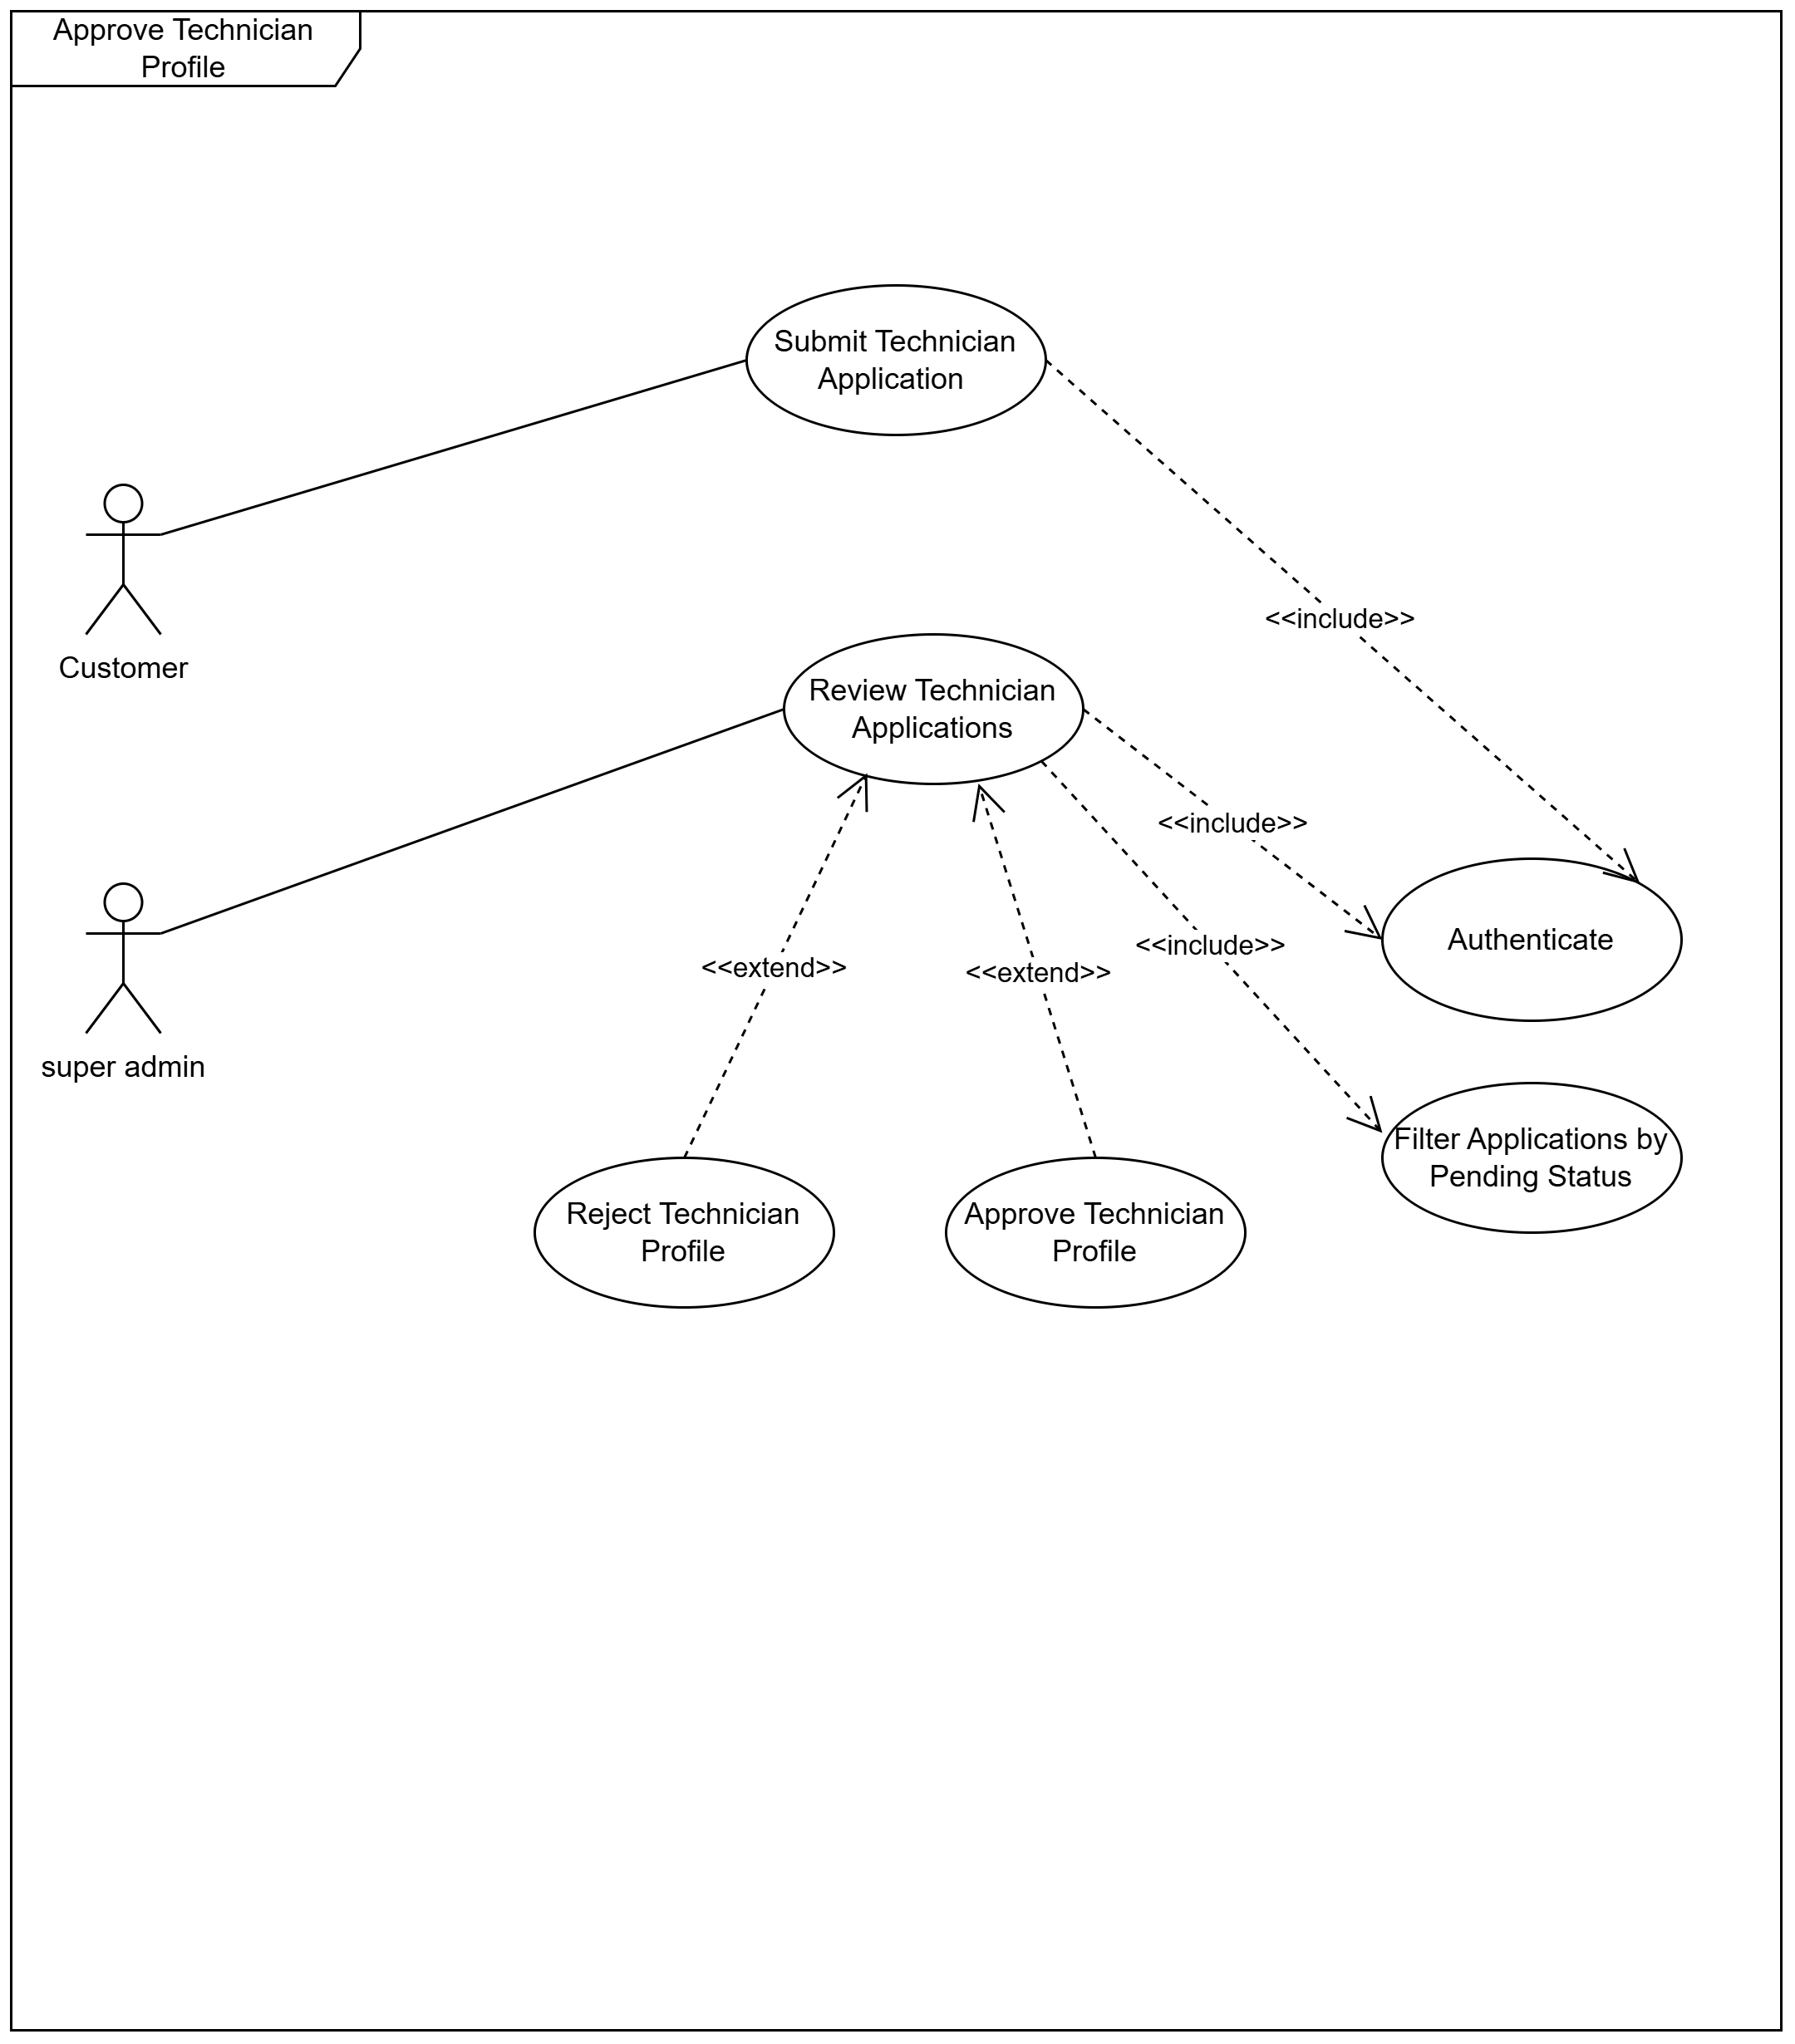
\includegraphics[width=0.8\textwidth]{images/usecase13.drawio.png}
\caption{Use case diagram: Approve Technician Profile}
\label{fig:usecase_approve_technician}
\end{figure}

\begin{table}[H]
\centering
\caption{Textual description of the Approve Technician Profile use case}
\label{tab:approve_technician_desc}
\begin{tabular}{lp{10cm}}
\toprule
\textbf{Element} & \textbf{Description} \\
\midrule
Use Case & Approve Technician Profile \\
Actor & Super Admin, Technician Applicant (Customer) \\
Precondition & A technician applicant uploads qualifications and profile data. \\
Postcondition & Admin approves the applicant, unlocking the technician dashboard. \\
Nominal Scenario &
1. Applicant uploads professional documents to their profile page. \newline
2. Super Admin retrieves pending verification list. \newline
3. Super Admin reviews and validates uploaded documents. \newline
4. Backend updates user role to 'technician' and broadcasts a websocket alert. \\
\bottomrule
\end{tabular}
\end{table}

\subsection{Class Diagram}

The class diagram in Figure~\ref{fig:sprint5_class} shows the database relationships, connecting \texttt{Maintenance\-Request} to the reporting \texttt{User} and the assigned \texttt{Technician\-Profile}.

\begin{figure}[!htbp]
\centering
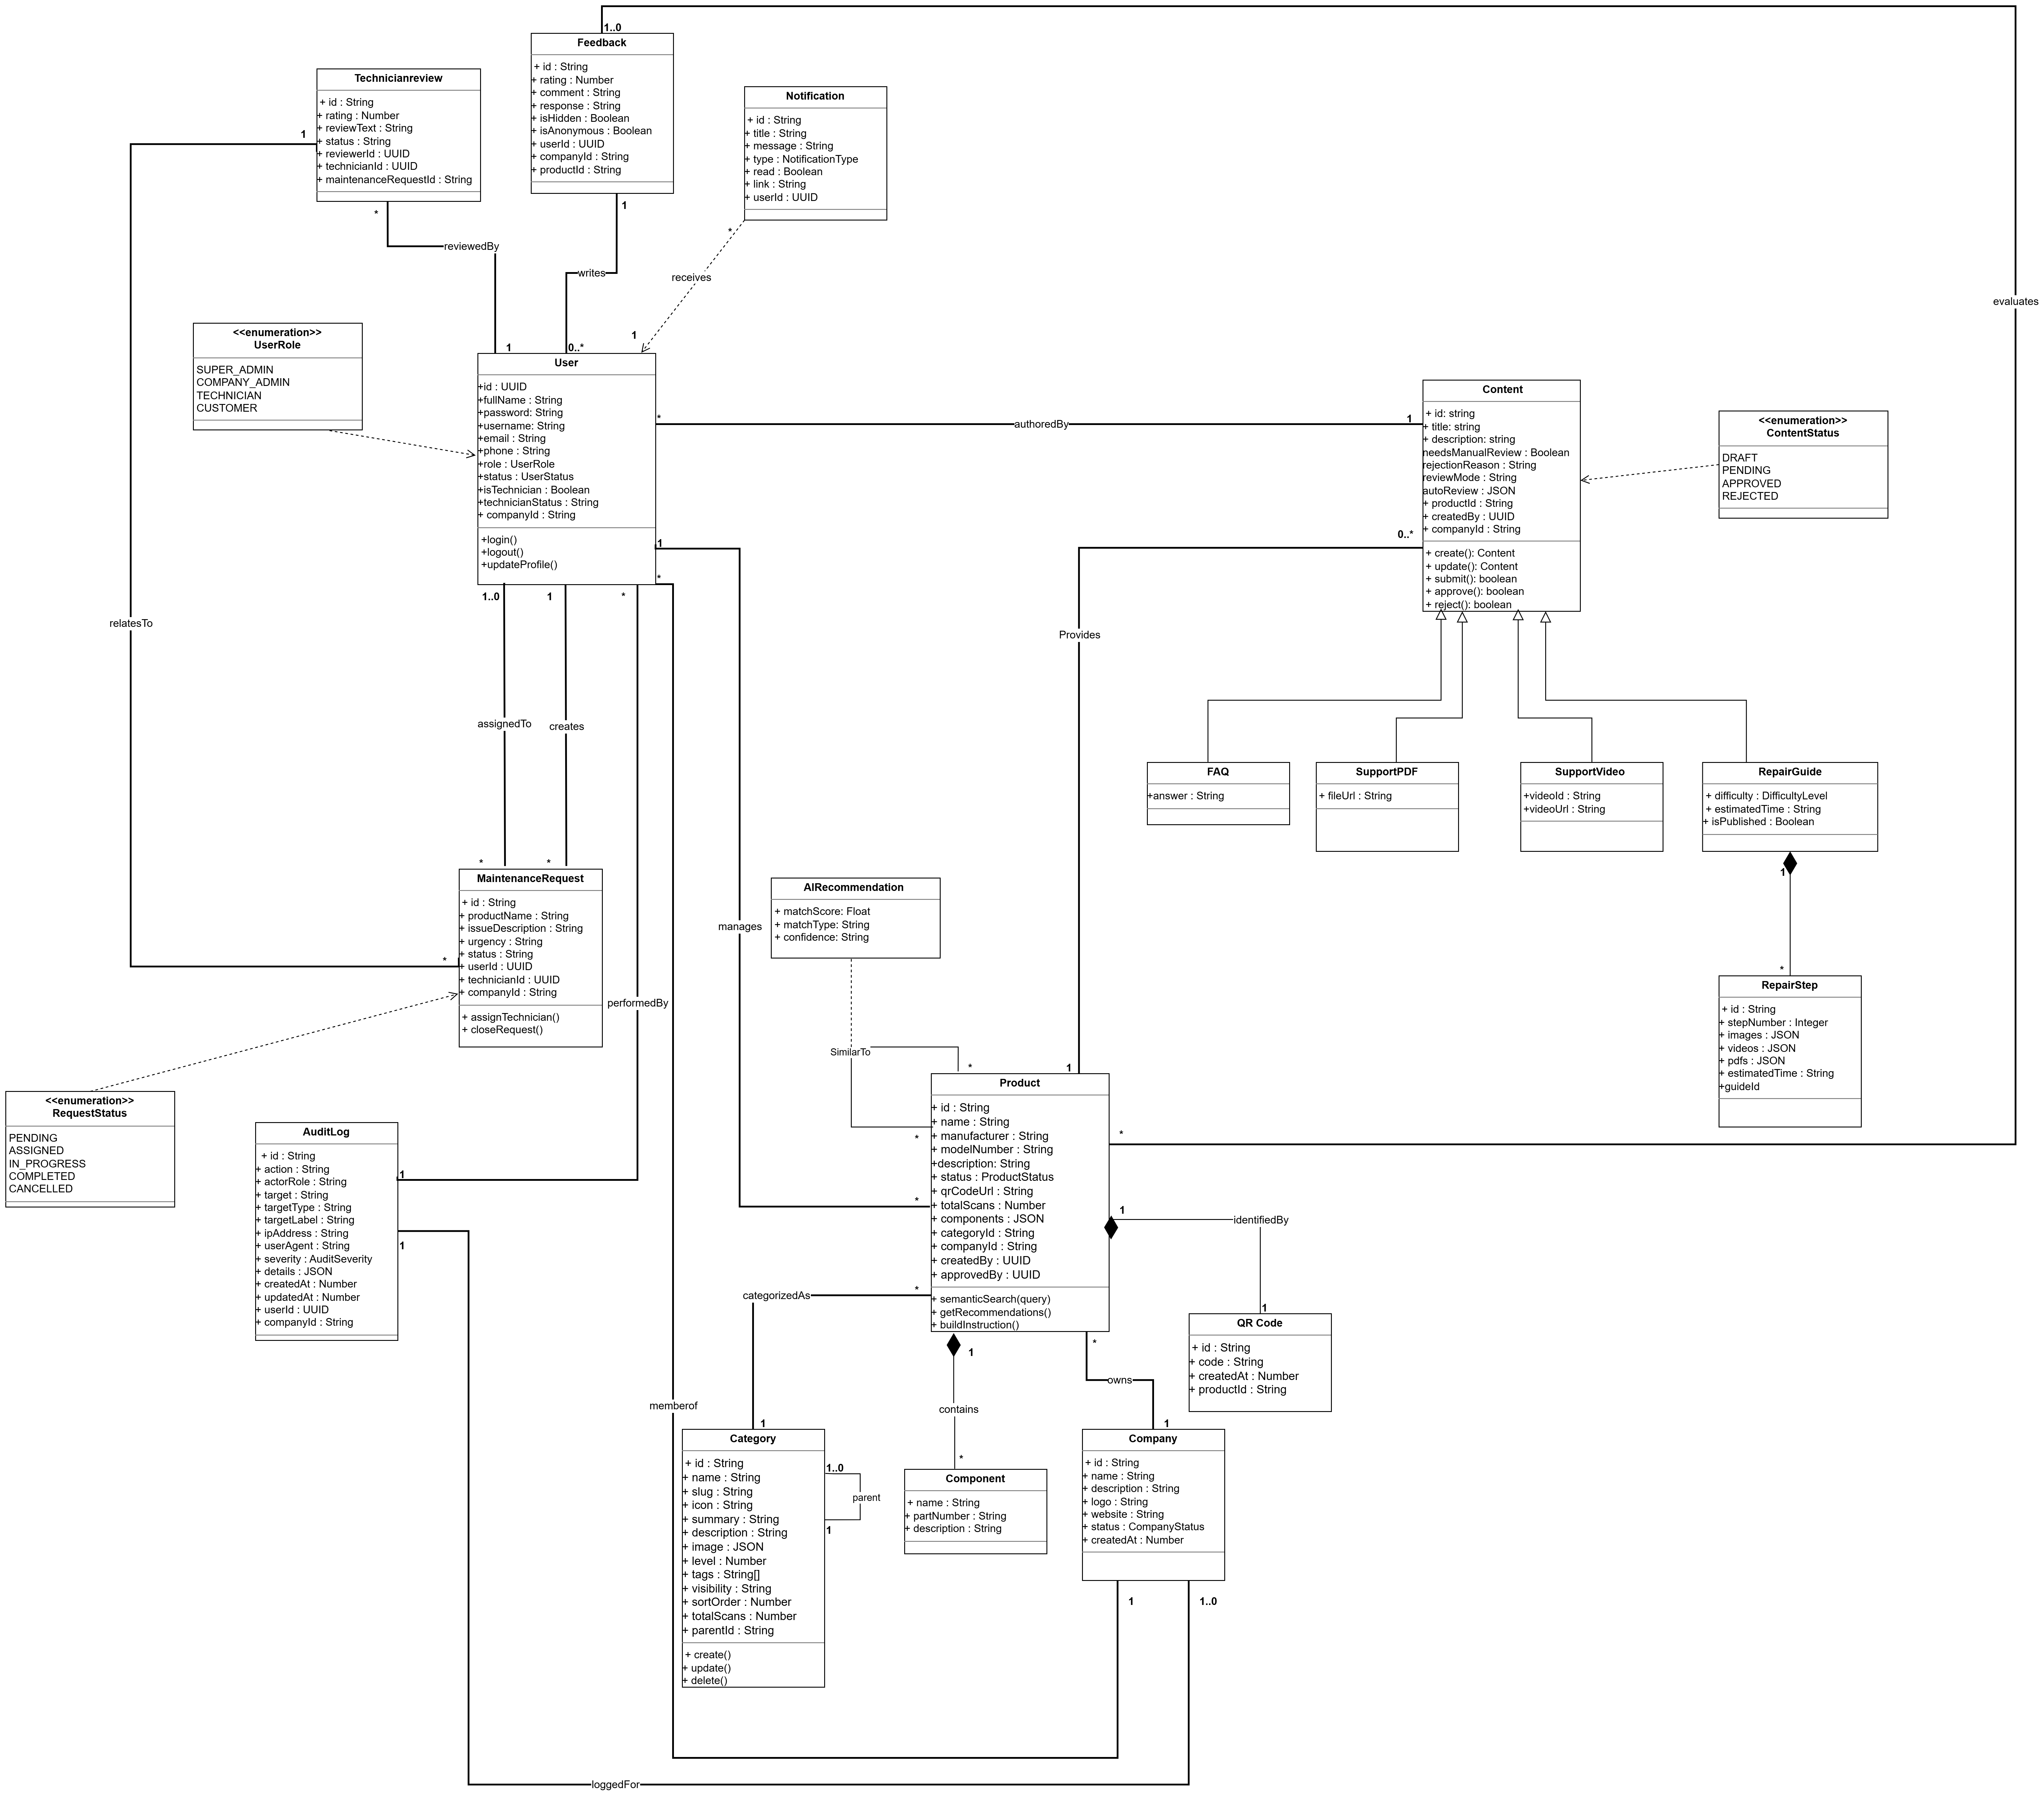
\includegraphics[width=0.9\textwidth]{images/sprint5class5.drawio.png}
\caption{Class diagram -- Maintenance requests and technician workflow}
\label{fig:sprint5_class}
\end{figure}

\subsection{Sequence Diagrams}

We mapped out the message exchange sequences to visualize how the system handles technician applications.

\subsubsection{Sequence Diagram: Become a Technician Application}

Figure~\ref{fig:seq_technician_app} details the sequence of API requests, document storage, and administrator review approvals.

\begin{figure}[!htbp]
\centering
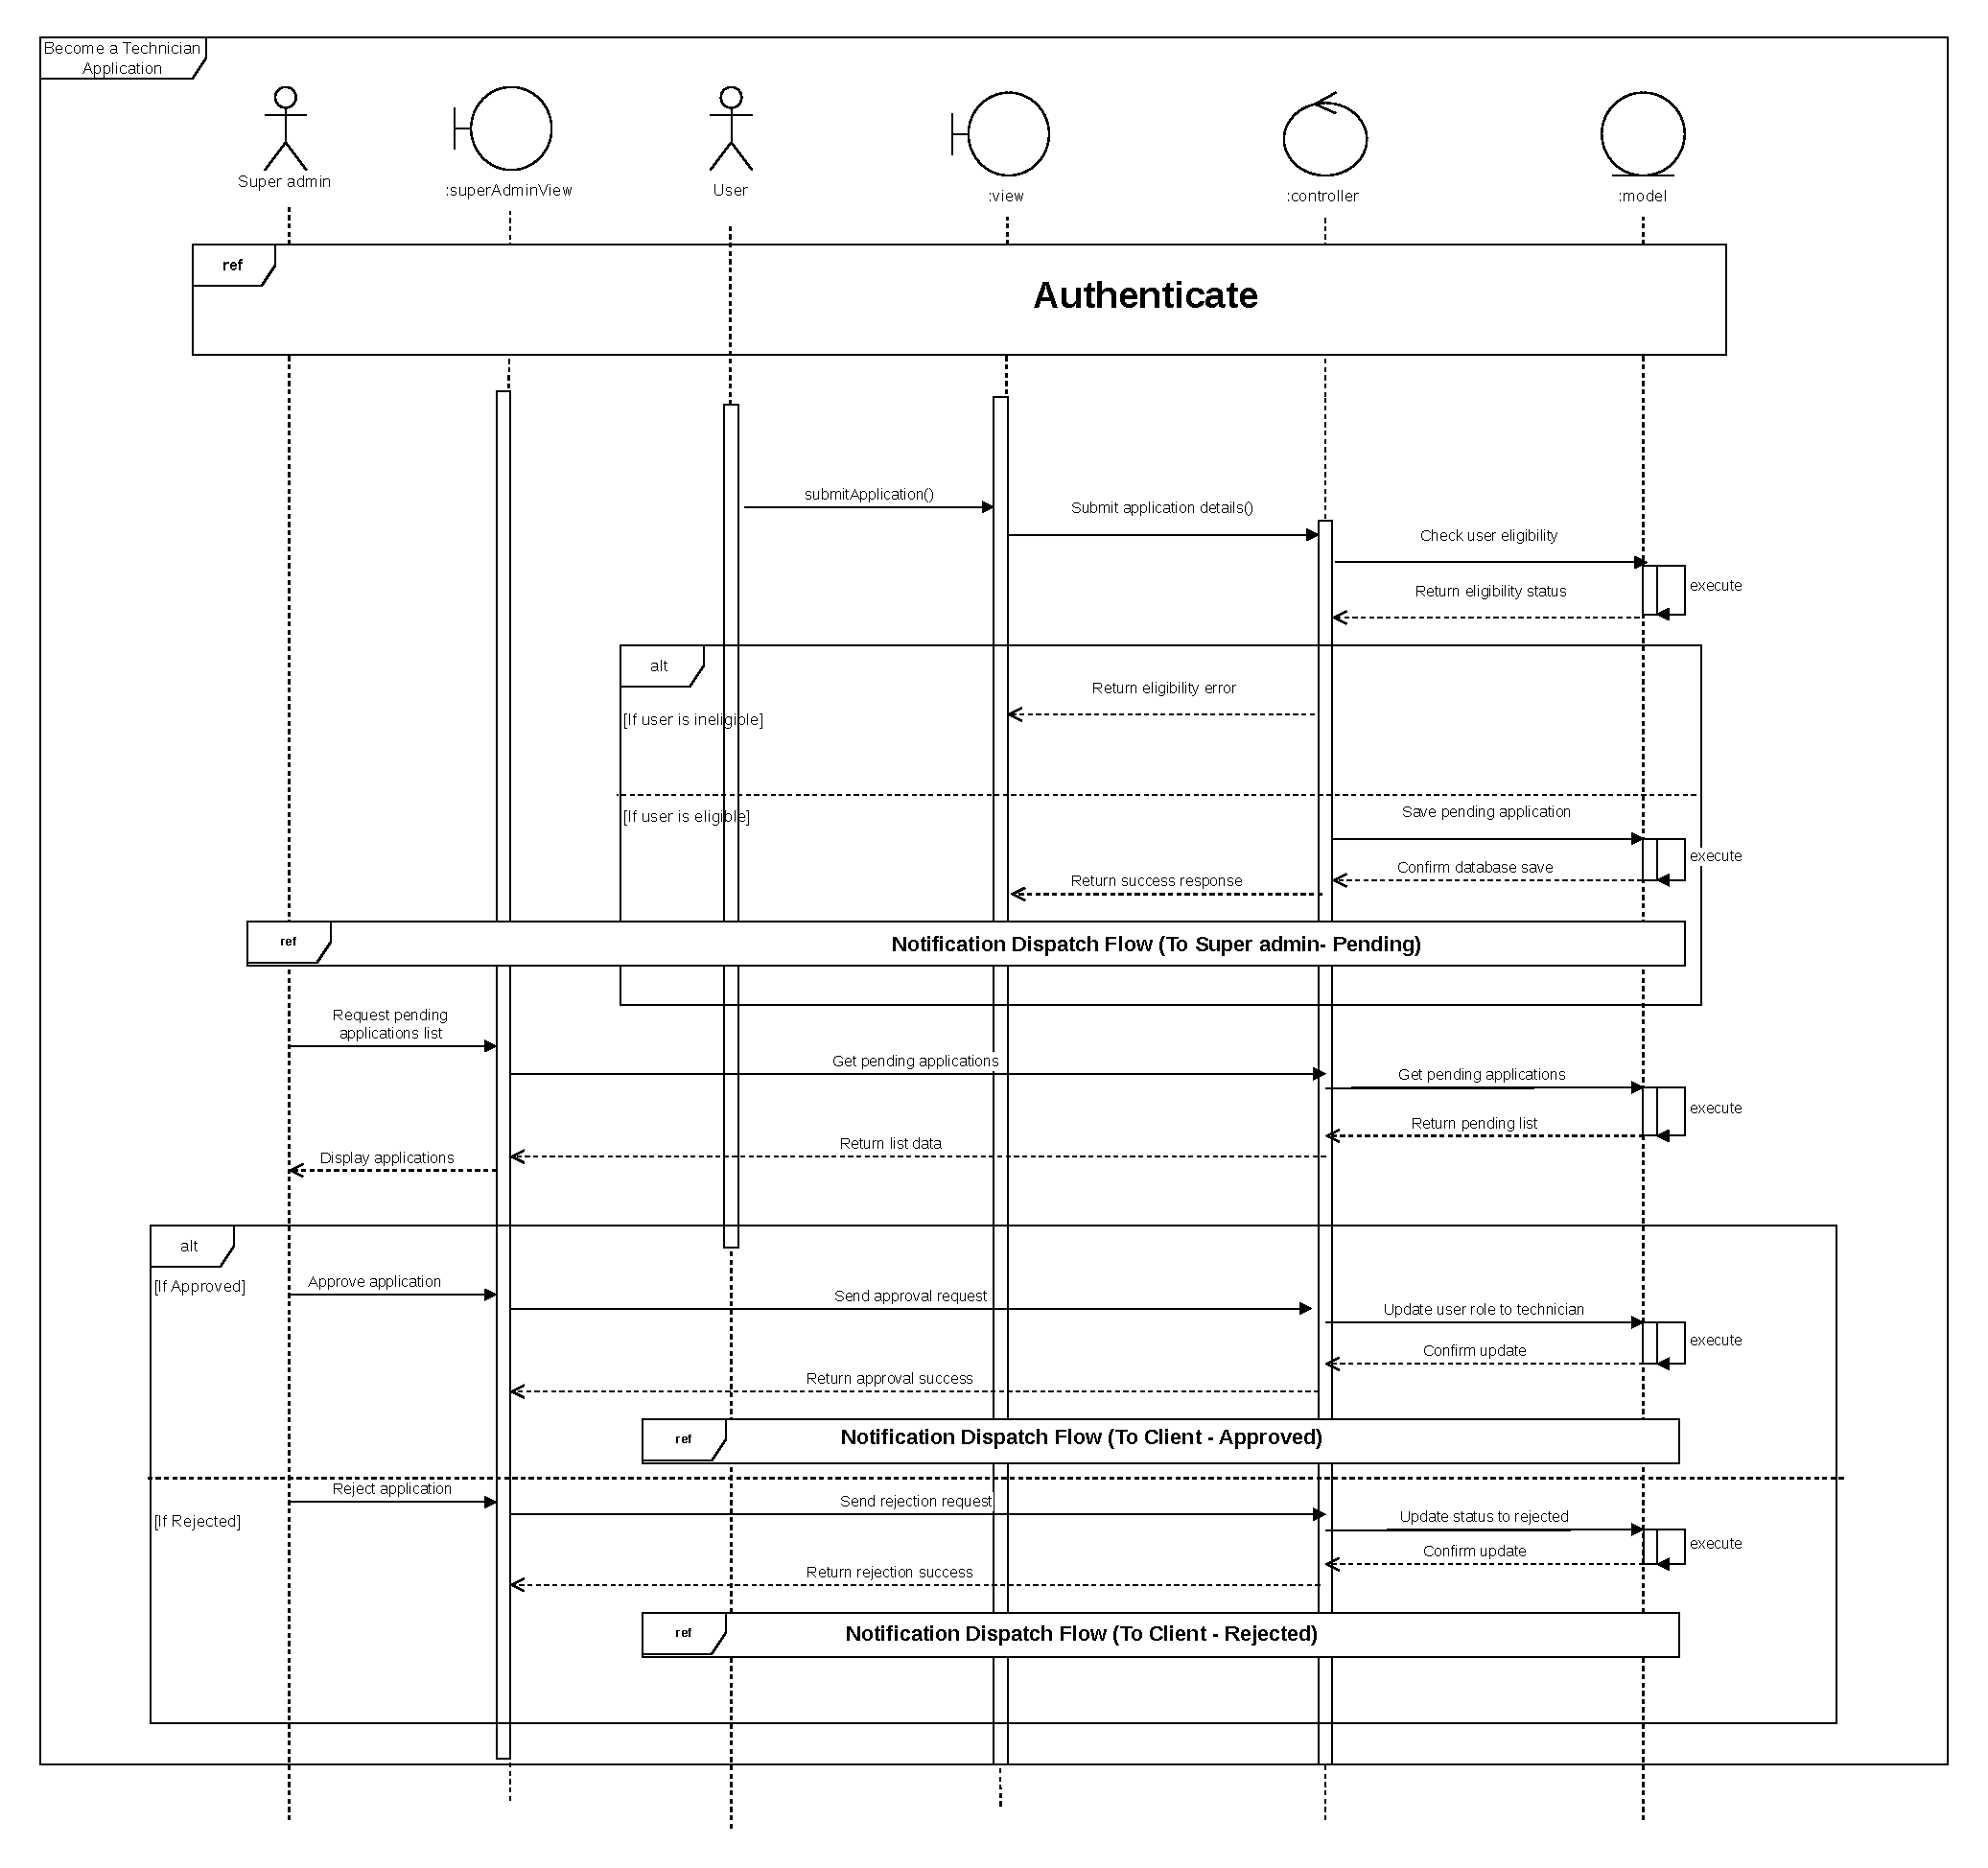
\includegraphics[width=0.9\textwidth]{images/seq9_technician.pdf}
\caption{Sequence diagram: Become a technician application}
\label{fig:seq_technician_app}
\end{figure}

\section{User Interface Overview}

\subsection{Web Interfaces}

The administration dashboards in Figure~\ref{fig:web_matching} show where admins manage technician requests and how technicians view their service job pools.

\begin{figure}[!htbp]
 \centering
 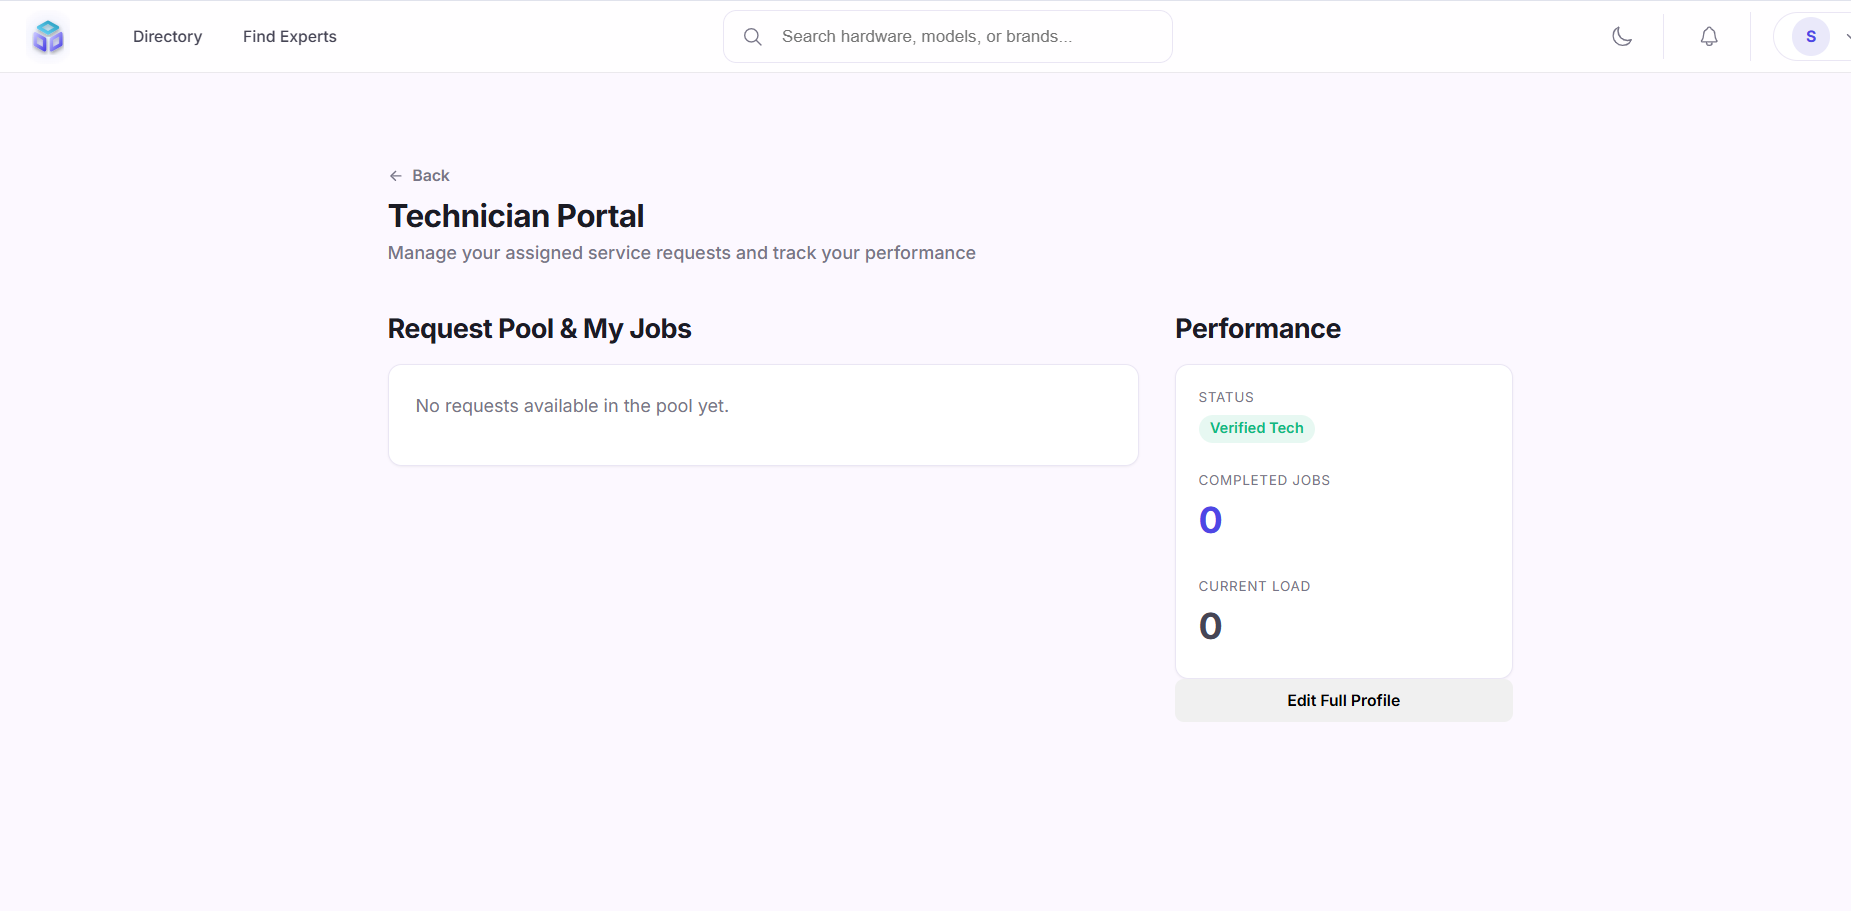
\includegraphics[width=0.48\textwidth]{images/technician request list.PNG}
 \hfill
 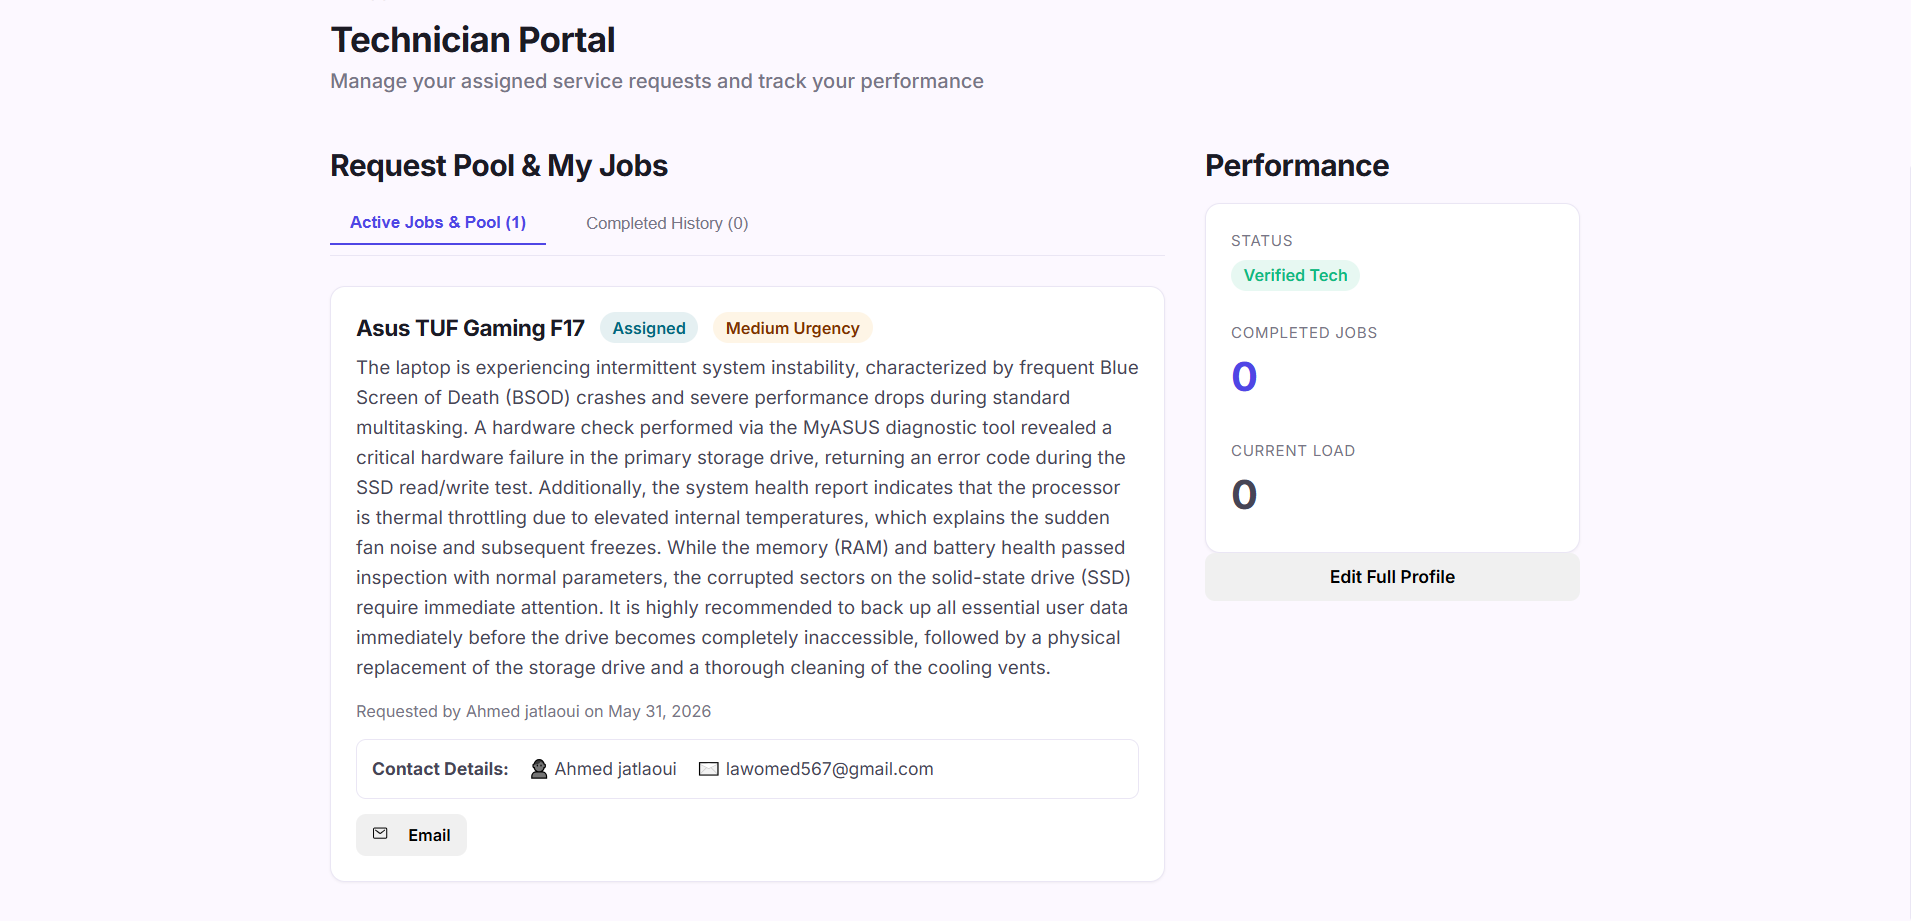
\includegraphics[width=0.48\textwidth]{images/technician Portal.PNG}
 \caption{Web interfaces -- Technician approval dashboard and technician portal request pool}
 \label{fig:web_matching}
 \end{figure}

\subsection{Mobile Interfaces}

The mobile interface shown in Figure~\ref{fig:mobile_matching} highlights the workspace where technicians browse pending tickets, claim jobs, and report progress.

\begin{figure}[!htbp]
\centering
\includegraphics[width=0.5\textwidth]{images/mobile_matching.png}
\caption{Mobile interface -- Maintenance requests and technician job dashboard}
\label{fig:mobile_matching}
\end{figure}

\section{Conclusion}

In Release 5, we completed the ticketing and technician coordination modules. This bridges digital self-service troubleshooting with physical repair logistics. With the final release implemented, the next chapter details our project conclusions and future milestones.


\chapter*{General Conclusion and Perspectives}
\addcontentsline{toc}{chapter}{General Conclusion and Perspectives}

Our team developed PRO-WISE to streamline appliance technical support and coordinate on-site repairs. We structured the project as a monorepo that connects manufacturers, field technicians, and customers into one cohesive, context-aware environment.

To build the platform modularly and systematically, we split the implementation into five successive sprints:
\begin{itemize}
    \item \textbf{Core Security}: We implemented role-based access control and stateless token authentication to secure backend API routes from the start.
    \item \textbf{Content Management}: We designed category catalogs, markdown manuals, and interactive guide editors for brand administrators.
    \item \textbf{Engagement and Logs}: We built feedback review forms, real-time WebSocket notifications, and background database audit logs.
    \item \textbf{Intelligent Layer}: We integrated the Google Gemini API~\cite{gemini} for vector semantic search, automated compatibility matching, and real-time community content moderation.
    \item \textbf{Field Support}: We created a full-lifecycle support ticketing flow and dedicated mobile jobs dashboards for repair technicians.
\end{itemize}

Running a Sails.js backend separately from the React web dashboard and React Native mobile app allows us to host and scale services independently. Comparing PRO-WISE with existing systems like iFixit and GE Appliances highlights how linking direct QR code scans to vector semantic search models modernizes technical maintenance.

\section*{Perspectives and Future Work}

We mapped out several technical and functional updates to expand the platform in the future:

\subsection*{Technical Enhancements}
\begin{itemize}
    \item \textbf{Fine-Tuned Embeddings}: We plan to train local transformer models on domain-specific engineering jargon to make search queries even more precise.
    \item \textbf{In-App Chat}: We want to add WebSocket chat rooms where clients and technicians can coordinate repairs in real-time.
    \item \textbf{Smart Dispatching}: We will use geolocation queries to suggest nearby technicians, optimizing response times.
    \item \textbf{Offline Manuals}: We plan to sync local databases on the mobile app so technicians can access guides even in remote areas without connection.
\end{itemize}

\subsection*{Functional Extensions}
\begin{itemize}
    \item \textbf{Integrated Payments}: We want to connect payment gateway APIs to handle diagnostic fees and repair billing directly.
    \item \textbf{Domain Expansion}: We plan to adapt the database metadata schemas to support other fields like IT helpdesks and heavy machinery maintenance.
\end{itemize}

\subsection*{Final Remarks}

The PRO-WISE architecture proves that pairing AI semantic models with strict database and role constraints works exceptionally well for real-world support systems. This platform lays a solid foundation for next-generation hardware diagnostics and field service automation.

\renewcommand{\bibname}{Webography}
\begin{thebibliography}{99}
\raggedright
\addcontentsline{toc}{chapter}{Webography}

\bibitem{nodejs}
Node.js Foundation. (2026). \textit{Node.js v20 LTS Runtime Environment Documentation}. Available online at: \url{https://nodejs.org/en/docs} [Accessed May 2026].

\bibitem{sailsjs}
Sails.js Core Team. (2026). \textit{Sails.js Framework Reference Manual for Enterprise Node.js Applications}. Available online at: \url{https://sailsjs.com/documentation} [Accessed May 2026].

\bibitem{mongodb}
MongoDB, Inc. (2026). \textit{MongoDB Manual and Developer Reference Guide}. Available online at: \url{https://www.mongodb.com/docs} [Accessed May 2026].

\bibitem{react}
Meta Open Source. (2026). \textit{React Library Developer Reference and UI Component Design Guides}. Available online at: \url{https://react.dev} [Accessed May 2026].

\bibitem{vite}
Vite Core Team. (2026). \textit{Vite Frontend Build Tooling Guide}. Available online at: \url{https://vite.dev/guide} [Accessed May 2026].

\bibitem{typescript}
Microsoft Corporation. (2026). \textit{TypeScript Language Specification and Reference Documentation}. Available online at: \url{https://www.typescriptlang.org/docs} [Accessed May 2026].

\bibitem{redux}
Redux Core Team. (2026). \textit{Redux Toolkit Standard Developer Guides}. Available online at: \url{https://redux-toolkit.js.org} [Accessed May 2026].

\bibitem{expo}
Expo Project. (2026). \textit{Expo Framework Development Documentation for React Native Application Suites}. Available online at: \url{https://docs.expo.dev} [Accessed May 2026].

\bibitem{reactnative}
Meta Open Source. (2026). \textit{React Native Framework Documentation}. Available online at: \url{https://reactnative.dev/docs/getting-started} [Accessed May 2026].

\bibitem{jwt}
Auth0, Inc. (2026). \textit{JSON Web Tokens (JWT) Architecture and Specifications Overview}. Available online at: \url{https://jwt.io/introduction} [Accessed May 2026].

\bibitem{gemini}
Google LLC. (2026). \textit{Google Gemini API Reference Guide and Vector Embeddings Documentation}. Available online at: \url{https://ai.google.dev/gemini-api/docs} [Accessed May 2026].

\bibitem{qrcode}
Denso Wave Incorporated. (2026). \textit{QR Code Standard Technology and Features Overview}. Available online at: \url{https://www.qrcode.com/en/about} [Accessed May 2026].

\bibitem{ifixit}
iFixit Community. (2026). \textit{iFixit Open Source Hardware Repair Manuals and Guides}. Available online at: \url{https://www.ifixit.com/Guide} [Accessed May 2026].

\bibitem{geappliances}
General Electric Company. (2026). \textit{GE Appliances Technical Support and Appliance Field Maintenance Services}. Available online at: \url{https://www.geappliances.com/ge/service-and-support} [Accessed May 2026].

\bibitem{mongodb_multitenant}
MongoDB, Inc. (2026). \textit{Multi-Tenant SaaS Database Design Patterns in MongoDB}. Available online at: \url{https://www.mongodb.com/blog/post/building-multitenant-saas-applications-mongodb} [Accessed May 2026].

\bibitem{scrumguide}
Schwaber, K., \& Sutherland, J. (2020). \textit{The Scrum Guide: The Definitive Guide to Scrum: The Rules of the Game}. Available online at: \url{https://scrumguides.org} [Accessed May 2026].

\bibitem{umlguide}
Booch, G., Rumbaugh, J., \& Jacobson, I. (2005). \textit{The Unified Modeling Language User Guide (2nd Edition)}. Addison-Wesley Professional.

\bibitem{bcrypt}
Provos, N., \& Mazières, D. (1999). \textit{A Future-Adaptable Password Scheme}. In Proceedings of the 8th USENIX Security Symposium.

\bibitem{oauth2}
Hardt, D. (2012). \textit{The OAuth 2.0 Authorization Framework}. IETF RFC 6749. Available online at: \url{https://datatracker.ietf.org/doc/html/rfc6749} [Accessed May 2026].

\bibitem{tls13}
Rescorla, E. (2018). \textit{The Transport Layer Security (TLS) Protocol Version 1.3}. IETF RFC 8446. Available online at: \url{https://datatracker.ietf.org/doc/html/rfc8446} [Accessed May 2026].

\bibitem{rag}
Lewis, P., Perez, E., Piktus, A., Petroni, F., Lewis, M., Riedel, S., \& Kiela, D. (2020). \textit{Retrieval-Augmented Generation for Knowledge-Intensive NLP Tasks}. In Advances in Neural Information Processing Systems, 33, 9459-9474.

\bibitem{manning2008}
Manning, C. D., Raghavan, P., \& Schütze, H. (2008). \textit{Introduction to Information Retrieval}. Cambridge University Press.

\bibitem{bge_embeddings}
Xiao, S., Liu, Z., Zhang, G., \& Sun, J. (2023). \textit{C-Pack: Packaged Resources for Chinese Natural Language Processing}. arXiv preprint arXiv:2309.07597.

\bibitem{llama3}
Meta AI. (2024). \textit{Introducing Llama 3: The Next Generation of Meta's Open Source Large Language Model}. Available online at: \url{https://llama.meta.com} [Accessed May 2026].

\bibitem{aws_ec2}
Amazon Web Services. (2026). \textit{Amazon Elastic Compute Cloud (EC2) Documentation}. Available online at: \url{https://aws.amazon.com/ec2} [Accessed May 2026].

\bibitem{git}
Chacon, S., \& Straub, B. (2014). \textit{Pro Git (2nd Edition)}. Apress. Available online at: \url{https://git-scm.com/book/en/v2} [Accessed May 2026].

\bibitem{vscode}
Microsoft Corporation. (2026). \textit{Visual Studio Code Developer Documentation}. Available online at: \url{https://code.visualstudio.com/docs} [Accessed May 2026].

\bibitem{overleaf}
Overleaf Project. (2026). \textit{Overleaf LaTeX Authoring Platform Guide}. Available online at: \url{https://www.overleaf.com/learn} [Accessed May 2026].

\bibitem{drawio}
JGraph Ltd. (2026). \textit{Draw.io / diagrams.net Diagramming Software Reference}. Available online at: \url{https://www.drawio.com/doc} [Accessed May 2026].

\bibitem{nginx}
Nginx, Inc. (2026). \textit{NGINX Core Web Server and Reverse Proxy Reference}. Available online at: \url{https://nginx.org/en/docs} [Accessed May 2026].

\bibitem{lighthouse}
Google LLC. (2026). \textit{Google Lighthouse Auditing Tool Documentation}. Available online at: \url{https://developer.chrome.com/docs/lighthouse/overview} [Accessed May 2026].

\bibitem{eslint}
ESLint Foundation. (2026). \textit{ESLint Linter for JavaScript and TypeScript Reference Guide}. Available online at: \url{https://eslint.org/docs} [Accessed May 2026].

\end{thebibliography}

\end{document}
